\documentclass[a4paper,12pt, english,twoside]{book}% norsk istedefor english
%\usepackage{ucs}
\usepackage[utf8]{inputenc}%utf8x
\usepackage{fontenc}%[T1]
\usepackage{babel,graphicx,subfigure,epsfig}%,uioforside},babel hvis norsk
\usepackage{amssymb,psfrag,amsmath,wick}
\usepackage{wrapfig,algorithm,algorithmic}
\usepackage{verbatim}
%\usepackage{a4wide}
\usepackage{bezier}
\usepackage{color}  
\usepackage[pdftex,colorlinks=true,bookmarks=true,linkcolor=blue]{hyperref}

\newcommand{\be}{ \begin{equation}}
\newcommand{\ee}{ \end{equation}}
\newcommand{\mc}{ \mathcal }
\newcommand{\bra}[1]{\langle #1|}
\newcommand{\ket}[1]{|#1\rangle}
\newcommand{\braket}[2]{\langle #1|#2\rangle}
\newcommand{\beq}{\begin{equation*}}
\newcommand{\eeq}{\end{equation*}}
\newcommand{\ds}{\displaystyle{\not}}
\newcommand{\bsp}{\begin{split}}
\newcommand{\eesp}{\end{split}}
\newcommand{\matr}[1]{{\bf \cal{#1}}}
\newcommand{\OP}[1]{{\bf\widehat{#1}}}
\newcommand{\sd}{$}

%\title{AB INITIO STUDIES OF INFINITE MATTER}
%\author{Johannes Rekkedal}
%\date{}


 \renewcommand{\rmdefault}{ptm} % Times
 \newcommand{\clearemptydoublepage}{\newpage{\pagestyle{empty}\cleardoublepage}}
 \newcommand{\mymarkright}[1]{\markright{\thesection\ -- #1}}
 \newcommand{\mymarkboth}[2]{\markboth{#1}{#2}}
 %
 % redefine page style
 %
 \usepackage{fancyhdr}
 % choose pagestyle fancy and define it
 \pagestyle{fancy}
 \fancyhead{} %clear everything
 \fancyfoot{} %clear everything
 \addtolength{\headheight}{1.5pt}
 \addtolength{\headwidth}{2.5\marginparsep}
 \renewcommand{\chaptermark}[1]{\mymarkboth{#1}{}}
 \renewcommand{\sectionmark}[1]{\mymarkright{#1}}
 \fancyfoot[EL,OR]{\bfseries\itshape\thepage}
 \fancyhead[EL]{\nouppercase{\bfseries\itshape\leftmark}}
 \fancyhead[OR]{\nouppercase{\bfseries\itshape\rightmark}}
 \renewcommand{\headrulewidth}{1pt}
 % redefine plain page style. used on first pages of chapters et.c.
 \fancypagestyle{plain}{\fancyhf{}\fancyfoot[EL,OR]{\bfseries\itshape\thepage}%
 \renewcommand{\headrulewidth}{0pt}
 }
 %
 % redefine bullet. looks better with an ndash.
 %
 \renewcommand{\labelitemi}{\bfseries--}
 %
 % define styles for section and subsection headings
 %
 %\font\tenhv  = phvb at 12pt
 %\newcommand{\hvfont}{\fontfamily{phv}\selectfont}
 %\newcommand{\hvfont}{\fontfamily{phv}\fontseries{bc}\selectfont}
 \newcommand{\secstyle}{\normalfont\itshape\bfseries\large}
 %\newcommand{\secstyle}{\hvfont\itshape\large}
 \newcommand{\subsecstyle}{\normalfont\itshape\large}
 \newcommand{\paragraphstyle}{\normalfont\itshape}
 %
 % redefine look of sections, subsections and paragraphs.
 %

\makeatletter
 \renewcommand{\section}{%
 \@startsection
   {section}%   the name
   {1}%         the level
   {0pt} %{-\Myindent}%       the indent
   {-2\baselineskip}%   beforeskip
   {\baselineskip}%    afterskip
   {\secstyle}}%   style
 \renewcommand{\subsection}{%
 \@startsection
   {subsection}%   the name
   {2}%         the level
   {0pt}%{-\Myindent}%       the indent
   {-\baselineskip}%   beforeskip
   {0.5\baselineskip}%    afterskip
   {\subsecstyle}}%   style
 \renewcommand{\paragraph}{%
 \@startsection
   {paragraph}%   the name
   {4}%         the level
   {0pt}%{-\Myindent}%       the indent
   {-\baselineskip}%   beforeskip
   {-1em}%    afterskip
   {\paragraphstyle}}%   style
 \makeatother
 %%
 %% modify margins...
 %%
 \addtolength{\oddsidemargin}{-0.5cm}
 \addtolength{\evensidemargin}{-1.0cm}
 \addtolength{\textwidth}{0.5cm}


\begin{document}
%\maketitle
\thispagestyle{empty}
\begin{center} \vspace{1cm}
    \textbf{\Large{\mtitle}}\\ \vspace{0.5cm}
    \small{by}\\ \vspace{0.5cm}
    \large{\mauthor}\\ \vspace{4.4cm}
    \large{THESIS}\\ \vspace{0.3cm}
    \small{for the degree of}\\ \vspace{0.3cm}
    \large{MASTER OF SCIENCE}\\ \vspace{0.7cm}
    
\includegraphics[scale=1.0]{../Images/UiO_Segl_pms485.eps} \\ \vspace{0.5cm}
    \large{Faculty of Mathematics and Natural Sciences \\ University of Oslo} \\ \vspace{0.5cm}
    \small{\mdate}\\ \vfill
\end{center}
\newpage
\vspace*{\fill}
{\setlength{\parindent}{0cm}
All illustrations in this thesis are created using the TikZ package \cite{tantau_graph_2013} if nothing else is specified. The plots are produced using a controversial combination of Matplotlib \cite{hunter_matplotlib:_2007} and PGFPlots \cite{tantau_graph_2013}.\bigskip

Effort was made to follow the ISO 80000-2:2009 standard for mathematical signs and symbols \cite{iso/tc_12_iso_nodate}, and the ISO 80000-9:2009 standard for quantities and units in physical chemistry \cite{iso/tc_12_iso_nodate-1}.\bigskip

The \LaTeX\, document preparation system was applied for typesetting.
} 
\newpage
\section*{Abstract}
Being able to solve the many-body Schrödinger equation accurately, in principle all physics and chemistry could be derived from first principles. However, exact wave functions of realistic and interesting systems are in general unavailable because they are non-deterministic polynomial-hard to compute \cite{troyer_computational_2005}, implying that we need to rely on approximations. The variational Monte Carlo (VMC) method is widely used for ground state studies, but requires a trial wave function ansatz which must trade off between efficiency and accuracy. The method has also many common features with machine learning algorithms, and as neural networks have shown impressive power as function approximators, the idea is to use a neural network as the trial wave function guess. For fermionic systems, like electronic structure systems, the wave function needs to obey Fermi-Dirac statistics, which typically is achieved using a Slater determinant. As a neural network hardly can model this feature, our approach is to replace the single-particle functions in the Slater determinant with restricted Boltzmann machines (RBM). To model the cusp correctly, correlation factors in the forms of a simple Jastrow factor and the well-known Padé-Jastrow factor were added, abbreviated RBM+SJ and RBM+PJ, respectively.

Our primary focus is on closed-shell circular quantum dots, where we compute the ground-state energy and electron density for two-dimensional systems with up to $N=90$ electrons and three-dimensional systems with up to $N=70$ electrons. The energy obtained by the RBM was reasonably close to experimental results, and it gradually got closer as we added more complex correlation factors. For the RBM+PJ, the energy was found to be lower than the VMC-energy for small dots, but for larger dots it was slightly higher. However, the one-body density profile reveals that the RBM gives more distinctly located electrons compared to the VMC method, which can be explained by the way the RBM models the correlations. From the two-body density profile, we also observe that the repulsive interactions get more significant as we add a Jastrow factor. Based on the electron densities and the energy distribution between kinetic and potential energy, it is certain that the various methods provide different electron configurations. For low-frequency dots, the electron density undergoes a phase transformation with an additional radial peak compared to high-frequency dots, indicating "incipient" Wigner localization.

The computational time consumption was found to be favorable for the RBM for small systems and VMC for large systems, which can be explained by the exploding number of variational parameters in the RBM as the system sizes increase. RBMs with Jastrow factors were significantly more computationally expensive than the other methods, and apparently, there is no point in adding a simple Jastrow factor when we can add a more complicated Jastrow factor.

\thispagestyle{empty}
\cleardoublepage

\section*{Acknowledgements}
After five exciting years at Blindern my time here has come to an end, and on that occasion I would like to acknowledge some people who have been influential throughout the studies. First, I would like to thank my excellent supervisor, Morten Hjorth-Jensen, whom I luckily got to know three years ago. From day one, you took me under your wing and enthralled me with your eager, massive knowledge and work ethic. Few things make me more motivated than talking with you, be it in real-life at Blindern or through video conversations from whatever place you happen to be at.

I would also like to acknowledge the support I have got from my parents and my sister. Albeit the schedule has been filled up and I have not spent as much time with you as I wanted, you have always been supportive and stand up for me anytime I need some help. Thanks to my friends (you know who you are) who are always ready for a beer (or ten) whenever I seek to disconnect from the studies. Those moments filled with lively discussions and dark humor have kept me motivated throughout the studies, which has been absolutely crucial.

The computational physics group is a funny composition of different people with a shared predilection for physics and programming. There are so many talented guys in the group, and I have really appreciated spending early mornings and late nights with you. Last, but not least, I would also like to thank my high school teacher, Jens Otto Opaker, who with his enthusiasm and dedication, got me hooked on science in the first place.

\iffalse
\textcolor{red}{I have always believed that everything has a reason, which I used to point out whenever people talked about things that could not easily be explained. First when I was introduced to quantum mechanics, I realized that it might not be that simple, which is one of the reasons why this beautiful theory caught my attention. Even though my philosophy has changed to a less deterministic direction, I still like to think that everything can be explained out of some first principles.}
\fi
    
\thispagestyle{empty}
\cleardoublepage

\newpage

{%
    %\microtypesetup{protrusion=false}
    \tableofcontents
    %\microtypesetup{protrusion=true}
    \thispagestyle{empty}
    \clearpage}%

\thispagestyle{empty}
\clearpage



\clearemptydoublepage
%\fysikkforside{}
%\uioforside[inst = Department of Physics]
% maa kompilere med latex istedefor pdflatex for at uioforside 
%skal virke
%\pagenumbering{roman}
\chapter*{Acknowledgements}
First of all I have to thank my wife Nubia and my family for being so patient with me in this stressful time.\\
\\
I would like to thank my supervisor Morten Hjorth-Jensen. I am very grateful 
for all the help and guidance he has given me during my two years as a master 
student. \\
\\
I am very grateful for my fellow students. I would like to thank the people who
share the office with me, Rune, Lene, Patrick and Islen. I would especially thank Gustav Jansen for reviewing the chapter on coupled cluster theory and for 
some interesting discussions at Oak Ridge.\\
\\
Finally I have to thank Jan Lindroos for reviewing the thesis and for all the
interesting discussion we have had about everything regarding physics and 
mathematics.



\clearemptydoublepage
\chapter*{Notation}

\section*{Units}
We will in all chapters except the second, regarding quantum mechanics, work with units, where
\beq
\hbar=c=1
\eeq
In this system,
\begin{align}
		&\mbox{[length]}=\mbox{[time]}=\mbox{[energy]}^{-1}=\mbox{[mass]}^{-1}.\notag
\end{align}
The mass $m$ of a particle is therefore equal to its rest energy ($mc^2$).

\section*{Vectors}
Vectors are boldfaced, $\bold v$ is an ordinary vector in three dimensions. Four vectors are denoted by a Greek letter, $A^\mu$, where $\mu=(0,1,2,3)$
\beq
A^\mu=\left(A^0,\bold A\right)~\mbox{and}~ A_\mu=(-A^0,\bold A)
\eeq


\section*{Summation convention}
We use Einstein summation conventions, where equal upper and lower indices are summed over, Greek letters are summed from zero to three,
\beq
A^\mu B_\mu=\sum_{\mu=0}^3A^\mu B_\mu.
\eeq

\section*{Spin and isospin}
The Pauli spin matrices $\mathbf\sigma$ are defined as
\beq
\sigma^i=\begin{pmatrix} 0 & 1\\1 & 0\end{pmatrix},~
		\sigma^j=\begin{pmatrix} 0 & -i\\i & 0\end{pmatrix}~\mbox{and}~
				\sigma^k=\begin{pmatrix} 1&0\\0&-1\end{pmatrix}.		
\eeq
The isospin matrices $\mathbf\tau$ are defined as 
\beq
\tau^i=\begin{pmatrix} 0 & 1\\1 & 0\end{pmatrix},~
		\tau^j=\begin{pmatrix} 0 & -i\\i & 0\end{pmatrix}~\mbox{and}~
				\tau^k=\begin{pmatrix} 1&0\\0&-1\end{pmatrix}.		
\eeq
\section*{Commutators}
A commutator between two operators $A$ and $B$  is defined as
\beq
[A,B]=AB-BA.
\eeq
The anticommutator is defined as
\beq
\{A,B\}=AB+BA.
\eeq

\clearemptydoublepage
\tableofcontents
\clearemptydoublepage
%\listoffigures
%\listoftables


%\pagenumbering{arabic}
\chapter{Introduction}
\label{introduction}

\section{Historical Background}

In order to make useful progress the equations must be solved numerically. 
About 2400 years ago, the Greek philosopher Anaxagoras invented the
idea that matter could be devided into infinitly small parts;
\emph{spermata}. 
This concept was expanded a few years later by
Democritus, who believed matter was composed of tiny particles of
finite size or mass. He called the invisible particles of matter
\emph{atoms}; which in greek means 'undevidable'. 
No experimental techniques needed to test the atomic
hypotheses existed at the time, and there was no advance in the
understanding of atoms for more than 2000 years! 

\subsection*{Discovery of the Atom}

In 1807, John Dalton postulated that atoms of each element had a
unique mass. Dalton's atomic theory contained a simple prediction for
the case where two elements combine to form two different compounds;
\emph{The Law of Multiple Proportions}. (For example, 16 g of oxygen, O,
combines with 12 g of carbon, C, to form carbonmonoxide, CO, and
32 g of O combines with 12 g of C to form carbondioxide, CO$_2$).
%
\newline
%
A great leap in the understanding of the structure of matter was made
in 1811 by Amedeo Avogadro. Avogadro correctly hypothesized that the
particles of a gas were small compared to the distance between the
particles. He determined that these particles were often made up of
more than one atom; \emph{molecules}. This important result is the
basis for the \emph{Ideal Gas Law}, and the discovery provided a
systematic method for measurement of the atomic mass numbers.

\subsection*{The Periodic Table}

In 1869, Dmitri Mendeleev made the first classification of the
elements. The elements were ordered with increasing atomic mass
number, and placed in several columns according to their chemical
properties. Mendeleev discovered some gaps, that made him to correctly
predict the existance of undiscovered elements!

\subsection*{Discovery of the Electron}

A type of radiation, called \emph{cathode rays}, was observed to be
emitted from metallic surfaces when voltage was applied. At the end of
the 19$^{th}$ century there was much speculation about the fundamental
properties of the cathode rays. One school of thought held the belief
that cathode rays were particles, while the other school believed it
was a wave-phenomenon. In 1897, Joseph John Thomson preformed a
definitive set of experiments that proved that cathode rays had
a particle behavior. Thomson developed the necessary technique to
observe the deflection of chatode rays in an electric field. This led
to the interpretation of chatode rays as charged particles;
\emph{electrons}.

\subsection*{Measurement of the Electric Charge}

In 1909, Robert Millikan made the first accurate measurement of the
electron charge. \emph{The Millikan Oil-Droplet Experiment} was
performed by spraying tiny droplets of oil between two conducting
plates. By switching the electric field between the two plates on and
off, Millikan was able to accuratly estimate the electron charge. The
result of numerous measurements by Millikan, was that the charge was
allways an integer multiple of $1.6 \cdot 10^{-19}C$.
Figure \ref{oil_droplet} illustrates the forces acting on the
oil-droplet.

\begin{figure}[hbtp]
\begin{center}
  \epsfig{file=Introduction/oil_droplet.eps, height=5cm}
  \caption{
    Forces on an oil-droplet in: \newline
    \hspace*{1.5cm}
           a) Free fall          \newline
    \hspace*{1.5cm}
	   b) Electric field     \newline
    (G=Gravitation, D=Drag, E=Electric force)
  }
  \label{oil_droplet}
\end{center}
\end{figure}

His results were systematically low by about 4\% due to inaccurate
knowledge of the coefficient of viscosity. \newline
The electron charge is -e,
where $e = 1.602 \cdot 10^{-19}C$. All free particles are observed to
have values of electric charge equal to an integer times the
fundamental charge e:

\begin{equation*}
  q=n e
\end{equation*}

where the integer $n=\dots,-1,0,1,\dots$ is the electric charge
\emph{quantum number}.

\subsection*{The Nucleus}

In 1912, Ernest Rutherford and his associates discovered that the
positive charge of the atom is concentrated in a \emph{nucleus}. The
charge of the $\alpha$ particle, discovered by Becquerel, was
determined to be $2e$, and the mass of the $\alpha$ particle was
determined to be about four times the mass of the hydrogen
atom. \newline
A new particle with zero electric charge was discovered by bombarding
beryllium atoms with $\alpha$ particles. James Chadwick showed that
the new particle, the \emph{neutron}, had mass nearly equal to that of
the \emph{proton}.

\subsection*{The Bohr Model of the Atom}

In 1913, Niels Bohr made the first qunatitatively successful model of
the atom. Inspired by the work of Rutherford, Bohr made a planetary
model of the atom; with electrons moving in circular orbits about the
nucleus. This model may seem quite simple in retrospect, but for the
time it was a great advancement of science. In addition to the
classical circular orbits, the second part of Bohr's atomic model
contains a bold hypothesis of new physics. The new physics recognizes
that \emph{angular momentum} is \emph{quantized}; it can take only
certain values:

\begin{equation*}
  L = mvr = n \hbar
\end{equation*}

where $n$ is a positive integer. Solving the energy equations result
in orbits of radius:

\begin{equation*}
  r_n = \frac{n^2\hbar^2}{mke^2}
\end{equation*}

where the \emph{Bohr radius}

\begin{equation*}
  a_0 \equiv r_1 = \frac{\hbar^2}{mke^2} \approx 0.053 nm
\end{equation*}

is in the correct order of magnitude for the size of the atom!

{\bf Planc }





%               The Two First Excited states of Helium
\subsection{The Two First Excited states of Helium}

We will not make any calculations regarding exited states in this
thesis, but it is a really important issue in quantum mechanics. The
ground state energy does not tell much about the 
chemical properties of the atom on its own. Therefore good
approximations of the exited states are needed. Also, when discussing
different numerical approaches for solving the many body-problem,
including linear combinations of exited states may greatly improve
some original approximation to the ground state. Furthermore,
understanding how we include exited states is important for fully
understanding the application of the Slater determinant.
\newline
%
\newline
The state of helium with the $1s$ and the $2s$ orbitals occupied
with one electron each. 








The construction of the
periodic table in the second half of the $19^{\mathrm{th}}$ century
was based on the chemical properties of the different atoms. These
properties were not understood until the development of quantum
mechanics. The electrons are filled from the energetically lowest
orbitals. In the $s$ orbitals only two electrons of different
spins are allowed. Disregarding electron repulsion this would imply
that twice the energy is needed in removing an electron from ground
state helium than from the ground state hydrogen. This due to the 
double electric charge of the helium nucleus. The ionization energy of
hydrogen is $13.60 eV$ and the ionization energy of helium is $24.58
eV$ (ref. \cite{atkins2003}). The electron repulsion thus reduce the
ionization energy by almost $10\%$.
\newline
%
\newline
The early development of quantum theory may be summarized through the
four postulates of quantum mechanics.


%*************** The Postulates of Quantum Mechanics **************
%*
%*
\section{The Postulates of Quantum Mechanics}

A common formulation of quantum mechanics is by means of linear
algebra. In this formulation every state is represented as a (usually
infinite dimensional) complex vector, and an operator is represented
as a complex, linear and hermitian matrix. 
The postulates of quantum mechanics fall naturally into two sets: the
first three, which tell us how the system is depicted at a given time,
and the fourth, which specifies how this picture changes with time. 
\newline

%*                     The First Postulate                              *
%\subsection{The First Postulate}

{\bf \large Postulate 1}
\emph{
The state of a quantum mechanical particle is described by a vector
$\Psi$ in a Hilbert space ${\cal H}$. All the possible states of the
particle are ${\cal H}$ except the zero vector.
\newline
}

The first postulate states that a particle is described as a vector in
the Hilbert space. So a particle with finite degrees of
freedom $\mathbf{x}$ and $\mathbf{p}$ in classical
mechanics, now has infinite degrees of freedom. 
\newline

%*                     The Second Postulate                              *
%\subsection{The Second Postulate}

{\bf \large Postulate 2}
\emph{
Every observable are represented by an Hermitian linear operator in
${\cal H}$. For every classical dynamical variable
$\omega(\mathbf{x},\mathbf{p})$ there is a corresponding quantum
mechanical operator $\Omega$  obtained by operator substitution of the
fundamental position and momentum operators $\mathbf{X}$ and
$\mathbf{P}$, respectively: 
}
%
\begin{equation*}
  \Omega(\mathbf{X},\mathbf{P}) = \omega(\mathbf{x} \to
  \mathbf{X},\mathbf{p} \to \mathbf{P})
\end{equation*}
%
\emph{
The components of $\mathbf{X}$ and $\mathbf{P}$ are operators defined
through the fundamental commutation relation
}

\begin{equation*}
  \left[ X_i, P_j \right] = i \hbar \delta_{ij}
\end{equation*}

The second postulate tell us how to to move from the classical to the
quantum mechanical picture. The observables (or measurable quantities)
are defined through an operator. This operator may be obtained by
simple substitution of the position and the momentum of the
corresponding classical observable.
\newline

%*                     The Third Postulate                              *
%\subsection{The Third Postulate}

{\bf \large Postulate 3}
\emph{
The only possible values obtainable in an (ideal) measurement of an
observable $\Omega$ are its eigenvalues $\omega_n$. Each have a
probability
}
%
\begin{equation*}
  P(\omega_n) = \frac{\int \Psi^* \Phi_n }{\int \Psi^* \Psi }
\end{equation*}
%
\emph{
with $\Phi_n$ the eigenfunction corresponding to the eigenvalue
$\omega_n$. Immediately after a measurement the state collapses into
$\Phi_n$.
}
\newline

The third postulate tells what may be extracted from the quantum
mechanical picture by means of measurements. Note that the eigenvalues
may either have a continuous spectrum or be \emph{quantized}.
\newline


%*                     The Fourth Postulate                              *
%\subsection{The Fourth Postulate}

{\bf \large Postulate 4}
\emph{
The time development of the quantum state $\Psi$ is given by the time
dependent Schr\"odinger equation,
}

\begin{equation*}
  \hat{H} \Psi(\mathbf{x},t) = i\hbar \frac{\delta}{\delta
  t}\Psi(\mathbf{x},t) 
\end{equation*}

The fourth and final postulate defines the Schr\"odinger
equation. This equation describes how the quantum mechanical state
evolve in time.
\newline




 % introduction.tex
\clearemptydoublepage
%\part{Theoretical Foundations}
\chapter{Some historical aspects regarding quantum mechanics}

It is not easy to give a short presentation of quantum mechanics, it is a rather huge and strange subject. When speaking about quantum mechanics we should always keep in mind what Feynman said, "I think it is safe to say that no one understands Quantum Mechanics". 
The world quantum mechanics treats, is a small world, the world of very small objects, such as electrons, atoms and nuclei. \\
\\
The most natural point to start when reviewing quantum mechanics is maybe how
it started. It started with light, the feature of light has long been an
important part in physics. The explanation of light has long been alternating
between the definition of light as a wave picture and a corpuscular picture.  
Light has
interested man in maybe all of time. The Iraqi born scientist Ibn
al-Haytham (965-1040), which in the west goes under the name Alhazen, in his
Book of optics, treats light as energy particles that travel in straight
lines at a high but finite speed \cite{alhazen}. Issac Newton followed the
particle interpretation of light, however he understood that he had to
associate light with waves in order to explain the diffraction properties of
light.
Robert Hooke and Christian Huygens believed light to be waves and worked out their own and separate theories of light. \\
\\
In our everyday life we can see a clear distinction between waves and
particles, waves exhibit a phenomena called interference which particles do
not. Interference occurs when two waves traveling in the same medium meet. As
an example we can look at two sine waves traveling in opposite directions and
with the same amplitude. If these two waves meet when both are on their
maxima the net result of the waves will be a peak with twice the amplitude of
the waves, which is an example of constructive interference. If the waves are
completely out of phase when they meet, one of the waves is phasing upwards
and the other downwards, the net result will be a zero peak, this type of
interference is called destructive. There will  be constructive interference
when the displacement of the two waves are in the same direction and
destructive when the displacement of the waves are in opposite directions.\\ 
\\
There are two experiments which are rather crucial in quantum mechanics, and
revolutionized physics.  The photoelectric effect, explained by Einstein,
for which he got the Nobel prize and the double-slit experiment.  In the
photoelectric effect light is scattered on metal and collides with the
electrons. The collisions can be registered by measuring the current. If light
were to be a wave the average energy measured of a single electron should
increase with the intensity, the phenomena observed was a surprise. The energy
of the ejected electrons did not at all depend on the intensity. It was found
that it depends on the frequency of the light waves, and that below a
certain frequency there were no ejected electrons. Einstein resolved this
paradox by proposing that light consists of individual quanta, which now are
called photons. These photons carry energies which come in discrete quanta. The
energy can just come in amounts of \sd \hbar \omega\sd, where \sd \hbar\,\sd
goes under the name of Planck's constant, and \sd\omega\,\sd is the frequency
of the light. By varying the frequency of light it was also discovered that
the momentum $p$ is proportional to the wavenumber $k$ and a multiple of planck's constant, $p=\hbar k$. With these expressions of energy and momentum it was
deduced from Einstein's famous equation for energy \sd E=\sqrt{p^2c^2
+m^2c^4}\sd\, that the photon is massless. \\
The double slit experiment with light shows the opposite behavior. 
In the double slit experiment light waves are send in a way such that
they are incident normally on a screen with two slits \sd S_1\,\sd and \sd
S_2\sd, which are a distance \sd a\,\sd apart. If only slit \sd S_1\,\sd is
open an intensity pattern \sd I_1\sd, is observed. And likewise if only \sd
S_2\,\sd is open an intensity pattern \sd I_2\,\sd is observed. When both of
the slits are left open an interference pattern is observed, what is crucial is
that the intensity \sd I_{1+2}\,\sd is not \sd I_1 +I_2\sd \,  which would be
the case if light were to be particles.\\
\\
This seemingly contradictory properties of light was then interpreted as the
particle wave duality of light. The Copenhagen interpretation, which states
that particles such as photons, but also electrons and other small particles
have both wave and particle properties. The particles obey a complementary principle
which states that an experiment can show particle like properties and another
wave like properties, but none can show them both at the same time.  This is
the most accepted interpretation of quantum mechanics, however Einstein has
always questioned this interpretation and together with Podolsky and Rosen
proposed a paradox later called the EPR paradox. We will not go through this
paradox, it can be read in any book treating quantum theory. When Aspect did
experiments on Bell's inequalities, he showed the consistency of the Copenhagen interpretation. However Afshar claims that he
in a recent experiment has showed both particle and wave properties at the same time,
Refs. \cite{afshar-2005-5866,afshar-2006-810}.\\ 
\\
Now the time has come to say something about the postulates and mathematics of
quantum mechanics.  The first postulate is that the state of a particle is
represented by a vector, or ket \sd\ket{\Psi(t)}\sd\, in the Hilbert space, \sd
\mathcal H\sd. All properties of the particle are contained in this wave
function. Properties of the particles which can be measured, such as position,
energy and velocity are in quantum mechanics called observables and are
represented by operators.  If a particle is in a state \sd \ket{\Psi}\sd, the
measurement of a variable \sd O\sd, will yield us one of the eigenvalues
\sd o\sd. The probability that the eigenvalue \sd o\sd \, is measured is
\sd|\braket{o}{\Psi}|^2\sd. After the measurement, the state of the system
changes from the state \sd \ket{\Psi}\sd\, to the state \sd\ket{o}\sd. This
effect is called the collapse of the state.  Complications caused by the
collapse of the wave function arise when measuring different observables. If we
measure an observable \sd \lambda\sd, just after the observable \sd \omega\sd\,
is measured we are not generally expected to get an accurate value of \sd \lambda\sd. When
we measure \sd \omega\sd\, the wave function collapses to the eigenfunction corresponding to the 
eigenvalue we get for its corresponding operator $\Omega$. The condition for getting an accurate value for both of the observables is that theirs corresponding operators commute
\beq
[\Omega,\Lambda]=\Omega\Lambda-\Lambda\Omega=0.
\eeq  
If two operators do not commute they form a different set of eigenfunctions, and we cannot measure both 
eigenvalues without
an uncertainty. The least uncertainty is the value \sd[\Omega,\Lambda] \sd. As an example of two operators
that do not commute are the two
operators of position and momentum, \sd[X,P]=i\hbar\sd.\\ 
\\
The last postulate treats the state's evolution with time. All states obey the Schr\"odinger equation
\be
i\hbar\frac{d}{dt}\ket{\Psi(t)}=H\ket{\Psi(t)},
\ee
where $H$ is the Hamiltonian operator whose eigenvalue denotes the energy of the
system. When we
are considering a system we use the classical Hamiltonian, but change all the
observables to operators. 
For instance the Hamiltonian describing a classical harmonic oscillator is
\beq
H=\frac{p^2}{2m}+\frac{1}{2}m\omega^2x^2,
\eeq
while in quantum mechanics it is on the form 
\beq
H=\frac{P^2}{2m}+\frac{1}{2}m\omega^2X^2,
\eeq
where \sd P\sd\, is the momentum operator and \sd X\sd \, the position
operator. When we work in coordinate space the momentum operator becomes a differential operator \sd P =
-i\hbar \nabla\sd.
Since \sd H\sd\, is an operator it should have an eigenvalue and an eigenstate. This has to be used
in order to find the state of a particle. We have to solve the equation 
\beq
H\ket{\Psi(t)}=E\ket{\Psi(t)},
\eeq
where the energy $E$ is the eigenvalue corresponding to the eigenket $\ket{\Psi(t)}$.
It is not always easy to solve the Schr\"odinger equation since it is a differential equation and  when 
we have to solve a many body problem it may seem impossible.  
%Two incompatible operators or observables do not share the same
%eigenfunctions, this gives us some complications when we want to measure
%simultaneously. 
%
%
%In the world of quantum mechanics the observables are quantized to operators
%that act on a state.  The momentum which is regarded as the generator for
%infinitesimal translations, and becomes a differential operator, \sd
%-i\hbar\nabla \sd. 


\clearemptydoublepage
%%%%%%%%%%%%%%%%%%%%%%%%%%%%%%%%%%%%%%%%%%%%%%%%%%%%%%%%%%%%%%%%%%%%%%%%%%%%%%%%%%%%%%%%%%%%%%%%%%%%%%%%%%%%%%%%%%%%%%%%%%%%%%%%%%%%%%%%%%%%%%%%%%%%%%%%%%%%
\chapter{The Coupled-Cluster Method}
\label{ch: Coupled Cluster Theory}
%%%%%%%%%%%%%%%%%%%%%%%%%%%%%%%%%%%%%%%%%%%%%%%%%%%%%%%%%%%%%%%%%%%%%%%%%%%%%%%%%%%%%%%%%%%%%%%%%%%%%%%%%%%%%%%%%%%%%%%%%%%%%%%%%%%%%%%%%%%%%%%%%%%%%%%%%%%%

%---------------------------------------------------------------------------------------------------------------------------------------------------
\section{Introduction}
%---------------------------------------------------------------------------------------------------------------------------------------------------
The coupled-cluster method belong to a group of many-body methods that operates with determinantal wave functions. Other important members to this group are many-body pertubation theory (MBPT) and configuration interaction (CI). The fundamental idea is that the exact many-fermion wave function can be written as a linear combination of slater determinants. Let us consider a complete and orthonormal set of one-electron functions $\phi_\alpha(\vek{x})$ in the coordinate representation, where $\vek{x}$ include spin. The orthonormality is expressed as
\begin{align}
\int \! \phi_\alpha^\ast(\vek{x})\phi_\beta(\vek{x}) \,d\vek{x} = \delta_{\alpha\beta},
\end{align}
and the completeness relation as
\begin{align}
\sum_{\alpha} \! \phi_\alpha^\ast(\vek{x'})\phi_\alpha(\vek{x}) = \delta(\vek{x}-\vek{x'}). 
\end{align}
We now construct a $N$-electron determinantal function $\Phi_a$ from the set of single-electron functions $\phi_\alpha(\vek{x})$,
\begin{align}
\label{exp: Determinantal function 1}
\Phi_a(\vek{x}_1,\vek{x}_2,..,\vek{x}_N) = \frac{1}{\sqrt{N!}}\sum_p (-1)^p \OP{P}\phi_{\alpha_1}(\vek{x}_1)\phi_{\alpha_2}(\vek{x}_2)..\phi_{\alpha_N}(\vek{x}_N).
\end{align}
Similarly, an other $N$-electron determinantal function $\Phi_b$ can be constructed from the same set of single-electron functions by choosing at least one single-electron function $\phi_{\beta_j} \neq \phi_{\alpha_i}$,
\begin{align}
\label{exp: Determinantal function 2}
\Phi_b(\vek{x}_1,\vek{x}_2,..,\vek{x}_N) = \frac{1}{\sqrt{N!}}\sum_p (-1)^p \OP{P}\phi_{\beta_1}(\vek{x}_1)\phi_{\beta_2}(\vek{x}_2)..\phi_{\beta_N}(\vek{x}_N).
\end{align}
The orthonormalized nature of the single-electron functions imply that the determinantal functions $\Phi_a$ and $\Phi_b$ are orthonormal as well. Normalization is veryfied by
\begin{align}
\notag
\int \! \Phi_a^\ast(\vek{X})\Phi_a(\vek{X})\,d\vek{X} &= \sqrt{N!}\int \! \Phi_a^\ast(\vek{X})\phi_{\alpha_1}(\vek{x}_1)..\phi_{\alpha_N}(\vek{x}_N)\,d\vek{X} \\
\notag
&= \int \! \fpr{\sum_p (-1)^p \OP{P}\phi_{\alpha_1}^\ast(\vek{x}_1)..\phi_{\alpha_N}^\ast(\vek{x}_N)} \phi_{\alpha_1}(\vek{x}_1)..\phi_{\alpha_N}(\vek{x}_N) \,d\vek{X}\\
\notag
&=  \int \! \abs{\phi_{\alpha_1}(\vek{x}_1)}^2\, d\vek{x}_1 \int \! \abs{\phi_{\alpha_2}(\vek{x}_2)}^2\,d\vek{x}_2\, ... \, \int \! \abs{\phi_{\alpha_N}(\vek{x}_N)}^2\,d\vek{x}_N\\   
\label{eq: Normalization expression}
&= 1,
\end{align}
and orthonormality by
\begin{align}
 \notag
\int \! \Phi_a^\ast(\vek{X})\Phi_b(\vek{X})\,d\vek{X} &=\sqrt{N!}\int \! \Phi_a^\ast(\vek{X})\phi_{\beta_1}(\vek{x}_1)..\phi_{\beta_N}(\vek{x}_N)\,d\vek{X} \\
\notag
&= \int \! \fpr{\sum_p (-1)^p \OP{P}\phi_{\alpha_1}^\ast(\vek{x}_1)..\phi_{\alpha_N}^\ast(\vek{x}_N)} \phi_{\beta_1}(\vek{x}_1)..\phi_{\beta_N}(\vek{x}_N) \,d\vek{X}\\
\notag
&= \int \! \abs{\phi_{\alpha_1}(\vek{x}_1)}^2\,d\vek{x}_1 \, ... \, \int \! \phi_{\alpha_i}^\ast(\vek{x}_i)\phi_{\beta_i}(\vek{x}_i)\, d\vek{x}_i \, ... \, \int \! \abs{\phi_{\alpha_N}(\vek{x}_N)}^2\,d\vek{x}_N\\
\label{eq: Orthonormality expression}
&= 0.
\end{align}
The first equality in Eq. (\ref{eq: Normalization expression}) and Eq. (\ref{eq: Orthonormality expression}) follows from the fact that given a symmetric operator $\OP{F}$ and determinantal functions $\Phi_a$ in Eq. (\ref{exp: Determinantal function 1}) and $\Phi_b$ in Eq. (\ref{exp: Determinantal function 2}), 
\begin{align}
\int \! \Phi_a^\ast(\vek{X})\OP{F}\Phi_b(\vek{X})\,d\vek{X} = \sqrt{N!}\int \! \Phi_a^\ast(\vek{X})\OP{F}\phi_{\beta_1}(\vek{x}_1)..\phi_{\beta_N}(\vek{x}_N)\,d\vek{X}.
\end{align}
See \cite{Raimes} for proof. We conclude that the determinantal functions (slater determinants) constructed from an orthonormal set of single-electron functions by Eq. (\ref{exp: Determinantal function 1}), form an orthonormal set as well. When the set of single-electron functions is complete, we shall assume that the set of slater determinants is complete, i.e. it span the whole antisymmetric $N$-fermion Hilbertspace $\mathcal{H}_N^A$.  $\color{red}{Refer to something.}$ In the abstract Dirach notation (see \cite{Griffiths}), the determinantal completeness relation reads
\begin{align}
\label{exp: Determinantal completeness relation}
\sum_a \ket{\Phi_a}\bra{\Phi_a} = 1. 
\end{align}
$\textit{Any}$ $N$-electron wave function $\Psi$ can thus be expanded in an infinite series of determinantal $N$-electron functions,
\begin{align}
\label{exp: Exact wave function}
\ket{\Psi} &= \sum_a \! C_a \ket{\Phi_a},
\end{align}
where $a$ denote a distinct set of different single-electron quantum numbers $\kpr{\alpha_1\alpha_2..\alpha_N}$. Due to the orthonormality of the determinantal functions, the expansion coefficients are uniquely determined. Projecting Eq. (\ref{exp: Exact wave function}) down on $\ket{\Phi_c}$ yields the corresponding expansion coefficient $C_c$,
\begin{align}
\indre{\Phi_c}{\Psi} &= \sum_a C_a \indre{\Phi_c}{\Phi_a}\\
&= \sum_a C_a \delta_{ca} \\
&= C_c.
\end{align}
The set of single-electron basis functions $\kpr{\phi_\alpha}$ can in principle be chosen arbitrary. However, for a given many-electron system $\mathcal{S}_N$, the most appropriate functions (as a first step) are the solutions of the single-electron system $\mathcal{S}_1$. In this context, the most appropriate basis functions are those which allow us to truncate the infinite series ``before'' infinity without loosing important information, i.e. most of the electron-electron correlations are represented by low level $\textit{exciations}$. Let us assume that we have solved the single-electron system $\mathcal{S}_1$ and obtained a complete set of orthonormal energy eigenfunctions. As pointed out in chapter \ref{ch: Quantum Mechanics of Many-Body Systems}, slater determinants constructed from such a basis set are energy eigenfunctions of the non-interacting many-body system. Eq. (\ref{exp: Exact wave function}) thus imply that the exact wave function of the interacting system can be written as an infinite sum of excited states of the non-interacting system,
\begin{align}
\label{exp: Exact wave function, schematic drawing}
\notag
\ket{\Psi} &= \parbox{10mm}{\centering 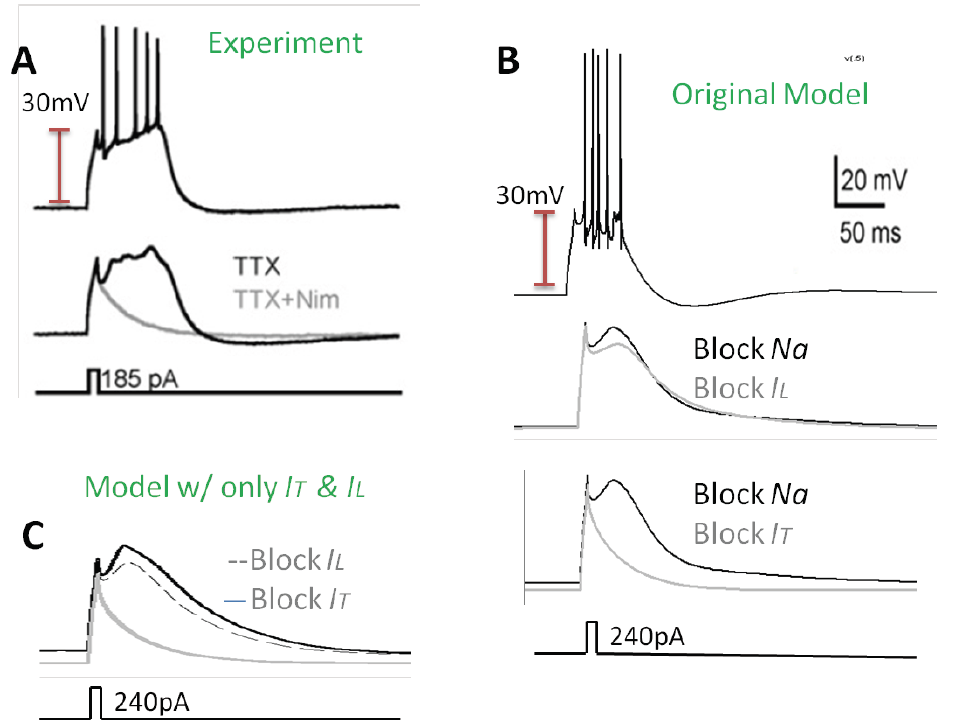
\includegraphics[scale=0.6]{chapters/chapter3/figures/fig1}} + \parbox{10mm}{\centering 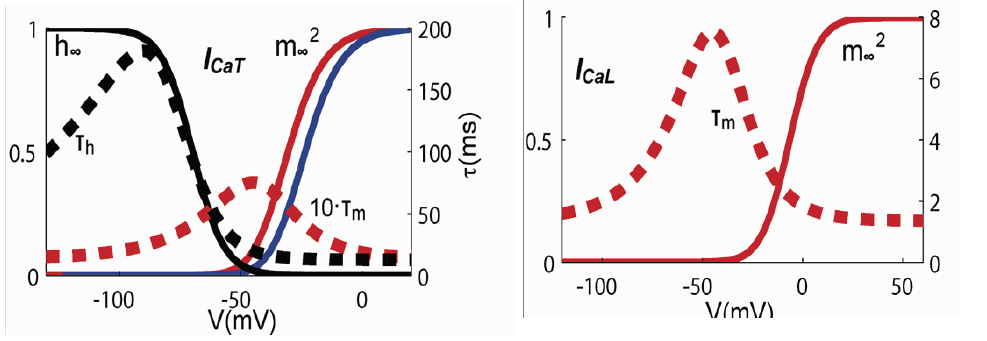
\includegraphics[scale=0.6]{chapters/chapter3/figures/fig2}} + \parbox{10mm}{\centering 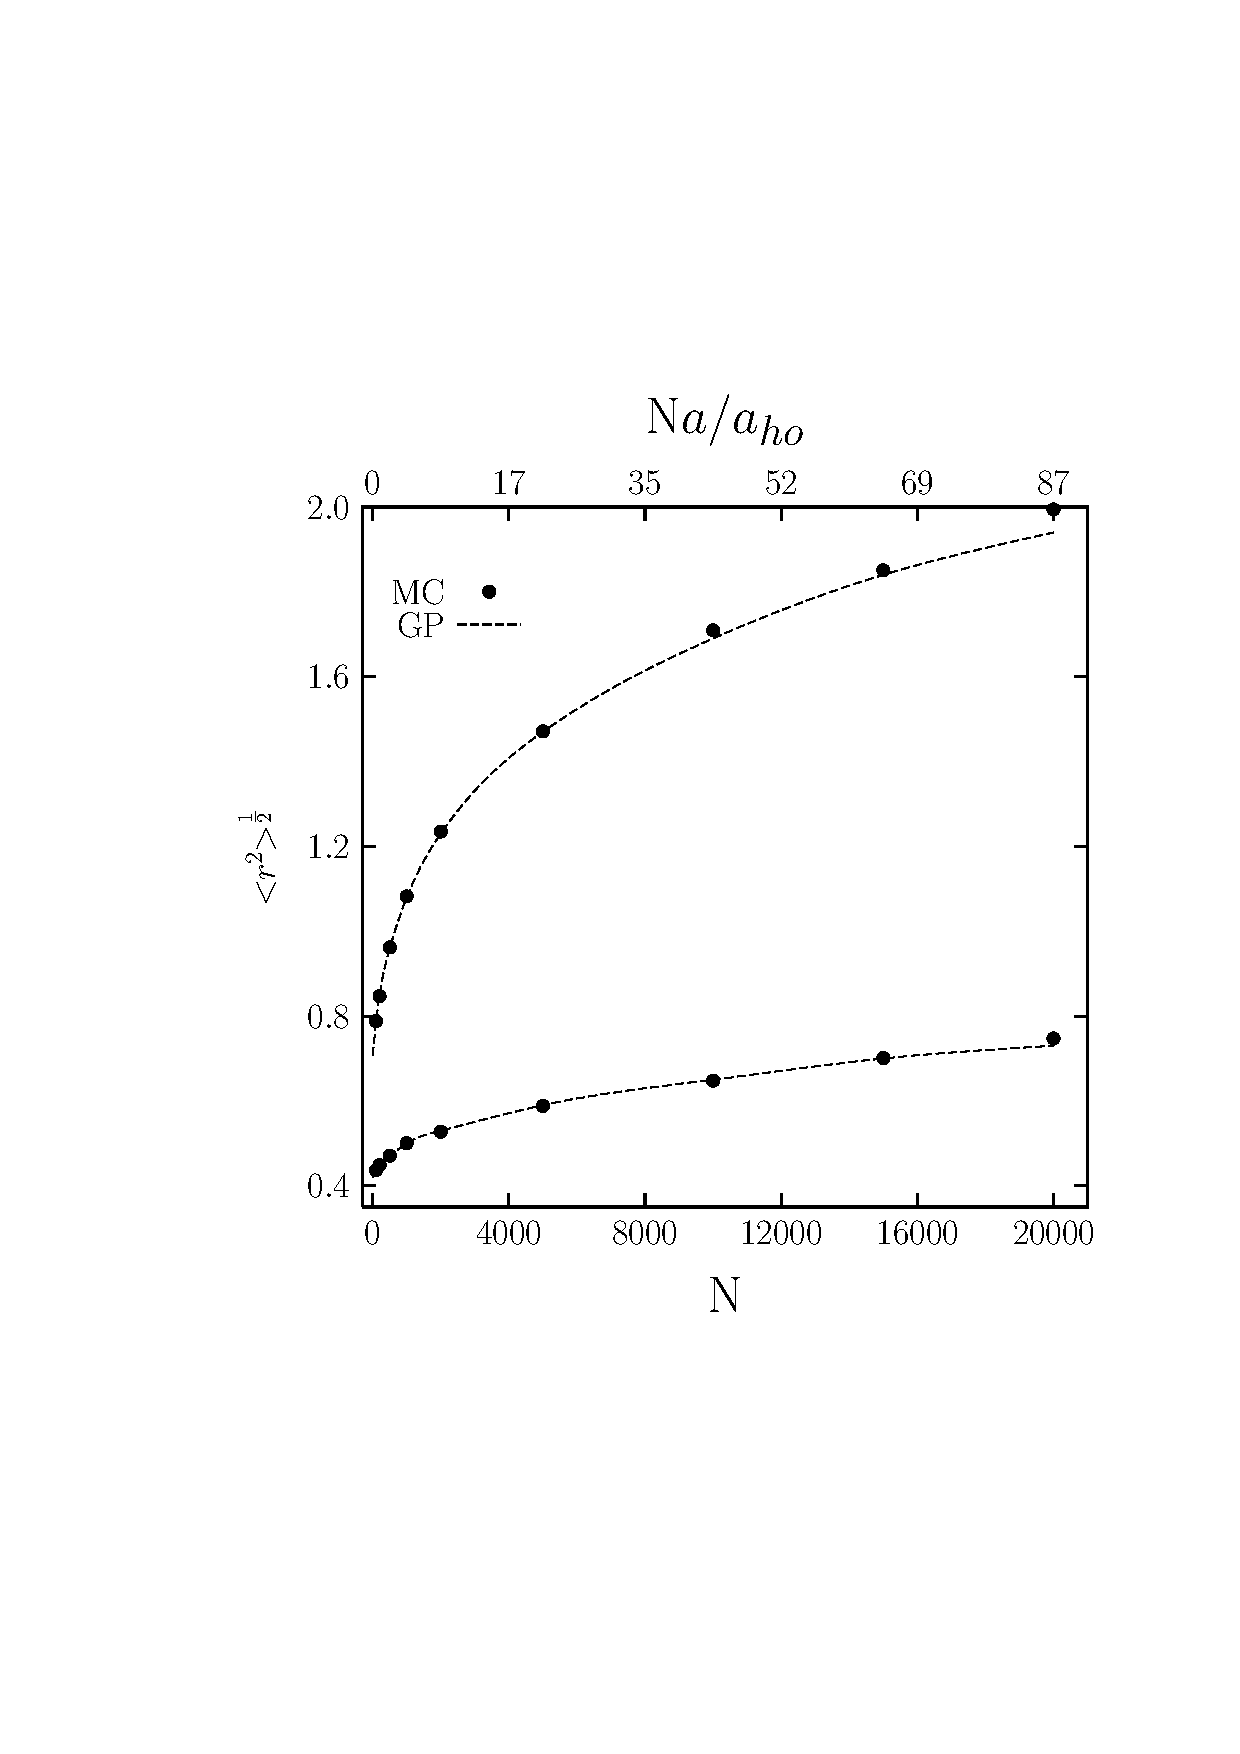
\includegraphics[scale=0.6]{chapters/chapter3/figures/fig3}} + \parbox{10mm}{\centering 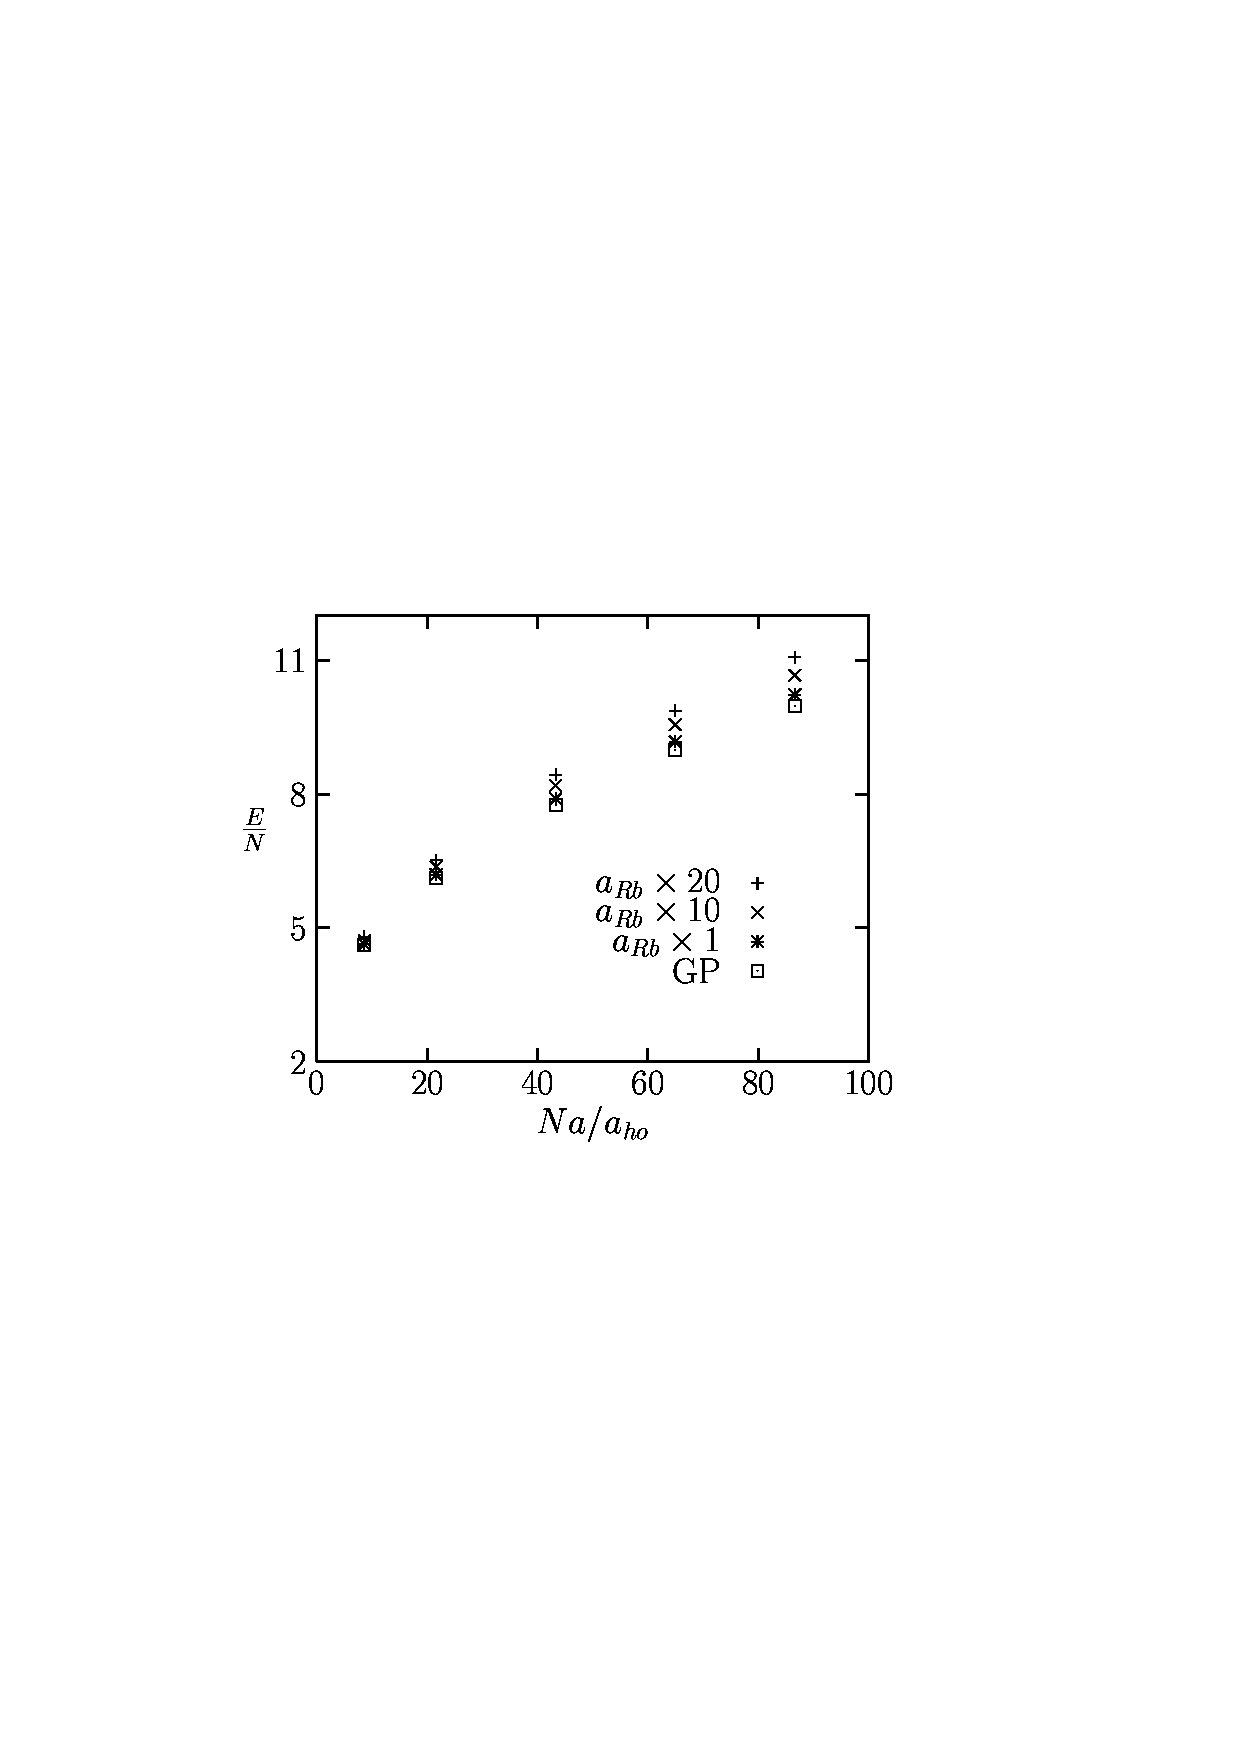
\includegraphics[scale=0.6]{chapters/chapter3/figures/fig4}} + \parbox{10mm}{\centering \includegraphics[scale=0.6]{chapters/chapter3/figures/dot}}  + \parbox{10mm}{\centering 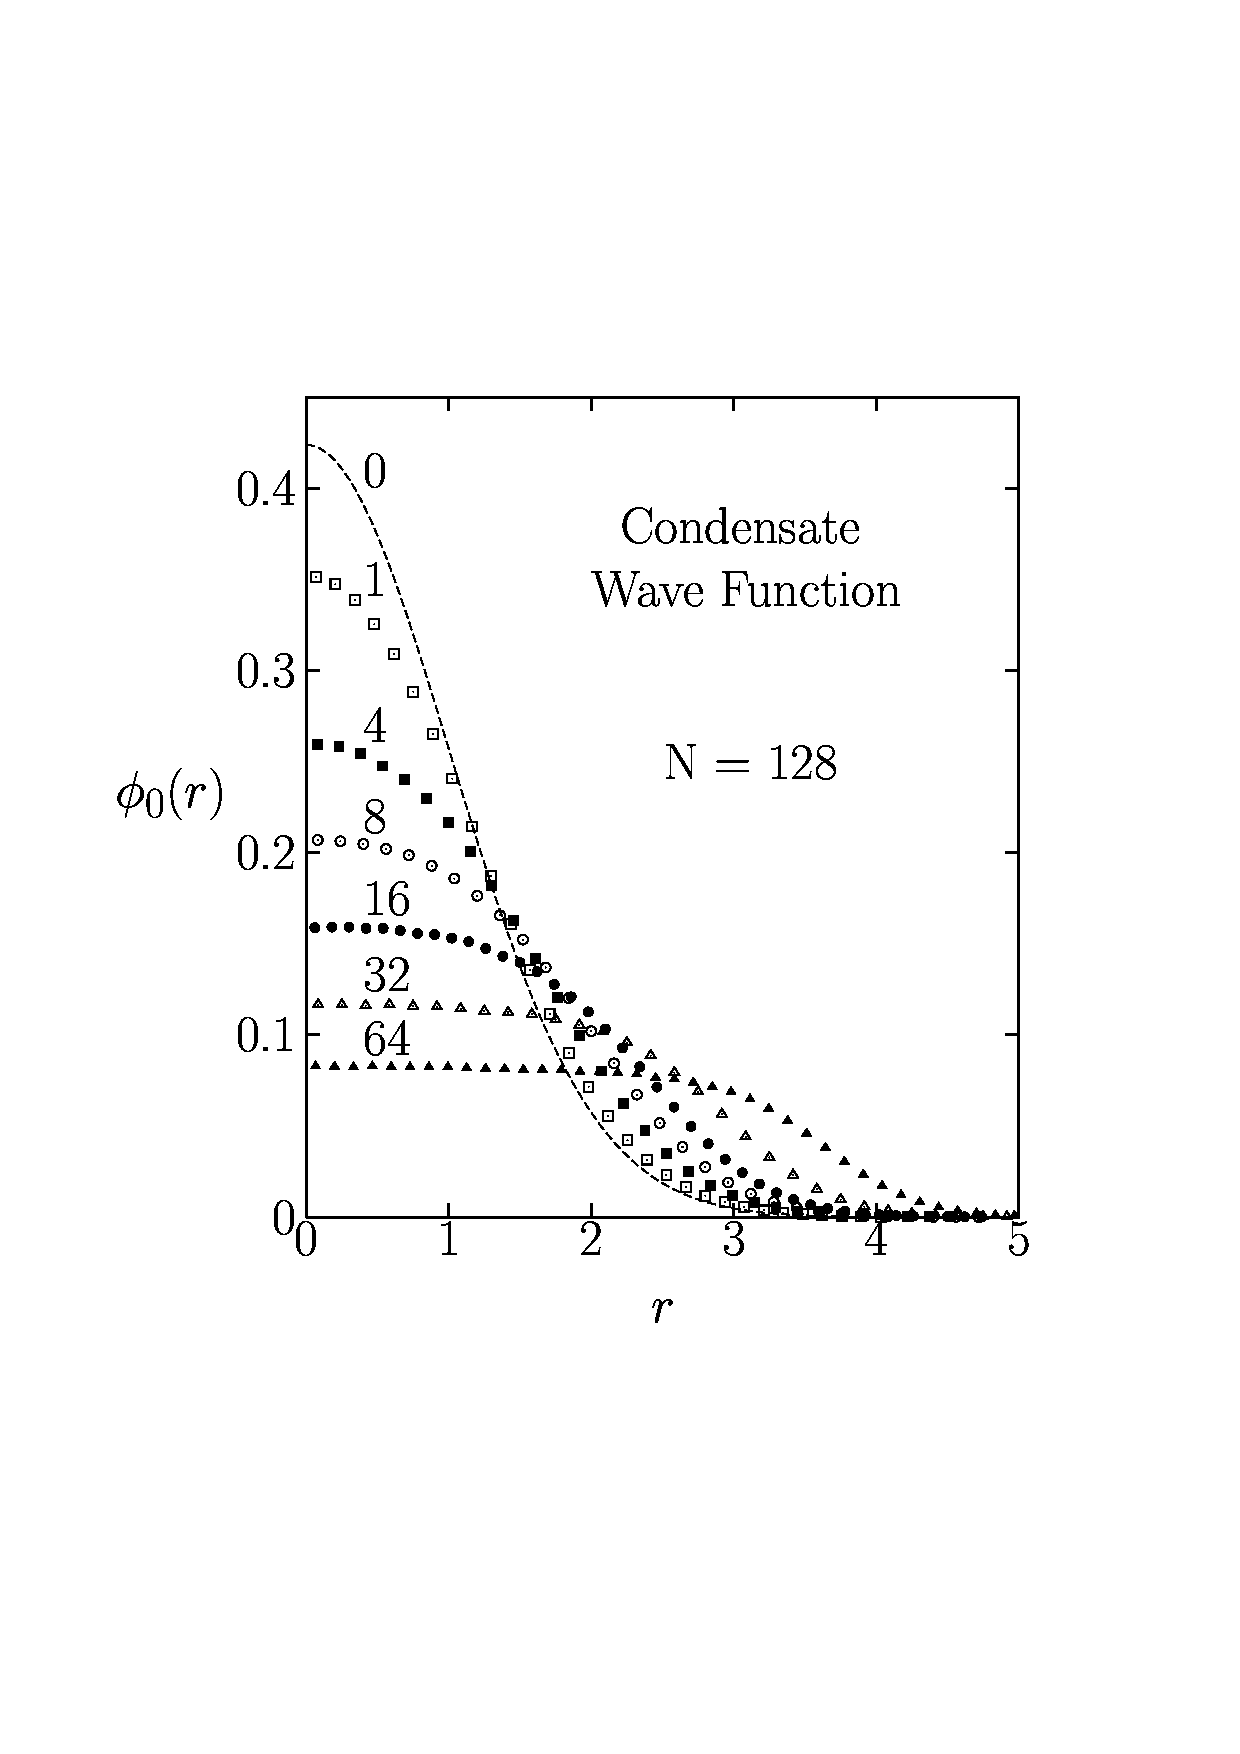
\includegraphics[scale=0.6]{chapters/chapter3/figures/fig5}} + \parbox{10mm}{\centering 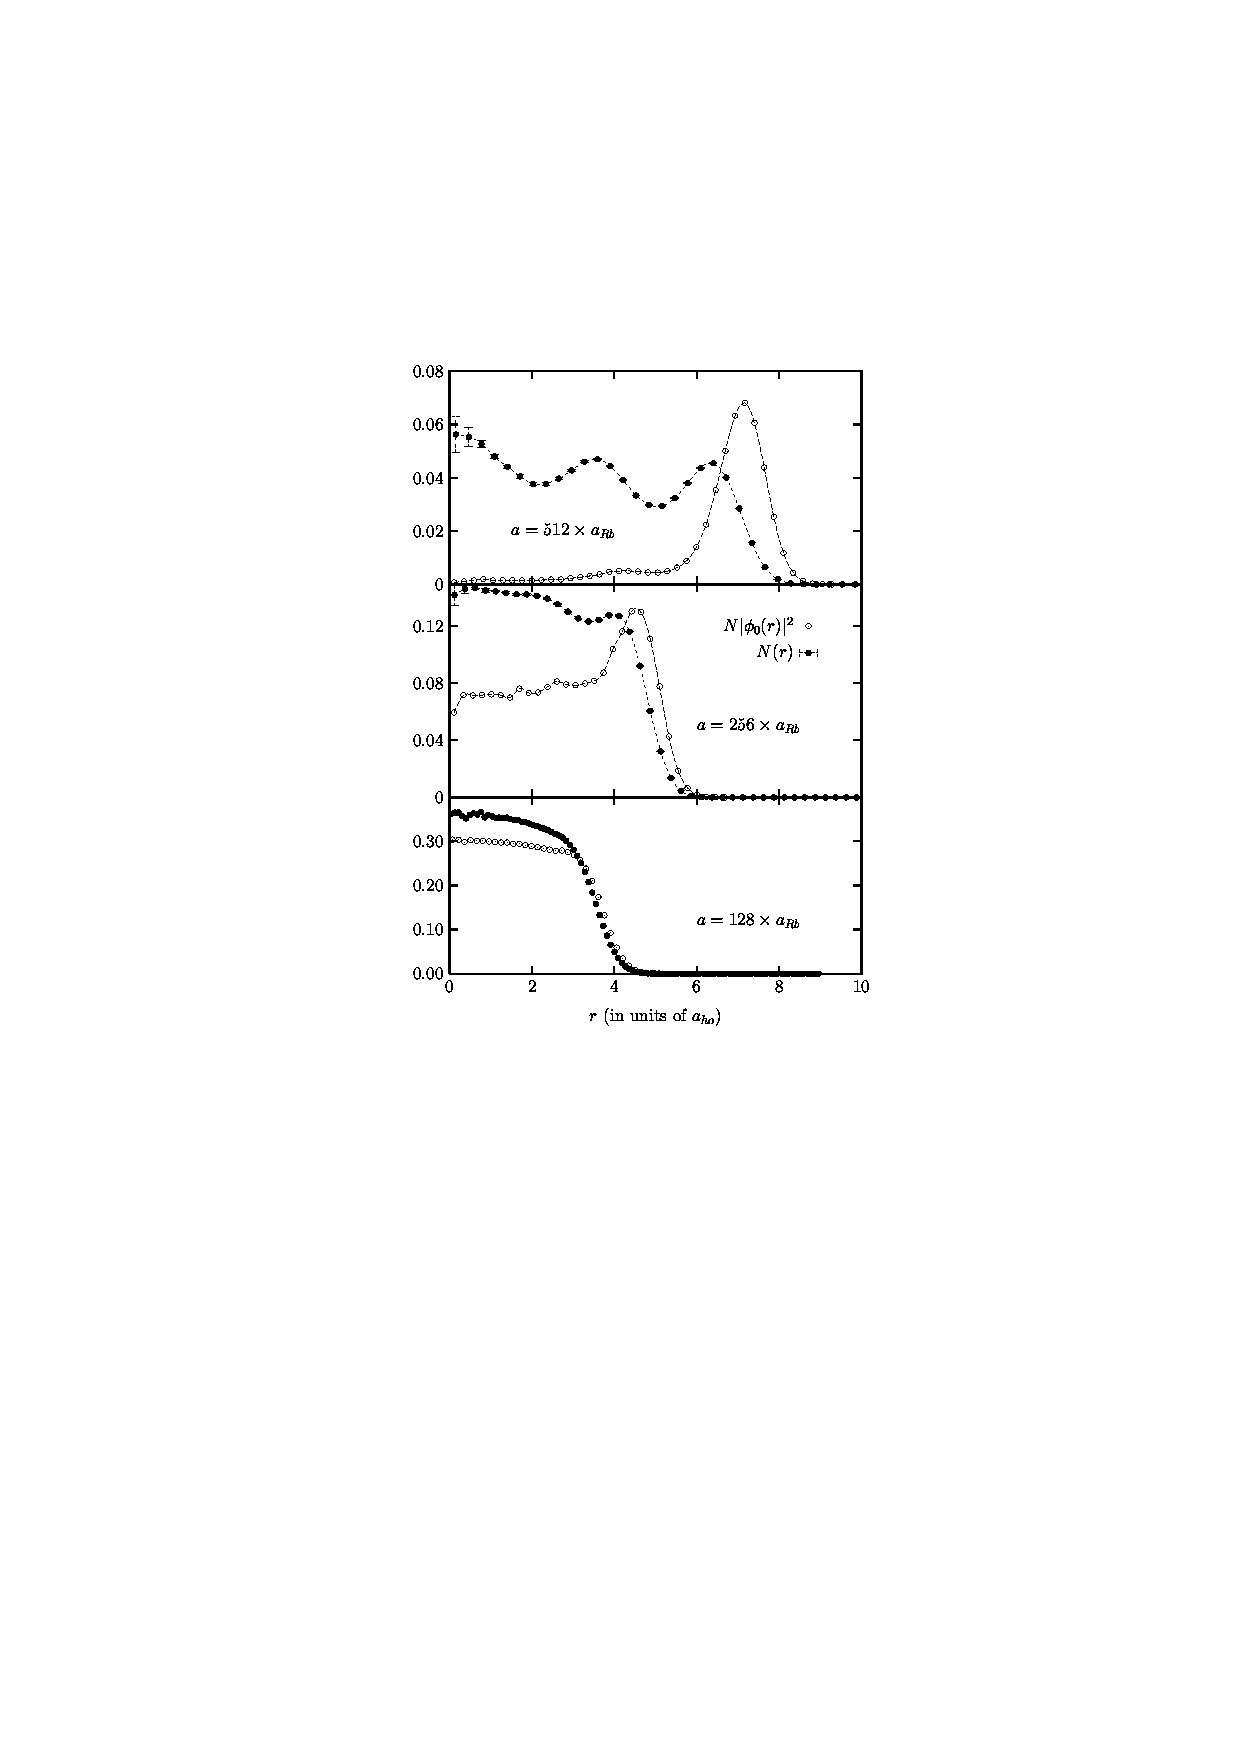
\includegraphics[scale=0.6]{chapters/chapter3/figures/fig6}} + \parbox{10mm}{\centering \includegraphics[scale=0.6]{chapters/chapter3/figures/dot}}  +  \parbox{10mm}{\centering 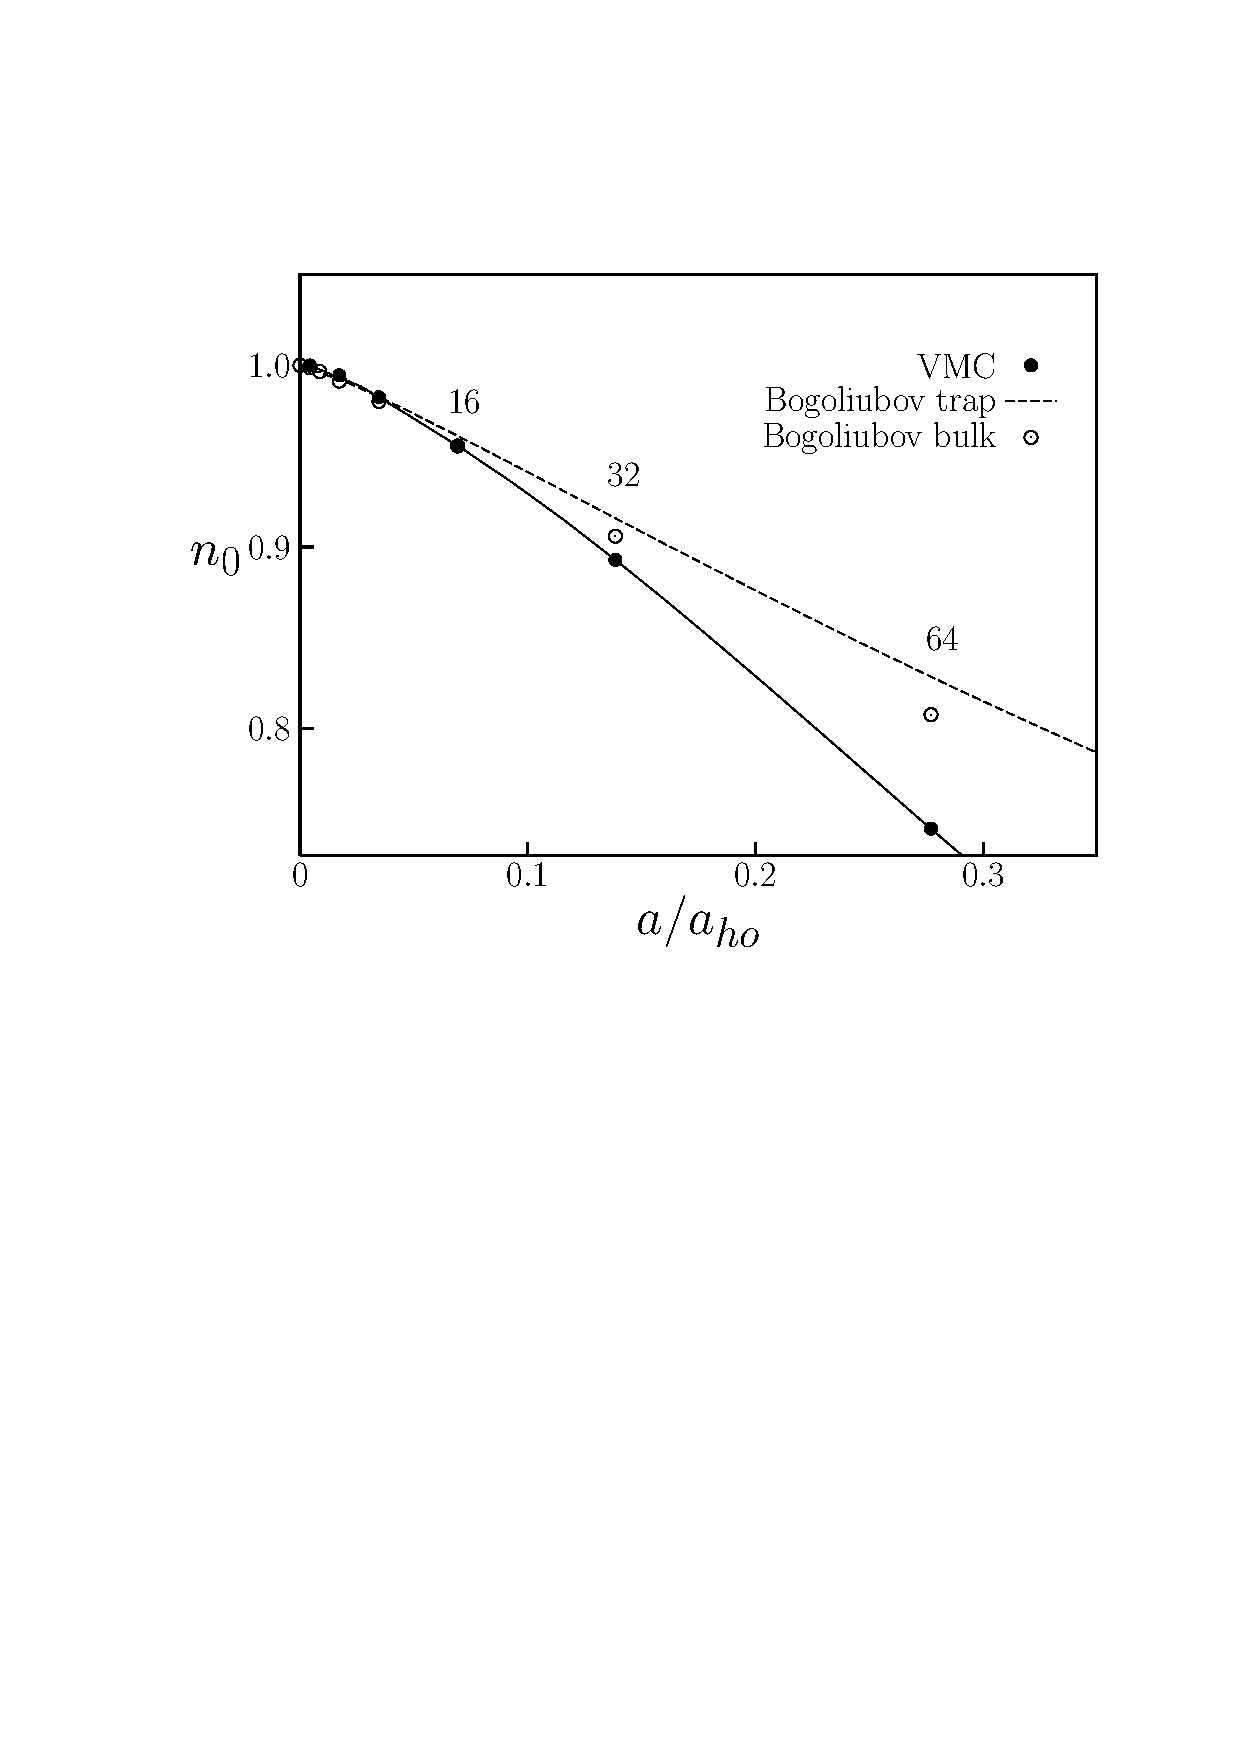
\includegraphics[scale=0.6]{chapters/chapter3/figures/fig7}} + \parbox{10mm}{\centering \includegraphics[scale=0.6]{chapters/chapter3/figures/dot}}\\
\notag
&+ \parbox{10mm}{\centering 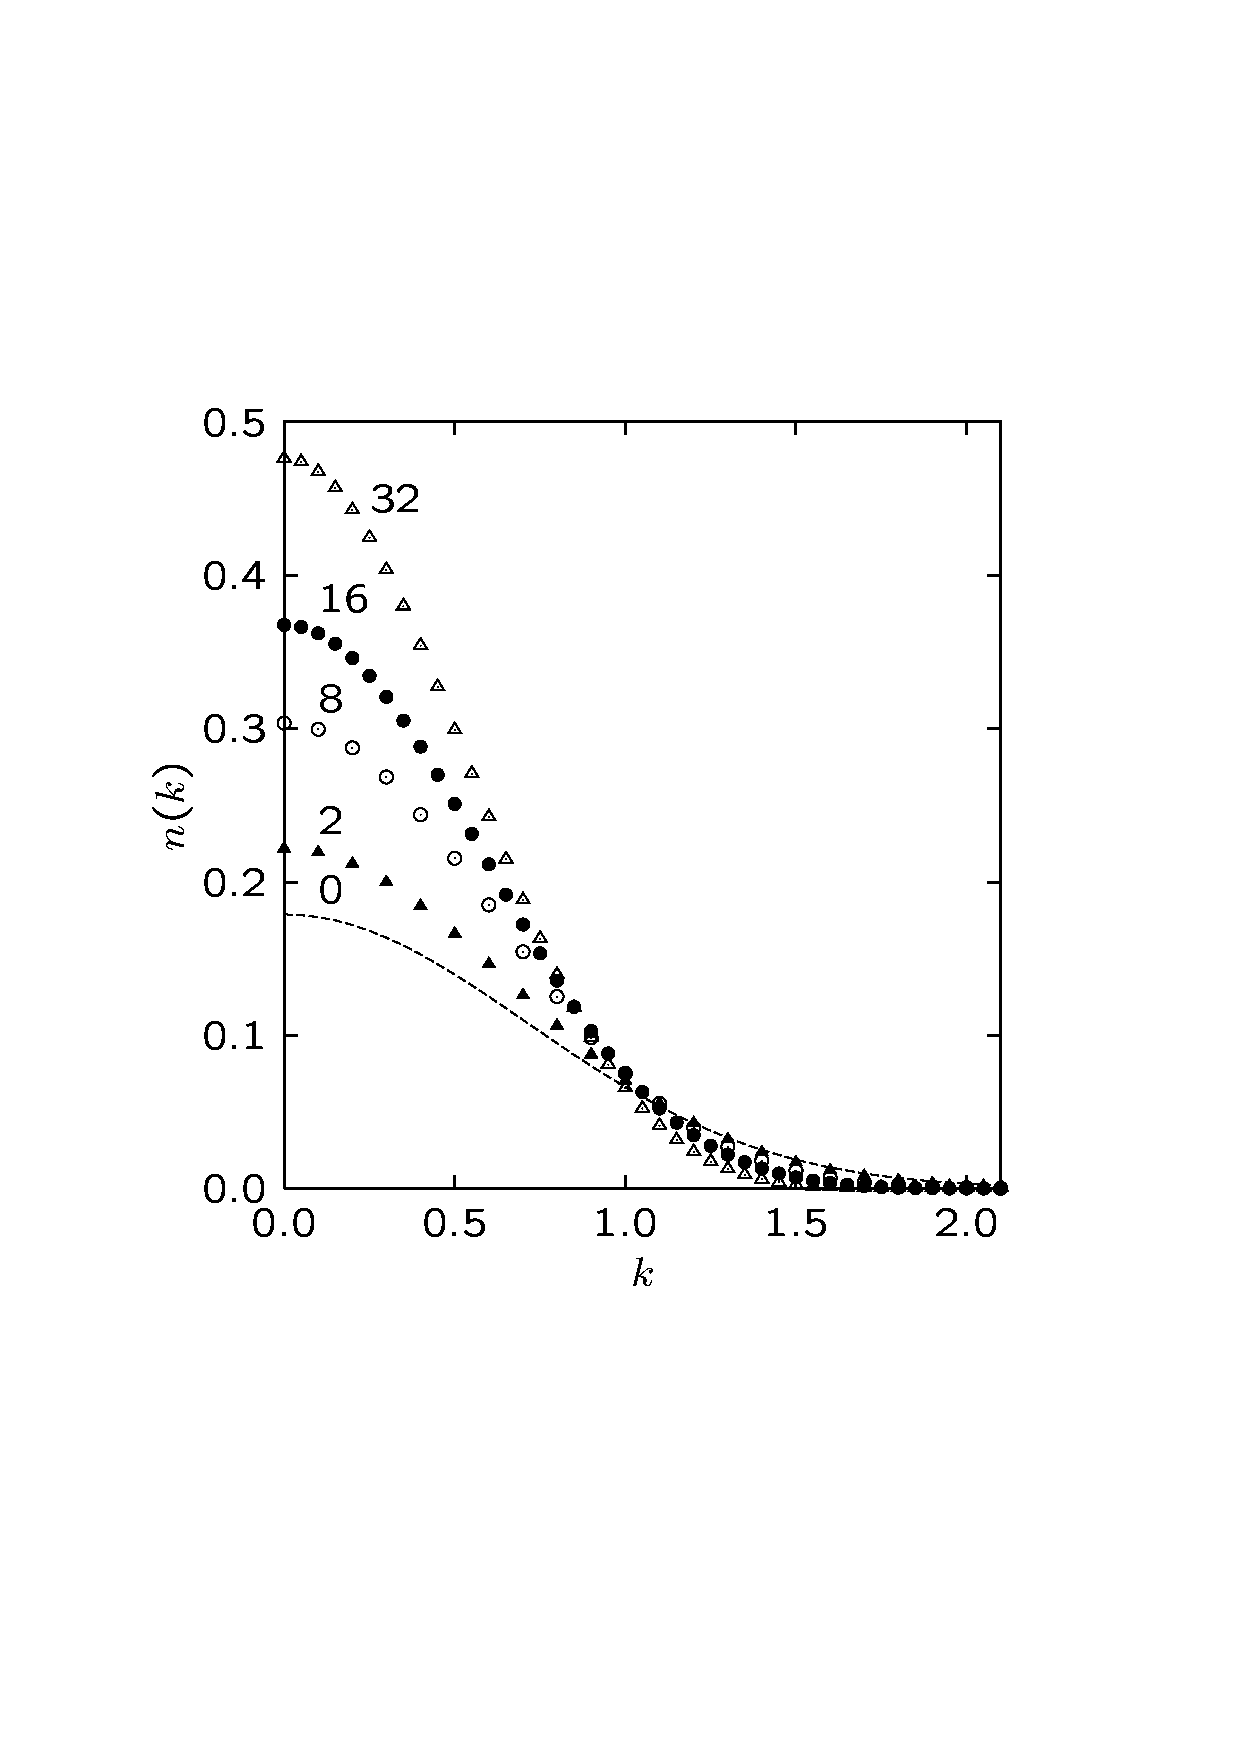
\includegraphics[scale=0.6]{chapters/chapter3/figures/fig9}} + \parbox{10mm}{\centering 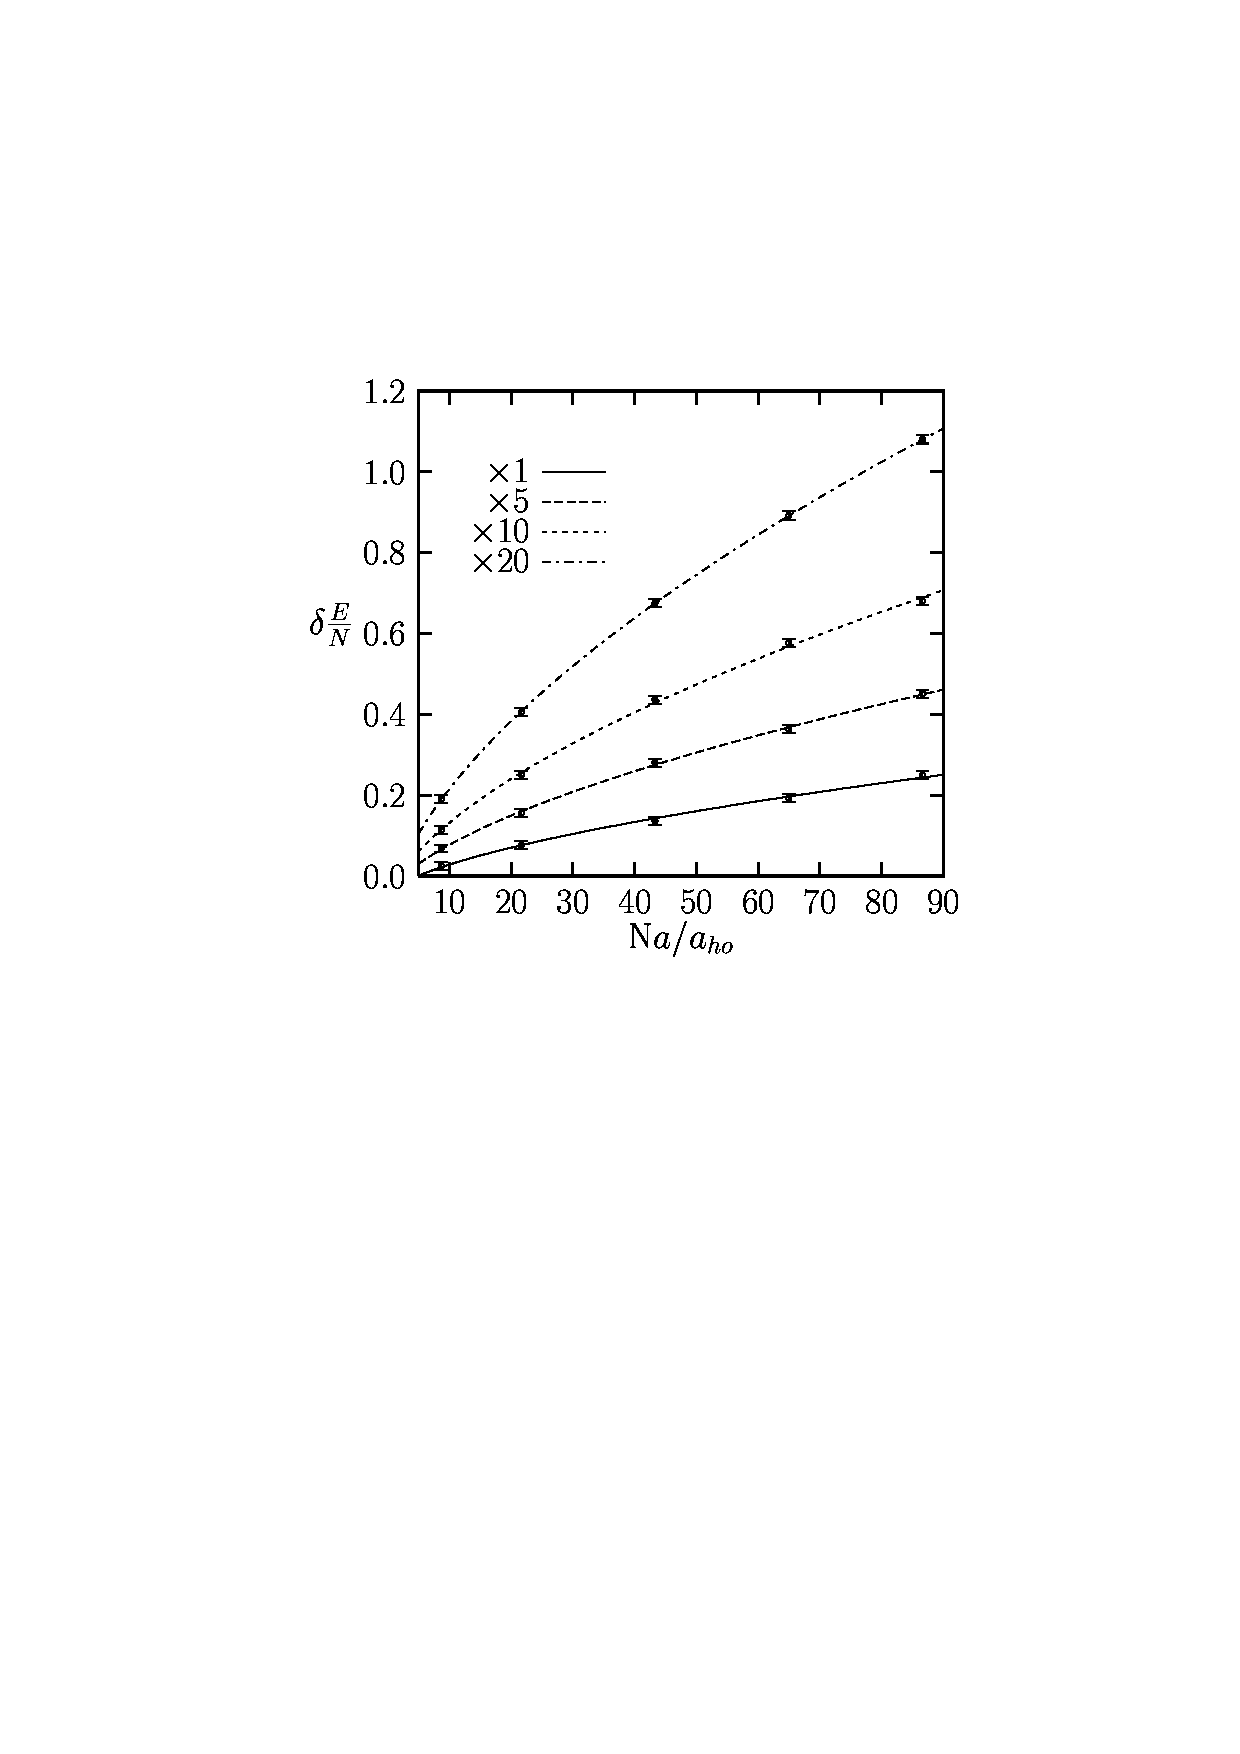
\includegraphics[scale=0.6]{chapters/chapter3/figures/fig10}} + \parbox{10mm}{\centering \includegraphics[scale=0.6]{chapters/chapter3/figures/dot}} + \parbox{10mm}{\centering \includegraphics[scale=0.6]{chapters/chapter3/figures/fig11}} + \parbox{10mm}{\centering \includegraphics[scale=0.6]{chapters/chapter3/figures/dot}} + \parbox{10mm}{\centering \includegraphics[scale=0.6]{chapters/chapter3/figures/fig13}} + \parbox{10mm}{\centering \includegraphics[scale=0.6]{chapters/chapter3/figures/fig14}} + \parbox{10mm}{\centering \includegraphics[scale=0.6]{chapters/chapter3/figures/dot}} + \parbox{10mm}{\centering \includegraphics[scale=0.6]{chapters/chapter3/figures/fig15}} + 
\parbox{10mm}{\centering \includegraphics[scale=0.6]{chapters/chapter3/figures/dot}}   \\
\notag
&+ \parbox{10mm}{\centering \includegraphics[scale=0.6]{chapters/chapter3/figures/fig16}} + \parbox{10mm}{\centering \includegraphics[scale=0.6]{chapters/chapter3/figures/fig17}} + \parbox{10mm}{\centering \includegraphics[scale=0.6]{chapters/chapter3/figures/dot}} + \parbox{10mm}{\centering \includegraphics[scale=0.6]{chapters/chapter3/figures/fig18}} + \parbox{10mm}{\centering \includegraphics[scale=0.6]{chapters/chapter3/figures/dot}} +  \parbox{10mm}{\centering \includegraphics[scale=0.6]{chapters/chapter3/figures/fig19}} + \parbox{10mm}{\centering \includegraphics[scale=0.6]{chapters/chapter3/figures/fig20}} + \parbox{10mm}{\centering \includegraphics[scale=0.6]{chapters/chapter3/figures/dot}} + \parbox{10mm}{\centering \includegraphics[scale=0.6]{chapters/chapter3/figures/fig21}} + \parbox{10mm}{\centering \includegraphics[scale=0.6]{chapters/chapter3/figures/dot}} \\
\notag
&+ \parbox{10mm}{\centering \includegraphics[scale=0.6]{chapters/chapter3/figures/dot}} + \parbox{10mm}{\centering \includegraphics[scale=0.6]{chapters/chapter3/figures/dot}} + \parbox{10mm}{\centering \includegraphics[scale=0.6]{chapters/chapter3/figures/fig22}} + \parbox{10mm}{\centering \includegraphics[scale=0.6]{chapters/chapter3/figures/fig23}} + \parbox{10mm}{\centering \includegraphics[scale=0.6]{chapters/chapter3/figures/fig24}} + \parbox{10mm}{\centering \includegraphics[scale=0.6]{chapters/chapter3/figures/fig25}} + \parbox{10mm}{\centering \includegraphics[scale=0.6]{chapters/chapter3/figures/fig26}} + \parbox{10mm}{\centering \includegraphics[scale=0.6]{chapters/chapter3/figures/dot}} + \parbox{10mm}{\centering \includegraphics[scale=0.6]{chapters/chapter3/figures/fig27}} + \parbox{10mm}{\centering \includegraphics[scale=0.6]{chapters/chapter3/figures/dot}}.
\end{align}
The horizontal lines represents the single-electron basis functions with spin included so that that each orbital can only be occupied by one electron at most. The non-interacting ground state is represented by the shaddowed area with a bold horizontal line denoting the fermie level of the system. The black circles obviously represents electrons, and the white ones represents holes. We will in following denote $n$-particle $n$-hole excitations by the shorthand notation $npnh$-excitations. The $1p1h$-excitations are unique in the sense that given a $1p1h$-excited determinant, we can only achieve this state by one distinct excitation. In the the $2p2h$ case, each excited state can be reached by two different excitations as indicated by the excitation lines. In the general case, one can a produce each $npnh$-excited state by $n!$ different ways of excitations. Physically, however, this is irrelevant since the only important information lies in the occupied single-electron states. Each diagram therefore represents $\textit{one}$ (excited) slater determinant with corresponding expansion coefficient included.  

Given the exact wave function $\ket{\Psi}$ and the complete set of slater determinants, the linear combination in Eq. (\ref{exp: Exact wave function}) is uniquely determined. However, the exact many-body wave function is $\textit{not}$ known, simply because this is the main objective in our calculation. In addition, as stated in chapter \ref{ch: Quantum Mechanics of Many-Body Systems}, the many-body problem can in most cases not be solved exactly. This imply that the infinite sum in Eq. (\ref{exp: Exact wave function}) cannot (necessarily) be determined exactly. At first sight, this does not look promising at all. The fact is, however, that Eq. (\ref{exp: Exact wave function}) serves as a fundamental starting point for several powerful and accurate $\textit{ab initio}$ methods such as configuration interaction (CI) and coupled-cluster (CC). The basic idea is that the exact wave function is approximated with a (necessarily) truncated determinantal expansion, and that the coefficients are determined by the Schr�dinger equation. Information of the electron-electron correlations hence lie in the expansion coefficients. Given the exact wave function one may always in principle tune these cofficients to yield the exact state. However, when the exact wave function is the objective, physical considerations must be build into these coefficients right from the beginning. Different approximations schemes serve as the origin for different many-body methods. Before we turn this point, basic notation are presented. 

%-----------------------
\subsection{Notation}
\label{subsec: Notation}
%-----------------------
We will in the following use the particle-hole formalism presented in section \ref{subsec: Particle-hole formalism}. The reference state is defined as 
\begin{align}
\ket{r} = \ket{\Phi},
\end{align}
where $\ket{\Phi_0}$ is the ground state of the non-interacting electronic system,
\begin{align}
\ket{\Phi_0} = \cre{\alpha_1}\cre{\alpha_2}..\cre{\alpha_N}\ket{0}.
\end{align}
The standard state-subscript from the particle-hole formalism is used; $i$,$j$,$k$,.. denot hole states and $a$,$b$,$c$,.. denote particle states. Hole states are single-electron orbitals that are occupied in the reference state, while particle states are all states beyond the fermi state. These subspaces is called occupied space and virtual space, respectively. States that are in either of the subspaces are denoted $p$,$q$,$r$,... We will not use the standard quasi-particle creation and annihilation operators $\crequasi{\alpha}$ and $\anquasi{\alpha}$ explicitly, but in an implicit way using vacuum creation and annihilation operators with quantum numbers $i,j,..,a,b,..,p,q,..$ indicating in which subspace they act. 
\begin{align}
\cre{i} &= \anquasi{\alpha} \hspace{0.5cm} \alpha\leq\alpha_F\\
\cre{a} &= \crequasi{\alpha} \hspace{0.5cm} \alpha>\alpha_F\\
\an{i} &= \crequasi{\alpha} \hspace{0.5cm} \alpha\leq\alpha_F\\
\an{a} &= \anquasi{\alpha} \hspace{0.5cm} \alpha>\alpha_F
\end{align}
We may now construct particle-, hole- and particle-hole (excited determinants) states by acting with strings of creation and annihilation operators on the reference state,
\begin{align}
\notag
\cre{a}\cre{b}\cre{c}..\ket{\Phi_0} &=  \parbox{10mm}{\centering \includegraphics[scale=0.2]{chapters/chapter3/figures/particleState}}& \hspace{1cm} \an{i}\an{j}\an{k}..\ket{\Phi_0}  &= \parbox{10mm}{\centering \includegraphics[scale=0.2]{chapters/chapter3/figures/holeState}}& \hspace{1cm} \cre{a}\cre{b}\cre{c}.. ..\an{k}\an{j}\an{i}\ket{\Phi_0} &= \parbox{10mm}{\centering \includegraphics[scale=0.2]{chapters/chapter3/figures/holeParticleState}}\\
\notag
&\equiv \ket{\Phi^{abc..}}& &\equiv \ket{\Phi_{ijk..}}& &\equiv \ket{\Phi_{ijk..}^{abc..}}
\end{align}
As shown above, particle-states will be denoted with virtual orbitals on the top right position of the state, hole-states with ocuupied orbitals in the lower right position, and particle-hole states with both virtual states and occupied states at their respective positions. The number of occupied and virtual orbitals yield the number of electrons in the system. For example, 
\begin{align}
\ket{\Phi_{n_o}^{n_v}},
\end{align}
represents a $(N+n_v-n_o)$-particle state, where $N$ is the number of particles in the reference state. When $n_v = n_o \neq 0$, the state represents an excitation of the reference state. 

%--------------------------------------------------------------------------------------------------------------------------------------------------------------
\section{Fundamental concepts}
\label{sec: fundamental concepts}
%--------------------------------------------------------------------------------------------------------------------------------------------------------------
We are seeking the solution of the Schr�dinger equation 
\begin{align}
\label{exp: Exact electronic Schr�dinger equation}
\OP{H}\ket{\Psi} = E\ket{\Psi},
\end{align}
for a system of $N$ interacting electrons in an external potential $u$. The hamiltonian written in second quantization (see section \ref{sec: Second Quantization}) reads 
\begin{align}
\label{exp: Electronic hamiltonian on second quantized form}
\OP{H} = \sum_{pq} \for{p}{h}{q} \cre{p}\an{q} + \frac{1}{4} \sum_{pqrs}\for{pq}{v}{rs}\cre{p}\cre{q}\an{s}\an{r},
\end{align}
where the two-body interaction elements are antisymmetrized. The one-body hamiltonian
\begin{align}
\label{exp: One-body hamiltonian}
\OP{h} = \OP{t} + \OP{u},
\end{align}
where $\OP{t}$ is the kinetic energy and $\OP{u}$ is the external one-body potential. The two-body interaction,
$\OP{v}$, is the well-known Coulomb interaction.

The many-electron problem can in general not be solved exactly, which imply that the energy eigenfunctions cannot be
written down in an analytically closed form. However, as pointed out in the introduction to this chapter, given an 
arbitrary orthonormal and complete set of single-electron functions, the exact energy
eigenfunctions can be expanded in an infinite series (\ref{exp: Exact wave function}) of slater determinants constructed from these. We choose the
single-electron basis to be the set of energy eigenfunctions determined by the single-particle Schr�dinger equation
\begin{align}
\OP{h}\ket{\phi_\alpha} = \epsilon_\alpha \ket{\phi_\alpha},
\end{align}
with $\OP{h}$ defined in Eq. (\ref{exp: One-body hamiltonian}). Hence, according to Eq. (\ref{exp: Exact wave function}) 
and the schematic drawing in Eq. (\ref{exp: Exact wave function, schematic drawing}), the exact wave function can be 
written as a linear combination of all possible exciations (energy eigenstates) of the non-interacting system. Applying the
notation presented in the previous chapter, Eq. (\ref{exp: Exact wave function}) reads
\begin{align}
\label{exp: Exact wave function, new notation}
\ket{\Psi} = C_0\ket{\Phi} + \sum_{ia}C_i^a\ket{\Phi_i^a} + \sum_{ijab}C_{ij}^{ab}\ket{\Phi_{ij}^{ab}} + ... + 
\sum_{ijk..abc..}C_{ijk..}^{abc..}\ket{\Phi_{ijk..}^{abc..}},
\end{align}
where the infinite series of determinantal functions naturally terminates when all particles are excited. The first sum
represents $1p1h$-excitations, the second $2p2h$-exciations, and so forth up to $NpNh$-excitations. Even though the 
expansion is finite in order of particle-hole excitations, it is still infinite in the virtual orbitals $a,b,c..$. If we 
were able to go to infinity in the virtual orbitals, the exact wave function is given by Eq. (\ref{exp: Exact wave function, new notation}).
However, Eq. (\ref{exp: Exact wave function, new notation}) is not complete in the sense that it does not give any 
information about what contributes to the individual expansion coefficients. It simply tell us that given the exact
wave function we can in principle always tune each coefficient iteself without explicitly calculating its different contributions, 
so that the linear expansion of determinantal functions yield the exact state. The wave function is however $\textit{not}$ known, which imply that the coefficients are the unknowns to be determined by the Schr�dinger equation. Before this can be done, we must specify what contributes to each expansion coefficients $C_{ij..}^{ab..}$. For a given excited slater determinant $\ket{\Phi_{ij..}^{ab..}}$, the corresponding expansion coefficients $C_{ij..}^{ab..}$ gets contributions from $\textit{excitation amplitudes}$ with all possible electron-electron correlation. As an example, consider the $3p3h$-excited determinant $\ket{\Phi_{ijk}^{abc}}$. The corresponding expansion coefficient $C_{ijk}^{abc}$ gets contributions from excitation amplitudes with all possible electron-electron ,
\begin{align}
C_{ijk}^{abc} = t_i^at_j^bt_k^c + t_{ij}^{ab}t_k^c + t_i^at_{jk}^{bc} + t_j^bt_{ik}^{ac} + t_{ijk}^{abc}
\end{align}
The coupling can shematically be shown by,
\begin{align}
C_{ijk}^{abc}\ket{\Phi_{ijk}^{abc}} &= \pr{t_i^at_j^bt_k^c + t_{ij}^{ab}t_k^c + t_i^at_{jk}^{bc} + t_j^bt_{ik}^{ac} + t_{ijk}^{abc}}\ket{\Phi_{ijk}^{abc}} \\ 
\label{exp: Expansion coefficients coupling}
&=
\parbox{10mm}{\centering \includegraphics[scale=0.2]{chapters/chapter3/figures/particleCoupling}} + 
\parbox{10mm}{\centering \includegraphics[scale=0.2]{chapters/chapter3/figures/particleCoupling2}} + 
\parbox{10mm}{\centering \includegraphics[scale=0.2]{chapters/chapter3/figures/particleCoupling3}} + 
\parbox{10mm}{\centering \includegraphics[scale=0.2]{chapters/chapter3/figures/particleCoupling4}} +
\parbox{10mm}{\centering \includegraphics[scale=0.2]{chapters/chapter3/figures/particleCoupling5}}.
\end{align}
Each the figures in Eq. (\ref{exp: Expansion coefficients coupling}) denote the contribution to the total expansion coefficient $C_{ijk}^{abc}$ from one of the possible correlations of electrons within specific orbitals. The first figure in Eq. (\ref{exp: Expansion coefficients coupling}) represents the excited slater determinant with three $1p1h$-excitation amplitudes that do not couple any of the electrons. This is a crucial contribution when we consider a system consisting of two subsystems that do not interact with each other. In addition, a weakly interacting system may get important contribution to the $3p3h$ from $3$ independent $1p1h$-excitations. The second, third and forth term in Eq. (\ref{exp: Expansion coefficients coupling}) denote the excited determinant where the motions of two electrons within selected pair of orbitals are correlated. The fifth term represents the contribution the expansion coefficient where all electrons are coupled. This example illustrates that for a given $npnh$-excited slater determinant, one may produce this state by correlating the motion of electrons within specific orbitals in all possible ways. The corresponding expansion coefficient hence gets contributions from excitation amplitudes with all possible electron-electron coupling. 

We now define the single-orbital excitation operator (cluster operator)
\begin{align}
\OP{t}_i = \sum_a t_i^a \cre{a}\an{i},
\end{align}
which acting on the reference state yields,
\begin{align}
\OP{t}_i\ket{\Phi} = \sum_a t_i^a \ket{\Phi_i^a}. 
\end{align}
Similarly, we define the two-orbital excitation operator, which couple the pair of excited electrons, as
\begin{align}
 \OP{t}_{ij}^{ab} = \frac{1}{2}\sum_{ab}t_{ij}^{ab}\cre{a}\cre{b}\an{j}\an{i},
\end{align}
which acting on the reference state yields 
\begin{align}
\OP{t}_{ij}^{ab}\ket{\Phi} = \frac{1}{2}\sum_{ab}t_{ij}^{ab}\ket{\Phi_{ij}^{ab}},
\end{align}
where the motion of the excited pair of electrons are correlated. In general case, the $n$-orbital excitation operator is defined as
\begin{align}
\OP{t}_{ijk..}^{abc..} = \frac{1}{n!}\sum_{abc..}t_{ijk..}^{abc..}\cre{a}\cre{b}\cre{c}....\an{k}\an{j}\an{i}.
\end{align}
When acting on the reference state it produces all $npnh$-excitations (with holes in i,j,k,..) where the motions of all excited electrons are correlated with each other,
\begin{align}
\OP{t}_{ijk..}^{abc..}\ket{\Phi} = \frac{1}{n!}\sum_{abc..}t_{ijk..}^{abc..}\ket{\Phi_{ijk..}^{abc..}}. 
\end{align}
These excitation operators allow us to produce excited determinants with all possible electron-electron coupling. For example, 
\begin{align}
\pr{\OP{t}_i\OP{t}_j + \OP{t}_{ij}}\ket{\Phi} = \frac{1}{2}\sum_{ab}\pr{t_i^at_j^b + t_{ij}^{ab}}\ket{\Phi_{ij}^{ab}},
\end{align}
produces all $2p2h$-excited determinants with a hole-pair in $i$ and $j$. In addition, by summing over $i$ and $j$, we obtain all $2p2h$-states
\begin{align}
\frac{1}{4}\sum_{ijab}\pr{t_i^at_j^b + t_{ij}^{ab}}\ket{\Phi_{ij}^{ab}}.
\end{align}
It is therefore appropriate to define $\textit{total}$ excitation amplitudes,
\begin{align}
\OP{T}_1 &\equiv \sum_i \OP{t}_i = \sum_{ia}t_i^a\cre{a}\an{i}\\
\OP{T}_2 &\equiv \frac{1}{2}\sum_{ij}\OP{t}_{ij}^{ab} = \frac{1}{4}\sum_{ijab}t_{ij}^{ab}\cre{a}\cre{b}\an{j}\an{i}\\
\notag
&\vdots \hspace{1cm} \vdots \\
\OP{T}_n &\equiv \frac{1}{n!}\sum \OP{t}_{ijk..}^{abc..}\cre{a}\cre{b}\cre{c}....\an{k}\an{j}\an{i} =  \pr{\frac{1}{n!}}^2\sum_{ijk..abc..}t_{ijk..}^{abc..}\cre{a}\cre{b}\cre{c}....\an{k}\an{j}\an{i}.
\end{align}
The total excitation amplitudes can be used to obtain all-order excitations with all possible coupling between the electrons. For example, all $3p3h$-excitations is obtained by using combining $\OP{T}_1$, $\OP{T}_2$ and $\OP{T}_3$,
\begin{align}
\ket{3p3h} = \pr{\frac{1}{6}\OP{T}_1^3 + \OP{T}_1\OP{T}_2 + \OP{T}_3}\ket{\Phi_0}. 
\end{align}
In the general case, all $npnh$-excitations with all possible correlations are generated by combining $\OP{T}_1$, $\OP{T}_2$, ..., $\OP{T}_n$. 

We can now rewrite the exact wavefunction (\ref{exp: Exact wave function, new notation}) in terms of total excitation operators. It is at this point the difference between configuration interaction and coupled-cluster appears. The configuration interaction method builds up the wavefunction with only fully correlated electrons, i.e. no products of excitation excitation operators. The CI wavefunction reads
\begin{align}
\ket{\Psi}_{CI} = \pr{1 + \OP{T}_1 + \OP{T}_2 + \OP{T}_3 + ... + \OP{T}_N}\ket{\Phi_0}.
\end{align}
The coupled-cluster method, however, also include products of excitation operators, so that the CC wavefunction is given by
\begin{align}
\label{exp: Coupled-cluster wavefunction}
\ket{\Psi}_{CC} &= \Big(1 + \OP{T}_1 + \fpr{\frac{1}{2!}\OP{T}_1^2 + \OP{T}_2} + \fpr{\frac{1}{3!}\OP{T}_1^3 + \OP{T}_1\OP{T}_2 + \OP{T}_3}\\ &+ \fpr{\frac{1}{4!}\OP{T}_1^4 + \frac{1}{2!}\OP{T}_1^2\OP{T}_2 + \OP{T}_1\OP{T}_3 + \frac{1}{2!}\OP{T}_2^2 + \OP{T}_4} + ... + \fpr{... + \OP{T}_N}\Big)\ket{\Phi}.
\end{align}
Higher-order terms (like $\OP{T}_{N+1}$) do not appear since $N$ is the number of electrons in the system. Because all excitation operators commute, all terms in Eq. (\ref{exp: Coupled-cluster wavefunction}) match those from the power series expansion of an exponental function. Thus, the $\textit{exact}$ wavefunction can be written as
\begin{align}
\label{exp: Coupled-cluster wavefunction 2}
\ket{\Psi} = e^{\OP{T}}\ket{\Phi},
\end{align}
where 
\begin{align}
\label{exp: Excitation operators}
\OP{T} = \OP{T}_1 + \OP{T}_2 + ... + \OP{T}_N.
\end{align}
The wavefunction in Eq. (\ref{exp: Coupled-cluster wavefunction 2}) is usually called the $\textit{coupled-cluster wavefunction}$ or the $\textit{exponential ansatz}$. In practical calculations we are obviously forced to choose a model space $\mathcal{P} \subset \mathcal{H}_N$, which is equivalent to truncate the summations in the excitation amplitudes in a specific way. In addition, when the system consists of many particles, we are often forced to truncate the total excitation operator $\OP{T}$ in Eq. (\ref{exp: Excitation operatxcitation operators}). Both the way we choose our model space $\mathcal{P}$ and where we truncate the total excitation operator $\OP{T}$ have consequences for our calculations. At this point, we just emphasize that in practical calculations, the $\textit{exact}$ wavefunction 
\begin{align}
\ket{\Psi} \neq e^{\OP{T}}\ket{\Phi}.
\end{align}
We therefore define the $\textit{coupled-cluster wavefunction}$ as
\begin{align}
\ket{\Psi}_{CC} \equiv e^{\OP{T}}\ket{\Phi},
\end{align}
where 
\begin{align}
\OP{T} = \OP{T}_1 + \OP{T}_2 + ... + \OP{T}_i \hspace{1cm} i\leq N.
\end{align}
This is an $\textit{ansatz}$ to the exact wavefunction. Our hope is that most of the correlations in the system are baked into the coupled-cluster wavefunction so that
\begin{align}
\ket{\Psi} \approx \ket{\Psi}_{CC}.
\end{align}
How ``good'' our coupled-cluster ansatz is, are completely determined by our model space $\mathcal{P}$ and where the total excitation operator $\OP{T}$ is truncated. Truncation at specific excitation level leads to a hierarchy of basic coupled-custer schemes,
\begin{align}
\OP{T} &= \OP{T}_1 + \OP{T}_2 \rightarrow CCSD\\
\OP{T} &= \OP{T}_1 + \OP{T}_2 + \OP{T}_3 \rightarrow CCSDT\\
\OP{T} &= \OP{T}_1 + \OP{T}_2 + \OP{T}_3 + \OP{T}_4 \rightarrow CCSDTQ\\
\notag
\OP{T} &= \OP{T}_1 + \OP{T}_2 + \OP{T}_3 + \OP{T}_4 + ... + \OP{T}_N \rightarrow CCSDTQ..N
\end{align}
where $S$, $D$, $T$ and $Q$ denote single-, double-, triple- and quadruple-excitations, respectively. In the next section, the formal theory of coupled-cluster is presented. 

%------------------------------------------------------------------------------------------------------------------------------------------------------
\section{The formal coupled-cluster theory}
\label{sec: the formal coupled-cluster theory}
%------------------------------------------------------------------------------------------------------------------------------------------------------
The coupled-cluster wavefunction given in Eq. (\ref{exp: Coupled-cluster wavefunction 2}) is the starting point for all CC calculations. First we approximate the exact wavefunction with the CC wavfunction,
\begin{align}
\ket{\Psi} \approx \ket{\Psi}_{CC} = e^{\OP{T}}\ket{\Phi},
\end{align}
which hopefully, but not a priori, is a good approximation. We now substitute the coupled-cluster wavefunction into the Schr�dinger equation, yielding
\begin{align}
\label{exp: Coupled-cluster schr�dinger equation}
\OP{H}e^{\OP{T}}\ket{\Phi} = Ee^{\OP{T}}\ket{\Phi},
\end{align}
where $E$ is the energy eigenvalue. The unknowns are the excitation amplitudes ($t_i^a t_{ij}^{ab}..t_{ijk..}^{abc..}$) and the energy $E$, which are determined by Eq. (\ref{exp: Coupled-cluster schr�dinger equation}). The basic CC equations are the so-called $\textit{energy equation}$ and the $\textit{amplitude equations}$, which constitute the basic CC machinery. The formal form of the equations is found be using a ``projective'' technique where Eq. (\ref{exp: Coupled-cluster schr�dinger equation}) is projected down on an eigenstate of the non-interacting system. The energy equation is found by multiplying the equation with the dual reference state from the left, yielding 
\begin{align}
\label{exp: Formal CC energy equation}
\for{\Phi}{\OP{H}e^{\OP{T}}}{\Phi} = E\for{\Phi}{e^{\OP{T}}}{\Phi} = E.
\end{align}
The last equality in Eq. (\ref{exp: Formal CC energy equation}) follows from the fact that $\indre{\Phi}{\Psi}_{CC} = 1$, by construction. Expressions for the excitation amplitudes is obtained in a similar fashion by left-projecting the Schr�dinger equation down on the excited determinants produced when $\OP{T}$ acts on the reference state,
\begin{align}
\label{exp: Formal CC amplitude equation}
\for{\Phi_{ijk..}^{abc..}}{\OP{H}e^{\OP{T}}}{\Phi} = E\for{\Phi_{ijk..}^{abc..}}{e^{\OP{T}}}{\Phi} = Et_{ijk..}^{abc..}.
\end{align}
Due to the presence of $e^{\OP{T}}$, each amplitude equation for a specific $t_{ijk..}^{abc..}$ couple the amplitude to other excitation amplitudes. The CC equation must therefore be solved iteratively. Again we emphasize that the equations are formally $\textit{exact}$. When $\OP{T}$ is not truncated, the exact wavefunction within our model space $\mathcal{P}$ may be found. 

Eq. (\ref{exp: Formal CC energy equation}) and Eq. (\ref{exp: Formal CC amplitude equation} serves only as a way to get formal insight into the CC method. In practical computer implementation, however, they are not useful \cite{Schaefer}. The first step to obtain programable equations is to multiply Eq. (\ref{exp: Coupled-cluster schr�dinger equation}) with $e^{-\OP{T}}$ from the left, and the use the ``projective'' technique. The modified energy and amplitude equations reads
\begin{align}
\label{exp: Conventional CC energy equation}
\for{\Phi}{e^{-\OP{T}}\OP{H}e^{\OP{T}}}{\Phi} &= E\\
\label{exp: Conventional CC amplitude equation}
\for{\Phi_{ijk..}^{abc..}}{e^{-\OP{T}}\OP{H}e^{\OP{T}}}{\Phi} &= 0,
\end{align}
where the projection onto the excited determinant $\ket{\Phi_{ijk..}^{abc..}}$ yield the expression for the amplitude $t_{ijk..}^{abc..}$ (coupled to other amplitudes). Eq. (\ref{exp: Conventional CC energy equation}) and Eq. (\ref{exp: Conventional CC amplitude equation}) define the conventional CC method. Furtheremore, these equations are equivalent to the formal equations in Eq. (\ref{exp: Formal CC energy equation}) and Eq. (\ref{exp: Formal CC amplitude equation}) \cite{Schaefer}, but have two advantages important for practical calculation. First, the amplitude equations are decoupled from the energy equation. Second, the similarity transformed hamiltonian $e^{-\OP{T}}\OP{H}e^{\OP{T}}$ can be re-written by the so-called Campbell-Baker-Hausdorff (CBH) expansion as a sum of nested commutators which, as we will observe shortly, truncates naturally. This yields a considerable simplifications of the equations. 
 
%%%%%%%%%%%%%%%%%%%%%%%%%%%%%%%%%%%%%%%%%%%
\section{The coupled-cluster equations}
\label{sec: the coupled-cluster equations}
%%%%%%%%%%%%%%%%%%%%%%%%%%%%%%%%%%%%%%%%%%%
We will in this section derive the coupled-cluster singles and doubles (CCSD) equations with both an algebraic and diagramatic approach. The methods are completely general and may be extended to derive higher-order equations such as CCSDT, CCSDTQ and so forth. In CCSD we define the total excitation operator as 
\begin{align}
\OP{T} \equiv \OP{T}_1 + \OP{T}_2,
\end{align}
where 
\begin{align}
\label{exp: T1 excitation operator}
\OP{T}_1 &= \sum_{ia}t_i^a \cre{a}\an{i}\\
\label{exp: T2 excitation operator}
\OP{T}_2 &= \frac{1}{4}\sum_{ijab}t_{ij}^{ab}\cre{a}\cre{b}\an{j}\an{i}.
\end{align}
The basic CC equations in (\ref{exp: Conventional CC energy equation}) and (\ref{exp: Conventional CC amplitude equation}) form the startingpoint in our derivation of programable equations. Before we procede evaluating the similarity transformed hamiltonian with the CBH expansion, the so-called normal ordered form of the hamiltonian is introduced.

%------------------------------------------------------
\subsection{Normal-ordered form of the hamiltonian}
\label{subsex: normal-ordered form of the hamiltonian}
%------------------------------------------------------
We will in the following consider a hamiltonian 
\begin{align}
\label{exp: Normal-ordered hamiltonian 1}
\OP{H} = \sum_{pq}\for{p}{h}{q} + \frac{1}{4}\sum_{pqrs}\for{pq}{v}{rs}\cre{p}\cre{q}\an{s}\an{r},
\end{align}
which consists of one- and two-body operators only. According to Wick's theorem, the two operator strings in Eq. (\ref{exp: Normal-ordered hamiltonian 1}) can be written as
\begin{align}
\notag
\cre{p}\an{q} &= \kpr{\cre{p}\an{q}} + \kpr{\contraction[0.5ex]{}{\cre{p}}{}{\an{q}} \cre{p}\an{q}}\\
\notag
              &= \kpr{\cre{p}\an{q}} + \delta_{pq\subset i}\\
\notag
\cre{p}\cre{q}\an{s}\an{r} &= \kpr{\cre{p}\cre{q}\an{s}\an{r}} + \kpr{\contraction[0.5ex]{}{\cre{p}}{\cre{q}}{\an{s}} \cre{p}\cre{q}\an{s}\an{r}}  + \kpr{\contraction[0.5ex]{}{\cre{p}}{\cre{q}\an{s}}{\an{r}} \cre{p}\cre{q}\an{s}\an{r}}  + \kpr{\contraction[0.5ex]{\cre{p}}{\cre{q}}{}{\an{s}} \cre{p}\cre{q}\an{s}\an{r}}\\
\notag
&+ \kpr{\contraction[0.5ex]{\cre{p}}{\cre{q}}{\an{s}}{\an{r}} \cre{p}\cre{q}\an{s}\an{r}} + \kpr{\contraction[1.0ex]{}{\cre{p}}{\cre{q}\an{s}}{\an{r}}\contraction[0.5ex]{\cre{p}}{\cre{q}}{}{\an{s}} \cre{p}\cre{q}\an{s}\an{r}} + \kpr{\contraction[1.0ex]{}{\cre{p}}{\cre{q}}{\an{s}}\contraction[0.5ex]{\cre{p}}{\cre{q}}{\an{s}}{\an{r}} \cre{p}\cre{q}\an{s}\an{r}}\\
\notag
&= \kpr{\cre{p}\cre{q}\an{s}\an{r}} - \kpr{\cre{q}\an{r}}\delta_{ps\subset i} + \kpr{\cre{q}\an{s}}\delta_{pr\subset i}\\
\notag
&+ \kpr{\cre{p}\an{r}}\delta_{qs\subset i} - \kpr{\cre{p}\an{s}}\delta_{qr\subset i} + \delta_{pr\subset i}\delta_{qs\subset j} - \delta_{ps\subset i}\delta_{qr\subset j},
\end{align}
where the contraction is defined relative to the non-interacting ground state $\ket{\Phi}$. We emphasize that the coupled-cluster notation for hole- and particle-states presented in sec. \ref{subsec: Notation}, is used. We now substitute the expressions above into Eq. (\ref{exp: Normal-ordered hamiltonian 1}), yielding
\begin{align}
\notag
\OP{H} &= \sum_{pq}\for{p}{h}{q}\kpr{\cre{p}\an{q}} + \sum_i \for{i}{h}{i} \\
\notag
       &+ \frac{1}{4}\sum_{pqrs}\for{pq}{v}{rs}\kpr{\cre{p}\cre{q}\an{s}\an{r}} - \frac{1}{4}\sum_{qri}\for{iq}{v}{ri}\kpr{\cre{q}\an{r}} + \frac{1}{4}\sum_{qsi}\for{iq}{v}{is}\kpr{\cre{q}\an{s}}\\
\notag
       &+ \frac{1}{4}\sum_{pri}\for{pi}{v}{ri}\kpr{\cre{p}\an{r}} - \frac{1}{4}\sum_{psi}\for{pi}{v}{is}\kpr{\cre{p}\an{s}} + \frac{1}{4}\sum_{ij}\for{ij}{v}{ij} - \frac{1}{4}\sum_{ij}\for{ij}{v}{ji}.  
\end{align}
Furthermore, since the two-particle matrix elements $\for{pq}{v}{rs}$ are antisymmetrized, the satisfy the following relation,
\begin{align}
\for{pq}{v}{rs} = -\for{pr}{v}{sr} = -\for{rp}{v}{rs} = \for{rp}{v}{sr}.
\end{align}
Using this relation, the hamiltonian reads
\begin{align}
\OP{H} &= \sum_{pq}\for{p}{h}{q}\kpr{\cre{p}\an{q}} + \sum_{pqi}\for{pi}{v}{qi}\kpr{\cre{p}\an{q}}\\
&+ \sum_{pqrs}\for{pq}{v}{rs}\kpr{\cre{p}\cre{q}\an{s}\an{r}} + \sum_i \for{i}{h}{i} + \frac{1}{2}\sum_{ij}\for{ij}{v}{ij}.
\end{align}
By defining 
\begin{align}
\label{exp: Fock amplitude}
f_q^p &\equiv \for{p}{h}{q} + \sum_i \for{pi}{v}{qi}\\
\label{exp: Normal ordered fock operator}
\OP{F}_N &\equiv \sum_{pq}f_q^p\kpr{\cre{p}\an{q}}\\
\label{exp: Normal ordered V operator}
\OP{V}_N &\equiv \sum_{pqrs}\for{pq}{v}{rs}\kpr{\cre{p}\cre{q}\an{s}\an{r}},
\end{align}
and observing that
\begin{align}
\for{\Phi}{\OP{H}}{\Phi} &= \sum_i \for{i}{h}{i} + \frac{1}{2}\sum_{ij} \for{ij}{v}{ij},
\end{align}
the hamiltonian finally takes the following simplified form,
\begin{align}
\label{exp: normal-ordered hamiltonian}
\OP{H} &= \OP{F}_N + \OP{V}_N + \for{\Phi}{\OP{H}}{\Phi}\\
\label{exp: Relation hamiltonian and normal-ordered hamiltonian}
 &= \OP{H}_N + \for{\Phi}{\OP{H}}{\Phi},
\end{align}
where the $\textit{normal-ordered}$ hamiltonian $\OP{H}_N$ is defined as
\begin{align}
\label{exp: Definition normal ordered hamiltonian}
\OP{H}_N \equiv \OP{F}_N + \OP{V}_N. 
\end{align}
Note that the $N$ subscript indicates normal-ordering of the operator strings. We first observe that 
\begin{align}
\label{exp: Normal-ordered operator form}
\OP{H}_N = \OP{H} - \for{\Phi}{\OP{H}}{\Phi}.
\end{align}
In words, the normal-ordered form of the hamiltonian is equal to the hamiltonian itself minus its reference expectation value. It is therefore, for the obvious reason, natural to consider $\OP{H}_N$ as a correlation operator. The generic form of the result presented in Eq. (\ref{exp: Normal-ordered operator form}) is actually completely general \cite{Sheafer}; the normal-ordered form of $\textit{any}$ operator is the operator itself minus its reference expectation value. 

At this point, the benefit of introducing the normal-ordered form of the hamiltonian may be unclear. Shortly, the $\textit{huge}$ advantage and considerable convenience for coupled-cluster theory (and many-body pertubation theory) analysis will manifest itself. We will se that the normal-ordering form the mathematical fundament needed to maintain programable equations from Eq. (\ref{exp: Conventional CC energy equation}) and Eq. (\ref{exp: Conventional CC amplitude equation}). 

%-----------------------------------------------------
\subsection{The Campbell-Baker-Hausdorff expansion}
\label{subsec: the campbell-baker-hausdorff expansion}
%-----------------------------------------------------
The conventional energy- and amplitude equations presented in (\ref{exp: Conventional CC energy equation}) and (\ref{exp: Conventional CC amplitude equation}), respectively, contain the similarity transformed hamiltonian
\begin{align}
\label{exp: Similarity transformed hamiltonian}
\underline{\OP{H}} \equiv e^{-\OP{T}}\OP{H}e^{\OP{T}}.
\end{align}
Inserting Eq. (\ref{exp: Relation hamiltonian and normal-ordered hamiltonian}) into Eq. (\ref{exp: Similarity transformed hamiltonian}) yields
\begin{align}
\underline{\OP{H}} = e^{-\OP{T}}\OP{H}_Ne^{\OP{T}} + \for{\Phi}{\OP{H}}{\Phi}.
\end{align}
Substituting this expression into the conventional coupled-cluster equations in Eq. (\ref{exp: Conventional CC energy equation}) and Eq. (\ref{exp: Conventional CC amplitude equation}) leads to the following CCSD equations,
\begin{align}
E &= \for{\Phi}{e^{-\OP{T}}\OP{H}_Ne^{\OP{T}}}{\Phi} - \for{\Phi}{\OP{H}}{\Phi} \\
0 &= \for{\Phi_i^a}{e^{-\OP{T}}\OP{H}_Ne^{\OP{T}}}{\Phi}\\
0 &= \for{\Phi_{ij}^{ab}}{e^{-\OP{T}}\OP{H}_Ne^{\OP{T}}}{\Phi}.
\end{align}
Since the expectation value of the hamiltonian is well-known, the CC problem is now reduced to the matrix elements of the similarity transformed $\textit{normal-ordered}$ hamiltonian. Defining the coupled-cluster energy  
\begin{align}
E_{CC} \equiv \for{\Phi}{e^{-\OP{T}}\OP{H}_Ne^{\OP{T}}}{\Phi} = E + \for{\Phi}{\OP{H}}{\Phi},
\end{align}
the standard CCSD equations reads
\begin{align}
\label{exp: Conventional CC energy equation 2}
\for{\Phi}{e^{-\OP{T}}\OP{H}_Ne^{\OP{T}}}{\Phi} &= E_{CC}\\
\for{\Phi_i^a}{e^{-\OP{T}}\OP{H}_Ne^{\OP{T}}}{\Phi} &= 0\\
\for{\Phi_{ij}^{ab}}{e^{-\OP{T}}\OP{H}_Ne^{\OP{T}}}{\Phi} &= 0.
\end{align}
The next step is to evaluate the similarity transformed of the normal-ordered hamiltonian. The well-known Campbell-Baker-Hausdorff formula yields the following expansion in terms of nested commutators,
\begin{align}
\label{exp: Hausdorff expansion}
e^{-\OP{T}}\OP{H}_Ne^{\OP{T}} = \OP{H}_N + \fpr{\OP{H}_N, \OP{T}} + \frac{1}{2!}\fpr{\fpr{\OP{H}_N, \OP{T}}, \OP{T}} + \frac{1}{3!}\fpr{\fpr{\fpr{\OP{H}_N, \OP{T}}, \OP{T}}, \OP{T}} + ...
\end{align}
The coupled-cluster problem is therefore reduced to evaluating matix elements of nested commutators. At first sight, the infinite sum of commutators may seem to cause trouble. As we will see, however, the sum truncates naturally. 

%----------------------------------------------------------
\subsection{The energy equation - an algebraic approach}
\label{subsec: the energy equation - an algebraic approach}
%----------------------------------------------------------
We will in this section present the algebraic approach to maintain the programable coupled-cluster energy equation. As we will see, this equation will be valid for all coupled-cluster schemes (CCSD, CCSDT, CCSDTQ, and so forth). However, our starting point is the CCSD were we truncate $\OP{T}$ at two-particle two-hole excitations, i.e.
\begin{align}
\OP{T} = \OP{T}_1 + \OP{T}_2.
\end{align}
Substituting this expression for $\OP{T}$ into the Hausdorff formula in Eq. (\ref{exp: Hausdorff expansion}) yields
\begin{align}
\notag
e^{-\OP{T}}\OP{H}_Ne^{\OP{T}} &= \OP{H}_N + \fpr{\OP{H}_N, \OP{T}_1} + \fpr{\OP{H}_N, \OP{T}_2} + \frac{1}{2!}\fpr{\fpr{\OP{H}_N, \OP{T}_1}, \OP{T}_1} + \fpr{\OP{H}_N, \OP{T}_2} + \frac{1}{2!}\fpr{\fpr{\OP{H}_N, \OP{T}_2}, \OP{T}_1} \\
\label{exp: Harusdorff expansion 2}
&+ \frac{1}{2!}\fpr{\fpr{\OP{H}_N, \OP{T}_2}, \OP{T}_1} + \frac{1}{2!}\fpr{\fpr{\OP{H}_N, \OP{T}_2}, \OP{T}_2} + \frac{1}{3!}\fpr{\fpr{\fpr{\OP{H}_N, \OP{T}_1}, \OP{T}_1}, \OP{T}_1} + ...
\end{align}
We will in the following determine the contribution to the coupled-cluster energy $E_{CC}$ for each of the terms in the above expansion. The 
\begin{align}
E_{CC} \leftarrow \for{\Phi}{\OP{X}}{\Phi},
\end{align}
will denote one specific contribution. We emphasize that the excitation operators $\OP{T}_k$ are already on normal-ordered form, since
\begin{align}
\for{\Phi}{\OP{T}_k}{\Phi} = 0.
\end{align}
\subsubsection*{(1)}
The first contribution give 
\begin{align}
E_{CC} \leftarrow \for{\Phi}{\OP{H}_N}{\Phi} = 0,
\end{align}
by construction. 
\subsubsection*{(2)}
The second contribution reads
\begin{align}
E_{CC} \leftarrow \for{\Phi}{\fpr{\OP{H}_N, \OP{T}_1}}{\Phi} = \for{\Phi}{\fpr{\OP{F}_N, \OP{T}_1}}{\Phi} + \for{\Phi}{\fpr{\OP{V}_N, \OP{T}_1}}{\Phi}.
\end{align}
Using the Eq. (\ref{exp: Normal ordered fock operator}) and Eq. (\ref{exp: T1 excitation operator}), we obtain the following expressions for $\OP{F}_N\OP{T}_1$ and $\OP{T}_1\OP{F}_N$,
\begin{align}
\label{exp: F1T1}
\OP{F}_1\OP{T}_1 &= \sum_{pqia}f_q^pt_i^a \kpr{\cre{p}\an{q}}\kpr{\cre{a}\an{i}}\\
\label{exp: T1F1}
\OP{T}_1\OP{F}_1 &= \sum_{pqia}f_a^pt_i^a \kpr{\cre{a}\an{i}}\kpr{\cre{p}\an{q}}.
\end{align}
The generalized Wick's theorem allow us to rewrite the product of normal-ordered strings of operators into,
\begin{align}
\notag
\kpr{\cre{p}\an{q}}\kpr{\cre{a}\an{i}} &= \kpr{\cre{p}\an{q}\cre{a}\an{i}} + \kpr{\contraction[0.5ex]{}{\cre{p}}{\an{q}\cre{a}}{\an{i}}\cre{p}\an{q}\cre{a}\an{i}} + \kpr{\contraction[0.5ex]{\cre{p}}{\an{q}^2}{}{\cre{a}}\cre{p}\an{q}\cre{a}\an{i}} + \kpr{\contraction[0.5ex]{}{\cre{p}}{\an{q}\cre{a}}{\an{i}}\contraction[1.0ex]{\cre{p}}{\an{p}}{}{\cre{a}}\cre{p}\an{q}\cre{a}\an{i}} \\
\notag
&= \kpr{\cre{p}\an{q}\cre{a}\an{i}} + \kpr{\an{q}\cre{a}}\delta_{pi} + \kpr{\cre{p}\an{i}}\delta_{qa} + \delta_{pi}\delta_{qa}\\
\notag
\kpr{\cre{a}\an{i}}\kpr{\cre{p}\an{q}} &= \kpr{\cre{a}\an{i}\cre{p}\an{q}}.
\end{align}
Substituting these expressions into Eq. (\ref{exp: F1T1}) and Eq. (\ref{exp: T1F1}) yields
\begin{align}
\label{exp: [FN,T1]}
\fpr{\OP{F}_N, T_1} = \sum_{qia}f_q^it_i^a\kpr{\an{q}\cre{a}} + \sum_{pia} f_a^p t_i^a \kpr{\cre{p}\an{i}} + \sum_{ia} f_a^it_i^a.
\end{align}
Remembering that the reference expectation value of normal-ordered string of creation- and annihilation operators is zero, 
\begin{align}
\for{\Phi}{\kpr{...}}{\Phi} = 0,
\end{align}
gives the first non-zero contribution to the coupled-cluster energy,
\begin{align}
E_{CC} \leftarrow \for{\Phi}{\fpr{\OP{F}_N, \OP{T}_1}}{\Phi} = \sum_{ia} f_a^it_i^a.
\end{align}
Next, using Eq. (\ref{exp: Normal ordered V operator}) and Eq. (\ref{exp: T1 excitation operator}), we obtain the following expression for $\OP{V}_N\OP{T}_1$ and $\OP{T}_1\OP{V}_N$,
\begin{align}
\label{exp: VNT1}
\OP{V}_N\OP{T}_1 &= \frac{1}{4}\sum_{pqrsia}\for{pq}{v}{rs}t_i^a \kpr{\cre{p}\cre{q}\an{s}\an{r}}\kpr{\cre{a}\an{i}}\\
\label{exp: T1VN}
\OP{T}_1\OP{V}_N &= \frac{1}{4}\sum_{pqrsia}\for{pq}{v}{rs}t_i^a \kpr{\cre{a}\an{i}}\kpr{\cre{p}\cre{q}\an{s}\an{r}}. 
\end{align}
Due to the generalized Wick's theorem, $\fpr{\OP{V}_N,\OP{T}_1}$ includes only terms with normal-ordered string of creation- and annihilation operators. Hence,
\begin{align}
E_{CC} \leftarrow \for{\Phi}{\fpr{\OP{V}_N,\OP{T}_1}}{\Phi} = 0.
\end{align}
\subsubsection*{(3)}
We will now evaluate the following contribution to the coupled-cluster energy,
\begin{align}
E_{CC} \leftarrow \for{\Phi}{\fpr{\OP{H}_N,\OP{T}_2}}{\Phi} = \for{\Phi}{\fpr{\OP{F}_N,\OP{T}_2}}{\Phi} + \for{\Phi}{\fpr{\OP{F}_N,\OP{T}_2}}{\Phi}.
\end{align}
Eq. (\ref{exp: Normal ordered fock operator}) and (\ref{exp: T2 excitation operator}) yields the following expressions for $\OP{F}_N\OP{T}_2$ and $\OP{T}_2\OP{F}_N$,
\begin{align}
\OP{F}_N\OP{T}_2 &= \frac{1}{4}\sum_{pqijab}f_q^pt_{ij}^{ab} \kpr{\cre{p}\an{q}}\kpr{\cre{a}\cre{b}\an{j}\an{i}}\\
\OP{T}_2\OP{F}_N &= \frac{1}{4}\sum_{pqijab}f_q^pt_{ij}^{ab} \kpr{\cre{a}\cre{b}\an{j}\an{i}}\kpr{\cre{p}\an{q}}.
\end{align}
We observe that the commutator $\fpr{\OP{F}_N,\OP{T}_2}$, due to Wick's generalized theorem, do not include any terms without a normal-ordered string of creation- and annihilation operators. Therefore, 
\begin{align}
\notag
E_{CC} \leftarrow \for{\Phi}{\fpr{\OP{F}_N,\OP{T}_2}}{\Phi} = 0. 
\end{align}
Eq. (\ref{exp: Normal ordered V operator}) and Eq. (\ref{exp: T2 excitation operator}) give the following expressions for $\OP{V}_N\OP{T}_2$ and $\OP{T}_2\OP{V}_N$,
\begin{align}
\label{exp: VNT2}
\OP{V}_N\OP{T}_2 &= \frac{1}{16}\sum_{pqrsijab}t_{ij}^{ab}\for{pq}{v}{rs}\kpr{\cre{p}\cre{q}\an{s}\an{r}}\kpr{\cre{a}\cre{b}\an{j}\an{i}}\\
\label{exp: T2VN}
\OP{T}_2\OP{V}_N &= \frac{1}{16}\sum_{pqrsijab}t_{ij}^{ab}\for{pq}{v}{rs}\kpr{\cre{a}\cre{b}\an{i}\an{j}}\kpr{\cre{p}\cre{q}\an{s}\an{r}}.
\end{align}
Using Wick's generalized theorem, we can now rewrite the product of normal-ordered strings (including only fully contracted terms),
\begin{align}
\notag
\kpr{\cre{p}\cre{q}\an{s}\an{r}}\kpr{\cre{a}\cre{b}\an{j}\an{i}} &= \kpr{\contraction[2.0ex]{}{\cre{p}}{\cre{q}\an{s}\an{r}\cre{a}\cre{b}\an{j}}{\an{i}} \contraction[1.5ex]{\cre{p}}{\cre{q}}{\an{s}\an{r}\cre{a}\cre{b}}{\an{j}} \contraction[1.0ex]{\cre{p}\cre{q}}{\an{s}^1}{\an{r}\cre{a}}{\cre{b}} \contraction[0.5ex]{\cre{p}\cre{q}\an{s}}{\an{r}^1}{}{\an{a}} \cre{p}\cre{q}\an{s}\an{r}\cre{a}\cre{b}\an{j}\an{i} }
+ \kpr{ 
\contraction[2.0ex]{}{\cre{p}}{\cre{q}\an{s}\an{r}\cre{a}\cre{b}\an{j}}{\an{i}}
\contraction[1.5ex]{\cre{p}}{\cre{q}}{\an{s}\an{r}\cre{a}\cre{b}}{\an{j}}
\contraction[1.0ex]{\cre{p}\cre{q}}{\an{s}^1}{\an{r}}{\cre{a}}
\contraction[0.5ex]{\cre{p}\cre{q}\an{s}}{\an{r}^1}{\cre{a}}{\cre{b}}
\cre{p}\cre{q}\an{s}\an{r}\cre{a}\cre{b}\an{j}\an{i} 
} \\
\notag
&+ \kpr{
\contraction[2.0ex]{}{\cre{p}}{\cre{q}\an{s}\an{r}\cre{a}\cre{b}}{\an{j}}
\contraction[1.5ex]{\cre{p}}{\cre{q}}{\an{s}\an{r}\cre{a}\cre{b}\an{j}}{\an{i}}
\contraction[1.0ex]{\cre{p}\cre{q}}{\an{s}^1}{\an{r}\cre{a}}{\cre{b}}
\contraction[0.5ex]{\cre{p}\cre{q}\an{s}}{\an{r}^1}{}{\cre{a}}
\cre{p}\cre{q}\an{s}\an{r}\cre{a}\cre{b}\an{j}\an{i} 
}
+ \kpr{
\contraction[2.0ex]{}{\cre{p}}{\cre{q}\an{s}\an{r}\cre{a}\cre{b}}{\an{j}}
\contraction[1.5ex]{\cre{p}}{\cre{q}}{\an{s}\an{r}\cre{a}\cre{b}\an{j}}{\an{i}}
\contraction[1.0ex]{\cre{p}\cre{q}}{\an{s}^1}{\an{r}}{\cre{a}}
\contraction[0.5ex]{\cre{p}\cre{q}\an{s}}{\an{r}^1}{\cre{a}}{\cre{b}}
\cre{p}\cre{q}\an{s}\an{r}\cre{a}\cre{b}\an{j}\an{i}
}\\
\notag
&+ \kpr{\cre{p}\cre{q}\an{s}\an{r}\cre{a}\cre{b}\an{j}\an{i}} + ...\\
\notag
&= \delta_{pi}\delta_{qj}\delta_{sb}\delta_{ra} - \delta_{pi}\delta_{qj}\delta_{sa}\delta_{rb} - \delta_{pj}\delta_{qi}\delta_{sb}\delta_{ra} + \delta_{pj}\delta_{qi}\delta_{sa}\delta_{rb} \\
\notag
&+ \kpr{\cre{p}\cre{q}\an{s}\an{r}\cre{a}\cre{b}\an{j}\an{i}} + ...\\
\notag
\kpr{\cre{a}\cre{b}\an{j}\an{i}}\kpr{\cre{p}\cre{q}\an{s}\an{r}} &= \kpr{\cre{a}\cre{b}\an{j}\an{i}\cre{p}\cre{q}\an{s}\an{r}}.
\end{align}
Remembering that
\begin{align}
\kpr{\cre{p}\cre{q}\an{s}\an{r}\cre{a}\cre{b}\an{j}\an{i}} = \kpr{\cre{a}\cre{b}\an{j}\an{i}\cre{p}\cre{q}\an{s}\an{r}},
\end{align}
we insert the above expressions back into Eq. (\ref{exp: T2VN}) and (\ref{exp: VNT2}), yielding,
\begin{align}
\notag
\fpr{\OP{V}_N, \OP{T}_2} &= \frac{1}{16}\sum_{ijab}\fpr{\for{ij}{v}{ab} - \for{ij}{v}{ba} - \for{ji}{v}{ab} + \for{ji}{v}{ba}}t_{ij}^{ab} + ... \\
&= \frac{1}{4}\sum_{ijab}\for{ij}{v}{ab}t_{ij}^{ab} + ...
\end{align}
where all terms including a normal-ordered product of creation- and annihilation operators has been excluded explicitly. Finally, we get the following contribution to the coupled-cluster energy,
\begin{align}
\notag
E_{CC} \leftarrow \frac{1}{4} \sum_{ijab}\for{ij}{v}{ab}t_{ij}^{ab}.
\end{align}
\subsubsection*{(4)}
The fourth contribution to the coupled-cluster energy reads,
\begin{align}
\notag
E_{CC} \leftarrow \frac{1}{2}\for{\Phi}{\fpr{\fpr{\OP{H}_N,\OP{T}_1}, \OP{T}_1}}{\Phi} =  \frac{1}{2}\for{\Phi}{\fpr{\fpr{\OP{F}_N,\OP{T}_1}, \OP{T}_1}}{\Phi} + \frac{1}{2}\for{\Phi}{\fpr{\fpr{\OP{V}_N,\OP{T}_1}, \OP{T}_1}}{\Phi}.
\end{align}
We first consider the first term. Using Eq. (\ref{exp: T1 excitation operator}) and (\ref{exp: [FN,T1]}), we obtain the following expression
\begin{align}
\notag
\fpr{\OP{F}_N,\OP{T}_1}\OP{T}_1 &= \sum_{qijab}f_q^it_i^at_j^b\kpr{\an{q}\cre{a}}\kpr{\cre{b}\an{j}} + \sum_{pijab} f_a^p t_i^at_j^b \kpr{\cre{p}\an{i}}\kpr{\cre{b}\an{j}} + \sum_{ijab} f_a^it_i^at_j^b \kpr{\cre{b}\an{j}} \\
\notag
\OP{T}_1\fpr{\OP{F}_N, \OP{T}_1} &= \sum_{qijab}f_q^it_i^at_j^b\kpr{\cre{b}\an{j}}\kpr{\an{q}\cre{a}} + \sum_{pijab} f_a^p t_i^at_j^b \kpr{\cre{b}\an{j}}\kpr{\cre{p}\an{i}} + \sum_{ijab} f_a^it_i^at_j^b \kpr{\cre{b}\an{j}}
\end{align}
As in previous arguments, the only terms that give non-zero contribution to the coupled-cluster energy are those in which all creation- and annihilation operators are fully contracted. First we observe that any constant term, such as the third therm on the right hand side of the above expressions, cancels each other in the full commutator expression. All non-zero contractions are between a creation (annihilation) operator with quantum number $a$ ($i$) and a annihilation (creation) operator with quantum number $p$, or the other way around. We observe that we cannot obtain non-zero fully contracted terms (i.e. two contractions per term) by the above expressions. Hence,
\begin{align}
\notag
E_{CC} \leftarrow \frac{1}{2}\for{\Phi}{\fpr{\fpr{\OP{F}_N,\OP{T}_1}, \OP{T}_1}}{\Phi} = 0.
\end{align}
Furthermore, using Eq. (\ref{exp: VNT1}), (\ref{exp: T1VN}) and (\ref{exp: T1 excitation operator}), we obtain the following terms in the commutator $\frac{1}{2}\fpr{\fpr{\OP{V}_N, \OP{T}_1}, \OP{T}_1}$,
\begin{align}
\notag
\fpr{\OP{V}_N,\OP{T}_1},\OP{T}_1 &= \frac{1}{4}\sum_{pqrsijab}\for{pq}{v}{rs}t_i^at_j^b \kpr{\cre{p}\cre{q}\an{s}\an{r}}\kpr{\cre{a}\an{i}}\kpr{\cre{b}\an{j}}\\
\notag
                                 &+ \frac{1}{4}\sum_{pqrsijab}\for{pq}{v}{rs}t_i^at_j^b \kpr{\cre{a}\an{i}}\kpr{\cre{p}\cre{q}\an{s}\an{r}}\kpr{\cre{b}\an{j}}\\
\notag
\OP{T}_1\fpr{\OP{V}_N,\OP{T}_1}  &= \frac{1}{4}\sum_{pqrsijab}\for{pq}{v}{rs}t_i^at_j^b \kpr{\cre{b}\an{j}}\kpr{\cre{p}\cre{q}\an{s}\an{r}}\kpr{\cre{a}\an{i}}\\
\notag
                                 &+ \frac{1}{4}\sum_{pqrsijab}\for{pq}{v}{rs}t_i^at_j^b \kpr{\cre{b}\an{j}}\kpr{\cre{a}\an{i}}\kpr{\cre{p}\cre{q}\an{s}\an{r}}.
\end{align}
Including explicit only non-zero fully contracted terms, yields the following expression,
\begin{align}
\notag
\frac{1}{2}\for{\Phi}{\fpr{\fpr{\OP{V}_N,\OP{T}_1}, \OP{T}_1}}{\Phi} &= \frac{1}{8}\sum_{pqrsijab}\for{pq}{v}{rs}t_i^at_j^b\\
\notag 
&\times \pr{
\delta_{pi}\delta_{qj}\delta_{sa}\delta_{rb} - \delta_{pi}\delta_{qj}\delta_{sb}\delta_{ra} - \delta_{pj}\delta_{qi}\delta_{sa}\delta_{rb} + \delta_{pj}\delta_{qi}\delta_{sb}\delta_{ra}} + ...\\
\notag
&= \frac{1}{8}\sum_{ijab}\pr{\for{ij}{v}{ba} - \for{ij}{v}{ab} - \for{ji}{v}{ba} + \for{ji}{v}{ab}}t_i^at_j^b + ...\\
\notag
&= \frac{1}{2}\sum_{ijab}\for{ij}{v}{ab}t_i^at_j^b + ...  
\end{align}
Finally we arrive at
\begin{align}
\notag
E_{CC} \leftarrow \frac{1}{2}\for{\Phi}{\fpr{\fpr{\OP{V}_N,\OP{T}_1}, \OP{T}_1}}{\Phi} = \frac{1}{2}\sum_{ijab}\for{ij}{v}{ab}t_i^at_j^b.
\end{align}
We have now evaluated the first four contributions of Eq. (\ref{exp: Harusdorff expansion 2}), i.e.
\begin{align}
\notag
\for{\Phi}{\OP{H}_N}{\Phi}, \for{\Phi}{\fpr{\OP{H}_N,\OP{T}_1}}{\Phi}, \for{\Phi}{\fpr{\OP{H}_N,\OP{T}_2}}{\Phi}, \for{\Phi}{\fpr{\fpr{\OP{H}_N, \OP{T}_1},\OP{T}_1}}{\Phi},
\end{align}
to the coupled-cluster energy. In principle, since the Hausdorff expansion is infinite, the situation could be that infinite terms in Eq. (\ref{exp: Harusdorff expansion 2}) contribute to energy. If that was the case, we could not, a priori, know were the important contributions are. We could only hope that a certain truncation would include the most important ones. However, fortunately, this is $\textit{not}$ the situation. First, the only nonzero terms in the Hausdorff expansion itself are those in which the hamiltonian has at least one contraction with every excitation operator on its right side. The examples given above clearly allows us to make this generalization. Hence, the Hausdorff expansion reads
\begin{align}
\notag
\underline{\OP{H}} &= e^{-\OP{T}}\OP{H}e^{\OP{T}}\\
\label{exp: simplified hausdorff expansion}
&= \pr{\OP{H}_N + \OP{H}_N\OP{T} + \frac{1}{2!}\OP{H}_N\OP{T}^2 + \frac{1}{3!}\OP{H}_N\OP{T}^3 + \frac{1}{4!}\OP{H}_N\OP{T}^4 + ...}_c, 
\end{align}
where the $c$ subscript denotes that the hamiltonian must have $\textit{at least one}$ contraction with every excitation operator. As pointed out before, we are noe dealing with the electronic hamiltonian. This is a two-body operator, which imply an even more simplified expression,
\begin{align}
\label{exp: Hausdorff expansion with two-body hamiltonian}
\underline{\OP{H}} = \pr{\OP{H}_N + \OP{H}_N\OP{T} + \frac{1}{2}\OP{H}_N\OP{T}^2 + \frac{1}{6}\OP{H}_N\OP{T}^3 + \frac{1}{24}\OP{H}_N\OP{T}^4}_c.
\end{align}
We now observe that the Hausdorff expansion naturally truncates when a specific hamiltonian is introduced. To scetch the algebraic approach for a general hamiltonian, we start from the beginning using the two-body operator as an example. Using the natural truncated Hausdorff expansion in Eq. (\ref{exp: Hausdorff expansion with two-body hamiltonian}), the coupled-cluster energy is given by
\begin{align}
\notag
E_{CC} &= \for{\Phi}{\underline{\OP{H}}}{\Phi}\\
\notag
       &= \for{\Phi}{\pr{\OP{H}_N + \OP{H}_N\OP{T} + \frac{1}{2}\OP{H}_N\OP{T}^2 + \frac{1}{6}\OP{H}_N\OP{T}^3 + \frac{1}{24}\OP{H}_N\OP{T}^4}_c}{\Phi}.
\end{align}
As noted before, the only terms that survives are the fully contracted ones. At this point we have not chosen the total excitation operator $\OP{T}$, but any coupled-cluster sheeme include the single-level excitation operator $\OP{T}_1$. Therefore, without specifying $\OP{T}$, the coupled-cluster energy reduces to
\begin{align}
\label{exp: Coupled-cluster energy relation}
E_{CC} &= \for{\Phi}{\pr{\OP{H}_N\OP{T} + \frac{1}{2}\OP{H}_N\OP{T}^2}}{\Phi}_{fc}\\
       &= \for{\Phi}{\pr{\OP{H}_N\OP{T}_1 + \OP{H}_N\OP{T}_2 + \frac{1}{2}\OP{H}_N\OP{T}_1^2}}{\Phi}_{fc},
\end{align}
where $fc$ denote that only the fully contracted terms give nonzero contribution. All other terms, $\OP{H}_N\OP{T}_i^n$, contain different number of creantion- and annihilation operators in $\OP{H}_N$ and $\OP{T}_i^n$, which in turn imply that no fully contractions can be obtained. For a two-body hamiltonian, Eq. (\ref{exp: Coupled-cluster energy relation}) gives the formal exact coupled-cluster energy. For a three-body hamiltonian, which often is introduced in nuclear physics, one obatin one more term. The coupled-cluster energy relation in Eq. (\ref{exp: Coupled-cluster energy relation}) is not, as pointed out before, limited to the CCSD. It is valid for $\textit{all}$ coupled-cluster sheemes. It is interesting to note that the energy of the system $\textit{only}$ depend on the $t_i^a$ and $t_{ij}^{ab}$ amplitudes $\textit{explicitly}$, however, all amplitudes are coupled tougether giving an $\textit{implicit}$ higher-order amplitude dependence. 

Remembering the definition of the normal-ordered two-body hamiltonian in Eq. (\ref{exp: Definition normal ordered hamiltonian}), we obtain
\begin{align}
\notag
E_{CC} &= \for{\Phi}{\pr{\OP{F}_N\OP{T}_1 + \OP{V}_N\OP{T}_2 + \frac{1}{2}\OP{V}_N\OP{T}_1^2}}{\Phi}_{fc}\\
\notag
       &= \for{\Phi}{\OP{F}_N\OP{T}_1}{\Phi}_{fc} + \for{\Phi}{\OP{V}_N\OP{T}_2}{\Phi}_{fc} + \frac{1}{2}\for{\Phi}{\OP{V}_N\OP{T}_1^2}{\Phi}_{fc}.
\end{align}
where $\OP{V}_N\OP{T}_1$ and $\OP{F}_N\OP{T}_1^2$ are removed since no fully constractions are possible. This yields the following three nonzero contributions to the coupled-cluster energy;
\begin{align}
\notag
\for{\Phi}{\OP{F}_N\OP{T}_1}{\Phi}_{fc} &= \sum_{pqia}f_q^pt_i^a \kpr{\contraction[0.5ex]{}{\cre{p}}{\an{q}\cre{a}}{\an{i}}\contraction[1.0ex]{\cre{p}}{\an{p}}{}{\cre{a}}\cre{p}\an{q}\cre{a}\an{i}} = \sum_{pqia}f_q^pt_i^a \delta_{pi}\delta_{qa} = \sum_{ia}f_a^i t_i^a \\
\notag
\for{\Phi}{\OP{V}_N \OP{T}_2}{\Phi}_{fc} &= \frac{1}{16}\sum_{pqrsijab}\for{pq}{v}{rs}t_{ij}^{ab}\kpr{\contraction[2.0ex]{}{\cre{p}}{\cre{q}\an{s}\an{r}\cre{a}\cre{b}\an{j}}{\an{i}} \contraction[1.5ex]{\cre{p}}{\cre{q}}{\an{s}\an{r}\cre{a}\cre{b}}{\an{j}} \contraction[1.0ex]{\cre{p}\cre{q}}{\an{s}^1}{\an{r}\cre{a}}{\cre{b}} \contraction[0.5ex]{\cre{p}\cre{q}\an{s}}{\an{r}^1}{}{\an{a}} \cre{p}\cre{q}\an{s}\an{r}\cre{a}\cre{b}\an{j}\an{i}}\\
\notag
&+ \frac{1}{16}\sum_{pqrsijab}\for{pq}{v}{rs}t_{ij}^{ab}\kpr{ 
\contraction[2.0ex]{}{\cre{p}}{\cre{q}\an{s}\an{r}\cre{a}\cre{b}\an{j}}{\an{i}}
\contraction[1.5ex]{\cre{p}}{\cre{q}}{\an{s}\an{r}\cre{a}\cre{b}}{\an{j}}
\contraction[1.0ex]{\cre{p}\cre{q}}{\an{s}^1}{\an{r}}{\cre{a}}
\contraction[0.5ex]{\cre{p}\cre{q}\an{s}}{\an{r}^1}{\cre{a}}{\cre{b}}
\cre{p}\cre{q}\an{s}\an{r}\cre{a}\cre{b}\an{j}\an{i} 
} \\
\notag
&+ \frac{1}{16}\sum_{pqrsijab}\for{pq}{v}{rs}t_{ij}^{ab}\kpr{
\contraction[2.0ex]{}{\cre{p}}{\cre{q}\an{s}\an{r}\cre{a}\cre{b}}{\an{j}}
\contraction[1.5ex]{\cre{p}}{\cre{q}}{\an{s}\an{r}\cre{a}\cre{b}\an{j}}{\an{i}}
\contraction[1.0ex]{\cre{p}\cre{q}}{\an{s}^1}{\an{r}\cre{a}}{\cre{b}}
\contraction[0.5ex]{\cre{p}\cre{q}\an{s}}{\an{r}^1}{}{\cre{a}}
\cre{p}\cre{q}\an{s}\an{r}\cre{a}\cre{b}\an{j}\an{i} 
} \\
\notag
&+ \frac{1}{16}\sum_{pqrsijab}\for{pq}{v}{rs}t_{ij}^{ab}\kpr{
\contraction[2.0ex]{}{\cre{p}}{\cre{q}\an{s}\an{r}\cre{a}\cre{b}}{\an{j}}
\contraction[1.5ex]{\cre{p}}{\cre{q}}{\an{s}\an{r}\cre{a}\cre{b}\an{j}}{\an{i}}
\contraction[1.0ex]{\cre{p}\cre{q}}{\an{s}^1}{\an{r}}{\cre{a}}
\contraction[0.5ex]{\cre{p}\cre{q}\an{s}}{\an{r}^1}{\cre{a}}{\cre{b}}
\cre{p}\cre{q}\an{s}\an{r}\cre{a}\cre{b}\an{j}\an{i}
}\\
\notag
&= \frac{1}{16}\sum_{pqrsijab}\for{pq}{v}{rs}t_{ij}^{ab}\pr{\delta_{pi}\delta_{qj}\delta_{sb}\delta_{ra} - \delta_{pi}\delta_{qj}\delta_{sa}\delta_{rb} - \delta_{pj}\delta_{qi}\delta_{sb}\delta_{ra} + \delta_{pj}\delta_{qi}\delta_{sa}\delta_{rb}} \\
\notag
&= \frac{1}{4}\sum_{ijab}\for{ij}{v}{ab}t_{ij}^{ab}\\
\notag 
\frac{1}{2}\for{\Phi}{\OP{V}_N\OP{T}_1^2}{\Phi}_{fc} &= \frac{1}{8}\sum_{pqrsijab}\for{pq}{v}{rs}t_i^at_j^b \pr{\delta_{pi}\delta_{qj}\delta_{sa}\delta_{rb} - \delta_{pi}\delta_{qj}\delta_{sb}\delta_{ra} - \delta_{pj}\delta_{qi}\delta_{sa}\delta_{rb} + \delta_{pj}\delta_{qi}\delta_{sb}\delta_{ra}}\\
\notag 
&= \frac{1}{2}\sum_{ijab}\for{ij}{v}{ab}t_i^at_j^b
\end{align}
This is exactly the three terms calculated in the brute force way earlier. Finally, we arrive at the the formal expression for the coupled-cluster energy,
\begin{align}
\label{exp: Formal coupled-cluster energy - Algebraic apporach}
E_{CC} = \sum_{ia}f_a^i t_i^a + \frac{1}{4}\sum_{ijab}\for{ij}{v}{ab}t_{ij}^{ab} + \frac{1}{2}\sum_{ijab}\for{ij}{v}{ab}t_i^at_j^b.
\end{align}

We have now presented the algebraic method to evaluate 
\begin{align}
\notag
E_{CC} = \for{\Phi}{e^{-\OP{T}}\OP{H}_Ne^{\OP{T}}}{\Phi}, 
\end{align}
which basically consists of using Wick's generalized theorem. The programable coupled-cluster amplitude equations can be determined in exactly the same way as we have done for the energy equation. The important difference is that in the matrix element, 
\begin{align}
\notag 
\for{\Phi_{ijk..}^{abc..}}{e^{-\OP{T}}\OP{H}_Ne^{\OP{T}}}{\Phi},
\end{align}
the following substitution has been done,
\begin{align}
\notag
\bra{\Phi} \rightarrow \bra{\Phi_{ijk..}^{abc..}}.
\end{align}
This imply that the nonzero contributions to the amplitudes are $\textit{not}$ the fully contracted ones, but instead those therms with an $\textit{excitation level}$ which corresponds to the bra-state. The algebraic procedure is simple and straightforward in itself, but it becomes tedious and time-consuming even for the $\OP{T}_1$ amplitude equation. The so-called $\textit{diagramatic method}$ offers a far more convenient and pratical approach to construct the programable coupled-cluster equations. We will in the following section introduce one diagramatic approach which is particularly convenient for theese equations. 

%------------------------------------------------------------
\subsection{Coupled-cluster diagrams}
\label{subsec: coupled-cluster diagrams}
%------------------------------------------------------------
Throughout the history of many-body theory and chemical physics, many varieties of diagrams have been used. See for example \cite{Cizek:4256}... Depending on the mathematical context, diagrams can represent wavefunctions, operators or matrix elements (integrals). The most common usage of diagrams are in the matrix-element representation, where for example the matrix element 
\begin{align}
\notag 
\for{\alpha_1\alpha_2}{\OP{O}}{\alpha_1\alpha_2} &= \frac{1}{4}\sum_{pqrs}\for{pq}{o}{rs}\for{0}{\an{\alpha_1}\an{\alpha_2}\cre{p}\cre{q}\an{s}\an{r}\cre{\alpha_1}\cre{\alpha_2}}{0} \\
		   &= \parbox{20mm}{\centering \includegraphics[scale=0.3]{chapters/chapter3/figures/diagrams_1/nb1}} 
		    + \parbox{20mm}{\centering \includegraphics[scale=0.3]{chapters/chapter3/figures/diagrams_1/nb2}} 
 		    + \parbox{20mm}{\centering \includegraphics[scale=0.3]{chapters/chapter3/figures/diagrams_1/nb3}}
 		    + \parbox{20mm}{\centering \includegraphics[scale=0.3]{chapters/chapter3/figures/diagrams_1/nb4}}, 
\end{align}
is $\textit{one}$ type of diagram representation. Basically, when dealing with such a matrix element, we are seeking an expression in terms of (in this example) two-body matrix elements $\for{pq}{v}{rs}$. We could, as we have done previously, determine this expression by the standard algebraic method using Wick's theorem. Alternatively, we could use the diagramatic method which consists of a set of $\textit{diagram rules}$ that converts each diagram into an algebraic expression taking only nonzero contributions into acount. The algebraic method is obviously the ``correct'' or ``fundamental'' procedure, but as we have pointed out before, it rapidly becomes tedious and time-consuming. A varietie of diagramatic techniques have therefore been constructed to offer a more convenient and pratical approach. It is important to note that diagramatic formalisms og diagram rules have been tuned to fit the results from the algebraic method. 

We will in this section present a diagramatic technique popularized by Kucharski and Barlett (HUSK reff). This formalism allow us to construct programable coupled-cluster equation in a pratical and straightforward way. First, some general and basic features of diagrams are discussed, which deal with their relationship to slater determinants (hence particle-hole formalism) and normal-ordered operators. Then we will present how diagrams of operators may be connected (analogous to contractions) to form operator products, which will lead to a simple procedure to determine which terms that contribute to the energy- and amplitude equations. Finally, we will construct the diagramatic form of the energy- and amplitude equations and present the diagram rules that convert each diagram into an algebraic expression. 

One of the basic component of diagrams are $\textit{arrows}$, which point either upwards and downwards. As a consequence of visuality, they will sometimes have a slightly horisontal tilt. Arrows are used to represent slater determinants. The particle-hole formalism, with reference determinant defined as
\begin{align}
\notag
\ket{r} \equiv \ket{\Phi},
\end{align}
allow us to represent slater determinants in a simple way. Upward- and doward directed lines identify those single-particle orbitals that differ from those in the reference determinant. We use the convention that downward directed lines represents hole states, while upward directed lines represents particle states. Thus we can represent all excited states (slater determinants) by combining hole- and particle lines, illustrated in the following examples;
\begin{align*}
&= \ket{\Phi}& \parbox{8.4mm}{\centering \includegraphics[scale=0.3]{chapters/chapter3/figures/diagrams_1/nb7}} &= \ket{\Phi_i}\\ 
\parbox{17.6mm}{\centering \includegraphics[scale=0.3]{chapters/chapter3/figures/diagrams_1/nb5}} &= \ket{\Phi_i^a}&
\parbox{8.4mm}{\centering \includegraphics[scale=0.3]{chapters/chapter3/figures/diagrams_1/nb8}} &= \ket{\Phi^a}\\
\parbox{31.5mm}{\centering \includegraphics[scale=0.3]{chapters/chapter3/figures/diagrams_1/nb6}} &= \ket{\Phi_{ij}^{ab}}&
\parbox{15mm}{\centering \includegraphics[scale=0.3]{chapters/chapter3/figures/diagrams_1/nb10}} &= \ket{\Phi_{ij}}\\
\parbox{45mm}{\centering \includegraphics[scale=0.3]{chapters/chapter3/figures/diagrams_1/nb11}} &= \ket{\Phi_{ijk}^{abc}}& 
\parbox{15mm}{\centering \includegraphics[scale=0.3]{chapters/chapter3/figures/diagrams_1/nb9}} &= \ket{\Phi^{ab}}\\
\end{align*}

Diagrams can also represent dynamical operators. They are depicted by horizontal lines, called $\textit{interaction lines}$, with vertical directed lines attached to it. These lines emanate from $\textit{vertices}$ on the interacting line, which represent the action of the dynamical operator on individual particle. Therefore, diagrams associated with a general $n$-body operator have $n$ vertices. Each vertex has one incoming and one outgoing directed line attached to it, which represents the annihilation- and creation operators of the dynamical operators normal-ordered string. Thus, since a $n$-body operator contains $2n$ annihilation- and creation operator, diagrams representing a $n$-body operator contain $2n$ directed lines. Their direction (upwards/downwards) are determined by in which orbital space the operator act - hole space (occupied space) orbitals are directed downwards, while particle space (unoccupied space) orbitals are directed upwards. Furthermore, a directed line is placed beneath or above the interaction line depending on whether its corresponding operator is a quasi-annihilation operator or a quasi-creation operator defined in Eq. (\ref{def: Quasi-particle annihilation operator}) and Eq. (\ref{def: Quasi-particle creation operator}). We are obviously interested in the diagramatic representation of $\OP{F}_N$, $\OP{V}_N$ and $\OP{T}_n$ ($1\leq n \leq N$). The diagramatic representation of $\OP{F}_N$ is determined by first rewriting the second quantized form into summations over all combinations of orbital spaces, and then convert each of the four terms into a diagram, viz.
\begin{align}
\notag
\OP{F}_N &=& \sum_{ab}f_b^a\kpr{\cre{a}\an{b}} &+& \sum_{ij}f_j^i\kpr{\cre{i}\an{j}} &+& \sum_{ia}f_a^i\kpr{\cre{i}\an{a}} &+& \sum_{ai}f_i^a\kpr{\cre{a}\an{i}}\\
\label{exp: diagramatic representation of F_N}
\OP{F}_N &=& \parbox{2cm}{\centering \includegraphics[scale=1.2]{chapters/chapter3/figures/F_N/F1}}
         &+& \parbox{2cm}{\centering \includegraphics[scale=1.2]{chapters/chapter3/figures/F_N/F2}}
	 &+& \parbox{2cm}{\centering \includegraphics[scale=1.2]{chapters/chapter3/figures/F_N/F3}}
         &+& \parbox{2cm}{\centering \includegraphics[scale=1.2]{chapters/chapter3/figures/F_N/F4}}
\end{align}
The first diagramatic fragment of $\OP{F}_N$ contains one quasi-particle annihilation line beneath the interaction line corresponding to the $\cre{i}$ component of the operator string, and one quasi-particle creation line above corresponding to the $\an{b}$ component. In the second fragment, we have one quasi-particle annihilation line corresponding to the $\cre{i}$ component, and one quasi-particle creation line corresponding to the $\an{j}$. In the two last fragments of $\OP{F}_N$, we have in the first only quasi-particle annihilation lines corresponding to the $\cre{i}$ and $\an{a}$ components, and in the last we have only quasi-particle creation lines corresponding to $\cre{a}$ and $\an{i}$.

The two-particle part of the normal-ordered hamiltonian, $\OP{V}_N$, may be partitioned in a similar manner as for the one-particle part $\OP{F}_N$, viz. 
\begin{align}
\notag
\OP{V}_N &=& \frac{1}{4}\sum_{abcd}\for{ab}{v}{cd}\kpr{\cre{a}\cre{b}\an{d}\an{c}} 
         &+&  \frac{1}{4}\sum_{ijkl}\for{ij}{v}{kl}\kpr{\cre{i}\cre{j}\an{l}\an{k}} 
         &+&  \sum_{iabj}\for{ia}{v}{bj}\kpr{\cre{i}\cre{a}\an{j}\an{b}}\\
\notag
         &+& \frac{1}{2}\sum_{aibc}\for{ai}{v}{bc}\kpr{\cre{a}\cre{i}\an{c}\an{b}}
         &+&  \frac{1}{2}\sum_{ijka}\for{ij}{v}{ka}\kpr{\cre{i}\cre{j}\an{a}\an{k}}
 	 &+&  \frac{1}{2}\sum_{abci}\for{ab}{v}{ci}\kpr{\cre{a}\cre{b}\an{i}\an{c}}\\
\notag
 	 &+& \frac{1}{2}\sum_{iajk}\for{ia}{v}{jk}\kpr{\cre{i}\cre{a}\an{k}\an{j}}
         &+&  \frac{1}{4}\sum_{abij}\for{ab}{v}{ij}\kpr{\cre{a}\cre{b}\an{j}\an{i}}
         &+&  \frac{1}{4}\sum_{ijab}\for{ij}{v}{ab}\kpr{\cre{i}\cre{j}\an{b}\an{a}}\\
\notag
         &=&  \parbox{4cm}{\centering \includegraphics[scale=1.2]{chapters/chapter3/figures/V_N/V1}}
         &+&  \parbox{4cm}{\centering \includegraphics[scale=1.2]{chapters/chapter3/figures/V_N/V2}}
	 &+&  \parbox{4cm}{\centering \includegraphics[scale=1.2]{chapters/chapter3/figures/V_N/V3}}\\
\notag 
	 &+&   \parbox{4cm}{\centering \includegraphics[scale=1.2]{chapters/chapter3/figures/V_N/V4}}
 	 &+&   \parbox{4cm}{\centering \includegraphics[scale=1.2]{chapters/chapter3/figures/V_N/V5}}
 	 &+&   \parbox{4cm}{\centering \includegraphics[scale=1.2]{chapters/chapter3/figures/V_N/V6}}\\ 
\label{exp: diagramatic representation of V_N}
	 &+&   \parbox{4cm}{\centering \includegraphics[scale=1.2]{chapters/chapter3/figures/V_N/V7}}
 	 &+&   \parbox{4cm}{\centering \includegraphics[scale=1.2]{chapters/chapter3/figures/V_N/V8}}
	 &+&   \parbox{4cm}{\centering \includegraphics[scale=1.2]{chapters/chapter3/figures/V_N/V9}}
\end{align}
Implicit antisymmetry with respect to permutation of the lines leaving or entering the vertices. For example, the diagram representing the sum over $\for{ia}{v}{bj}\cre{i}\cre{a}\an{j}\an{b}$, can be written in the following four equivalente ways,
\begin{align}
\notag
\parbox{3cm}{\centering \includegraphics[scale=1.2]{chapters/chapter3/figures/V_N/V3}} \leftrightarrow
\parbox{3cm}{\centering \includegraphics[scale=1.2]{chapters/chapter3/figures/V_N/V3_2}} \leftrightarrow
\parbox{3cm}{\centering \includegraphics[scale=1.2]{chapters/chapter3/figures/V_N/V3_3}} \leftrightarrow
\parbox{3cm}{\centering \includegraphics[scale=1.2]{chapters/chapter3/figures/V_N/V3_4}},
\end{align}
differing only by a sign. Furthermore, the diagramatic representation of $\OP{T}_1$ and $\OP{T}_2$ reads
\begin{align}
\label{exp: diagramatic representation of T_1}
\OP{T}_1 &= \parbox{3cm}{\centering \includegraphics[scale=1.2]{chapters/chapter3/figures/T_N/T1}} \\
\label{exp: diagramatic representation of T_2}
\OP{T}_2 &= \parbox{3cm}{\centering \includegraphics[scale=1.2]{chapters/chapter3/figures/T_N/T2}}.
\end{align}
Since the second quantized form of the excitation operators in Eq. (\ref{exp: T1 excitation operator}) and (\ref{exp: T2 excitation operator}) contain only quasi-particle creation operators, their diagramatic representation do not have any directed lines beneath the horizontal line. 

We will also consider a third representation where diagrams are interpreted as matrix elements of operators between slater determinants. In fact, this interpretation makes use of the previous two interpretations. This is explained most easily by the following examples.

$\bf{(1)}$
\begin{align}
\label{exp: matrix representation 1}
\parbox{3cm}{\centering \includegraphics[scale=1.2]{chapters/chapter3/figures/T_N/T1}} = \for{\Phi_i^a}{\OP{T}_1}{\Phi_0} 
\end{align}
First, the diagramatic form of $\OP{T}_1$ is considered. Since $\ket{\Phi_0}$ and $\ket{\Phi_i^a}$ are represented by emty space and a pair of directed lines (particle-hole pair), respectively, the diagram in Eq. (\ref{exp: matrix representation 1}) may be interpreted from bottom to top as the matrix element of $\OP{T}_1$ between the one-particle one-hole excited determinant $\bra{\Phi_i^a}$ and the reference determinant $\ket{\Phi_0}$. 

$\bf{(2)}$
\begin{align}
\label{exp: matrix representation 2}
\parbox{3cm}{\centering \includegraphics[scale=1.2]{chapters/chapter3/figures/T_N/T2}} = \for{\Phi_{ij}^{ab}}{\OP{T}_2}{\Phi_0} 
\end{align}
First, we consider the diagramatic form of $\OP{T}_2$. Since $\ket{\Phi_0}$ and $\ket{\Phi_{ij}^{ab}}$ are represented by emty space and two pairs of directed lines, respectively, the diagram in Eq. (\ref{exp: matrix representation 2}) may be interpreted from bottom to top as the matrix element of $\OP{T}_2$ between the two-particle two-hole excited determinant $\bra{\Phi_{ij}^{ab}}$ and the reference determinant $\ket{\Phi_0}$. 

$\bf{(3)}$
\begin{align}
\label{exp: matrix representation 3}
\parbox{3cm}{\centering \includegraphics[scale=1.2]{chapters/chapter3/figures/F_N/F3}} = \for{\Phi_0}{\OP{F}_N}{\Phi_i^a} 
\end{align}
We first consider the fourth fragment of $\OP{F}_N$ in Eq. (\ref{exp: diagramatic representation of F_N}). Since $\ket{\Phi_0}$ and $\ket{\Phi_i^a}$ are represented by emty space and a pair of directed lines, respectively, the diagram in Eq. (\ref{exp: matrix representation 3}) may be interpreted from bottom to top as the matrix element of $\OP{F}_N$ between the one-particle one-hole excited determinant $\bra{\Phi_i^a}$ and the reference determinant $\ket{\Phi_0}$. 

$\bf{(4)}$
\begin{align}
\label{exp: matrix representation 4}
\parbox{3cm}{\centering \includegraphics[scale=1.2]{chapters/chapter3/figures/V_N/V4}} = \for{\Phi^c}{\OP{V}_N}{\Phi_{i}^{ab}} 
\end{align}
First, consider the fourth fragment of $\OP{V}_N$ in Eq. (\ref{exp: diagramatic representation of V_N}). Since $\ket{\Phi_i^{ab}}$ is represented by two particle-lines and one hole-line, and $\ket{\Phi^c}$ is represented by one particle-line, the diagram in Eq. (\ref{exp: matrix representation 4}) may be interpreted from bottom to top as the matrix element of $\OP{V}_N$ between the one-particle excited determinant $\bra{\Phi^c}$ and the two-particle one-hole excited determinant $\ket{\Phi_i^{ab}}$. 

We have now considered four examples that illustrates the matrix element representation of diagrams. This interpretation makes us able to find the diagrams that contribute to the coupled-cluster equations in a very convenient and time saving way. Before we describe how this is done i practice, the concept of $\textit{excitation level}$ must be introduced. The excitation level $\xi$ of a diagram is determined by subtracting the number of quasi-particle annihilation lines from the number of quasi-particle creation, and then devide the result by $2$. Denoting $\xi_{V_N,i}$ as the excitation level of the $i$-th diagram fragment of $\OP{V}_N$, we obtain the following excitation level of each fragment of $\OP{F}_N$, $\OP{V}_N$, $\OP{T}_1$ and $\OP{T}_2$;
\begin{align}
\notag
\xi_{F_N,1} &= 0&                \xi_{V_N,1} &= 0 \\
\notag
\xi_{F_N,2} &= 0&                \xi_{V_N,2} &= 0 \\
\notag
\xi_{F_N,3} &= -1&               \xi_{V_N,3} &= 0 \\
\notag
\xi_{F_N,4} &= +1&               \xi_{V_N,4} &= -1 \\
\notag
\xi_{T_1}   &= +1&               \xi_{V_N,5} &= -1 \\
\notag
\xi_{T_2}   &= +2&               \xi_{V_N,6} &= +1 \\
\notag
 & &                            \xi_{V_N,7} &= +1 \\
\notag
& &                             \xi_{V_N,8} &= +2 \\
\notag
 & &                            \xi_{V_N,9} &= -2 
\end{align}
For example, in the third fragment of $\OP{V}_N$ in Eq. (\ref{exp: diagramatic representation of V_N}), we have an ``incoming'' one-particle one-hole excited determinant and a one-particle one-hole excited ``outgoing'' excited determinant. Thus no net excitation is produced. On the other hand, in the eigth fragment of $\OP{V}_N$, we have one ``incoming'' reference determinant and one ``outgoing'' two-particle two-hole excited determinant. Hence, we have a net excitation of $+2$. 

As pointed out before, programable coupled-cluster equations may be determined by a diagramatic approach. We will in the following view the diagramatic procedure by considering the coupled-cluster energy equation in (\ref{exp: Conventional CC energy equation 2}). Our task is to translate the coupled-cluster equation into diagramatic form by considering each term in Eq. (\ref{exp: coupled-cluster energy equation with hausdorff}). Using the expression in Eq. (\ref{exp: simplified hausdorff expansion}), we obtain
\begin{align}
\label{exp: coupled-cluster energy equation with hausdorff}
E_{CC} = \forS{\Phi_0}{\pr{\OP{H}_N + \OP{H}_N\OP{T} + \frac{1}{2!}\OP{H}_N\OP{T}^2 + \frac{1}{3!}\OP{H}_N\OP{T}^3 + \frac{1}{4!}\OP{H}_N\OP{T}^4 + ...}_c}{\Phi_0},
\end{align}
where $c$ denote that $\OP{H}_N$ must have at least one contraction with every excitation operator. We limit the discussion to the two-body hamiltonian defined in Eq. (\ref{exp: Normal-ordered hamiltonian 1}), with normal-ordered form given in Eq. (\ref{exp: normal-ordered hamiltonian}). The diagramatic representation of $\OP{T}_1$, $\OP{T}_2$, $\OP{F}_N$ and $\OP{V}_N$ are given in Eq. (\ref{exp: diagramatic representation of T_1}), (\ref{exp: diagramatic representation of T_2}), (\ref{exp: diagramatic representation of F_N}) and (\ref{exp: diagramatic representation of V_N}), respectively. We first observe that each matrix element in Eq. (\ref{exp: coupled-cluster energy equation with hausdorff}) has one incoming reference determinant (from its right) and one outgoing reference determinant (on its left). In other words, diagrams associated with the coupled-cluster energy equation must contain directed lines (external lines) that extend bove or below the diagram. Hence, for a diagram to even have the possibility to represent one of these matrix element, its $\textit{total}$ excitation level must be zero and contain the reference determinant both at bottom and top. Eq. (\ref{exp: coupled-cluster energy equation with hausdorff}) contain nested commutators of $\OP{H}_N$ and $\OP{T}$, which will produce operator products. The rightmost operator will always have its interaction line at the bottom of the diagram, and the interaction line of the leftmost operator will be at the top. First we observe that each diagram representing $\OP{T} = \OP{T}_1 + \OP{T}_2 + ... + \OP{T}_N$ has no external lines at the bottom, as wanted. In Eq. (\ref{exp: coupled-cluster energy equation with hausdorff}), $\OP{H}_N$ must have at least one contraction with every $\OP{T}$. When a quasi-particle creation line from one diagram is merged together with a quasi-particle annihilation line from another diagram, the diagrams are said to be connected. This is the analogue to contractions in Wick's theorem. In addition, since the total excitation level of diagrams associated with the energy equation must be zero, and the the lowest excitation number of $\OP{H}_N$ is $-2$, $\OP{H}_N$ cannot fully connect (concract) with $\OP{T}_3..\OP{T}_N$. Diagrams including terms with $\OP{T}_3$..$\OP{T}_N$ will therefore not contribute to the energy. Furthermore, all terms $\OP{T}^n$ $(n\geq 3)$ produces excitation level $\xi \geq 3$, which imply that $\OP{H}_N$ (with minimum excitation level $-2$) ``produce'' a connected diagram with total excitation level of $0$. For $(n=2)$, the second part $\OP{T}_2^2$ produces an excitation level $+4$. Thus Eq. (\ref{exp: coupled-cluster energy equation with hausdorff}) simplifies to
\begin{align}
\label{exp: coupled-cluster energy equation with hausdorff 2}
E_{CC} = \for{\Phi_0}{\big(\OP{H}_N + \OP{H}_N\OP{T}_1 + \OP{H}_N\OP{T}_2 + \frac{1}{2}\OP{H}_N\OP{T}_1\big)_c}{\Phi_0},
\end{align}
This is exactly the same result obtained in the algebraic approach, which in both cases follows from the fact that $\OP{H}$ is a two-body operator. We will in the following consider each term in Eq. (\ref{exp: coupled-cluster energy equation with hausdorff} 2) and determine whether it contribute to the coupled-cluster energy.
\begin{itemize}
\item[\bf{(1)}]  $\for{\Phi_0}{\OP{H}_N}{\Phi_0}$. We first consider the diagram representation of $\OP{H}_N$ in Eq. (\ref{exp: diagramatic representation of V_N}). Clearly, since every diagram has external lines extending above and/or below the interaction line, none of them contribute to the energy equation. 
\item[\bf{(2)}]  $\for{\Phi_0}{(\OP{H}_N\OP{T}_1)_c}{\Phi_0}$. The diagramatic representation of $\OP{T}_1$ is showed in Eq. (\ref{exp: diagramatic representation of T_1}), with excitation level $+1$. We require those diagram fragments of $\OP{F}_N$ in Eq. (\ref{exp: diagramatic representation of F_N}) and $\OP{V}_N$ in Eq. (\ref{exp: diagramatic representation of V_N}) with excitation level $-1$ and the reference determinant at the top of the diagram. The third fragment of $\OP{F}_N$ is the only diagram that meets these criterion. To obtain a total excitation level of $0$, we must fully connect the third fragment of $\OP{F}_N$ and $\OP{T}_1$, viz.
\begin{align}
\parbox{2cm}{\centering \includegraphics[scale=0.8]{chapters/chapter3/figures/coup/C1}} \xrightarrow{\xi_{tot} = 0}
\parbox{2cm}{\centering \includegraphics[scale=0.8]{chapters/chapter3/figures/coup/C2}}.
\end{align}
\item[\bf{(3)}] $\for{\Phi_0}{(\OP{H}_N\OP{T}_2)_c}{\Phi_0}$. The diagramatic representation of $\OP{T}_2$ is given in Eq. (\ref{exp: diagramatic representation of T_2}) with $\xi = +2$. We require those diagrams of $\OP{H}_N$ with $\xi = -2$ and the reference determinant at top of the diagram. Obviously, $\OP{F}_N$ cannot connect to $\OP{T}_2$ to produce a total excitation level of $0$. The only diagram that meets this criterion is the ninth fragment of $\OP{V}_N$ in Eq. (\ref{exp: diagramatic representation of V_N}). We then connect the diagrams to obtain $\xi_{tot} = 0$ and no external lines, viz.
\begin{align}
\parbox{2cm}{\centering \includegraphics[scale=0.8]{chapters/chapter3/figures/coup/C3}} \xrightarrow{\xi_{tot} = 0}
\parbox{2cm}{\centering \includegraphics[scale=0.8]{chapters/chapter3/figures/coup/C4}}.
\end{align}
\item[\bf{(4)}] $\for{\Phi_0}{(\OP{H}_N\OP{T}_1^2)_c}{\Phi_0}$. Since the $\OP{T}_1$ operators commute, their vertical ordering in the diagram is not important. We therefore place them beside each other, forming
\begin{align}
\OP{T}_1^2 = \parbox{2cm}{\centering \includegraphics[scale=0.8]{chapters/chapter3/figures/T_N/T1-2}},
\end{align}
with excitation level $+2$. The only diagram fragment of $\OP{H}_N$ with excitation level $-2$ and no external lines at the top is the ninth fragment in Eq. (\ref{exp: diagramatic representation of V_N}). We then connect the diagrams together, yielding
\begin{align}
\parbox{2cm}{\centering \includegraphics[scale=0.8]{chapters/chapter3/figures/coup/C5}} \xrightarrow{\xi_{tot} = 0}
\parbox{2cm}{\centering \includegraphics[scale=0.8]{chapters/chapter3/figures/coup/C6}}.
\end{align}
\end{itemize}
The diagramatic form of the coupled-cluster energy equation finally reads
\begin{align}
\label{exp: diagramatic form of energy equation}
E_{CC} = \parbox{2cm}{\centering \includegraphics[scale=0.8]{chapters/chapter3/figures/coup/C2}} +
         \parbox{2cm}{\centering \includegraphics[scale=0.8]{chapters/chapter3/figures/coup/C4}} + 
         \parbox{2cm}{\centering \includegraphics[scale=0.8]{chapters/chapter3/figures/coup/C6}}.
\end{align}

%-------------------------------------
\subsection{The amplitude equations}
\label{exp: the amplitude equations}
%-------------------------------------
The formal coupled-cluster amplitude equation is given in Eq. (\ref{exp: Conventional CC amplitude equation}). We limit the discussion to the singles and doubles scheme, viz.
\begin{align}
\OP{T} = \OP{T}_1 + \OP{T}_2.
\end{align}
Thus we obtain the following two coupled and non-linear equations,
\begin{align}
\label{exp: formal coupled-cluster t1 equation}
\for{\Phi_{i}^{a}}{e^{-\OP{T}}\OP{H}_Ne^{\OP{T}}}{\Phi_0} &= 0\\
\label{exp: formal coupled-cluster t2 equation}
\for{\Phi_{ij}^{ab}}{e^{-\OP{T}}\OP{H}_Ne^{\OP{T}}}{\Phi_0} &= 0.
\end{align}
Programable equations can be obtained by using the Campebell-Baker-Hausdorff formula in Eq. (\ref{exp: Hausdorff expansion}), and evaluate the resulting matrix elements of nested commutators with Wick's generalized theorem in Eq. (\ref{def: Generalized Wick's theorem}). Even though the procedure is easy and straightforward, it becomes tedious and time-consuming even for Eq. (\ref{exp: formal coupled-cluster t1 equation}). In this section, we derive the programable form of Eq. (\ref{exp: formal coupled-cluster t1 equation}) using the diagramatic formalism described in the previous section. The procedure to derive the programable form of Eq. (\ref{exp: formal coupled-cluster t2 equation}) and all other higher order amplitude equations, is exactly the same as for Eq. (\ref{exp: formal coupled-cluster t1 equation}). 

We first insert Eq. (\ref{exp: simplified hausdorff expansion}) into the Eq. (\ref{exp: formal coupled-cluster t1 equation}), yielding
\begin{align}
\for{\Phi_{i}^{a}}{(\OP{H}_N + \OP{H}_N\OP{T} + \frac{1}{2!}\OP{H}_N\OP{T}^2 + \frac{1}{3!}\OP{H}_N\OP{T}^3 + \frac{1}{4!}\OP{H}_N\OP{T}^4 + ...)_c}{\Phi_0} = 0,
\end{align}
where $\OP{T}$ is truncated at the singles and doubles level, viz.
\begin{align}
\label{exp: singles and doubles level}
\OP{T} = \OP{T}_1 + \OP{T}_2.
\end{align}
We observe that each matrix element has the reference determinant on its right and the one-particle one-hole excited determinant on its left. Diagrams that contribute to the equation must therefore meet the following criterion: $\textit{Total excitation level $+1$, the reference determinant at the}$ $\textit{bottom of the diagram, and the one-particle one-hole excited determinant at the top of the diagram}$. In contrast to the energy equation, diagrams that contribute to the $t_i^a$ amplitude equation have one pair of particle-hole lines at the top. Since $\OP{H}_N$ has minimum excitation level of $-2$, and $\OP{T}^n$ $(n\geq 4)$ have excitation level $\xi \geq 4$, none of the connected diagrams representing $(\OP{H}_N\OP{T}^n)_c$ $(n\geq 4)$ contribute to the equation. In addition, since $\OP{T}_2^2$ and $\OP{T}_2^3$ have excitation level $+4$ and $+6$, respectively, none of the diagram fragments representing $\OP{H}_N\OP{T}_2^2$ and $\OP{H}_N\OP{T}_2^3$ meet our criterion. The amplitude equation thus reads,
\begin{align}
\label{exp: t1 amplitude equation reduced}
\for{\Phi_i^a}{(\OP{H}_N + \OP{H}_N\OP{T}_1 + \OP{H}_N\OP{T}_2 + \frac{1}{2}\OP{H}_N\OP{T}_1^2 + \OP{H}_N\OP{T}_1\OP{T}_2 + \frac{1}{6}\OP{H}_N\OP{T}_1^3)_c}{\Phi_0} = 0.
\end{align}
We will in the following consider the diagram fragments of $\OP{T}_1$, $\OP{T}_2$, $\OP{F}_N$ and $\OP{V}_N$ in Eq. (\ref{exp: diagramatic representation of T_1}), (\ref{exp: diagramatic representation of T_2}), (\ref{exp: diagramatic representation of F_N}) and (\ref{exp: diagramatic representation of V_N}), respectively, and determine which connected diagrams that contribute to Eq. (\ref{exp: t1 amplitude equation reduced}). 
\begin{itemize}
\item[\bf{(1)}] $\for{\Phi_i^a}{\OP{H}_N}{\Phi_0}$. The diagram fragments of $\OP{V}_N$ do not contribute to the equation since none of them meets our criterion. This is a direct consequence of the fact that $\OP{V}_N$ is a two-body operator. The fourth fragment of $\OP{F}_N$, however, contribute. 
\item[$\bf{(2)}$] $\for{\Phi_i^a}{(\OP{H}_N\OP{T}_1)_c}{\Phi_0}$. $\OP{T}_1$ has excitation level $+1$. Thus we require those diagram fragments of $\OP{H}_N$ with excitation level $0$ that can be connected to $\OP{T}_1$ such that the one-particle one-hole determinant is the outgoing state. The first and second fragment of $\OP{F}_N$, and the third fragment of $\OP{V}_N$, meet this criterion. We obtain the following three connected diagrams that contribute to equation,
\begin{align}
\notag
\parbox{2cm}{\centering \includegraphics[scale=0.8]{chapters/chapter3/figures/T1-eq/D1}} &\xrightarrow{\xi_{tot} = +1}
\parbox{2cm}{\centering \includegraphics[scale=0.8]{chapters/chapter3/figures/T1-eq/D1_2}} \hspace{1.0cm}
\parbox{2cm}{\centering \includegraphics[scale=0.8]{chapters/chapter3/figures/T1-eq/D2}} \xrightarrow{\xi_{tot} = +1}
\parbox{2cm}{\centering \includegraphics[scale=0.8]{chapters/chapter3/figures/T1-eq/D2_2}} \\
\notag
\parbox{2cm}{\centering \includegraphics[scale=0.8]{chapters/chapter3/figures/T1-eq/D3}} &\xrightarrow{\xi_{tot} = +1}
\parbox{2cm}{\centering \includegraphics[scale=0.8]{chapters/chapter3/figures/T1-eq/D3_2}}.
\end{align}
\item[$\bf{(3)}$] $\for{\Phi_i^a}{(\OP{H}_N\OP{T}_2)_c}{\Phi_0}$. $\OP{T}_2$ has excitation level $+2$. To get an overall excitation level of $+1$, we require those diagram fragments of $\OP{F}_N$ and $\OP{V}_N$ with excitation level $-1$ that can connect to $\OP{T}_2$ and satisfy our criterion. The third fragment of $\OP{F}_N$, and the fourth and fifth fragment of $\OP{V}_N$, connect to $\OP{T}_2$ as wanted, giving the following three contributions,
\begin{align}
\notag
\parbox{2cm}{\centering \includegraphics[scale=0.8]{chapters/chapter3/figures/T1-eq/D4}} &\xrightarrow{\xi_{tot} = +1}
\parbox{2cm}{\centering \includegraphics[scale=0.8]{chapters/chapter3/figures/T1-eq/D4_2}} \hspace{1.0cm}
\parbox{2cm}{\centering \includegraphics[scale=0.8]{chapters/chapter3/figures/T1-eq/D5}} \xrightarrow{\xi_{tot} = +1}
\parbox{2cm}{\centering \includegraphics[scale=0.8]{chapters/chapter3/figures/T1-eq/D5_2}} \\
\notag
\parbox{2cm}{\centering \includegraphics[scale=0.8]{chapters/chapter3/figures/T1-eq/D6}} &\xrightarrow{\xi_{tot} = +1}
\parbox{2cm}{\centering \includegraphics[scale=0.8]{chapters/chapter3/figures/T1-eq/D6_2}}.
\end{align}
\item[$\bf{(4)}$] $\for{\Phi_i^a}{(\frac{1}{2}\OP{H}_N\OP{T}_1^2)_c}{\Phi_0}$. $\OP{T}_1^2$ has excitation level $+2$. As in the previous term, we require the third diagram of $\OP{F}_N$, and the fourth and fifth diagram of $\OP{V}_N$. All of theese diagrams have excitation level $+1$ and can connect to $\OP{T}_1^2$, giving the following three contributions,
\begin{align}
\notag
\parbox{2cm}{\centering \includegraphics[scale=0.8]{chapters/chapter3/figures/T1-eq/D7}} &\xrightarrow{\xi_{tot} = +1}
\parbox{2cm}{\centering \includegraphics[scale=0.8]{chapters/chapter3/figures/T1-eq/D7_2}} \hspace{1.0cm}
\parbox{2cm}{\centering \includegraphics[scale=0.8]{chapters/chapter3/figures/T1-eq/D8}} \xrightarrow{\xi_{tot} = +1}
\parbox{2cm}{\centering \includegraphics[scale=0.8]{chapters/chapter3/figures/T1-eq/D8_2}} \\
\notag
\parbox{2cm}{\centering \includegraphics[scale=0.8]{chapters/chapter3/figures/T1-eq/D9}} &\xrightarrow{\xi_{tot} = +1}
\parbox{2cm}{\centering \includegraphics[scale=0.8]{chapters/chapter3/figures/T1-eq/D9_2}}.
\end{align} 
\item[$\bf{(5)}$] $\for{\Phi_i^a}{(\OP{H}_N\OP{T}_1\OP{T}_2)_c}{\Phi_0}$. We first observe that $\OP{T}_1\OP{T}_2$ has excitation level $+3$. In order to obtain at total excitation level of $+1$, $\OP{T}_1\OP{T}_2$ must connect to a diagram fragment with excitation level $-2$, viz. the ninth diagram of $\OP{V}_N$. This fragment may be connected to $\OP{T}_1\OP{T}_2$ in threee different ways, giving the following contributions,
\begin{align}
\notag
\parbox{3cm}{\centering \includegraphics[scale=0.8]{chapters/chapter3/figures/T1-eq/D10}} &\xrightarrow{\xi_{tot} = +1}
\parbox{3cm}{\centering \includegraphics[scale=0.8]{chapters/chapter3/figures/T1-eq/D10_2}} \hspace{1.0cm}
\parbox{3cm}{\centering \includegraphics[scale=0.8]{chapters/chapter3/figures/T1-eq/D10_3}} \hspace{1.0cm}
\parbox{2cm}{\centering \includegraphics[scale=0.8]{chapters/chapter3/figures/T1-eq/D10_4}}.
\end{align}
\item[$\bf{(6)}$] $\for{\Phi_i^a}{(\frac{1}{6}\OP{H}_N\OP{T}_1^3)_c}{\Phi_0}$. Since $\OP{T}_1^3$ has excitation level $+3$, we require the ninth diagram fragment of $\OP{V}_N$ with excitation level $-2$, yielding
\begin{align}
\notag
\parbox{3cm}{\centering \includegraphics[scale=0.8]{chapters/chapter3/figures/T1-eq/D11}} &\xrightarrow{\xi_{tot} = +1}
\parbox{3cm}{\centering \includegraphics[scale=0.8]{chapters/chapter3/figures/T1-eq/D11_2}}.
\end{align}
\end{itemize}
Finally the $\OP{T}_1$ amplitude equation reads,
\begin{align}
\notag
0 &= \parbox{3cm}{\centering \includegraphics[scale=0.8]{chapters/chapter3/figures/F_N/F4}} + 
     \parbox{3cm}{\centering \includegraphics[scale=0.8]{chapters/chapter3/figures/T1-eq/D1_2}} + 
     \parbox{3cm}{\centering \includegraphics[scale=0.8]{chapters/chapter3/figures/T1-eq/D2_2}} + 
     \parbox{3cm}{\centering \includegraphics[scale=0.8]{chapters/chapter3/figures/T1-eq/D3_2}} \\
\notag
  &+ \parbox{3cm}{\centering \includegraphics[scale=0.8]{chapters/chapter3/figures/T1-eq/D4_2}} +
     \parbox{3cm}{\centering \includegraphics[scale=0.8]{chapters/chapter3/figures/T1-eq/D5_2}} +
     \parbox{3cm}{\centering \includegraphics[scale=0.8]{chapters/chapter3/figures/T1-eq/D6_2}} +
     \parbox{3cm}{\centering \includegraphics[scale=0.8]{chapters/chapter3/figures/T1-eq/D7_2}} \\
\notag
  &+ \parbox{3cm}{\centering \includegraphics[scale=0.8]{chapters/chapter3/figures/T1-eq/D8_2}} +
     \parbox{3cm}{\centering \includegraphics[scale=0.8]{chapters/chapter3/figures/T1-eq/D9_2}}+
     \parbox{3cm}{\centering \includegraphics[scale=0.8]{chapters/chapter3/figures/T1-eq/D10_2}}+
     \parbox{3cm}{\centering \includegraphics[scale=0.8]{chapters/chapter3/figures/T1-eq/D10_3}}\\
\label{exp: diagramatic form of t1 equation}
  &+ \parbox{3cm}{\centering \includegraphics[scale=0.8]{chapters/chapter3/figures/T1-eq/D10_4}} + 
     \parbox{3cm}{\centering \includegraphics[scale=0.8]{chapters/chapter3/figures/T1-eq/D11_2}}.
\end{align} 

We now turn to the $\OP{T}_2$ amplitude equation. We first insert Eq. (\ref{exp: simplified hausdorff expansion}) into Eq. (\ref{exp: formal coupled-cluster t2 equation}), yielding
\begin{align}
\for{\Phi_{ij}^{ab}}{(\OP{H}_N + \OP{H}_N\OP{T} + \frac{1}{2!}\OP{H}_N\OP{T}^2 + \frac{1}{3!}\OP{H}_N\OP{T}^3 + \frac{1}{4!}\OP{H}_N\OP{T}^4 + ...)_c}{\Phi_0} = 0,
\end{align}
where $\OP{T}$ is given in Eq. (\ref{exp: singles and doubles level}). Each matrix element in the equation has the reference determinant on its left and the two-particle two-hole excited determinant on its right. Connected diagrams that contribute to this equation must therefore have a total excitation level of $+2$, the reference determinant at the bottom of the diagram, and the two-particle two-hole excited determinant at the top of the diagram. In other words, diagrams that have two pairs of particle-hole lines at the top and none external lines at the bottom, contribute to the amplitude equation. Since $\OP{H}_N$ has minimum excitation level $-2$, and $\OP{T}^n$ $(n \geq 5)$ have excitationlevel $\xi \geq 5$, diagrams representing $(\OP{H}_N\OP{T}^n)_c$ $(n\geq 5)$ do not contribute to the equation. Since $\OP{T}_2^3$ and $\OP{T}_2^4$ have excitation level $+6$ and $+8$, respectively, $(\OP{H}_N\OP{T}_2^3)_c$ and $(\OP{H}_N\OP{T}_2^4)_c$ do not contribute. Hence the $\OP{T}_2$ equation reduces to 
\begin{align}
\notag
0 = \for{\Phi_{ij}^{ab}}{(\OP{H}_N + \OP{H}_N\OP{T}_1 + \OP{H}_N\OP{T}_2 + \frac{1}{2}\OP{H}_N\OP{T}_1^2 + \frac{1}{2}\OP{H}_N\OP{T}_2^2 + \OP{H}_N\OP{T}_1\OP{T}_2 + \frac{1}{6}\OP{H}_N\OP{T}_1^3 + \frac{1}{2}\OP{T}_1^2\OP{T}_2 )_c}{\Phi_0}.
\end{align}
The connected diagrams that contribute to the equation is determined by the same procedure as for the $\OP{T}_1$-equation. The final $\OP{T}_2$-equation on diagramatic form reads,
\begin{align}
\notag
0 &= \parbox{4.5cm}{\centering \includegraphics[scale=0.8]{chapters/chapter3/figures/V_N/V8}} + 
     \parbox{4.5cm}{\centering \includegraphics[scale=0.8]{chapters/chapter3/figures/T2-eq/T1}} + 
     \parbox{4.5cm}{\centering \includegraphics[scale=0.8]{chapters/chapter3/figures/T2-eq/T2}}\\
\notag  
  &+ \parbox{4.5cm}{\centering \includegraphics[scale=0.8]{chapters/chapter3/figures/T2-eq/T3}} +
     \parbox{4.5cm}{\centering \includegraphics[scale=0.8]{chapters/chapter3/figures/T2-eq/T4}} + 
     \parbox{4.5cm}{\centering \includegraphics[scale=0.8]{chapters/chapter3/figures/T2-eq/T5}}\\
\notag
  &+ \parbox{4.5cm}{\centering \includegraphics[scale=0.8]{chapters/chapter3/figures/T2-eq/T6}} +
     \parbox{4.5cm}{\centering \includegraphics[scale=0.8]{chapters/chapter3/figures/T2-eq/T7}} + 
     \parbox{4.5cm}{\centering \includegraphics[scale=0.8]{chapters/chapter3/figures/T2-eq/T8}}\\
\notag
  &+ \parbox{4.5cm}{\centering \includegraphics[scale=0.8]{chapters/chapter3/figures/T2-eq/T9}} + 
     \parbox{4.5cm}{\centering \includegraphics[scale=0.8]{chapters/chapter3/figures/T2-eq/T10}} + 
     \parbox{4.5cm}{\centering \includegraphics[scale=0.8]{chapters/chapter3/figures/T2-eq/T11}}\\
\notag
  &+ \parbox{4.5cm}{\centering \includegraphics[scale=0.8]{chapters/chapter3/figures/T2-eq/T12}} +
     \parbox{4.5cm}{\centering \includegraphics[scale=0.8]{chapters/chapter3/figures/T2-eq/T13}} +
     \parbox{4.5cm}{\centering \includegraphics[scale=0.8]{chapters/chapter3/figures/T2-eq/T14}}\\
\notag
  &+ \parbox{4.5cm}{\centering \includegraphics[scale=0.8]{chapters/chapter3/figures/T2-eq/T15}} +
     \parbox{4.5cm}{\centering \includegraphics[scale=0.8]{chapters/chapter3/figures/T2-eq/T16}} +
     \parbox{4.5cm}{\centering \includegraphics[scale=0.8]{chapters/chapter3/figures/T2-eq/T17}}
\end{align}
\begin{align}
\notag
  &+ \parbox{4.5cm}{\centering \includegraphics[scale=0.8]{chapters/chapter3/figures/T2-eq/T18}} +
     \parbox{4.5cm}{\centering \includegraphics[scale=0.8]{chapters/chapter3/figures/T2-eq/T19}} + 
     \parbox{4.5cm}{\centering \includegraphics[scale=0.8]{chapters/chapter3/figures/T2-eq/T20}}\\
\notag
  &+ \parbox{4.5cm}{\centering \includegraphics[scale=0.8]{chapters/chapter3/figures/T2-eq/T21}} +
     \parbox{4.5cm}{\centering \includegraphics[scale=0.8]{chapters/chapter3/figures/T2-eq/T22}} +
     \parbox{4.5cm}{\centering \includegraphics[scale=0.8]{chapters/chapter3/figures/T2-eq/T23}}\\
\notag
  &+ \parbox{4.5cm}{\centering \includegraphics[scale=0.8]{chapters/chapter3/figures/T2-eq/T24}} +
     \parbox{4.5cm}{\centering \includegraphics[scale=0.8]{chapters/chapter3/figures/T2-eq/T25}} +
     \parbox{4.5cm}{\centering \includegraphics[scale=0.8]{chapters/chapter3/figures/T2-eq/T26}}\\
\notag
  &+ \parbox{4.5cm}{\centering \includegraphics[scale=0.8]{chapters/chapter3/figures/T2-eq/T27}} + 
     \parbox{4.5cm}{\centering \includegraphics[scale=0.8]{chapters/chapter3/figures/T2-eq/T28}} +
     \parbox{4.5cm}{\centering \includegraphics[scale=0.8]{chapters/chapter3/figures/T2-eq/T29}}\\
\label{exp: diagramatic form of t2 equation}
  &+ \parbox{4.5cm}{\centering \includegraphics[scale=0.8]{chapters/chapter3/figures/T2-eq/T30}}.
\end{align} 


%---------------------------------
\subsection{The diagram rules}
\label{subsec: the diagram rules}
%---------------------------------
The diagramatic form of the coupled-cluster equations in (\ref{exp: diagramatic form of energy equation}), (\ref{exp: diagramatic form of t1 equation}) and (\ref{exp: diagramatic form of t2 equation}), are transformed to algebraic equations by so-called $\textit{diagram rules}$. These rules have been constructed to obtain algebraic expressions directly from the diagrams that are identical to the ones obtained from the algebraic approch using Wick's theorem. In the following, the rules are listed. 

\begin{itemize}
\item[\bf{(1)}] Label all directed lines with indices $ijk..$ (hole lines) and $abc..$ (particle lines). 
\item[\bf{(2)}] Each operator interaction line contribute an integral or amplitude.
\end{itemize}
\begin{align}
\notag
\OP{T}_1 &\rightarrow t_i^a\\
\notag
\OP{T}_2 &\rightarrow t_{ij}^{ab}\\
\notag
\OP{F}_N &\rightarrow f_{\text{\footnotesize in}}^{\text{\footnotesize out}}\\
\notag
\OP{V}_N &\rightarrow \for{\text{\footnotesize left-out} \hspace{0.2cm} \text{\footnotesize right-out}}{v}{\text{\footnotesize left-in} \hspace{0.2cm} \text{\footnotesize right-in}}
\end{align}
\begin{itemize}
\item[\bf{(3)}] Summation over all internal indices, viz. all indices that label lines that begin and end at an operator interaction line. 
\item[\bf{(4)}] A prefactor of $\pr{-1}^{n_h + n_l}$ is multiplied onto the algebraic expression. $n_h$ denote the number of hole lines, while $n_l$ denote the number of loops. A loop is defined as either a route of directed lines that returns to its begging, or a route that begins and ends at an external line. 
\item[\bf{(5)}] For each pair of equivalente lines, viz. lines that begins and ends at the same operator interaction line, a prefactor of $\frac{1}{2}$ is included.
\item[\bf{(6)}] For each pair of equivalente vertices, viz. two $\OP{T}_n$ interaction lines that connect to a fragment of $\OP{H}_N$ in exactly the same manner, a prefactor of $\frac{1}{2}$ is included.  
\item[\bf{(7)}] For each pair of unique external hole or paticle lines, a permutation function $P(pq)$ is included. $P(pq)$ acting on a function $f(pq)$ yields
\begin{align}
\notag
P(pq)f(p,q) = f(p,q) - f(q,p),
\end{align}
The permutation function is included in order to ensure antisymmetry of the final expression. 
\end{itemize}

%--------------------------------------------------------
\subsection{The amplitude equations in algebraic form}
\label{subsec: the amplitude equations in algebraic form}
%--------------------------------------------------------
We will in this section use the diagram rules presented in the previous chapter to transform the diagramatic form of the amplitude equations into algebraic expressions. First, consider the $\OP{T}_1$ equation in (\ref{exp: diagramatic form of t1 equation}). We will now transform each diagram into an algebraic expression. Note that Einsteins summation convention is used: Two equal quantum numbers in an expression, say $i$, imply a summation over $i$. 

\begin{align}
\notag
\parbox{3cm}{\centering \includegraphics[scale=0.8]{chapters/chapter3/figures/F_N/F4}} &= f_i^a & 
\notag
\parbox{3cm}{\centering \includegraphics[scale=0.8]{chapters/chapter3/figures/T1-eq/D1_2}} &= f_a^bt_i^a & \\
\notag
\parbox{3cm}{\centering \includegraphics[scale=0.8]{chapters/chapter3/figures/T1-eq/D2_2}} &= -f_i^jt_j^a &
\notag
\parbox{3cm}{\centering \includegraphics[scale=0.8]{chapters/chapter3/figures/T1-eq/D3_2}} &= \for{ia}{v}{bj}t_i^b & \\
\notag
\parbox{3cm}{\centering \includegraphics[scale=0.8]{chapters/chapter3/figures/T1-eq/D4_2}} &= f_a^it_{ji}^{ba} & 
\notag
\parbox{3cm}{\centering \includegraphics[scale=0.8]{chapters/chapter3/figures/T1-eq/D5_2}} &= \frac{1}{2}\for{ai}{v}{bc}t_{ji}^{bc} & 
\end{align}
\begin{align}
\notag
\parbox{3cm}{\centering \includegraphics[scale=0.8]{chapters/chapter3/figures/T1-eq/D6_2}} &= -\frac{1}{2}\for{ij}{v}{ka}t_{ij}^{ba} &
\notag
\parbox{3cm}{\centering \includegraphics[scale=0.8]{chapters/chapter3/figures/T1-eq/D7_2}} &= -f_a^it_j^at_i^b & \\
\notag
\parbox{3cm}{\centering \includegraphics[scale=0.8]{chapters/chapter3/figures/T1-eq/D8_2}}  &= -\for{ia}{v}{bc}t_j^bt_i^c &
\notag
\parbox{3cm}{\centering \includegraphics[scale=0.8]{chapters/chapter3/figures/T1-eq/D9_2}} &= \for{ij}{v}{ak}t_i^bt_j^a & \\
\notag
\parbox{3cm}{\centering \includegraphics[scale=0.8]{chapters/chapter3/figures/T1-eq/D10_2}} &= \for{ij}{v}{ab}t_i^at_{jk}^{bc} &
\notag
\parbox{3cm}{\centering \includegraphics[scale=0.8]{chapters/chapter3/figures/T1-eq/D10_3}} &= \frac{1}{2}\for{ij}{v}{ab}t_k^at_{ij}^{bc} & \\
\notag
\parbox{3cm}{\centering \includegraphics[scale=0.8]{chapters/chapter3/figures/T1-eq/D10_4}} &= \frac{1}{2}\for{ij}{v}{ab}t_i^ct_{jk}^{ab} &
\notag
\parbox{3cm}{\centering \includegraphics[scale=0.8]{chapters/chapter3/figures/T1-eq/D11_2}} &= \for{ij}{v}{ab}t_k^at_i^bt_j^c &
\end{align}
The algebraic expression of the $\OP{T}_1$ amplitude equation thus reads
\begin{align}
\notag
0 &= f_i^a +  f_a^bt_i^a  - f_i^jt_j^a + \for{ia}{v}{bj}t_i^b +  f_a^it_{ji}^{ba} + \frac{1}{2}\for{ai}{v}{bc}t_{ji}^{bc} - \frac{1}{2}\for{ij}{v}{ka}t_{ij}^{ba} \\ 
\notag
  &- f_a^it_j^at_i^b - \for{ia}{v}{bc}t_j^bt_i^c + \for{ij}{v}{ak}t_i^bt_j^a + \for{ij}{v}{ab}t_i^at_{jk}^{bc} + \frac{1}{2}\for{ij}{v}{ab}t_k^at_{ij}^{bc} \\
\label{exp: algebraic t1 equation}
  &+ \frac{1}{2}\for{ij}{v}{ab}t_i^ct_{jk}^{ab} + \for{ij}{v}{ab}t_k^at_i^bt_j^c.
\end{align}

We now turn to the diagramatic form of the $t_{ij}^{ab}$-equation in (\ref{exp: diagramatic form of t1 equation}). As we did for the $t_i^a$-equation, we will now transform each diagram into an algebraic expression. 
\begin{align}
\notag
\parbox{4.5cm}{\centering \includegraphics[scale=0.8]{chapters/chapter3/figures/V_N/V8}} &= \for{ij}{v}{ab} \\
\notag
\parbox{4.5cm}{\centering \includegraphics[scale=0.8]{chapters/chapter3/figures/T2-eq/T1}} &= P(ji)\for{ab}{v}{ci}t_j^c \\
\notag
\parbox{4.5cm}{\centering \includegraphics[scale=0.8]{chapters/chapter3/figures/T2-eq/T2}} &= -P(ba)\for{ia}{v}{jk}t_ i^b \\
\notag
\parbox{4.5cm}{\centering \includegraphics[scale=0.8]{chapters/chapter3/figures/T2-eq/T3}} &= P(cb)f_a^bt_{ij}^{ca}  \\
\notag
\parbox{4.5cm}{\centering \includegraphics[scale=0.8]{chapters/chapter3/figures/T2-eq/T4}} &= -P(ki)f_i^jt_{kj}^{ab} \\
\notag
\parbox{4.5cm}{\centering \includegraphics[scale=0.8]{chapters/chapter3/figures/T2-eq/T5}} &= \frac{1}{2}\for{ab}{v}{cd}t_{ij}^{cd} \\
\notag
\parbox{4.5cm}{\centering \includegraphics[scale=0.8]{chapters/chapter3/figures/T2-eq/T6}} &= \frac{1}{2}\for{ij}{v}{kl}t_{ij}^{ab} \\
\notag
\parbox{4.5cm}{\centering \includegraphics[scale=0.8]{chapters/chapter3/figures/T2-eq/T7}} &= P(kj)P(ca)\for{ia}{v}{bj}t_{ki}^{cb} 
\end{align}
\begin{align}
\notag
\parbox{4.5cm}{\centering \includegraphics[scale=0.8]{chapters/chapter3/figures/T2-eq/T8}} &= \frac{1}{2}P(ij)\for{ab}{v}{cd}t_i^ct_j^d  \\
\notag
\parbox{4.5cm}{\centering \includegraphics[scale=0.8]{chapters/chapter3/figures/T2-eq/T9}} &= \frac{1}{2}P(ab)\for{ij}{v}{kl}t_i^at_j^b \\
\notag
\parbox{4.5cm}{\centering \includegraphics[scale=0.8]{chapters/chapter3/figures/T2-eq/T10}} &= P(kj)P(ac)\for{ia}{v}{bj}t_k^bt_i^c \\
\notag
\parbox{4.5cm}{\centering \includegraphics[scale=0.8]{chapters/chapter3/figures/T2-eq/T11}} &= \frac{1}{2}P(kl)P(cd)\for{ij}{v}{ab}t_{ki}^{ca}t_{jl}^{bd} \\
\notag
\parbox{4.5cm}{\centering \includegraphics[scale=0.8]{chapters/chapter3/figures/T2-eq/T12}} &= \frac{1}{4}\for{ij}{v}{ab}t_{kl}^{ab}t_{ij}^{cd} \\
\notag
\parbox{4.5cm}{\centering \includegraphics[scale=0.8]{chapters/chapter3/figures/T2-eq/T13}} &= -\frac{1}{2}P(kl)\for{ij}{v}{ab}t_{ik}^{ab}t_{jl}^{cd}  \\
\notag
\parbox{4.5cm}{\centering \includegraphics[scale=0.8]{chapters/chapter3/figures/T2-eq/T14}} &= -\frac{1}{2}P(cd)\for{ij}{v}{ab}t_{kl}^{ca}t_{ij}^{db}  \\
\notag
\parbox{4.5cm}{\centering \includegraphics[scale=0.8]{chapters/chapter3/figures/T2-eq/T15}} &= -P(bc)f_a^it_{jk}^{ba}t_i^c  
\end{align}
\begin{align}
\notag
\parbox{4.5cm}{\centering \includegraphics[scale=0.8]{chapters/chapter3/figures/T2-eq/T16}} &= -P(jk)f_a^it_{ji}^{bc}t_k^a \\
\notag
\parbox{4.5cm}{\centering \includegraphics[scale=0.8]{chapters/chapter3/figures/T2-eq/T17}} &= P(jk)P(ad)\for{ai}{v}{bc}t_j^bt_{ik}^{cd}  \\
\notag
\parbox{4.5cm}{\centering \includegraphics[scale=0.8]{chapters/chapter3/figures/T2-eq/T18}} &= P(da)\for{ai}{v}{bc}t_{jk}^{db}t_i^c \\
\notag
\parbox{4.5cm}{\centering \includegraphics[scale=0.8]{chapters/chapter3/figures/T2-eq/T19}} &= -\frac{1}{2}P(ad)\for{ai}{v}{bc}t_{jk}^{bc}t_i^d \\
\notag
\parbox{4.5cm}{\centering \includegraphics[scale=0.8]{chapters/chapter3/figures/T2-eq/T20}} &= -P(bc)P(kl)\for{ij}{v}{ka}t_i^bt_{jl}^{ac} \\
\notag
\parbox{4.5cm}{\centering \includegraphics[scale=0.8]{chapters/chapter3/figures/T2-eq/T21}} &= -P(lk)\for{ij}{v}{ka}t_{li}^{bc}t_j^a  \\
\notag
\parbox{4.5cm}{\centering \includegraphics[scale=0.8]{chapters/chapter3/figures/T2-eq/T22}} &= \frac{1}{2}P(lk)\for{ij}{v}{ak}t_l^at_{ij}^{bc} \\
\notag
\parbox{4.5cm}{\centering \includegraphics[scale=0.8]{chapters/chapter3/figures/T2-eq/T23}} &= -\frac{1}{2}P(jk)P(ad)\for{ai}{v}{bc}t_j^bt_k^ct_i^d  
\end{align}
\begin{align}
\notag
\parbox{4.5cm}{\centering \includegraphics[scale=0.8]{chapters/chapter3/figures/T2-eq/T24}} &= \frac{1}{2}P(bc)P(kl)\for{ij}{v}{ka}t_i^bt_l^at_j^c  \\
\notag
\parbox{4.5cm}{\centering \includegraphics[scale=0.8]{chapters/chapter3/figures/T2-eq/T25}} &= P(kl)P(cd)\for{ij}{v}{ab}t_k^at_{il}^{cb}t_j^d \\
\notag
\parbox{4.5cm}{\centering \includegraphics[scale=0.8]{chapters/chapter3/figures/T2-eq/T26}} &= \frac{1}{4}P(cd)\for{ij}{v}{ab}t_i^ct_{kl}^{ab}t_j^d  \\
\notag
\parbox{4.5cm}{\centering \includegraphics[scale=0.8]{chapters/chapter3/figures/T2-eq/T27}} &= \frac{1}{4}P(kl)\for{ij}{v}{ab}t_k^at_{ij}^{cd}t_l^b  \\
\notag
\parbox{4.5cm}{\centering \includegraphics[scale=0.8]{chapters/chapter3/figures/T2-eq/T28}} &= -P(cd)\for{ij}{v}{ab}t_{kl}^{ca}t_i^dt_j^b \\
\notag
\parbox{4.5cm}{\centering \includegraphics[scale=0.8]{chapters/chapter3/figures/T2-eq/T29}} &= -P(kl)\for{ij}{v}{ab}t_{ki}^{cd}t_l^at_j^b  \\
\notag
\parbox{4.5cm}{\centering \includegraphics[scale=0.8]{chapters/chapter3/figures/T2-eq/T30}} &= \frac{1}{4}P(kl)P(cd)\for{ij}{v}{ab}t_k^at_i^ct_l^bt_j^d 
\end{align}
Collecting all terms, we obtain the algebraic form of the $\OP{T}_2$ amplitude equation,
\begin{align}
\notag 
0 &=  \for{ij}{v}{ab} + P(ji)\for{ab}{v}{ci}t_j^c - P(ba)\for{ia}{v}{jk}t_ i^b  + P(cb)f_a^bt_{ij}^{ca} - P(ki)f_i^jt_{kj}^{ab} \\
\notag
  &+ \frac{1}{2}\for{ab}{v}{cd}t_{ij}^{cd} + \frac{1}{2}\for{ij}{v}{kl}t_{ij}^{ab} + P(kj)P(ca)\for{ia}{v}{bj}t_{ki}^{cb} + \frac{1}{2}P(ij)\for{ab}{v}{cd}t_i^ct_j^d \\
\notag
  &+ \frac{1}{2}P(ab)\for{ij}{v}{kl}t_i^at_j^b + P(kj)P(ac)\for{ia}{v}{bj}t_k^bt_i^c + \frac{1}{2}P(kl)P(cd)\for{ij}{v}{ab}t_{ki}^{ca}t_{jl}^{bd} \\
\notag 
  &+ \frac{1}{4}\for{ij}{v}{ab}t_{kl}^{ab}t_{ij}^{cd} - \frac{1}{2}P(kl)\for{ij}{v}{ab}t_{ik}^{ab}t_{jl}^{cd} - \frac{1}{2}P(cd)\for{ij}{v}{ab}t_{kl}^{ca}t_{ij}^{db} - P(bc)f_a^it_{jk}^{ba}t_i^c \\
\notag
  &- P(jk)f_a^it_{ji}^{bc}t_k^a + P(jk)P(ad)\for{ai}{v}{bc}t_j^bt_{ik}^{cd} + P(da)\for{ai}{v}{bc}t_{jk}^{db}t_i^c - \frac{1}{2}P(ad)\for{ai}{v}{bc}t_{jk}^{bc}t_i^d \\
\notag
  &-P(bc)P(kl)\for{ij}{v}{ka}t_i^bt_{jl}^{ac} - P(lk)\for{ij}{v}{ka}t_{li}^{bc}t_j^a + \frac{1}{2}P(lk)\for{ij}{v}{ak}t_l^at_{ij}^{bc} \\
\notag
  &- \frac{1}{2}P(jk)P(ad)\for{ai}{v}{bc}t_j^bt_k^ct_i^d + \frac{1}{2}P(bc)P(kl)\for{ij}{v}{ka}t_i^bt_l^at_j^c + P(kl)P(cd)\for{ij}{v}{ab}t_k^at_{il}^{cb}t_j^d \\
\notag
  &+ \frac{1}{4}P(cd)\for{ij}{v}{ab}t_i^ct_{kl}^{ab}t_j^d + \frac{1}{4}P(kl)\for{ij}{v}{ab}t_k^at_{ij}^{cd}t_l^b - P(cd)\for{ij}{v}{ab}t_{kl}^{ca}t_i^dt_j^b \\
\label{exp: algebraic t2 equation}
  &- P(kl)\for{ij}{v}{ab}t_{ki}^{cd}t_l^at_j^b + \frac{1}{4}P(kl)P(cd)\for{ij}{v}{ab}t_k^at_i^ct_l^bt_j^d. 
\end{align}
The $\OP{T}_1$ and $\OP{T}_2$ amplitude equations in (\ref{exp: algebraic t1 equation}) and (\ref{exp: algebraic t2 equation}) are coupled and non-linear in the amplitudes $t_i^a$ and $t_{ij}^{ab}$. Therefore, they must be solved iteratively. At this point we will not go further into how this is done in practice. In Chapter \ref{ch: implementation}, our implementation of the amplitude equation is presented in detail. 


 


\clearemptydoublepage
\chapter{Results}

We will here look at the energy spectra for $^{14}$C, $^{15}$C, $^{15}$B and
$^{16}$C, and selected  excitation strengths for $B(E2)$ of $^{14}$C and $^{16}$C. We will begin
by discussing the energy spectra for each nucleus, starting with $^{14}$C and
ending with $^{16}$C. We will then discuss the excitation strengths we got for
$^{14}$C and $^{16}$C.

As mentioned earlier, I used two sets of single particle (sp) energies: Those
that the program calculated, and those given by E. K. Warburton
and B. A. Brown in Ref.~\citep{brown} for $^{16}$O. During the calculations it became
apparent that the sp energies from Brown's article gave excitation energies,
for all four nuclei, that were in much better agreement with the experimental
values. Also, when I used the sp energies that the program calculated, the
states had a slow rate of convergence in the Lanczos method. See figures
\ref{fig:14C_own_3pert_0d3_4part} and \ref{fig:14C} for a comparison between
the program's sp energies and Brown's sp energies.

Figures \ref{fig:14C_own_3pert_0d3_4part} and \ref{fig:16C_brown_3pert_1s1}
each show four different calculations done in the same model space. The
calculations with a Hartree-Fock basis gave worse excitation energies than the
calculations without Hartree-Fock. We see this behaviour for the other
nuclei too. The Hartree-Fock single-particle energies result in a single-particle gap which is much larger than the experimental values. This results in large enery denominators when we do many-body perturbation theory and thereby an effective interaction which is smaller on average than the one obtained using hamronic oscillator energies.
The final result is an excitation spectrum which is more compressed.
Because of this I will not include calculations with
Hartree-Fock in our discussions of the nuclei.

In figures \ref{fig:14C_own_3pert_0d3_4part} and \ref{fig:16C_brown_3pert_1s1}
we see that the $G$-matrix and Vlowk methods give almost identical energy
spectra. This is also the case for the other calculations in the
$0p\frac32-0d\frac32$ model space. I cannot tell from the figures which is
best, but the Vlowk method depends strongly on the chosen cutoff in momentum space. 
A larger  cutoff produces smaller matrix elements and thereby a more compressed spectrum.
On the other hand, a smaller cutoff than that chosen here, leads to larger effective matrix elements.  
Unless the two-body interactionis accompanied by a three-body interaction or higher-body interaction computed with the 
same cutoff value,  many-body correlations will be large when doing shell-model calculations. 
I will therefore use the $G$-matrix method in our
discussions of the nuclei.

\begin{figure}[htbp]
\setlength{\unitlength}{3.0cm}
\begin{center}
\begin{picture}(6.9,6.5)(0,-1)
\psset{xunit=0.80cm, yunit=6.0cm}
\newcommand{\drawlevel}[5]{\psline[origin={#1,#2}, linewidth=0.3pt](0,0)(1.5,0.0)\rput(#3,#4){\scriptsize \makebox(0,0){$#5$}}}
\newcommand{\connect}[4]{\psline[linewidth=0.3pt, linestyle=dotted, dotsep=1.2pt](#1,#2)(#3,#4)}
\thicklines
\rput(16.9,-0.2){\makebox(0,0){{\large exp. data}}}
\drawlevel{-16.1}{-0}{18.8}{0}{\ 0^+ \ (0)}
\drawlevel{-16.1}{-1.737}{18.8}{1.737}{\ 1^- \ (6.0938)}
\drawlevel{-16.1}{-1.879}{18.8}{1.879}{\ 0^+ \ (6.5894)}
\connect{17.6}{1.879}{17.9}{1.879}
\drawlevel{-16.1}{-1.919}{18.8}{1.949}{\ 3^- \ (6.7282)}
\connect{17.6}{1.919}{17.9}{1.949}
\drawlevel{-16.1}{-1.9688}{18.8}{2.019}{\ 0^- \ (6.9026)}
\connect{17.6}{1.9688}{17.9}{2.019}
\drawlevel{-16.1}{-2}{18.8}{2.159}{\ 2^+ \ (7.012)}
\connect{17.6}{2}{17.9}{2.159}

\rput(0.1,-0.2){\makebox(0,0){{\large G-matrix; no HF}}}
\drawlevel{0.7}{-0}{2}{0}{\ 0.00^+ \ (0)}
\drawlevel{0.7}{-0.7037}{2}{0.7037}{\ 1^- \ (2.4668)}
\drawlevel{0.7}{-1.699}{2}{1.699}{\ 2^+ \ (5.9581)}

\rput(4.3,-0.2){\makebox(0,0){{\large G-matrix; with HF}}}
\drawlevel{-3.5}{-0}{6.2}{0}{\ 0^+ \ (0)}
\drawlevel{-3.5}{-1.383}{6.2}{1.383}{\ 1^- \ (4.8493)}
\connect{5}{1.383}{5.3}{1.383}
\drawlevel{-3.5}{-1.49}{6.2}{1.49}{\ 2^+ \ (5.2247)}
\connect{5}{0.857922}{5.3}{0.866279}
\drawlevel{-3.5}{-1.14017}{6.2}{1.14017}{\ 1^+ \ (6.9436)}

\rput(8.5,-0.2){\makebox(0,0){{\large Vlowk; no HF}}}
\drawlevel{-7.7}{-0}{10.4}{0}{\ 0^+ \ (0)}
\drawlevel{-7.7}{-0.426999}{10.4}{0.426999}{\ 1^- \ (2.6004)}
\drawlevel{-7.7}{-1.00075}{10.4}{1.00075}{\ 2^+ \ (6.0945)}

\rput(12.7,-0.2){\makebox(0,0){{\large Vlowk; with HF}}}
\drawlevel{-11.9}{-0}{14.6}{0}{\ 0^+ \ (0)}
\drawlevel{-11.9}{-0.6317}{14.6}{0.6317}{\ 1^- \ (2.215)}
\drawlevel{-11.9}{-0.8721}{14.6}{0.8721}{\ 2^+ \ (3.0579)}
\drawlevel{-11.9}{-1.3512}{14.6}{1.3512}{\ 1^+ \ (4.7373)}

\end{picture}
\end{center}
\caption{Energy spectra for $^{14}$C, in the 0p3-0d3 model space, using 3. order perturbation theory. The spectra have been found using the orbital-energies from the program. 'HF' here means Hartree-Fock. 'G-matrix' and 'Vlowk' are different renormalization methods, see chapter 2 for details. The energies are given in MeV.}
\label{fig:14C_own_3pert_0d3_4part}
\end{figure}




\begin{figure}[htbp]
\setlength{\unitlength}{3.0cm}
\begin{center}
\begin{picture}(6.9,6.5)(0,-1)
\psset{xunit=0.80cm, yunit=6.0cm}
\newcommand{\drawlevel}[5]{\psline[origin={#1,#2}, linewidth=0.3pt](0,0)(1.5,0.0)\rput(#3,#4){\scriptsize \makebox(0,0){$#5$}}}
\newcommand{\connect}[4]{\psline[linewidth=0.3pt, linestyle=dotted, dotsep=1.2pt](#1,#2)(#3,#4)}
\thicklines
\rput(16.9,-0.2){\makebox(0,0){{\large exp. data}}}
\drawlevel{-16.1}{-0}{18.8}{0}{\ 0^+ \ (0)}
\drawlevel{-16.1}{-0.627476}{18.8}{0.627476}{\ 2^+ \ (1.77)}
\drawlevel{-16.1}{-1.07552}{18.8}{1.07552}{\ (0^+) \ (3.03)}
\drawlevel{-16.1}{-1.41626}{18.8}{1.41626}{\ 2 \ (3.99)}
\connect{17.6}{1.41626}{17.9}{1.41626}
\drawlevel{-16.1}{-1.4525}{18.8}{1.48626}{\ 3(^+) \ (4.09)}
\connect{17.6}{1.4525}{17.9}{1.48626}
\drawlevel{-16.1}{-1.47169}{18.8}{1.55626}{\ 4^+ \ (4.14)}
\connect{17.6}{1.47169}{17.9}{1.55626}
\drawlevel{-16.1}{-2.17058}{19.1}{2.17058}{\ (2^+,3^-,4^+) \ (6.11)}

\rput(0.1,-0.2){\makebox(0,0){{\large G-matrix; no HF}}}
\drawlevel{0.7}{-0}{2}{0}{\ 0^+ \ (0)}
\drawlevel{0.7}{-0.753433}{2}{0.753433}{\ 2^+ \ (2.12)}
\drawlevel{0.7}{-1.03992}{2}{1.03992}{\ 0^+ \ (2.93)}
\drawlevel{0.7}{-1.6136}{2}{1.6136}{\ 2^+ \ (4.54)}
\connect{0.8}{1.6136}{1.1}{1.6136}
\drawlevel{0.7}{-1.66267}{2}{1.6836}{\ 3^+ \ (4.68)}
\connect{0.8}{1.66267}{1.1}{1.6836}
\drawlevel{0.7}{-1.96163}{2}{1.96163}{\ 4^+ \ (5.52)}

\rput(4.3,-0.2){\makebox(0,0){{\large G-matrix; with HF}}}
\drawlevel{-3.5}{-0}{6.2}{0}{\ 0^+ \ (0)}
\drawlevel{-3.5}{-0.477926}{6.2}{0.477926}{\ 2^+ \ (1.35)}
\drawlevel{-3.5}{-0.876974}{6.2}{0.876974}{\ 4^+ \ (2.47)}
\drawlevel{-3.5}{-1.13607}{6.2}{1.13607}{\ 2^+ \ (3.20)}
\drawlevel{-3.5}{-1.37714}{6.2}{1.37714}{\ 3^+ \ (3.88)}
\drawlevel{-3.5}{-1.55927}{6.2}{1.55927}{\ 0^+ \ (4.39)}

\rput(8.5,-0.2){\makebox(0,0){{\large Vlowk; no HF}}}
\drawlevel{-7.7}{-0}{10.4}{0}{\ 0^+ \ (0)}
\drawlevel{-7.7}{-0.785944}{10.4}{0.785944}{\ 2^+ \ (2.21)}
\drawlevel{-7.7}{-1.02748}{10.4}{1.02748}{\ 0^+ \ (2.89)}
\drawlevel{-7.7}{-1.62661}{10.4}{1.62661}{\ 2^+ \ (4.58)}
\drawlevel{-7.7}{-1.73007}{10.4}{1.73007}{\ 3^+ \ (4.87)}
\drawlevel{-7.7}{-2}{10.4}{2}{\ 4^+ \ (5.63)}

\rput(12.7,-0.2){\makebox(0,0){{\large Vlowk; with HF}}}
\drawlevel{-11.9}{-0}{14.6}{0}{\ 0^+ \ (0)}
\drawlevel{-11.9}{-0.484606}{14.6}{0.484606}{\ 2^+ \ (1.36)}
\drawlevel{-11.9}{-0.919753}{14.6}{0.919753}{\ 4^+ \ (2.59)}
\drawlevel{-11.9}{-1.06205}{14.6}{1.06205}{\ 2^+ \ (2.99)}
\drawlevel{-11.9}{-1.23196}{14.6}{1.23196}{\ 3^+ \ (3.47)}
\connect{13.4}{1.23196}{13.7}{1.23196}
\drawlevel{-11.9}{-1.27645}{14.6}{1.30196}{\ 0^+ \ (3.59)}
\connect{13.4}{1.27645}{13.7}{1.30196}

\end{picture}
\end{center}
\caption{Energy spectra for 16C, in the 0p3-1s1 model space. The spectra have been found using the orbital-energies for $^{16}$O given by B.A. Brown and E.K. Warburton \citep{16CLifetime}. 'HF' here means Hartree-Fock. 'G-matrix' and 'Vlowk' are different renormalization methods, see chapter 2 for details. The energies are given in MeV.}
\label{fig:16C_brown_3pert_1s1}
\end{figure}





The energy spectra for the final results are given in figures \ref{fig:14C},
\ref{fig:15C}, \ref{fig:15B} and \ref{fig:16C}. Unless otherwise notified in
the figure labels, each figure has been calculated using: the orbital-energies
for $^{16}$O given by B.A. Brown and E.K. Warburton \citep{brown}, the
$G$-matrix method without Hartree-Fock, full $0p\frac32-0d\frac32$ model space,
a $0p\frac32-0f\frac72$ model space reduced by only allowing 4 neutrons and 4
protons in the $0d\frac52$orbital, and 2 neutrons and 2 protons in each of the
$0d\frac32$ and $0f\frac72$ orbitals. For $^{15}$C and $^{16}$C the
$0p\frac32-0f\frac72$ model space has been reduced further by allowing 0
protons to ecxite to the $0f\frac72$ orbital.

The energy spectra on the right side of the figures show the experimental
excitation energies. For $^{16}$C and especially $^{15}$B only the lowest
energy states have been found experimentally. For $^{14}$C (see figure
\ref{fig:14C}) I have included only those excitation states with energies below
12 MeV. This is because above 12 MeV there are no states with angular momenta
$1^-$, $0^+$ and $2^+$ in the experimental data, and no states with angular
momentum $3^-$ above 16 MeV \citep{nndc}.

The first number in each energy spectrum is the angular momentum of that
excited state, with the parity also given. The next number, given in
parenthesis, is the energy difference (in MeV) between the ground state and
that excited state. The excited states are characterized by the angular
momentum, parity and energy. The first line in each energy spectrum is the
ground state. The experimental angular momenta and parity sometimes have
parenthesis around them. This means that there is some uncertainty regarding
these values. GE means greater than or equal to.

Figures
\ref{fig:14C_g_0hf_3pert_0d3_4part_brown_0}-\ref{fig:14C_g_0hf_3pert_0f7_2part_brown_1},
\ref{fig:15C_g_0hf_3pert_0f7_2part_brown_0}-\ref{fig:15C_g_0hf_3pert_0f7_2part_brown_1},
\ref{fig:16C_g_0hf_3pert_0d3_4part_brown_0}-\ref{fig:16C_g_0hf_3pert_0f7_2part_brown_1}
and
\ref{fig:15B_g_0hf_3pert_0d3_4part_brown_0}-\ref{fig:15B_g_0hf_3pert_0f7_2part_brown_1}.
show the sp orbital occupancy for $^{14}$C, $^{15}$C, $^{16}$C and $^{15}$B. I
have here also only looked at results calculated with the $G$-matrix method,
without a Hartree-Fock single-particle basis. The figures for the ground state show how many protons
and neutrons are in each orbital as a bar diagram. The figures for the excited
states show the occupation difference between that excited state and the ground
state. I have only included figures for the ground state and the first excited
state, as it is the first excited $2^+$ state that we are interested in.

Tables \ref{C14_0d3_p}-\ref{C16_0f7_n} show the orbital occupancy for the
ground state and excited  states and the orbital occupancy difference form the
ground state for the first three excites states of each nucleus. Though we are
mainly interested in the first excited $2^+$ state, I do discuss the other
excited states. While the bar diagrams give us a better overall picture of the
orbital occupancies, the added tables list the  numerical values as well.

We notice in the orbital occupancy figures that the occupancy of the ground
state differs from our model's occupancy (see for example figure
\ref{modellrom3}). 
The simple model presumes one single Slater determinant.
Our final
wavefunction, on the other hand, includes the effect correlations as well, mixing many 
Slater determinants.  This means in turn that single-particle occupancy can be higly fragmented.


%\emph{EXPLAIN THIS BETTER} A point of interest regarding the orbital occupancy
%figures, is that the occupancy of the ground state differs from our model's
%occupancy (see figure \ref{modellrom1}). We also note that, although the total
%number of particles is a whole number, we do not have a whole number of
%particles in each orbital. This is because the orbitals we have are sp
%orbitals, that is, orbitals that are calculated for non-interacting particles.
%Our slater determinant, on the other hand, has nucleon nucleon interactions.
%Therefore the real orbitals for the interacting particles will be given by the
%full slater determinant, and will not be the same as the single particle
%orbitals. This means that when we have, f.ex. 0.3 neutrons in the $0d\frac32$
%orbital, what we really have is 0.3 particles that overlaps between the real
%interacting particle orbitals and the $0d\frac32$ single particle orbital. The
%interaction might also cause the excitation energies for the real orbitals to
%change, thus switching the order of orbitals that are close to each other in
%excitation energy. !Ikke sikker paa dette.!

The $0p\frac32-1s\frac12$ model space quickly proved to be too small (see
figure \ref{fig:16C_brown_3pert_1s1}), as the results did not correspond well
with the experimental data. We therefore had to include the $0d\frac32$ orbital
in our model space. The results from the calculations in the
$0p\frac32-0d\frac32$ model space are given, with the results from the
calculations in the $0p\frac32-0f\frac72$ model space, in figures
\ref{fig:14C}, \ref{fig:15B} and \ref{fig:16C}. We see from the
energy spectra that the excitation energies had not yet converged in the
$0p\frac32-01s\frac12$ model space. The results are, however, still rather
different from the experimental values, and we need to include the next orbital
(the $0f\frac72$ orbital) to see if the excitation energies have converged as functions
of the model spaces.

To test if the excitation energies had stabilized, I ran the program in the
$0p\frac32-0f\frac72$ model space. Because this model space is over $50$ times
larger than the $0p\frac32-0d\frac32$ model space, using the full model space
would be too large for the computers I used. Therefore I needed to reduce the
model space. If one looks at figures
\ref{fig:15B_g_0hf_3pert_0d3_4part_brown_0} and
\ref{fig:15B_g_0hf_3pert_0d3_4part_brown_1} of the occupancy of single particle
orbitals for the ground state and the first excited state of $^{15}$B, one sees
that the $0d\frac32$ orbital has an average of under $0.3$ particles in it, and
the $0d\frac52$ orbital has under $1.8$ particles. The $0f\frac72$ orbital
should have even less particles in it than the $0d\frac32$ orbital. I should
therefore get a good result if I make an approximation with only 4 neutrons and
protons allowed in the $0d\frac52$ orbital and 2 neutrons and protons in the
$0d\frac32$ and $0f\frac72$ orbitals. To test this, I ran a simulation with
reduced $0p\frac32-0d\frac32$ model space, 4 neutrons and protons in the
$0d\frac52$ orbital and 2 neutrons and protons in the $0d\frac32$ orbital. For
$^{15}$C and $^{16}$C I reduced the $0p\frac32-0f\frac72$ model space further
by allowing 0 protons to excite to the $0f\frac72$ orbital. The result is shown
in figure \ref{fig:15B}. We see that the energy spectrum for the reduced model
space is very similar to the energy spectrum for the full model space. The
reduced $0p\frac32-0f\frac72$ model space mentioned above should therefore be a
good approximation. I will also only calculate the first four states for
odd and even parity, as this will also reduce the computing time.

I expected that the $0f\frac72$ orbital would have small impact on the
interaction, as there would be a very low number of particles in it, however,
it proved to have a significant impact on the energy spectra. See figures
\ref{fig:14C}, \ref{fig:15C}, \ref{fig:15B} and \ref{fig:16C}. The figures
shows that the excitation energies had not converged yet for the
$0p\frac32-0d\frac32$ model space. The $1p\frac32$ orbital should be included
in our model space to see if we have convergence. However the model space will
then be too big to calculate with the present version of the shell-model code and within the 
time limts of a Master of Science thesis.

We shall now look closer at our results, starting with $^{14}$C.

\section{$^{14}$C}

There have been done many calculations on $^{14}$C. Most have used a
model space based solely on the $0p$ shell, looking at a two-proton hole
situation. With careful adjustments of the interaction, one can obtain a 
good correspondence with the experimental states with positive parity. (The
excitations cannot have negative parity as they only excite within the $0p$
shell and thus do not change $l$-value for a two-hole state.) Calculations mixing the $0p$ and
$1s0d$ shells have been difficult to do. Our results will hopefully show if one
needs to include the $1s0d$ shell, and possibly the $0f1p$ shell to get states
corresponding to the experimental states, or if it is enough to only calculate
in the $0p$ shell, without adjusting the interaction to fit the experimental
values.

We see in figure \ref{fig:14C} that we predict several of the experimental
states, most notably the first $2^+$ state. The energy correspondence of these
states to the experimental states is not good for the $0p\frac32-0d\frac32$
model space. For the $0p\frac32-0f\frac72$ model space it gets considerably
better, though we have too few states to say anything conclusive about this
model space.

Another thing to note is that the orbital occupancy in the
$0p\frac32-0f\frac72$ model space is almost identical to the orbital occupancy
in the $0p\frac32-0d\frac32$ model space, see figures
\ref{fig:14C_g_0hf_3pert_0d3_4part_brown_0}-\ref{fig:14C_g_0hf_3pert_0f7_2part_brown_1}))
and tables \ref{C14_0d3_p}-\ref{C14_0f7_n}). The orbital occupancies also shows
that $^{14}$C is ruled mostly by proton excitations, except for the second
$2^+$ state.

\subsection{$0p\frac32-0d\frac32$ model space}

Figure \ref{fig:14C} shows the energy spectra for $^{14}$C. We will look at the
energy spectrum in the $0p\frac32-0d\frac32$ model space here. Two things
come to our notice. One being that there are some experimental
states that we have not predicted, such as the first $0^+$ and $4^+$ states.
The other is that our states have too high energy, especially for the
high-lying states. It is difficult to say what this high energy difference
comes from, as there are several things that might cause this. The nucleus $^{14}$C has a
high amount of resonance dependent states. We cannot hope to predict these
states, as our effective interaction is derived using a harmonic oscillator basis. We also do not take into
account Center of Mass Corrections. The amount of spurious center of mass contamination has not been
evaluated in this thesis and needs to be done prior to an eventual publication of these results.

In our ground state (see figure \ref{fig:14C_g_0hf_3pert_0d3_4part_brown_0}) we
have roughly 3.5 protons in the $0p\frac32$ orbital and 0.5 protons in the
$0d\frac52$ orbital. For neutrons we have roughly 3.5 neutrons in the $0p\frac32$
orbital, 2 neutrons in the $0p\frac12$ orbital and 0.5 protons in the $0d\frac52$
orbital. We see that this is very close to our single particle picture of
$^{14}$C's ground state \ref{modellrom1}. 

%Our first excited state, the $1^-$ state, corresponds to the experimental first
%excited state state, though its energy is almost 1 MeV lower than experimental
%state. This state is not ruled by proton excitations, but instead have an
%equal number of neutrons and protons exciting mainly from the $0p\frac32$ orbital
%to the $0d\frac52$ orbital. (See figure
%\ref{fig:14C_g_0hf_3pert_0d3_4part_brown_1}) This state is unique among the 6
%excited states with negative parity I predict, in that it is the only one that
%is that is not ruled by neutron excitations.

The first $2^+$ state corresponds to the experimental first $2^+$ state, though
we do not get a good energy correspondence, with the energy being about 0.5 MeV
above the experimental value. The excitation is mainly a one-neutron
excitation from the $0p\frac32$ orbital to the $0p\frac12$ orbital. (See figure
\ref{fig:14C_g_0hf_3pert_0d3_4part_brown_1}.)

For the $1^+$ state we see that we have two experimental states. 
We have one state where they believe the angular momentum to be
greater than or equal to 1 (they do not know its parity). Its energy is about
0.7 MeV (6.6\%) lower than our predicted state. There is another state with
angular momentum $1^+$ that lies roughly 0.2 MeV (1.5\%) higher than our
predicted state. This is quite near our state.


We do not have the first $0^+$ state nor the $4^+$ and higher-lying states. Our
predicted second $2^+$ state, $0^+$ state and third $2^+$ state seems to
correspond with the experimental second $2^+$ state, second $0^+$ state and
third $2^+$ state, though our states lie roughly 6-7 MeV (over 50\%) above the
experimental states. Our three states are close to each other though, with an
equal energy gap between them, which the experimental states also have.
Because of this I believe our second $2^+$, first $0^+$ and third $2^+$ states
to correspond to the experimental second $2^+$, second $0^+$ and third $2^+$
states. 

%The first $3^-$, first $2^-$ and second $2^-$ states seems to correspond with
%the experimental first $3^-$, first $2^-$ and second $2^-$ states, though there
%is a huge gap in energy between our states and the experimental states. For the
%second and third $1^-$ states it is difficult to say which of the tree possible
%experimental states they correspond to, as the experimental states lie very
%close to each other in energy.
%
%Figures \ref{fig:14C_g_0hf_3pert_0d3_4part_brown_0} -
%\ref{fig:14C_g_0hf_3pert_0d3_4part_brown_3} shows the sp orbitals occupancy of
%$^{14}$C in the $0p\frac32-0d\frac32$ model space, calculated using the
%$G$-matrix method, without Hartree-Fock. One thing we note from the figures is
%that, except for the first excited state, with angular momentum $1^-$, the
%excited states are dominated by proton excitations, that go mostly from the
%$0p\frac32$ orbital to the $0p\frac12$ orbital, in accordance with our
%predictions.
%
%We see that the occupancy of the ground state is roughly as follows: 3.3
%protons in the $0p\frac32$ orbital and 0.7 protons divided mostly among the
%$0p\frac12$ and $0d\frac52$ orbitals. For neutrons we have 3.5 neutrons in the
%$0p\frac32$ orbital, 1.8 in the $0p\frac12$ orbital, 0.5 in the $0d\frac52$ orbital
%and 0.3 in the $0d\frac32$ orbital.\\ For the first excited state of $^{14}$C,
%with angular momentum $1^-$, we have roughly 0.2 protons that excite from the
%$0p\frac32$ orbital, mainly to the $0d\frac52$ orbital. For neutrons we have
%roughly a 0.4 particle 0.4 hole excitation from the $0p$ shell to the $0d$
%shell. The second excited state of $^{14}$C, with angular momentum $2^+$ has
%an excitation of roughly 0.7 protons from the $0p\frac32$ orbital and 0.1
%protons from the $0d\frac52$ orbital, mainly to the $0p\frac12$ orbital. For the
%third excited state of $^{14}$C, with angular momentum $1^+$, we have a very
%similar orbital occupancy as for the second excited state of $^{14}$C, with
%angular momentum $2^+$, but with slightly less particles being excited.\\ We
%see that the excited states of $^{14}$C mainly consists of neutron excitations
%from the $0p\frac32$ orbital to the $0p\frac12$ orbital.

\subsection{$0p\frac32-0f\frac72$ model space}

We will now look at the energy spectrum in the $0p\frac32-0f\frac72$
model space shown in figure \ref{fig:14C}.

We see that the first $2^+$ state is now very close to the experimental state,
with an excitation energy difference of roughly 0.03 (0.14\%).

The $1^+$ state is almost unchanged, which means that we most likely have a
convergence for this state. Again I cannot say for sure which experimental
$1^+$ state it corresponds to, though the experimental $1^+$ state at 11.306
MeV seems likely, as it is much closer to our $1^+$ state.

The second $2^+$ state has had its energy lowered by roughly 3.6 MeV, and is now
considerably closer to both the second and third experimental $2^+$ states.
From our discussion about the $0p\frac32-0d\frac32$ model space this state most
likely corresponds to the second experimental $2^+$ state. We see that the
orbital occupation for this state is actually not dominated by proton
excitations but have an almost equal number of proton and neutron excitations,
going mostly from the $0p\frac32$ orbital to the $0d\frac52$ orbital. This state is
the only one of the five excited states with positive parity I have predicted that
is not ruled by proton excitations

In conclusion I want to say that the $0p\frac32-0d\frac32$ model space is
enough to predict several of the experimental states, but we do not get a good
energy correlation. The $0p\frac32-07\frac72$ model space seems to considerably
improve the reproduction of the experimental results, but we have too few states to be able to draw
a conclusion about how much of an improvement the $0p\frac32-07\frac72$ model
space is.

It should be enough with the $0p$ shell to predict most of the states. To get
the second $2^+$ state, however, one needs to include the $1s0d$ shell in one's
calculations.

\begin{figure}[htbp]
\setlength{\unitlength}{3.0cm}
\begin{center}
\begin{picture}(6.9,6.5)(0,-1)
\psset{xunit=1.00cm, yunit=6.0cm}
\newcommand{\drawlevel}[5]{\psline[origin={#1,#2}, linewidth=0.3pt](0,0)(1.5,0.0)\rput(#3,#4){\scriptsize \makebox(0,0){$#5$}}}
\newcommand{\connect}[4]{\psline[linewidth=0.3pt, linestyle=dotted, dotsep=1.2pt](#1,#2)(#3,#4)}
\thicklines
\rput(0.1,-0.2){\makebox(0,0){{\large 0p3-0d3}}}
\drawlevel{0.7}{-0}{2}{0}{\ 0^+ \ (0)}
\drawlevel{0.7}{-0.844025}{2}{0.844025}{\ 2^+ \ (7.54^)}
\drawlevel{0.7}{-1.24609}{2}{1.24609}{\ 1^+ \ (11.14^)}
\drawlevel{0.7}{-1.65866}{2}{1.65866}{\ 2^+ \ (14.83^)}
\drawlevel{0.7}{-1.79772}{2}{1.79772}{\ 0^+ \ (16.07^)}
\drawlevel{0.7}{-2}{2}{2}{\ 2^+ \ (17.88^)}
\connect{0.8}{2}{1.1}{2}

\rput(4.3,-0.2){\makebox(0,0){{\large 0p3-0f7}}}
\drawlevel{-3.5}{-0}{6.2}{0}{\ 0^+ \ (0)}
\drawlevel{-3.5}{-0.780148}{6.2}{0.780148}{\ 2^+ \ (6.97^)}
\drawlevel{-3.5}{-1.2524}{6.2}{1.2524}{\ 1^+ \ (11.20^)}
\connect{5}{1.2524}{5.3}{1.2524}
\drawlevel{-3.5}{-1.25674}{6.2}{1.3224}{\ 2^+ \ (11.23^)}
\connect{5}{1.25674}{5.3}{1.3224}

\rput(8.5,-0.2){\makebox(0,0){{\large exp. data}}}
\drawlevel{-7.7}{-0}{10.4}{0}{\ 0^+ \ (0)}
\drawlevel{-7.7}{-0.737156}{10.4}{0.737156}{\ 0^+ \ (6.59^)}
\connect{9.2}{0.737156}{9.5}{0.737156}
\drawlevel{-7.7}{-0.784432}{10.4}{0.807156}{\ 2^+ \ (7.01^)}
\connect{9.2}{0.784432}{9.5}{0.807156}
\drawlevel{-7.7}{-0.930523}{10.4}{0.930523}{\ 2^+ \ (8.32^)}
\drawlevel{-7.7}{-1.09028}{10.4}{1.09028}{\ 0^+ \ (9.75^)}
\drawlevel{-7.7}{-1.16624}{10.4}{1.16624}{\ 2^+ \ (10.43^)}
\connect{9.2}{1.16624}{9.5}{1.16624}
\drawlevel{-7.7}{-1.16893}{10.4}{1.23624}{\ GE1 \ (10.45^)}
\connect{9.2}{1.16893}{9.5}{1.23624}
\drawlevel{-7.7}{-1.20104}{10.4}{1.30624}{\ 4^+ \ (10.74^)}
\connect{9.2}{1.20104}{9.5}{1.30624}
\drawlevel{-7.7}{-1.2648}{10.4}{1.37624}{\ 1^+ \ (11.31^)}
\connect{9.2}{1.2648}{9.5}{1.37624}

\end{picture}
\end{center}
\caption{Energy spectra for 14C, in the full 0p3-0d3 and reduced 0p3-0f7 model spaces. By reduced 0p3-0f7 model space we mean that we have reduced our 0p3-0f7 model space so that we have a maximum of 4 particles in the 0d5 orbital, a maximum of 2 particles in the 0d3 orbital and a maximum of 2 particles in the 0f7 orbital. The energies are given in MeV.}
\label{fig:14C}
\end{figure}




\begin{figure}[htbp]
\setlength{\unitlength}{1.0cm}
\begin{center}
\begin{picture}(0,5)(0,-1)
\put(0,4.0){\makebox(0,0){\large nr of particles}}
\thicklines
\put(0,0){\line(0,1){3.8}}
\multiput(0,.0)(0,1){4}{\line(1,0){.1}}
\multiput(0,.5)(0,1){4}{\line(1,0){.05}}
\put(0.2,3){\makebox(0,0){3}}
\put(0.2,2){\makebox(0,0){2}}
\put(0.2,1){\makebox(0,0){1}}
\put(-4,0){\line(1,0){8}}
\put(-3.6,0){\line(0,1){3.337}}
\put(-3.6,3.337){\line(1,0){0.2}}
\put(-3.4,0){\line(0,1){3.337}}
\put(0.4,3.474){\line(1,0){0.2}}
\put(0.4,0){\line(0,1){3.474}}
\put(0.6,0){\line(0,1){3.474}}
\put(-3.5,-0.2){\makebox(0,0){{ 0p$\frac{3}{2}$}}}
\put(0.5,-0.2){\makebox(0,0){{ 0p$\frac{3}{2}$}}}
\put(-2.9,0){\line(0,1){0.166}}
\put(-2.9,0.166){\line(1,0){0.2}}
\put(-2.7,0){\line(0,1){0.166}}
\put(1.1,1.784){\line(1,0){0.2}}
\put(1.1,0){\line(0,1){1.784}}
\put(1.3,0){\line(0,1){1.784}}
\put(-2.8,-0.2){\makebox(0,0){{ 0p$\frac{1}{2}$}}}
\put(1.2,-0.2){\makebox(0,0){{ 0p$\frac{1}{2}$}}}
\put(-2.2,0){\line(0,1){0.403}}
\put(-2.2,0.403){\line(1,0){0.2}}
\put(-2,0){\line(0,1){0.403}}
\put(1.8,0.448){\line(1,0){0.2}}
\put(1.8,0){\line(0,1){0.448}}
\put(2,0){\line(0,1){0.448}}
\put(-2.1,-0.2){\makebox(0,0){{ 0d$\frac{5}{2}$}}}
\put(1.9,-0.2){\makebox(0,0){{ 0d$\frac{5}{2}$}}}
\put(-1.5,0){\line(0,1){0.018}}
\put(-1.5,0.018){\line(1,0){0.2}}
\put(-1.3,0){\line(0,1){0.018}}
\put(2.5,0.024){\line(1,0){0.2}}
\put(2.5,0){\line(0,1){0.024}}
\put(2.7,0){\line(0,1){0.024}}
\put(-1.4,-0.2){\makebox(0,0){{ 1s$\frac{1}{2}$}}}
\put(2.6,-0.2){\makebox(0,0){{ 1s$\frac{1}{2}$}}}
\put(-0.8,0){\line(0,1){0.077}}
\put(-0.8,0.077){\line(1,0){0.2}}
\put(-0.6,0){\line(0,1){0.077}}
\put(3.2,0.27){\line(1,0){0.2}}
\put(3.2,0){\line(0,1){0.270}}
\put(3.4,0){\line(0,1){0.270}}
\put(-0.7,-0.2){\makebox(0,0){{ 0d$\frac{3}{2}$}}}
\put(3.3,-0.2){\makebox(0,0){{ 0d$\frac{3}{2}$}}}
\put(-1.75,-.7){\makebox(0,0){\large Protons}}
\put(1.75,-.7){\makebox(0,0){\large Neutrons}}
\end{picture}
\end{center}
\caption{Orbital occupation for the groundstate state of $^{14}C$ with orbital momentum $J = 0^+$, in the 0p3-0d3 model space.}
\label{fig:14C_g_0hf_3pert_0d3_4part_brown_0}
\end{figure}

%\begin{figure}[htbp]
%\setlength{\unitlength}{1.0cm}
%\begin{center}
%\begin{picture}(0,5)(0,-3)
%\put(0,2.0){\makebox(0,0){\large nr of particles}}
%\thicklines
%\put(0,-2){\line(0,1){3.8}}
%\multiput(0,-2.0)(0,1){4}{\line(1,0){.1}}
%\multiput(0,-1.5)(0,1){4}{\line(1,0){.05}}
%\put(0.2,1){\makebox(0,0){1}}
%\put(0.2,-1){\makebox(0,0){-1}}
%\put(0.2,-2){\makebox(0,0){-2}}
%\put(-4,0){\line(1,0){8}}
%\put(-3.6,0){\line(0,-1){0.221}}
%\put(-3.6,-0.221){\line(1,0){0.2}}
%\put(-3.4,0){\line(0,-1){0.221}}
%\put(0.4,-0.259){\line(1,0){0.2}}
%\put(0.4,0){\line(0,-1){0.259}}
%\put(0.6,0){\line(0,-1){0.259}}
%\put(-3.5,-0.2){\makebox(0,0){{ 0p$\frac{3}{2}$}}}
%\put(0.5,-0.2){\makebox(0,0){{ 0p$\frac{3}{2}$}}}
%\put(-2.9,0){\line(0,1){0.01}}
%\put(-2.9,0.01){\line(1,0){0.2}}
%\put(-2.7,0){\line(0,1){0.01}} 
%\put(1.1,-0.111){\line(1,0){0.2}}
%\put(1.1,0){\line(0,-1){0.111}}
%\put(1.3,0){\line(0,-1){0.111}}
%\put(-2.8,-0.2){\makebox(0,0){{ 0p$\frac{1}{2}$}}}
%\put(1.2,-0.2){\makebox(0,0){{ 0p$\frac{1}{2}$}}}
%\put(-2.2,0){\line(0,1){0.147}}
%\put(-2.2,0.147){\line(1,0){0.2}}
%\put(-2,0){\line(0,1){0.147}}
%\put(1.8,0.211){\line(1,0){0.2}} 
%\put(1.8,0){\line(0,1){0.211}}
%\put(2,0){\line(0,1){0.211}}
%\put(-2.1,-0.2){\makebox(0,0){{ 0d$\frac{5}{2}$}}}
%\put(1.9,-0.2){\makebox(0,0){{ 0d$\frac{5}{2}$}}}
%\put(-1.5,0){\line(0,1){0.025}}
%\put(-1.5,0.025){\line(1,0){0.2}}
%\put(-1.3,0){\line(0,1){0.025}}
%\put(2.5,0.026){\line(1,0){0.2}}
%\put(2.5,0){\line(0,1){0.026}}
%\put(2.7,0){\line(0,1){0.026}}
%\put(-1.4,-0.2){\makebox(0,0){{ 1s$\frac{1}{2}$}}}
%\put(2.6,-0.2){\makebox(0,0){{ 1s$\frac{1}{2}$}}}
%\put(-0.8,0){\line(0,1){0.038}}
%\put(-0.8,0.038){\line(1,0){0.2}}
%\put(-0.6,0){\line(0,1){0.038}}
%\put(3.2,0.132){\line(1,0){0.2}}
%\put(3.2,0){\line(0,1){0.132}}
%\put(3.4,0){\line(0,1){0.132}}
%\put(-0.7,-0.2){\makebox(0,0){{ 0d$\frac{3}{2}$}}}
%\put(3.3,-0.2){\makebox(0,0){{ 0d$\frac{3}{2}$}}}
%\put(-1.75,-2.7){\makebox(0,0){\large Protons}}
%\put(1.75,-2.7){\makebox(0,0){\large Neutrons}}
%\end{picture}
%\end{center}
%\caption{Orbital occupation difference from the ground state for the 1. excited state of $^{14}C$ with orbital momentum $J = 1^-$, in the 0p3-0d3 model\-space and 3. order perturbation. Calculated using the G-matrix method, no Hartree-Fock, using the orbital-energys for $^{16}$O given by B.A. Brown and E.K. Warburton in their article in Physical rewiev C,V46,Nr3.}
%\label{fig:14C_g_0hf_3pert_0d3_4part_brown_1}
%\end{figure}

\begin{figure}[htbp]
\setlength{\unitlength}{1.0cm}
\begin{center}
\begin{picture}(0,5)(0,-3)
\put(0,2.0){\makebox(0,0){\large nr of particles}}
\thicklines
\put(0,-2){\line(0,1){3.8}}
\multiput(0,-2.0)(0,1){4}{\line(1,0){.1}}
\multiput(0,-1.5)(0,1){4}{\line(1,0){.05}}
\put(0.2,1){\makebox(0,0){1}}
\put(0.2,-1){\makebox(0,0){-1}}
\put(0.2,-2){\makebox(0,0){-2}}
\put(-4,0){\line(1,0){8}}
\put(-3.6,0){\line(0,-1){0.739}}
\put(-3.6,-0.739){\line(1,0){0.2}}
\put(-3.4,0){\line(0,-1){0.739}}
\put(0.4,0.016){\line(1,0){0.2}}
\put(0.4,0){\line(0,1){0.016}}
\put(0.6,0){\line(0,1){0.016}}
\put(-3.5,-0.2){\makebox(0,0){{ 0p$\frac{3}{2}$}}}
\put(0.5,-0.2){\makebox(0,0){{ 0p$\frac{3}{2}$}}}
\put(-2.9,0){\line(0,1){0.782}}
\put(-2.9,0.782){\line(1,0){0.2}}
\put(-2.7,0){\line(0,1){0.782}}
\put(1.1,0.018){\line(1,0){0.2}}
\put(1.1,0){\line(0,1){0.018}}
\put(1.3,0){\line(0,1){0.018}}
\put(-2.8,-0.2){\makebox(0,0){{ 0p$\frac{1}{2}$}}}
\put(1.2,-0.2){\makebox(0,0){{ 0p$\frac{1}{2}$}}}
\put(-2.2,0){\line(0,-1){0.099}}
\put(-2.2,-0.099){\line(1,0){0.2}}
\put(-2,0){\line(0,-1){0.099}}
\put(1.8,-0.009){\line(1,0){0.2}}
\put(1.8,0){\line(0,-1){0.009}}
\put(2,0){\line(0,-1){0.009}}
\put(-2.1,-0.2){\makebox(0,0){{ 0d$\frac{5}{2}$}}}
\put(1.9,-0.2){\makebox(0,0){{ 0d$\frac{5}{2}$}}}
\put(-1.5,0){\line(0,-1){0.001}}
\put(-1.5,-0.001){\line(1,0){0.2}}
\put(-1.3,0){\line(0,-1){0.001}}
\put(2.5,0.001){\line(1,0){0.2}}
\put(2.5,0){\line(0,1){0.001}}
\put(2.7,0){\line(0,1){0.001}}
\put(-1.4,-0.2){\makebox(0,0){{ 1s$\frac{1}{2}$}}}
\put(2.6,-0.2){\makebox(0,0){{ 1s$\frac{1}{2}$}}}
\put(-0.8,0){\line(0,1){0.055}}
\put(-0.8,0.055){\line(1,0){0.2}}
\put(-0.6,0){\line(0,1){0.055}}
\put(3.2,-0.026){\line(1,0){0.2}}
\put(3.2,0){\line(0,-1){0.026}}
\put(3.4,0){\line(0,-1){0.026}}
\put(-0.7,-0.2){\makebox(0,0){{ 0d$\frac{3}{2}$}}}
\put(3.3,-0.2){\makebox(0,0){{ 0d$\frac{3}{2}$}}}
\put(-1.75,-2.7){\makebox(0,0){\large Protons}}
\put(1.75,-2.7){\makebox(0,0){\large Neutrons}}
\end{picture}
\end{center}
\caption{Orbital occupation difference from the ground state for the first $2^+$ state of $^{14}$C, in the 0p3-0d3 model space.}
\label{fig:14C_g_0hf_3pert_0d3_4part_brown_1}
\end{figure}

%\begin{figure}[htbp]
%\setlength{\unitlength}{1.0cm} 
%\begin{center}
%\begin{picture}(0,5)(0,-3)
%\put(0,2.0){\makebox(0,0){\large nr of particles}}
%\thicklines
%\put(0,-2){\line(0,1){3.8}}
%\multiput(0,-2.0)(0,1){4}{\line(1,0){.1}}
%\multiput(0,-1.5)(0,1){4}{\line(1,0){.05}}
%\put(0.2,1){\makebox(0,0){1}}
%\put(0.2,-1){\makebox(0,0){-1}}
%\put(0.2,-2){\makebox(0,0){-2}}
%\put(-4,0){\line(1,0){8}}
%\put(-3.6,0){\line(0,-1){0.703}}
%\put(-3.6,-0.703){\line(1,0){0.2}}
%\put(-3.4,0){\line(0,-1){0.703}}
%\put(0.4,0.026){\line(1,0){0.2}}
%\put(0.4,0){\line(0,1){0.026}}
%\put(0.6,0){\line(0,1){0.026}}
%\put(-3.5,-0.2){\makebox(0,0){{ 0p$\frac{3}{2}$}}}
%\put(0.5,-0.2){\makebox(0,0){{ 0p$\frac{3}{2}$}}}
%\put(-2.9,0){\line(0,1){0.743}}
%\put(-2.9,0.743){\line(1,0){0.2}}
%\put(-2.7,0){\line(0,1){0.743}}
%\put(1.1,0.02){\line(1,0){0.2}}
%\put(1.1,0){\line(0,1){0.02}}
%\put(1.3,0){\line(0,1){0.02}}
%\put(-2.8,-0.2){\makebox(0,0){{ 0p$\frac{1}{2}$}}}
%\put(1.2,-0.2){\makebox(0,0){{ 0p$\frac{1}{2}$}}}
%\put(-2.2,0){\line(0,-1){0.09}}
%\put(-2.2,-0.09){\line(1,0){0.2}}
%\put(-2,0){\line(0,-1){0.09}}
%\put(1.8,-0.017){\line(1,0){0.2}}
%\put(1.8,0){\line(0,-1){0.017}}
%\put(2,0){\line(0,-1){0.017}}
%\put(-2.1,-0.2){\makebox(0,0){{ 0d$\frac{5}{2}$}}}
%\put(1.9,-0.2){\makebox(0,0){{ 0d$\frac{5}{2}$}}}
%\put(-1.5,0){\line(0,1){0}}
%\put(-1.5,0){\line(1,0){0.2}}
%\put(-1.3,0){\line(0,1){0}}
%\put(2.5,-0.001){\line(1,0){0.2}}
%\put(2.5,0){\line(0,-1){0.001}}
%\put(2.7,0){\line(0,-1){0.001}}
%\put(-1.4,-0.2){\makebox(0,0){{ 1s$\frac{1}{2}$}}}
%\put(2.6,-0.2){\makebox(0,0){{ 1s$\frac{1}{2}$}}}
%\put(-0.8,0){\line(0,1){0.049}}
%\put(-0.8,0.049){\line(1,0){0.2}}
%\put(-0.6,0){\line(0,1){0.049}}
%\put(3.2,-0.029){\line(1,0){0.2}}
%\put(3.2,0){\line(0,-1){0.029}}
%\put(3.4,0){\line(0,-1){0.029}}
%\put(-0.7,-0.2){\makebox(0,0){{ 0d$\frac{3}{2}$}}}
%\put(3.3,-0.2){\makebox(0,0){{ 0d$\frac{3}{2}$}}}
%\put(-1.75,-2.7){\makebox(0,0){\large Protons}}
%\put(1.75,-2.7){\makebox(0,0){\large Neutrons}}
%\end{picture}
%\end{center}
%\caption{Orbital occupation difference from the ground state for the 3. excited state of $^{14}C$ with orbital momentum $J = 1$, in the 0p3-0d3 model\-space and 3. order perturbation. Calculated using the G-matrix method, no Hartree-Fock, using the orbital-energys for $^{16}$O given by B.A. Brown and E.K. Warburton in their article in Physical rewiev C,V46,Nr3.}
%\label{fig:14C_g_0hf_3pert_0d3_4part_brown_3}
%\end{figure}

\clearpage

\begin{figure}[htbp]
\setlength{\unitlength}{1.0cm}
\begin{center}
\begin{picture}(0,5)(0,-1)
\put(0,4.0){\makebox(0,0){\large nr of particles}}
\thicklines
\put(0,0){\line(0,1){3.8}}
\multiput(0,.0)(0,1){4}{\line(1,0){.1}}
\multiput(0,.5)(0,1){4}{\line(1,0){.05}}
\put(0.2,3){\makebox(0,0){3}}
\put(0.2,2){\makebox(0,0){2}}
\put(0.2,1){\makebox(0,0){1}}
\put(-4.7,0){\line(1,0){9.4}}
\put(-4.3,0){\line(0,1){3.176}}
\put(-4.3,3.176){\line(1,0){0.2}}
\put(-4.1,0){\line(0,1){3.176}}
\put(0.4,3.309){\line(1,0){0.2}}
\put(0.4,0){\line(0,1){3.309}}
\put(0.6,0){\line(0,1){3.309}}
\put(-4.2,-0.2){\makebox(0,0){{ 0p$\frac{3}{2}$}}}
\put(0.5,-0.2){\makebox(0,0){{ 0p$\frac{3}{2}$}}}
\put(-3.6,0){\line(0,1){0.210}}
\put(-3.6,0.21){\line(1,0){0.2}}
\put(-3.4,0){\line(0,1){0.210}}
\put(1.1,1.761){\line(1,0){0.2}}
\put(1.1,0){\line(0,1){1.761}}
\put(1.3,0){\line(0,1){1.761}}
\put(-3.5,-0.2){\makebox(0,0){{ 0p$\frac{1}{2}$}}}
\put(1.2,-0.2){\makebox(0,0){{ 0p$\frac{1}{2}$}}}
\put(-2.9,0){\line(0,1){0.473}}
\put(-2.9,0.473){\line(1,0){0.2}}
\put(-2.7,0){\line(0,1){0.473}}
\put(1.8,0.557){\line(1,0){0.2}}
\put(1.8,0){\line(0,1){0.557}}
\put(2,0){\line(0,1){0.557}}
\put(-2.8,-0.2){\makebox(0,0){{ 0d$\frac{5}{2}$}}}
\put(1.9,-0.2){\makebox(0,0){{ 0d$\frac{5}{2}$}}}
\put(-2.2,0){\line(0,1){0.018}}
\put(-2.2,0.018){\line(1,0){0.2}}
\put(-2,0){\line(0,1){0.018}}
\put(2.5,0.03){\line(1,0){0.2}}
\put(2.5,0){\line(0,1){0.030}}
\put(2.7,0){\line(0,1){0.030}}
\put(-2.1,-0.2){\makebox(0,0){{ 1s$\frac{1}{2}$}}}
\put(2.6,-0.2){\makebox(0,0){{ 1s$\frac{1}{2}$}}}
\put(-1.5,0){\line(0,1){0.093}}
\put(-1.5,0.093){\line(1,0){0.2}}
\put(-1.3,0){\line(0,1){0.093}}
\put(3.2,0.284){\line(1,0){0.2}}
\put(3.2,0){\line(0,1){0.284}}
\put(3.4,0){\line(0,1){0.284}}
\put(-1.4,-0.2){\makebox(0,0){{ 0d$\frac{3}{2}$}}}
\put(3.3,-0.2){\makebox(0,0){{ 0d$\frac{3}{2}$}}}
\put(-0.8,0){\line(0,1){0.029}}
\put(-0.8,0.029){\line(1,0){0.2}}
\put(-0.6,0){\line(0,1){0.029}}
\put(3.9,0.058){\line(1,0){0.2}}
\put(3.9,0){\line(0,1){0.058}}
\put(4.1,0){\line(0,1){0.058}}
\put(-0.7,-0.2){\makebox(0,0){{ 0f$\frac{7}{2}$}}}
\put(4,-0.2){\makebox(0,0){{ 0f$\frac{7}{2}$}}}
\put(-2.1,-.7){\makebox(0,0){\large Protons}}
\put(2.1,-.7){\makebox(0,0){\large Neutrons}}
\end{picture}
\end{center}
\caption{Orbital occupation for the ground state of $^{14}C$ with orbital momentum $J = 0^+$, in the 0p3-0f7 model space.}
\label{fig:14C_g_0hf_3pert_0f7_2part_brown_0}
\end{figure}

\begin{figure}[htbp]
\setlength{\unitlength}{1.0cm}
\begin{center}
\begin{picture}(0,5)(0,-3)
\put(0,2.0){\makebox(0,0){\large nr of particles}}
\thicklines
\put(0,-2){\line(0,1){3.8}}
\multiput(0,-2.0)(0,1){4}{\line(1,0){.1}}
\multiput(0,-1.5)(0,1){4}{\line(1,0){.05}}
\put(0.2,1){\makebox(0,0){1}}
\put(0.2,-1){\makebox(0,0){-1}}
\put(0.2,-2){\makebox(0,0){-2}}
\put(-4.7,0){\line(1,0){9.4}}
\put(-4.3,0){\line(0,-1){0.642}}
\put(-4.3,-0.642){\line(1,0){0.2}}
\put(-4.1,0){\line(0,-1){0.642}}
\put(0.4,-0.043){\line(1,0){0.2}}
\put(0.4,0){\line(0,-1){0.043}}
\put(0.6,0){\line(0,-1){0.043}}
\put(-4.2,-0.2){\makebox(0,0){{ 0p$\frac{3}{2}$}}}
\put(0.5,-0.2){\makebox(0,0){{ 0p$\frac{3}{2}$}}}
\put(-3.6,0){\line(0,1){0.637}}
\put(-3.6,0.637){\line(1,0){0.2}}
\put(-3.4,0){\line(0,1){0.637}}
\put(1.1,-0.003){\line(1,0){0.2}}
\put(1.1,0){\line(0,-1){0.003}}
\put(1.3,0){\line(0,-1){0.003}}
\put(-3.5,-0.2){\makebox(0,0){{ 0p$\frac{1}{2}$}}}
\put(1.2,-0.2){\makebox(0,0){{ 0p$\frac{1}{2}$}}}
\put(-2.9,0){\line(0,-1){0.064}}
\put(-2.9,-0.064){\line(1,0){0.2}}
\put(-2.7,0){\line(0,-1){0.064}}
\put(1.8,0.028){\line(1,0){0.2}}
\put(1.8,0){\line(0,1){0.028}}
\put(2,0){\line(0,1){0.028}}
\put(-2.8,-0.2){\makebox(0,0){{ 0d$\frac{5}{2}$}}}
\put(1.9,-0.2){\makebox(0,0){{ 0d$\frac{5}{2}$}}}
\put(-2.2,0){\line(0,1){0.002}}
\put(-2.2,0.002){\line(1,0){0.2}}
\put(-2,0){\line(0,1){0.002}}
\put(2.5,0.007){\line(1,0){0.2}}
\put(2.5,0){\line(0,1){0.007}}
\put(2.7,0){\line(0,1){0.007}}
\put(-2.1,-0.2){\makebox(0,0){{ 1s$\frac{1}{2}$}}}
\put(2.6,-0.2){\makebox(0,0){{ 1s$\frac{1}{2}$}}}
\put(-1.5,0){\line(0,1){0.061}}
\put(-1.5,0.061){\line(1,0){0.2}}
\put(-1.3,0){\line(0,1){0.061}}
\put(3.2,-0.002){\line(1,0){0.2}}
\put(3.2,0){\line(0,-1){0.002}}
\put(3.4,0){\line(0,-1){0.002}}
\put(-1.4,-0.2){\makebox(0,0){{ 0d$\frac{3}{2}$}}}
\put(3.3,-0.2){\makebox(0,0){{ 0d$\frac{3}{2}$}}}
\put(-0.8,0){\line(0,1){0.007}}
\put(-0.8,0.007){\line(1,0){0.2}}
\put(-0.6,0){\line(0,1){0.007}}
\put(3.9,0.013){\line(1,0){0.2}}
\put(3.9,0){\line(0,1){0.013}}
\put(4.1,0){\line(0,1){0.013}}
\put(-0.7,-0.2){\makebox(0,0){{ 0f$\frac{7}{2}$}}}
\put(4,-0.2){\makebox(0,0){{ 0f$\frac{7}{2}$}}}
\put(-2.1,-2.7){\makebox(0,0){\large Protons}}
\put(2.1,-2.7){\makebox(0,0){\large Neutrons}}
\end{picture}
\end{center}
\caption{Orbital occupation difference from the ground state for the first$ 2^+$ state in $^{14}$C, in the 0p3-0f7 model space.}
\label{fig:14C_g_0hf_3pert_0f7_2part_brown_1}
\end{figure}

%\begin{figure}[htbp]
%\setlength{\unitlength}{1.0cm}
%\begin{center}
%\begin{picture}(0,5)(0,-3)
%\put(0,2.0){\makebox(0,0){\large nr of particles}}
%\thicklines
%\put(0,-2){\line(0,1){3.8}}
%\multiput(0,-2.0)(0,1){4}{\line(1,0){.1}}
%\multiput(0,-1.5)(0,1){4}{\line(1,0){.05}}
%\put(0.2,1){\makebox(0,0){1}}
%\put(0.2,-1){\makebox(0,0){-1}}
%\put(0.2,-2){\makebox(0,0){-2}}
%\put(-4.7,0){\line(1,0){9.4}}
%\put(-4.3,0){\line(0,-1){0.635}}
%\put(-4.3,-0.635){\line(1,0){0.2}}
%\put(-4.1,0){\line(0,-1){0.635}}
%\put(0.4,0.057){\line(1,0){0.2}}
%\put(0.4,0){\line(0,1){0.057}}
%\put(0.6,0){\line(0,1){0.057}}
%\put(-4.2,-0.2){\makebox(0,0){{ 0p$\frac{3}{2}$}}}
%\put(0.5,-0.2){\makebox(0,0){{ 0p$\frac{3}{2}$}}}
%\put(-3.6,0){\line(0,1){0.693}}
%\put(-3.6,0.693){\line(1,0){0.2}}
%\put(-3.4,0){\line(0,1){0.693}}
%\put(1.1,0.021){\line(1,0){0.2}}
%\put(1.1,0){\line(0,1){0.021}}
%\put(1.3,0){\line(0,1){0.021}}
%\put(-3.5,-0.2){\makebox(0,0){{ 0p$\frac{1}{2}$}}}
%\put(1.2,-0.2){\makebox(0,0){{ 0p$\frac{1}{2}$}}}
%\put(-2.9,0){\line(0,-1){0.103}}
%\put(-2.9,-0.103){\line(1,0){0.2}}
%\put(-2.7,0){\line(0,-1){0.103}}
%\put(1.8,-0.032){\line(1,0){0.2}}
%\put(1.8,0){\line(0,-1){0.032}}
%\put(2,0){\line(0,-1){0.032}}
%\put(-2.8,-0.2){\makebox(0,0){{ 0d$\frac{5}{2}$}}}
%\put(1.9,-0.2){\makebox(0,0){{ 0d$\frac{5}{2}$}}}
%\put(-2.2,0){\line(0,1){0.004}}
%\put(-2.2,0.004){\line(1,0){0.2}}
%\put(-2,0){\line(0,1){0.004}}
%\put(2.5,-0.001){\line(1,0){0.2}}
%\put(2.5,0){\line(0,-1){0.001}}
%\put(2.7,0){\line(0,-1){0.001}}
%\put(-2.1,-0.2){\makebox(0,0){{ 1s$\frac{1}{2}$}}}
%\put(2.6,-0.2){\makebox(0,0){{ 1s$\frac{1}{2}$}}}
%\put(-1.5,0){\line(0,1){0.048}}
%\put(-1.5,0.048){\line(1,0){0.2}}
%\put(-1.3,0){\line(0,1){0.048}}
%\put(3.2,-0.029){\line(1,0){0.2}}
%\put(3.2,0){\line(0,-1){0.029}}
%\put(3.4,0){\line(0,-1){0.029}}
%\put(-1.4,-0.2){\makebox(0,0){{ 0d$\frac{3}{2}$}}}
%\put(3.3,-0.2){\makebox(0,0){{ 0d$\frac{3}{2}$}}}
%\put(-0.8,0){\line(0,-1){0.005}}
%\put(-0.8,-0.005){\line(1,0){0.2}}
%\put(-0.6,0){\line(0,-1){0.005}}
%\put(3.9,-0.014){\line(1,0){0.2}}
%\put(3.9,0){\line(0,-1){0.014}}
%\put(4.1,0){\line(0,-1){0.014}}
%\put(-0.7,-0.2){\makebox(0,0){{ 0f$\frac{7}{2}$}}}
%\put(4,-0.2){\makebox(0,0){{ 0f$\frac{7}{2}$}}}
%\put(-2.1,-2.7){\makebox(0,0){\large Protons}}
%\put(2.1,-2.7){\makebox(0,0){\large Neutrons}}
%\end{picture}
%\end{center}
%\caption{Orbital occupation difference from the ground state for the 2. excited state of $^{14}C$ with orbital momentum $J = 1$, in the 0p3-0f7 model\-space and 3. order perturbation. Calculated using the G-matrix method, no Hartree-Fock, using the orbital-energys for $^{16}$O given by B.A. Brown and E.K. Warburton in their article in Physical rewiev C,V46,Nr3.}
%\label{fig:14C_g_0hf_3pert_0f7_2part_brown_2}
%\end{figure}
%
%\begin{figure}[htbp]
%\setlength{\unitlength}{1.0cm}
%\begin{center}
%\begin{picture}(0,5)(0,-3)
%\put(0,2.0){\makebox(0,0){\large nr of particles}}
%\thicklines
%\put(0,-2){\line(0,1){3.8}}
%\multiput(0,-2.0)(0,1){4}{\line(1,0){.1}}
%\multiput(0,-1.5)(0,1){4}{\line(1,0){.05}}
%\put(0.2,1){\makebox(0,0){1}}
%\put(0.2,-1){\makebox(0,0){-1}}
%\put(0.2,-2){\makebox(0,0){-2}}
%\put(-4.7,0){\line(1,0){9.4}}
%\put(-4.3,0){\line(0,-1){0.502}}
%\put(-4.3,-0.502){\line(1,0){0.2}}
%\put(-4.1,0){\line(0,-1){0.502}}
%\put(0.4,-0.502){\line(1,0){0.2}}
%\put(0.4,0){\line(0,-1){0.502}}
%\put(0.6,0){\line(0,-1){0.502}}
%\put(-4.2,-0.2){\makebox(0,0){{ 0p$\frac{3}{2}$}}}
%\put(0.5,-0.2){\makebox(0,0){{ 0p$\frac{3}{2}$}}}
%\put(-3.6,0){\line(0,1){0.117}}
%\put(-3.6,0.117){\line(1,0){0.2}}
%\put(-3.4,0){\line(0,1){0.117}}
%\put(1.1,-0.164){\line(1,0){0.2}}
%\put(1.1,0){\line(0,-1){0.164}}
%\put(1.3,0){\line(0,-1){0.164}}
%\put(-3.5,-0.2){\makebox(0,0){{ 0p$\frac{1}{2}$}}}
%\put(1.2,-0.2){\makebox(0,0){{ 0p$\frac{1}{2}$}}}
%\put(-2.9,0){\line(0,1){0.231}}
%\put(-2.9,0.231){\line(1,0){0.2}}
%\put(-2.7,0){\line(0,1){0.231}}
%\put(1.8,0.37){\line(1,0){0.2}}
%\put(1.8,0){\line(0,1){0.37}}
%\put(2,0){\line(0,1){0.37}}
%\put(-2.8,-0.2){\makebox(0,0){{ 0d$\frac{5}{2}$}}}
%\put(1.9,-0.2){\makebox(0,0){{ 0d$\frac{5}{2}$}}}
%\put(-2.2,0){\line(0,1){0.051}}
%\put(-2.2,0.051){\line(1,0){0.2}}
%\put(-2,0){\line(0,1){0.051}}
%\put(2.5,0.043){\line(1,0){0.2}}
%\put(2.5,0){\line(0,1){0.043}}
%\put(2.7,0){\line(0,1){0.043}}
%\put(-2.1,-0.2){\makebox(0,0){{ 1s$\frac{1}{2}$}}}
%\put(2.6,-0.2){\makebox(0,0){{ 1s$\frac{1}{2}$}}}
%\put(-1.5,0){\line(0,1){0.056}}
%\put(-1.5,0.056){\line(1,0){0.2}}
%\put(-1.3,0){\line(0,1){0.056}}
%\put(3.2,0.175){\line(1,0){0.2}}
%\put(3.2,0){\line(0,1){0.175}}
%\put(3.4,0){\line(0,1){0.175}}
%\put(-1.4,-0.2){\makebox(0,0){{ 0d$\frac{3}{2}$}}}
%\put(3.3,-0.2){\makebox(0,0){{ 0d$\frac{3}{2}$}}}
%\put(-0.8,0){\line(0,1){0.048}}
%\put(-0.8,0.048){\line(1,0){0.2}}
%\put(-0.6,0){\line(0,1){0.048}}
%\put(3.9,0.08){\line(1,0){0.2}}
%\put(3.9,0){\line(0,1){0.08}}
%\put(4.1,0){\line(0,1){0.08}}
%\put(-0.7,-0.2){\makebox(0,0){{ 0f$\frac{7}{2}$}}}
%\put(4,-0.2){\makebox(0,0){{ 0f$\frac{7}{2}$}}}
%\put(-2.1,-2.7){\makebox(0,0){\large Protons}}
%\put(2.1,-2.7){\makebox(0,0){\large Neutrons}}
%\end{picture}
%\end{center}
%\caption{Orbital occupation difference from the ground state for the 3. excited state of $^{14}C$ with orbital momentum $J = 2$, in the 0p3-0f7 model\-space and 3. order perturbation. Calculated using the G-matrix method, no Hartree-Fock, using the orbital-energys for $^{16}$O given by B.A. Brown and E.K. Warburton in their article in Physical rewiev C,V46,Nr3.}
%\label{fig:14C_g_0hf_3pert_0f7_2part_brown_3}
%\end{figure}

\clearpage

\begin{table}
\begin{center}
\begin{tabular}{|c|c|c|c|c|c|}
	\hline
	Protons & $0p\frac32$ & $0p\frac12$ & $0d\frac52$ & $1s\frac12$ & $0d\frac32$ \\
	\hline
	Ground state $J=0^+$ & 3.34 & 0.17 & 0.40 & 0.02 & 0.08 \\
	\hline
	First $2^+$ state & -0.74 & +0.79 & -0.10 & 0.00 & +0.05 \\
	\hline
	First $1^+$ state & -0.71 & +0.75 & -0.09 & 0.00 & +0.05 \\
	\hline
	Second $2^+$ state & -0.48 & +0.03 & +0.31 & +0.07 & +0.07 \\
	\hline
\end{tabular}
\caption{Proton orbital occupancy for $^{14}$C in the $0p\frac32-0d\frac32$ model space. The horizontal line gives the orbitals, and the vertical line gives the excited states. For the excited state the diagram shows the orbital occupancy difference from the ground state.}
\label{C14_0d3_p}
\end{center} 
\end{table}

\begin{table}
\begin{center}
\begin{tabular}{|c|c|c|c|c|c|}
	\hline
	Neutrons & $0p\frac32$ & $0p\frac12$ & $0d\frac52$ & $1s\frac12$ & $0d\frac32$  \\
	\hline
	Ground state $J=0^+$ & 3.47 & 1.79 & 0.45 & 0.02 & 0.27 \\
	\hline
	First $2^+$ state & +0.02 & +0.01 & -0.01 & +0.01 & -0.03 \\
	\hline
	First $1^+$ state & +0.03 & +0.02 & -0.02 & 0.00 & -0.03 \\
	\hline
	Second $2^+$ state & -0.56 & -0.26 & +0.46 & +0.07 & +0.29 \\
	\hline
\end{tabular}
\caption{Neutron orbital occupancy for $^{14}$C in the $0p\frac32-0d\frac32$ model space. The horizontal line gives the orbitals, and the vertical line gives the excited states. For the excited state the diagram shows the orbital occupancy difference from the ground state.}
\label{C14_0d3_n}
\end{center}
\end{table}

\begin{table}
\begin{center}
\begin{tabular}{|c|c|c|c|c|c|c|}
	\hline
	Protons & $0p\frac32$ & $0p\frac12$ & $0d\frac52$ & $1s\frac12$ & $0d\frac32$ & $0f\frac72$  \\
	\hline
	Ground state $J=0^+$ & 3.18 & 0.21 & 0.47 & 0.02 & 0.09 & 0.03 \\
	\hline
	First $2^+$ state & -0.64 & +0.64 & -0.06 & 0.00 & +0.06 & +0.01 \\
	\hline
	First $1^+$ state & -0.64 & +0.69 & -0.10 & 0.00 & +0.05 & -0.01 \\
	\hline
	Second $2^+$ state & -0.51 & +0.12 & +0.23 & +0.05 & +0.06 & +0.05 \\
	\hline
\end{tabular}
\caption{Proton orbital occupancy for $^{14}$C in the $0p\frac32-0f\frac72$ model space. The horizontal line gives the orbitals, and the vertical line gives the excited states. For the excited state the diagram shows the orbital occupancy difference from the ground state.}
\label{C14_0f7_p}
\end{center}
\end{table}

\begin{table}
\begin{center}
\begin{tabular}{|c|c|c|c|c|c|c|}
	\hline
	Neutrons & $0p\frac32$ & $0p\frac12$ & $0d\frac52$ & $1s\frac12$ & $0d\frac32$ & $0f\frac72$  \\
	\hline
	Ground state $J=0^+$ & 3.31 & 1.77 & 0.55 & 0.03 & 0.28 & 0.06 \\
	\hline
	First $2^+$ state & -0.04 & -0.01 & +0.03 & +0.01 & 0.00 & +0.01 \\
	\hline
	First $1^+$ state & +0.06 & +0.01 & -0.03 & 0.00 & -0.02 & -0.02 \\
	\hline
	Second $2^+$ state & -0.51 & -0.17 & +0.38 & +0.03 & +0.18 & +0.08 \\
	\hline
\end{tabular}
\caption{Neutron orbital occupancy for $^{14}$C in the $0p\frac32-0f\frac72$ model space. The horizontal line gives the orbitals, and the vertical line gives the excited states. For the excited state the diagram shows the orbital occupancy difference from the ground state.}
\label{C14_0f7_n}
\end{center}
\end{table}

\clearpage

%
%Figure \ref{fig:14C} shows the sp orbitals occupancy of
%$^{14}$C in the $0p\frac32-0f\frac72$ model space. The energy spectrum given
%here is in much better agreement with the experimental data. I have here only
%calculated the states with positive parity. The reasons for this is that I am
%mainly interested in the states with positive parities, as I will later look at
%the $E2^+$ transition for this nuclei. It is also because of the large amount
%of time it takes to do one calculation in the $0p\frac32-0f\frac72$
%model space. The energy difference between the experimental and our first $2^+$
%state is about 0.04 MeV. For the first $1^+$ state the difference is about
%0.46 MeV. This difference is still rather large. Possible causes for this
%energy difference is ??. !Hvilke andre muligheter enn modell-rommet har jeg
%her?! The second $2^+$ state is predicted to lie above the first $1^+$ state.
%According to the experimental data, we only have two more $2^+$ states, and
%both of them lie between the first $2^+$ and $1^+$ states. I do not know which
%of these states our $2^+$ state refers to. There is also a large energy
%difference between them, that can be explained by ??.
%
%Figures \ref{fig:14C_g_0hf_3pert_0f7_2part_brown_0} -
%\ref{fig:14C_g_0hf_3pert_0f7_2part_brown_3} shows the sp orbitals occupancy of
%$^{14}$C in the $0p\frac32-0f\frac72$ model space, calculated using the
%$G$-matrix method, without HF. We see that the occupancy of the ground state
%and the first $2^+$ excited state is very similar to the corresponding states
%of $^{14}$C in the $0p\frac32-0d\frac32$ model space. For protons we have: 3.2
%protons in the $0p\frac32$ orbital, 0.2 in the $0p\frac12$ orbital, 0.5 protons in
%the $0d\frac52$ orbitals and 0.1 in the $0f\frac72$ orbital. For neutrons we have:
%3.3 neutrons in the $0p\frac32$ orbital, 1.8 in the $0p\frac12$ orbital, 0.6
%neutrons in the $0d\frac52$ orbital, 0.3 neutrons in the $0d\frac32$ orbital and
%0.1 neutrons spread out between the $1s\frac12$ and $0f\frac72$ orbitals.\\
%For the first $2^+$ excited state of $^{14}$C, we have roughly a 0.6 protons
%that excite from the $0p\frac32$ orbital to the $0p\frac12$ orbital. There is very
%little change in the neutron occupancy.

\section{$^{15}$C}

For $^{15}$C we see from the orbital occupancy figures
\ref{fig:15C_g_0hf_3pert_0f7_2part_brown_0} and
\ref{fig:15C_g_0hf_3pert_0f7_2part_brown_1}, and the orbital occupancy tables
\ref{C15_0f7-p} and \ref{C15_0f7_n} that this nucleus is governed mostly by the
excitation of one neutron from the $1s\frac12$ orbital to the $0d\frac52$
orbital. This means that the physics we have for $^{15}$C is different from
that of $^{14}$C. It is interesting that the same Hamiltonian can predict
these different behaviors. The neutron dominance is also in agreement with our
expectations. Due to time limits we have only done calculations in the
$0p\frac32-0f\frac72$ model space for $^{15}$C.


\subsection{$0p\frac32-0f\frac72$ model space}

Figure \ref{fig:15C} shows the energy spectra for $^{15}$C in the
$0p\frac32-0f\frac72$ model space. From the figure we see that our energy
spectrum corresponds somewhat with the experimental data. We have a
corresponding experimental state for most of our excited states, the exception
being our $\frac72^-$ state.

For the ground state (see figure \ref{fig:15C_g_0hf_3pert_0f7_2part_brown_0})
we see that the proton configuration is almost identical to that for $^{14}$C
and $^{16}$C. For the neutrons we have almost one neutron more in the
$1s\frac12$ orbital compared to the ground state of $^{14}$C. $^{16}$C has
nearly 1 neutron more in the $0d\frac52$ orbital, and a slight amount more in the
$0f\frac72$ orbital. This shows that a Slater determinant based on an occupancy of the same  
orbitals as $^{14}$C plus one neutron is a good approximation,
as when we add (subtract) a nucleon to (from) the nucleus, most of it will enter
(leave) one orbital, instead of being widely scattered among several orbitals.

One point of interest here is that the neutron added to $^{14}$C goes to the
$1s\frac12$ orbital instead of going to the $0d\frac52$ orbital, which means
that the $0d\frac52$ orbital lies above the $1s\frac12$ orbital in energy. This
reflects experimental findings for $^{15}$C, where the first experimental state
has angular momentum $\frac12^+$, meaning that the valence neutron outside the
$0p$ shell lies in the $1s\frac12$ orbital. Also, the experimental first
excited state has angular momentum $\frac52^+$. The ordering of both the
experimental and our $0d\frac52$ and $1s\frac12$ orbitals are the opposite of
the ordering of our sp orbitals. It is good to see that our program manages to
get the same angular momenta as the experimental ground state, even though our
sp orbital does not have the same order.

For the excited states I have mostly neutron excitations from the $1s\frac12$
orbital to the $0d\frac52$ orbital (see figure
\ref{fig:15C_g_0hf_3pert_0f7_2part_brown_1}). This is in  accordance with
our observations of $^{16}$C, where the added neutron goes to the $0d\frac52$
orbital.

For the first $\frac52^+$ state, we have almost a 1p1h neutron excitation from
the $1s\frac12$ to the $0d\frac52$ orbital.
This excitation has, according to
theory, an angular momentum of either $\frac52-\frac12 = 2$ or $\frac52+\frac12
= 3$, and a parity shift of $\pi = (-1)^2 = 1$. This is in accordance with our
predicted angular momentum and parity of $\frac52^+$.
This excited state corresponds with
the first experimental $\frac52^+$ state, and has and energy difference of
0.225 MeV, or 30.3\% less than the experimental value.

Our $\frac72^-$ state might be the experimental $\frac72$ state with energy
6.449 MeV, but the energy difference is quite large, being approximately 3.76
MeV. We also see that it has a large excitation to the $0f\frac72$ orbital,
having almost a 1p1h neutron excitation from the $1s\frac12$ orbital that
spreads evenly among the $0d\frac52$ and $0f\frac72$ orbitals. Something that
might explain part of this value is that, since this state has an excitation of
half a neutron to the $0f\frac72$ orbital, increasing the number of possible
neutron excitations to 3 or more could increase the number of excited neutrons
by a significant amount. However, I do not think that this will be enough to
bring the $\frac72^-$ state up to the energy level of the experimental
$\frac72$ state at 6.417 MeV. It may also be that the energy of this state is
correct, and it has simply not been measured yet.

Another way to study the properties of these excited states is to perform a seniority analysis and study 
the quasi-particle content  of these excited states. 


The $\frac32^-$ and $\frac52^-$ states appear in the opposite order of the
corresponding experimental states, and is not too far from the experimental
states in energy. For the $\frac32^-$ state we have about 0.5 neutrons that excite from the $0p\frac32$ and $1s\frac12$ orbitals to the $0d\frac52$ orbital.

Our $\frac12^-$ state also appears in an unexpected place. When we look at the
ordering of the states, it seems to correspond better with the second
experimental $\frac12^-$ state. However, the ordering of the states here does
not seem to be good, so it might also be the first experimental $\frac12^-$
state.

Our second $\frac52^+$ state corresponds to the $\frac52$ experimental state at
6.358 MeV, having an energy difference of 7.42\% of the experimental value.

Our$\frac72^+$ state most likely corresponds to the first experimental
$\frac72^+$ state, having an energy difference of 2.47\% of the experimental
value.

Our calculations of $^{15}$C does not correspond to the experimental results to
a satisfying degree. It gives an acceptable picture of the experimental states, but
the energy of our theoretical states is in general too low, and we have a
different ordering of the states. This can be caused by the lack of Center of
Mass Corrections, too small model space and too much limitations on the number
of particles allowed to excite up to the higher-lying states (as seems to be
the case with the $\frac72^-$ state). Eventual three-body contribuitions, either effective ones of from
three-nucleon interactions could also influence the description of some of these states.

\begin{figure}[htbp]
\setlength{\unitlength}{3.0cm}
\begin{center}
\begin{picture}(6.9,6.5)(0,-1)
\psset{xunit=1.00cm, yunit=6.0cm}
\newcommand{\drawlevel}[5]{\psline[origin={#1,#2}, linewidth=0.3pt](0,0)(1.5,0.0)\rput(#3,#4){\scriptsize \makebox(0,0){$#5$}}}
\newcommand{\connect}[4]{\psline[linewidth=0.3pt, linestyle=dotted, dotsep=1.2pt](#1,#2)(#3,#4)}
\thicklines
\rput(0.1,-0.2){\makebox(0,0){{\large 0p3-0f7}}}
\drawlevel{0.7}{-0}{2}{0}{\ \frac{1}{2}^+ \ (0)}
\drawlevel{0.7}{-0.166266}{2}{0.166266}{\ \frac{5}{2}^+ \ (0.52^)}
\drawlevel{0.7}{-0.866326}{2}{0.866326}{\ \frac{7}{2}^- \ (2.69^)}
\drawlevel{0.7}{-1.30649}{2}{1.30649}{\ \frac{3}{2}^- \ (4.05^)}
\drawlevel{0.7}{-1.46217}{2}{1.46217}{\ \frac{5}{2}^- \ (4.53^)}
\drawlevel{0.7}{-1.66028}{2}{1.66028}{\ \frac{1}{2}^- \ (5.15^)}
\drawlevel{0.7}{-1.89834}{2}{1.89834}{\ \frac{5}{2}^+ \ (5.89^)}
\drawlevel{0.7}{-2}{2}{2}{\ \frac{7}{2}^+ \ (6.20^)}
\connect{0.8}{2}{1.1}{2}

\rput(4.3,-0.2){\makebox(0,0){{\large exp. data}}}
\drawlevel{-3.5}{-0}{6.2}{0}{\ \frac12^+ \ (0)}
\drawlevel{-3.5}{-0.238675}{6.2}{0.238675}{\ \frac52^+ \ (0.74^)}
\drawlevel{-3.5}{-1.00082}{6.2}{1.00082}{\ \frac12^- \ (3.10^)}
\drawlevel{-3.5}{-1.36109}{6.2}{1.36109}{\ \frac52^- \ (4.22^)}
\drawlevel{-3.5}{-1.50204}{6.2}{1.50204}{\ \frac32^- \ (4.66^)}
\connect{5}{1.50204}{5.3}{1.50204}
\drawlevel{-3.5}{-1.54171}{6.2}{1.57204}{\ \frac32^+ \ (4.78^)}
\connect{5}{1.54171}{5.3}{1.57204}
\drawlevel{-3.5}{-1.88134}{6.2}{1.88134}{\ (\frac32^+) \ (5.83^)}
\connect{5}{1.88134}{5.3}{1.88134}
\drawlevel{-3.5}{-1.89198}{6.2}{1.95134}{\ \frac12^- \ (5.87^)}
\connect{5}{1.89198}{5.3}{1.95134}
\drawlevel{-3.5}{-2.05067}{6.4}{2.05067}{\ (\frac52,\frac72^+,\frac92^+) \ (6.36^)}
\connect{5}{2.05067}{5.3}{2.05067}
\drawlevel{-3.5}{-2.0697}{6.3}{2.12067}{\ (\frac32$TO$\frac72) \ (6.42^)}
\connect{5}{2.0697}{5.3}{2.12067}
\drawlevel{-3.5}{-2.08002}{6.3}{2.19067}{\ (\frac92^-,\frac{11}{2}) \ (6.45^)}
\connect{5}{2.08002}{5.3}{2.19067}

\end{picture}
\end{center}
\caption{Energy spectra for 15C, in the reduced 0p3-0f7 model space. By reduced 0p3-0f7 model space we mean that we have reduced our 0p3-0f7 model space so that we have a maximum of 4 particles in the 0d5 orbital, a maximum of 2 particles in the 0d3 orbital and a maximum of 2 neutrons and 0 protons in the 0f7 orbital. The energies are given in MeV.}
\label{fig:15C}
\end{figure}




\begin{figure}[htbp]
\setlength{\unitlength}{1.0cm}
\begin{center}
\begin{picture}(0,5)(0,-1)
\put(0,4.0){\makebox(0,0){\large nr of particles}}
\thicklines
\put(0,0){\line(0,1){3.8}}
\multiput(0,.0)(0,1){4}{\line(1,0){.1}}
\multiput(0,.5)(0,1){4}{\line(1,0){.05}}
\put(0.2,3){\makebox(0,0){3}}
\put(0.2,2){\makebox(0,0){2}}
\put(0.2,1){\makebox(0,0){1}}
\put(-4.7,0){\line(1,0){9.4}}
\put(-4.3,0){\line(0,1){3.263}}
\put(-4.3,3.263){\line(1,0){0.2}}
\put(-4.1,0){\line(0,1){3.263}}
\put(0.4,3.448){\line(1,0){0.2}}
\put(0.4,0){\line(0,1){3.448}}
\put(0.6,0){\line(0,1){3.448}}
\put(-4.2,-0.2){\makebox(0,0){{ 0p$\frac{3}{2}$}}}
\put(0.5,-0.2){\makebox(0,0){{ 0p$\frac{3}{2}$}}}
\put(-3.6,0){\line(0,1){0.268}}
\put(-3.6,0.268){\line(1,0){0.2}}
\put(-3.4,0){\line(0,1){0.268}}
\put(1.1,1.802){\line(1,0){0.2}}
\put(1.1,0){\line(0,1){1.802}}
\put(1.3,0){\line(0,1){1.802}}
\put(-3.5,-0.2){\makebox(0,0){{ 0p$\frac{1}{2}$}}}
\put(1.2,-0.2){\makebox(0,0){{ 0p$\frac{1}{2}$}}}
\put(-2.9,0){\line(0,1){0.366}}
\put(-2.9,0.366){\line(1,0){0.2}}
\put(-2.7,0){\line(0,1){0.366}}
\put(1.8,0.519){\line(1,0){0.2}}
\put(1.8,0){\line(0,1){0.519}}
\put(2,0){\line(0,1){0.519}}
\put(-2.8,-0.2){\makebox(0,0){{ 0d$\frac{5}{2}$}}}
\put(1.9,-0.2){\makebox(0,0){{ 0d$\frac{5}{2}$}}}
\put(-2.2,0){\line(0,1){0.016}}
\put(-2.2,0.016){\line(1,0){0.2}}
\put(-2,0){\line(0,1){0.016}}
\put(2.5,0.941){\line(1,0){0.2}}
\put(2.5,0){\line(0,1){0.941}}
\put(2.7,0){\line(0,1){0.941}}
\put(-2.1,-0.2){\makebox(0,0){{ 1s$\frac{1}{2}$}}}
\put(2.6,-0.2){\makebox(0,0){{ 1s$\frac{1}{2}$}}}
\put(-1.5,0){\line(0,1){0.086}}
\put(-1.5,0.086){\line(1,0){0.2}}
\put(-1.3,0){\line(0,1){0.086}}
\put(3.2,0.24){\line(1,0){0.2}}
\put(3.2,0){\line(0,1){0.240}}
\put(3.4,0){\line(0,1){0.240}}
\put(-1.4,-0.2){\makebox(0,0){{ 0d$\frac{3}{2}$}}}
\put(3.3,-0.2){\makebox(0,0){{ 0d$\frac{3}{2}$}}}
\put(-0.8,0){\line(0,1){0}}
\put(-0.8,0){\line(1,0){0.2}}
\put(-0.6,0){\line(0,1){0}}
\put(3.9,0.051){\line(1,0){0.2}}
\put(3.9,0){\line(0,1){0.051}}
\put(4.1,0){\line(0,1){0.051}}
\put(-0.7,-0.2){\makebox(0,0){{ 0f$\frac{7}{2}$}}}
\put(4,-0.2){\makebox(0,0){{ 0f$\frac{7}{2}$}}}
\put(-2.1,-.7){\makebox(0,0){\large Protons}}
\put(2.1,-.7){\makebox(0,0){\large Neutrons}}
\end{picture}
\end{center}
\caption{Orbital occupation for the ground state of $^{15}C$ with orbital momentum $J = \frac12$, in the 0p3-0f7 model space.}
\label{fig:15C_g_0hf_3pert_0f7_2part_brown_0}
\end{figure}

\begin{figure}[htbp]
\setlength{\unitlength}{1.0cm}
\begin{center}
\begin{picture}(0,5)(0,-3)
\put(0,2.0){\makebox(0,0){\large nr of particles}}
\thicklines
\put(0,-2){\line(0,1){3.8}}
\multiput(0,-2.0)(0,1){4}{\line(1,0){.1}}
\multiput(0,-1.5)(0,1){4}{\line(1,0){.05}}
\put(0.2,1){\makebox(0,0){1}}
\put(0.2,-1){\makebox(0,0){-1}}
\put(0.2,-2){\makebox(0,0){-2}}
\put(-4.7,0){\line(1,0){9.4}}
\put(-4.3,0){\line(0,-1){0.149}}
\put(-4.3,-0.149){\line(1,0){0.2}}
\put(-4.1,0){\line(0,-1){0.149}}
\put(0.4,-0.023){\line(1,0){0.2}}
\put(0.4,0){\line(0,-1){0.023}}
\put(0.6,0){\line(0,-1){0.023}}
\put(-4.2,-0.2){\makebox(0,0){{ 0p$\frac{3}{2}$}}}
\put(0.5,-0.2){\makebox(0,0){{ 0p$\frac{3}{2}$}}}
\put(-3.6,0){\line(0,1){0.078}}
\put(-3.6,0.078){\line(1,0){0.2}}
\put(-3.4,0){\line(0,1){0.078}}
\put(1.1,-0.033){\line(1,0){0.2}}
\put(1.1,0){\line(0,-1){0.033}}
\put(1.3,0){\line(0,-1){0.033}}
\put(-3.5,-0.2){\makebox(0,0){{ 0p$\frac{1}{2}$}}}
\put(1.2,-0.2){\makebox(0,0){{ 0p$\frac{1}{2}$}}}
\put(-2.9,0){\line(0,1){0.049}}
\put(-2.9,0.049){\line(1,0){0.2}}
\put(-2.7,0){\line(0,1){0.049}}
\put(1.8,0.737){\line(1,0){0.2}}
\put(1.8,0){\line(0,1){0.737}}
\put(2,0){\line(0,1){0.737}}
\put(-2.8,-0.2){\makebox(0,0){{ 0d$\frac{5}{2}$}}}
\put(1.9,-0.2){\makebox(0,0){{ 0d$\frac{5}{2}$}}}
\put(-2.2,0){\line(0,1){0.004}}
\put(-2.2,0.004){\line(1,0){0.2}}
\put(-2,0){\line(0,1){0.004}}
\put(2.5,-0.899){\line(1,0){0.2}}
\put(2.5,0){\line(0,-1){0.899}}
\put(2.7,0){\line(0,-1){0.899}}
\put(-2.1,-0.2){\makebox(0,0){{ 1s$\frac{1}{2}$}}}
\put(2.6,-0.2){\makebox(0,0){{ 1s$\frac{1}{2}$}}}
\put(-1.5,0){\line(0,1){0.019}}
\put(-1.5,0.019){\line(1,0){0.2}}
\put(-1.3,0){\line(0,1){0.019}}
\put(3.2,0.047){\line(1,0){0.2}}
\put(3.2,0){\line(0,1){0.047}}
\put(3.4,0){\line(0,1){0.047}}
\put(-1.4,-0.2){\makebox(0,0){{ 0d$\frac{3}{2}$}}}
\put(3.3,-0.2){\makebox(0,0){{ 0d$\frac{3}{2}$}}}
\put(-0.8,0){\line(0,1){0}}
\put(-0.8,0){\line(1,0){0.2}}
\put(-0.6,0){\line(0,1){0}}
\put(3.9,0.17){\line(1,0){0.2}}
\put(3.9,0){\line(0,1){0.17}}
\put(4.1,0){\line(0,1){0.17}}
\put(-0.7,-0.2){\makebox(0,0){{ 0f$\frac{7}{2}$}}}
\put(4,-0.2){\makebox(0,0){{ 0f$\frac{7}{2}$}}}
\put(-2.1,-2.7){\makebox(0,0){\large Protons}}
\put(2.1,-2.7){\makebox(0,0){\large Neutrons}}
\end{picture}
\end{center}
\caption{Orbital occupation difference from the ground state for the first $\frac52^+$ state of $^{15}C$, in the 0p3-0f7 model space.}
\label{fig:15C_g_0hf_3pert_0f7_2part_brown_1}
\end{figure}

%\begin{figure}[htbp]
%\setlength{\unitlength}{1.0cm}
%\begin{center}
%\begin{picture}(0,5)(0,-3)
%\put(0,2.0){\makebox(0,0){\large nr of particles}}
%\thicklines
%\put(0,-2){\line(0,1){3.8}}
%\multiput(0,-2.0)(0,1){4}{\line(1,0){.1}}
%\multiput(0,-1.5)(0,1){4}{\line(1,0){.05}}
%\put(0.2,1){\makebox(0,0){1}}
%\put(0.2,-1){\makebox(0,0){-1}}
%\put(0.2,-2){\makebox(0,0){-2}}
%\put(-4.7,0){\line(1,0){9.4}}
%\put(-4.3,0){\line(0,-1){0.275}}
%\put(-4.3,-0.275){\line(1,0){0.2}}
%\put(-4.1,0){\line(0,-1){0.275}}
%\put(0.4,-0.052){\line(1,0){0.2}}
%\put(0.4,0){\line(0,-1){0.052}}
%\put(0.6,0){\line(0,-1){0.052}}
%\put(-4.2,-0.2){\makebox(0,0){{ 0p$\frac{3}{2}$}}}
%\put(0.5,-0.2){\makebox(0,0){{ 0p$\frac{3}{2}$}}}
%\put(-3.6,0){\line(0,1){0.117}}
%\put(-3.6,0.117){\line(1,0){0.2}}
%\put(-3.4,0){\line(0,1){0.117}}
%\put(1.1,-0.073){\line(1,0){0.2}}
%\put(1.1,0){\line(0,-1){0.073}}
%\put(1.3,0){\line(0,-1){0.073}}
%\put(-3.5,-0.2){\makebox(0,0){{ 0p$\frac{1}{2}$}}}
%\put(1.2,-0.2){\makebox(0,0){{ 0p$\frac{1}{2}$}}}
%\put(-2.9,0){\line(0,1){0.098}}
%\put(-2.9,0.098){\line(1,0){0.2}}
%\put(-2.7,0){\line(0,1){0.098}}
%\put(1.8,0.453){\line(1,0){0.2}}
%\put(1.8,0){\line(0,1){0.453}}
%\put(2,0){\line(0,1){0.453}}
%\put(-2.8,-0.2){\makebox(0,0){{ 0d$\frac{5}{2}$}}}
%\put(1.9,-0.2){\makebox(0,0){{ 0d$\frac{5}{2}$}}}
%\put(-2.2,0){\line(0,1){0.018}}
%\put(-2.2,0.018){\line(1,0){0.2}}
%\put(-2,0){\line(0,1){0.018}}
%\put(2.5,-0.897){\line(1,0){0.2}}
%\put(2.5,0){\line(0,-1){0.897}}
%\put(2.7,0){\line(0,-1){0.897}}
%\put(-2.1,-0.2){\makebox(0,0){{ 1s$\frac{1}{2}$}}}
%\put(2.6,-0.2){\makebox(0,0){{ 1s$\frac{1}{2}$}}}
%\put(-1.5,0){\line(0,1){0.042}}
%\put(-1.5,0.042){\line(1,0){0.2}}
%\put(-1.3,0){\line(0,1){0.042}}
%\put(3.2,0.091){\line(1,0){0.2}}
%\put(3.2,0){\line(0,1){0.091}}
%\put(3.4,0){\line(0,1){0.091}}
%\put(-1.4,-0.2){\makebox(0,0){{ 0d$\frac{3}{2}$}}}
%\put(3.3,-0.2){\makebox(0,0){{ 0d$\frac{3}{2}$}}}
%\put(-0.8,0){\line(0,1){0}}
%\put(-0.8,0){\line(1,0){0.2}}
%\put(-0.6,0){\line(0,1){0}}
%\put(3.9,0.477){\line(1,0){0.2}}
%\put(3.9,0){\line(0,1){0.477}}
%\put(4.1,0){\line(0,1){0.477}}
%\put(-0.7,-0.2){\makebox(0,0){{ 0f$\frac{7}{2}$}}}
%\put(4,-0.2){\makebox(0,0){{ 0f$\frac{7}{2}$}}}
%\put(-2.1,-2.7){\makebox(0,0){\large Protons}}
%\put(2.1,-2.7){\makebox(0,0){\large Neutrons}}
%\end{picture}
%\end{center}
%\caption{Orbital occupation difference from the ground state for the 2. excited state of $^{15}C$ with orbital momentum $J = 3.5^-$, in the 0p3-0f7 model\-space and 3. order perturbation. Calculated using the G-matrix method, no Hartree-Fock, using the orbital-energys for $^{16}$O given by B.A. Brown and E.K. Warburton in their article in Physical rewiev C,V46,Nr3.}
%\label{fig:15C_g_0hf_3pert_0f7_2part_brown_2}
%\end{figure}
%
%\begin{figure}[htbp]
%\setlength{\unitlength}{1.0cm}
%\begin{center}
%\begin{picture}(0,5)(0,-3)
%\put(0,2.0){\makebox(0,0){\large nr of particles}}
%\thicklines
%\put(0,-2){\line(0,1){3.8}}
%\multiput(0,-2.0)(0,1){4}{\line(1,0){.1}}
%\multiput(0,-1.5)(0,1){4}{\line(1,0){.05}}
%\put(0.2,1){\makebox(0,0){1}}
%\put(0.2,-1){\makebox(0,0){-1}}
%\put(0.2,-2){\makebox(0,0){-2}}
%\put(-4.7,0){\line(1,0){9.4}}
%\put(-4.3,0){\line(0,-1){0.292}}
%\put(-4.3,-0.292){\line(1,0){0.2}}
%\put(-4.1,0){\line(0,-1){0.292}}
%\put(0.4,-0.354){\line(1,0){0.2}}
%\put(0.4,0){\line(0,-1){0.354}}
%\put(0.6,0){\line(0,-1){0.354}}
%\put(-4.2,-0.2){\makebox(0,0){{ 0p$\frac{3}{2}$}}}
%\put(0.5,-0.2){\makebox(0,0){{ 0p$\frac{3}{2}$}}}
%\put(-3.6,0){\line(0,1){0.064}}
%\put(-3.6,0.064){\line(1,0){0.2}}
%\put(-3.4,0){\line(0,1){0.064}}
%\put(1.1,-0.115){\line(1,0){0.2}}
%\put(1.1,0){\line(0,-1){0.115}}
%\put(1.3,0){\line(0,-1){0.115}}
%\put(-3.5,-0.2){\makebox(0,0){{ 0p$\frac{1}{2}$}}}
%\put(1.2,-0.2){\makebox(0,0){{ 0p$\frac{1}{2}$}}}
%\put(-2.9,0){\line(0,1){0.154}}
%\put(-2.9,0.154){\line(1,0){0.2}}
%\put(-2.7,0){\line(0,1){0.154}}
%\put(1.8,0.513){\line(1,0){0.2}}
%\put(1.8,0){\line(0,1){0.513}}
%\put(2,0){\line(0,1){0.513}}
%\put(-2.8,-0.2){\makebox(0,0){{ 0d$\frac{5}{2}$}}}
%\put(1.9,-0.2){\makebox(0,0){{ 0d$\frac{5}{2}$}}}
%\put(-2.2,0){\line(0,1){0.026}}
%\put(-2.2,0.026){\line(1,0){0.2}}
%\put(-2,0){\line(0,1){0.026}}
%\put(2.5,-0.261){\line(1,0){0.2}}
%\put(2.5,0){\line(0,-1){0.261}}
%\put(2.7,0){\line(0,-1){0.261}}
%\put(-2.1,-0.2){\makebox(0,0){{ 1s$\frac{1}{2}$}}}
%\put(2.6,-0.2){\makebox(0,0){{ 1s$\frac{1}{2}$}}}
%\put(-1.5,0){\line(0,1){0.049}}
%\put(-1.5,0.049){\line(1,0){0.2}}
%\put(-1.3,0){\line(0,1){0.049}}
%\put(3.2,0.142){\line(1,0){0.2}}
%\put(3.2,0){\line(0,1){0.142}}
%\put(3.4,0){\line(0,1){0.142}}
%\put(-1.4,-0.2){\makebox(0,0){{ 0d$\frac{3}{2}$}}}
%\put(3.3,-0.2){\makebox(0,0){{ 0d$\frac{3}{2}$}}}
%\put(-0.8,0){\line(0,1){0}}
%\put(-0.8,0){\line(1,0){0.2}}
%\put(-0.6,0){\line(0,1){0}}
%\put(3.9,0.074){\line(1,0){0.2}}
%\put(3.9,0){\line(0,1){0.074}}
%\put(4.1,0){\line(0,1){0.074}}
%\put(-0.7,-0.2){\makebox(0,0){{ 0f$\frac{7}{2}$}}}
%\put(4,-0.2){\makebox(0,0){{ 0f$\frac{7}{2}$}}}
%\put(-2.1,-2.7){\makebox(0,0){\large Protons}}
%\put(2.1,-2.7){\makebox(0,0){\large Neutrons}}
%\end{picture}
%\end{center}
%\caption{Orbital occupation difference from the ground state for the 3. excited state of $^{15}C$ with orbital momentum $J = 1.5^-$, in the 0p3-0f7 model\-space and 3. order perturbation. Calculated using the G-matrix method, no Hartree-Fock, using the orbital-energys for $^{16}$O given by B.A. Brown and E.K. Warburton in their article in Physical rewiev C,V46,Nr3.}
%\label{fig:15C_g_0hf_3pert_0f7_2part_brown_3}
%\end{figure}

\clearpage

\begin{table}
\begin{center}
\begin{tabular}{|c|c|c|c|c|c|c|}
	\hline
	Protons & $0p\frac32$ & $0p\frac12$ & $0d\frac52$ & $1s\frac12$ & $0d\frac32$ & $0f\frac72$ \\
	\hline
	Ground state $J=\frac12^+$ & 3.26 & 0.27 & 0.37 & 0.02 & 0.09 & 0 \\
	\hline
	First $\frac52^+$ state & -0.15 & +0.08 & +0.05 & 0.00 & +0.02 & 0 \\
	\hline
	First $\frac72^-$ state & -0.27 & +0.12 & +0.09 & +0.01 & +0.04 & 0 \\
	\hline
	Second $\frac32^-$ state & -0.29 & +0.06 & +0.15 & +0.02 & +0.05 & 0 \\
	\hline
\end{tabular}
\caption{Proton orbital occupancy for $^{15}$C in the $0p\frac32-0f\frac72$ model space. The horizontal line gives the orbitals, and the vertical line gives the excited states. For the excited state the diagram shows the orbital occupancy difference from the ground state.}
\label{C15_0f7_p}
\end{center}
\end{table}

\begin{table}
\begin{center}
\begin{tabular}{|c|c|c|c|c|c|c|}
	\hline
	Neutrons & $0p\frac32$ & $0p\frac12$ & $0d\frac52$ & $1s\frac12$ & $0d\frac32$ & $0f\frac72$ \\
	\hline
	Ground state $J=\frac12^+$ & 3.45 & 1.80 & 0.52 & 0.94 & 0.24 & 0.05 \\
	\hline
	First $\frac52^+$ state & -0.02 & -0.03 & +0.74 & -0.90 & +0.05 & +0.17 \\
	\hline
	First $\frac72^-$ state & -0.05 & -0.07 & +0.45 & -0.90 & +0.09 & +0.48 \\
	\hline
	Second $\frac32^-$ state & -0.36 & -0.11 & +0.51 & -0.26 & +0.14 & +0.08 \\
	\hline
\end{tabular}
\caption{Neutron orbital occupancy for $^{15}$C in the $0p\frac32-0f\frac72$ model space. The horizontal line gives the orbitals, and the vertical line gives the excited states. For the excited state the diagram shows the orbital occupancy difference from the ground state.}
\label{C15_0f7_n}
\end{center}
\end{table}

\clearpage


\section{$^{15}$B}

For $^{15}$B we have much the same situation as for $^{15}$C, with a nucleus
dominated by neutron excitations from the $1s\frac12$ orbital to the
$0d\frac52$ orbital (see figure \ref{fig:15B_g_0hf_3pert_0f7_2part_brown_1} and
tables \ref{B15_0d3-p}-\ref{B15_0f7_n}). We also get a good correspondence
between our calculated states in the $0p\frac32-0f\frac72$ model space and the
experimental states.

It will be interesting to see if $^{16}$C also follows the expectations
previously held about its excitations, or if it is ruled by other types of
excitations that supports the experimental data on $^{16}$C from the
\citet{16CLifetime} experiment.

\subsection{$0p\frac32-0d\frac32$ model space}

Figure \ref{fig:15B} shows the energy spectra for $^{15}$B. Looking at the
spectrum for $0p\frac32-0d\frac32$ model space we see that we predict both of
the experimental values, but we have a much higher energy on our states, the
first excited state being over 50\% larger than the corresponding experimental
state. We also predict a $\frac32^-$ state above the $\frac72^-$ state.

Figure \ref{fig:15B_g_0hf_3pert_0d3_4part_brown_0} shows the ground state
occupancy of $^{15}$B in the $0p\frac32-0d\frac32$ model space. The ground
state is very similar to the ground state of $^{15}$C, but with only 3 protons
in the $0p\frac32$ orbital and one neutron more that spreads out among all the
available orbitals.

Figure \ref{fig:15B_g_0hf_3pert_0d3_4part_brown_1} shows the sp orbitals
occupancy of the excited states of $^{15}$B in the $0p\frac32-0d\frac32$ model
space. We see that we have almost exclusively neutron excitations from the
$1s\frac12$ orbital to the $0d\frac52$ orbital.

\subsection{$0p\frac32-0f\frac72$ model space}

We now take for us the $0p\frac32-0f\frac72$ model space energy spectrum of
$^{15}$B in figure \ref{fig:15B}. The excited states are now much closer to
their corresponding experimental values.

The ground state (see figure \ref{fig:15B_g_0hf_3pert_0f7_2part_brown_0}) has
now an equal amount of neutrons (roughly 1 neutron) in the $0d\frac52$ and
$1s\frac12$ orbitals. Otherwise it is the same as for the $0p\frac32-0d\frac32$
model space.

The $\frac52^-$ state now lies 0.13 MeV (10.1\%) above the corresponding
experimental state. The $\frac72^-$ state lies 0.47 MeV (17.0\%) above the
corresponding experimental state. These states now have a considerably lower
amount of neutrons being excited from the $1s\frac12$ orbital to the $0d\frac52$
orbital.

The third excited state we predict has changed from being a $\frac32^-$ state
to being a $\frac12^-$ state. This state has an excitation energy of 4.32 MeV.
The state has, in addition to a one neutron excitation from the $1s\frac12$
orbital to the $0d\frac32$ orbital, small proton excitations from the $0p\frac32$
orbital to the $0p\frac12$ orbital and small neutron excitations from the
$1s\frac12$ orbital to the $0f\frac72$ orbital

We predict the two experimental states which have been obtained, though we get too high energy
for our states. The excited states are ruled by neutron excitations from the
$1s\frac12$ orbital to the $0d\frac52$ orbital, in correspondence with our
expectations.

\begin{figure}[htbp]
\setlength{\unitlength}{3.0cm}
\begin{center}
\begin{picture}(6.9,6.5)(0,-1)
\psset{xunit=1.00cm, yunit=6.0cm}
\newcommand{\drawlevel}[5]{\psline[origin={#1,#2}, linewidth=0.3pt](0,0)(1.5,0.0)\rput(#3,#4){\scriptsize \makebox(0,0){$#5$}}}
\newcommand{\connect}[4]{\psline[linewidth=0.3pt, linestyle=dotted, dotsep=1.2pt](#1,#2)(#3,#4)}
\thicklines
\rput(0.1,-0.2){\makebox(0,0){{\large Full 0p3-0d3}}}
\drawlevel{0.7}{-0}{2}{0}{\ \frac{3}{2}^- \ (0)}
\drawlevel{0.7}{-0.986992}{2}{0.986992}{\ \frac{5}{2}^- \ (2.22^)}
\drawlevel{0.7}{-1.76563}{2}{1.76563}{\ \frac{7}{2}^- \ (3.97^)}
\drawlevel{0.7}{-2}{2}{2}{\ \frac{3}{2}^- \ (4.50^)}

\rput(4.3,-0.2){\makebox(0,0){{\large Reduced 0p3-0d3}}}
\drawlevel{-3.5}{-0}{6.2}{0}{\ \frac{3}{2}^- \ (0)}
\drawlevel{-3.5}{-0.991617}{6.2}{0.991617}{\ \frac{5}{2}^- \ (2.23^)}
\drawlevel{-3.5}{-1.77248}{6.2}{1.77248}{\ \frac{7}{2}^- \ (3.99^)}
\drawlevel{-3.5}{-1.9928}{6.2}{1.9928}{\ \frac{3}{2}^- \ (4.48^)}

\rput(8.5,-0.2){\makebox(0,0){{\large 0p3-0f7}}}
\drawlevel{-7.7}{-0}{10.4}{0}{\ \frac{3}{2}^- \ (0)}
\drawlevel{-7.7}{-0.654422}{10.4}{0.654422}{\ \frac{5}{2}^- \ (1.47^)}
\drawlevel{-7.7}{-1.42696}{10.4}{1.42696}{\ \frac{7}{2}^- \ (3.21^)}
\drawlevel{-7.7}{-1.92084}{10.4}{1.92084}{\ \frac{1}{2}^- \ (4.32^)}

\rput(12.7,-0.2){\makebox(0,0){{\large exp. data}}}
\drawlevel{-11.9}{-0}{14.6}{0}{\ \frac{3}{2}^- \ (0)}
\drawlevel{-11.9}{-0.594161}{14.6}{0.594161}{\ \frac{5}{2}^- \ (1.34^)}
\drawlevel{-11.9}{-1.2199}{14.6}{1.2199}{\ \frac{7}{2}^- \ (2.74^)}
\connect{13.4}{1.2199}{13.7}{1.2199}

\end{picture}
\end{center}
\caption{Energy spectra for 15B, in the full 0p3-0d3 and reduced 0p3-0f7 model spaces. Reduced 0p3-0d3 means that we have reduced our 0p3-0d3 model space so that we have a maximum of 4 particles in the 0d5 orbital and a maximum of 2 particles in the 0d3 orbital. Reduced 0p3-0f7 model space we mean that we have reduced our 0p3-0f7 model space so that we have a maximum of 4 particles in the 0d5 orbital, a maximum of 2 particles in the 0d3 orbital and a maximum of 2 particles in the 0f7 orbital. The energies are given in MeV.}
\label{fig:15B}
\end{figure}




\begin{figure}[htbp]
\setlength{\unitlength}{1.0cm}
\begin{center}
\begin{picture}(0,5)(0,-1)
\put(0,4.0){\makebox(0,0){\large nr of particles}}
\thicklines
\put(0,0){\line(0,1){3.8}}
\multiput(0,.0)(0,1){4}{\line(1,0){.1}}
\multiput(0,.5)(0,1){4}{\line(1,0){.05}}
\put(0.2,3){\makebox(0,0){3}}
\put(0.2,2){\makebox(0,0){2}}
\put(0.2,1){\makebox(0,0){1}}
\put(-4,0){\line(1,0){8}}
\put(-3.6,0){\line(0,1){2.569}}
\put(-3.6,2.569){\line(1,0){0.2}}
\put(-3.4,0){\line(0,1){2.569}}
\put(0.4,3.665){\line(1,0){0.2}}
\put(0.4,0){\line(0,1){3.665}}
\put(0.6,0){\line(0,1){3.665}}
\put(-3.5,-0.2){\makebox(0,0){{ 0p$\frac{3}{2}$}}}
\put(0.5,-0.2){\makebox(0,0){{ 0p$\frac{3}{2}$}}}
\put(-2.9,0){\line(0,1){0.199}}
\put(-2.9,0.199){\line(1,0){0.2}}
\put(-2.7,0){\line(0,1){0.199}}
\put(1.1,1.859){\line(1,0){0.2}}
\put(1.1,0){\line(0,1){1.859}}
\put(1.3,0){\line(0,1){1.859}}
\put(-2.8,-0.2){\makebox(0,0){{ 0p$\frac{1}{2}$}}}
\put(1.2,-0.2){\makebox(0,0){{ 0p$\frac{1}{2}$}}}
\put(-2.2,0){\line(0,1){0.187}}
\put(-2.2,0.187){\line(1,0){0.2}}
\put(-2,0){\line(0,1){0.187}}
\put(1.8,0.831){\line(1,0){0.2}}
\put(1.8,0){\line(0,1){0.831}}
\put(2,0){\line(0,1){0.831}}
\put(-2.1,-0.2){\makebox(0,0){{ 0d$\frac{5}{2}$}}}
\put(1.9,-0.2){\makebox(0,0){{ 0d$\frac{5}{2}$}}}
\put(-1.5,0){\line(0,1){0.009}}
\put(-1.5,0.009){\line(1,0){0.2}}
\put(-1.3,0){\line(0,1){0.009}}
\put(2.5,1.427){\line(1,0){0.2}}
\put(2.5,0){\line(0,1){1.427}}
\put(2.7,0){\line(0,1){1.427}}
\put(-1.4,-0.2){\makebox(0,0){{ 1s$\frac{1}{2}$}}}
\put(2.6,-0.2){\makebox(0,0){{ 1s$\frac{1}{2}$}}}
\put(-0.8,0){\line(0,1){0.035}}
\put(-0.8,0.035){\line(1,0){0.2}}
\put(-0.6,0){\line(0,1){0.035}}
\put(3.2,0.219){\line(1,0){0.2}}
\put(3.2,0){\line(0,1){0.219}}
\put(3.4,0){\line(0,1){0.219}}
\put(-0.7,-0.2){\makebox(0,0){{ 0d$\frac{3}{2}$}}}
\put(3.3,-0.2){\makebox(0,0){{ 0d$\frac{3}{2}$}}}
\put(-1.75,-.7){\makebox(0,0){\large Protons}}
\put(1.75,-.7){\makebox(0,0){\large Neutrons}}
\end{picture}
\end{center}
\caption{Orbital occupation for the ground state of $^{15}B$ with orbital momentum $J = \frac32^-$, in the 0p3-0d3 model space.}
\label{fig:15B_g_0hf_3pert_0d3_4part_brown_0}
\end{figure}

\begin{figure}[htbp]
\setlength{\unitlength}{1.0cm}
\begin{center}
\begin{picture}(0,5)(0,-3)
\put(0,2.0){\makebox(0,0){\large nr of particles}}
\thicklines
\put(0,-2){\line(0,1){3.8}}
\multiput(0,-2.0)(0,1){4}{\line(1,0){.1}}
\multiput(0,-1.5)(0,1){4}{\line(1,0){.05}}
\put(0.2,1){\makebox(0,0){1}}
\put(0.2,-1){\makebox(0,0){-1}}
\put(0.2,-2){\makebox(0,0){-2}}
\put(-4,0){\line(1,0){8}}
\put(-3.6,0){\line(0,-1){0.018}}
\put(-3.6,-0.018){\line(1,0){0.2}}
\put(-3.4,0){\line(0,-1){0.018}}
\put(0.4,0.05){\line(1,0){0.2}}
\put(0.4,0){\line(0,1){0.05}}
\put(0.6,0){\line(0,1){0.05}}
\put(-3.5,-0.2){\makebox(0,0){{ 0p$\frac{3}{2}$}}}
\put(0.5,-0.2){\makebox(0,0){{ 0p$\frac{3}{2}$}}}
\put(-2.9,0){\line(0,1){0.043}}
\put(-2.9,0.043){\line(1,0){0.2}}
\put(-2.7,0){\line(0,1){0.043}}
\put(1.1,0.016){\line(1,0){0.2}}
\put(1.1,0){\line(0,1){0.016}}
\put(1.3,0){\line(0,1){0.016}}
\put(-2.8,-0.2){\makebox(0,0){{ 0p$\frac{1}{2}$}}}
\put(1.2,-0.2){\makebox(0,0){{ 0p$\frac{1}{2}$}}}
\put(-2.2,0){\line(0,-1){0.021}}
\put(-2.2,-0.021){\line(1,0){0.2}}
\put(-2,0){\line(0,-1){0.021}}
\put(1.8,0.549){\line(1,0){0.2}}
\put(1.8,0){\line(0,1){0.549}}
\put(2,0){\line(0,1){0.549}}
\put(-2.1,-0.2){\makebox(0,0){{ 0d$\frac{5}{2}$}}}
\put(1.9,-0.2){\makebox(0,0){{ 0d$\frac{5}{2}$}}}
\put(-1.5,0){\line(0,-1){0.002}}
\put(-1.5,-0.002){\line(1,0){0.2}}
\put(-1.3,0){\line(0,-1){0.002}}
\put(2.5,-0.635){\line(1,0){0.2}}
\put(2.5,0){\line(0,-1){0.635}}
\put(2.7,0){\line(0,-1){0.635}}
\put(-1.4,-0.2){\makebox(0,0){{ 1s$\frac{1}{2}$}}}
\put(2.6,-0.2){\makebox(0,0){{ 1s$\frac{1}{2}$}}}
\put(-0.8,0){\line(0,-1){0.001}}
\put(-0.8,-0.001){\line(1,0){0.2}}
\put(-0.6,0){\line(0,-1){0.001}}
\put(3.2,0.019){\line(1,0){0.2}}
\put(3.2,0){\line(0,1){0.019}}
\put(3.4,0){\line(0,1){0.019}}
\put(-0.7,-0.2){\makebox(0,0){{ 0d$\frac{3}{2}$}}}
\put(3.3,-0.2){\makebox(0,0){{ 0d$\frac{3}{2}$}}}
\put(-1.75,-2.7){\makebox(0,0){\large Protons}}
\put(1.75,-2.7){\makebox(0,0){\large Neutrons}}
\end{picture}
\end{center}
\caption{Orbital occupation difference from the ground state for the first $\frac52^-$ state of $^{15}B$, in the 0p3-0d3 model space.}
\label{fig:15B_g_0hf_3pert_0d3_4part_brown_1}
\end{figure}

%\begin{figure}[htbp]
%\setlength{\unitlength}{1.0cm}
%\begin{center}
%\begin{picture}(0,5)(0,-3)
%\put(0,2.0){\makebox(0,0){\large nr of particles}}
%\thicklines
%\put(0,-2){\line(0,1){3.8}}
%\multiput(0,-2.0)(0,1){4}{\line(1,0){.1}}
%\multiput(0,-1.5)(0,1){4}{\line(1,0){.05}}
%\put(0.2,1){\makebox(0,0){1}}
%\put(0.2,-1){\makebox(0,0){-1}}
%\put(0.2,-2){\makebox(0,0){-2}}
%\put(-4,0){\line(1,0){8}}
%\put(-3.6,0){\line(0,-1){0.006}}
%\put(-3.6,-0.006){\line(1,0){0.2}}
%\put(-3.4,0){\line(0,-1){0.006}}
%\put(0.4,0.026){\line(1,0){0.2}}
%\put(0.4,0){\line(0,1){0.026}}
%\put(0.6,0){\line(0,1){0.026}}
%\put(-3.5,-0.2){\makebox(0,0){{ 0p$\frac{3}{2}$}}}
%\put(0.5,-0.2){\makebox(0,0){{ 0p$\frac{3}{2}$}}}
%\put(-2.9,0){\line(0,1){0.01}}
%\put(-2.9,0.01){\line(1,0){0.2}}
%\put(-2.7,0){\line(0,1){0.01}}
%\put(1.1,0.007){\line(1,0){0.2}}
%\put(1.1,0){\line(0,1){0.007}}
%\put(1.3,0){\line(0,1){0.007}}
%\put(-2.8,-0.2){\makebox(0,0){{ 0p$\frac{1}{2}$}}}
%\put(1.2,-0.2){\makebox(0,0){{ 0p$\frac{1}{2}$}}}
%\put(-2.2,0){\line(0,-1){0.002}}
%\put(-2.2,-0.002){\line(1,0){0.2}}
%\put(-2,0){\line(0,-1){0.002}}
%\put(1.8,0.595){\line(1,0){0.2}}
%\put(1.8,0){\line(0,1){0.595}}
%\put(2,0){\line(0,1){0.595}}
%\put(-2.1,-0.2){\makebox(0,0){{ 0d$\frac{5}{2}$}}}
%\put(1.9,-0.2){\makebox(0,0){{ 0d$\frac{5}{2}$}}}
%\put(-1.5,0){\line(0,-1){0.001}}
%\put(-1.5,-0.001){\line(1,0){0.2}}
%\put(-1.3,0){\line(0,-1){0.001}}
%\put(2.5,-0.666){\line(1,0){0.2}}
%\put(2.5,0){\line(0,-1){0.666}}
%\put(2.7,0){\line(0,-1){0.666}}
%\put(-1.4,-0.2){\makebox(0,0){{ 1s$\frac{1}{2}$}}}
%\put(2.6,-0.2){\makebox(0,0){{ 1s$\frac{1}{2}$}}}
%\put(-0.8,0){\line(0,1){0}}
%\put(-0.8,0){\line(1,0){0.2}}
%\put(-0.6,0){\line(0,1){0}}
%\put(3.2,0.037){\line(1,0){0.2}}
%\put(3.2,0){\line(0,1){0.037}}
%\put(3.4,0){\line(0,1){0.037}}
%\put(-0.7,-0.2){\makebox(0,0){{ 0d$\frac{3}{2}$}}}
%\put(3.3,-0.2){\makebox(0,0){{ 0d$\frac{3}{2}$}}}
%\put(-1.75,-2.7){\makebox(0,0){\large Protons}}
%\put(1.75,-2.7){\makebox(0,0){\large Neutrons}}
%\end{picture}
%\end{center}
%\caption{Orbital occupation difference from the ground state for the 2. excited state of $^{15}B$ with orbital momentum $J = 3.5^-$, in the 0p3-0d3 model\-space and 3. order perturbation. Calculated using the G-matrix method, no Hartree-Fock, using the orbital-energys for $^{16}$O given by B.A. Brown and E.K. Warburton in their article in Physical rewiev C,V46,Nr3.}
%\label{fig:15B_g_0hf_3pert_0d3_4part_brown_2}
%\end{figure}
%
%\begin{figure}[htbp]
%\setlength{\unitlength}{1.0cm}
%\begin{center}
%\begin{picture}(0,5)(0,-3)
%\put(0,2.0){\makebox(0,0){\large nr of particles}}
%\thicklines
%\put(0,-2){\line(0,1){3.8}}
%\multiput(0,-2.0)(0,1){4}{\line(1,0){.1}}
%\multiput(0,-1.5)(0,1){4}{\line(1,0){.05}}
%\put(0.2,1){\makebox(0,0){1}}
%\put(0.2,-1){\makebox(0,0){-1}}
%\put(0.2,-2){\makebox(0,0){-2}}
%\put(-4,0){\line(1,0){8}}
%\put(-3.6,0){\line(0,-1){0.017}}
%\put(-3.6,-0.017){\line(1,0){0.2}}
%\put(-3.4,0){\line(0,-1){0.017}}
%\put(0.4,-0.014){\line(1,0){0.2}}
%\put(0.4,0){\line(0,-1){0.014}}
%\put(0.6,0){\line(0,-1){0.014}}
%\put(-3.5,-0.2){\makebox(0,0){{ 0p$\frac{3}{2}$}}}
%\put(0.5,-0.2){\makebox(0,0){{ 0p$\frac{3}{2}$}}}
%\put(-2.9,0){\line(0,1){0.008}}
%\put(-2.9,0.008){\line(1,0){0.2}}
%\put(-2.7,0){\line(0,1){0.008}}
%\put(1.1,-0.006){\line(1,0){0.2}}
%\put(1.1,0){\line(0,-1){0.006}}
%\put(1.3,0){\line(0,-1){0.006}}
%\put(-2.8,-0.2){\makebox(0,0){{ 0p$\frac{1}{2}$}}}
%\put(1.2,-0.2){\makebox(0,0){{ 0p$\frac{1}{2}$}}}
%\put(-2.2,0){\line(0,1){0.008}}
%\put(-2.2,0.008){\line(1,0){0.2}}
%\put(-2,0){\line(0,1){0.008}}
%\put(1.8,0.303){\line(1,0){0.2}}
%\put(1.8,0){\line(0,1){0.303}}
%\put(2,0){\line(0,1){0.303}}
%\put(-2.1,-0.2){\makebox(0,0){{ 0d$\frac{5}{2}$}}}
%\put(1.9,-0.2){\makebox(0,0){{ 0d$\frac{5}{2}$}}}
%\put(-1.5,0){\line(0,1){0.002}}
%\put(-1.5,0.002){\line(1,0){0.2}}
%\put(-1.3,0){\line(0,1){0.002}}
%\put(2.5,-0.282){\line(1,0){0.2}}
%\put(2.5,0){\line(0,-1){0.282}}
%\put(2.7,0){\line(0,-1){0.282}}
%\put(-1.4,-0.2){\makebox(0,0){{ 1s$\frac{1}{2}$}}}
%\put(2.6,-0.2){\makebox(0,0){{ 1s$\frac{1}{2}$}}}
%\put(-0.8,0){\line(0,1){0}}
%\put(-0.8,0){\line(1,0){0.2}}
%\put(-0.6,0){\line(0,1){0}}
%\put(3.2,-0.002){\line(1,0){0.2}}
%\put(3.2,0){\line(0,-1){0.002}}
%\put(3.4,0){\line(0,-1){0.002}}
%\put(-0.7,-0.2){\makebox(0,0){{ 0d$\frac{3}{2}$}}}
%\put(3.3,-0.2){\makebox(0,0){{ 0d$\frac{3}{2}$}}}
%\put(-1.75,-2.7){\makebox(0,0){\large Protons}}
%\put(1.75,-2.7){\makebox(0,0){\large Neutrons}}
%\end{picture}
%\end{center}
%\caption{Orbital occupation difference from the ground state for the 3. excited state of $^{15}B$ with orbital momentum $J = 1.5^-$, in the 0p3-0d3 model\-space and 3. order perturbation. Calculated using the G-matrix method, no Hartree-Fock, using the orbital-energys for $^{16}$O given by B.A. Brown and E.K. Warburton in their article in Physical rewiev C,V46,Nr3.}
%\label{fig:15B_g_0hf_3pert_0d3_4part_brown_3}
%\end{figure}

\clearpage

\begin{figure}[htbp]
\setlength{\unitlength}{1.0cm}
\begin{center}
\begin{picture}(0,5)(0,-1)
\put(0,4.0){\makebox(0,0){\large nr of particles}}
\thicklines
\put(0,0){\line(0,1){3.8}}
\multiput(0,.0)(0,1){4}{\line(1,0){.1}}
\multiput(0,.5)(0,1){4}{\line(1,0){.05}}
\put(0.2,3){\makebox(0,0){3}}
\put(0.2,2){\makebox(0,0){2}}
\put(0.2,1){\makebox(0,0){1}}
\put(-4.7,0){\line(1,0){9.4}}
\put(-4.3,0){\line(0,1){2.429}}
\put(-4.3,2.429){\line(1,0){0.2}}
\put(-4.1,0){\line(0,1){2.429}}
\put(0.4,3.619){\line(1,0){0.2}}
\put(0.4,0){\line(0,1){3.619}}
\put(0.6,0){\line(0,1){3.619}}
\put(-4.2,-0.2){\makebox(0,0){{ 0p$\frac{3}{2}$}}}
\put(0.5,-0.2){\makebox(0,0){{ 0p$\frac{3}{2}$}}}
\put(-3.6,0){\line(0,1){0.264}}
\put(-3.6,0.264){\line(1,0){0.2}}
\put(-3.4,0){\line(0,1){0.264}}
\put(1.1,1.837){\line(1,0){0.2}}
\put(1.1,0){\line(0,1){1.837}}
\put(1.3,0){\line(0,1){1.837}}
\put(-3.5,-0.2){\makebox(0,0){{ 0p$\frac{1}{2}$}}}
\put(1.2,-0.2){\makebox(0,0){{ 0p$\frac{1}{2}$}}}
\put(-2.9,0){\line(0,1){0.223}}
\put(-2.9,0.223){\line(1,0){0.2}}
\put(-2.7,0){\line(0,1){0.223}}
\put(1.8,1.089){\line(1,0){0.2}}
\put(1.8,0){\line(0,1){1.089}}
\put(2,0){\line(0,1){1.089}}
\put(-2.8,-0.2){\makebox(0,0){{ 0d$\frac{5}{2}$}}}
\put(1.9,-0.2){\makebox(0,0){{ 0d$\frac{5}{2}$}}}
\put(-2.2,0){\line(0,1){0.010}}
\put(-2.2,0.01){\line(1,0){0.2}}
\put(-2,0){\line(0,1){0.010}}
\put(2.5,1.05){\line(1,0){0.2}}
\put(2.5,0){\line(0,1){1.050}}
\put(2.7,0){\line(0,1){1.050}}
\put(-2.1,-0.2){\makebox(0,0){{ 1s$\frac{1}{2}$}}}
\put(2.6,-0.2){\makebox(0,0){{ 1s$\frac{1}{2}$}}}
\put(-1.5,0){\line(0,1){0.057}}
\put(-1.5,0.057){\line(1,0){0.2}}
\put(-1.3,0){\line(0,1){0.057}}
\put(3.2,0.231){\line(1,0){0.2}}
\put(3.2,0){\line(0,1){0.231}}
\put(3.4,0){\line(0,1){0.231}}
\put(-1.4,-0.2){\makebox(0,0){{ 0d$\frac{3}{2}$}}}
\put(3.3,-0.2){\makebox(0,0){{ 0d$\frac{3}{2}$}}}
\put(-0.8,0){\line(0,1){0.017}}
\put(-0.8,0.017){\line(1,0){0.2}}
\put(-0.6,0){\line(0,1){0.017}}
\put(3.9,0.174){\line(1,0){0.2}}
\put(3.9,0){\line(0,1){0.174}}
\put(4.1,0){\line(0,1){0.174}}
\put(-0.7,-0.2){\makebox(0,0){{ 0f$\frac{7}{2}$}}}
\put(4,-0.2){\makebox(0,0){{ 0f$\frac{7}{2}$}}}
\put(-2.1,-.7){\makebox(0,0){\large Protons}}
\put(2.1,-.7){\makebox(0,0){\large Neutrons}}
\end{picture}
\end{center}
\caption{Orbital occupation for the ground state of $^{15}B$ with orbital momentum $J = \frac32^-$, in the 0p3-0f7 model space.}
\label{fig:15B_g_0hf_3pert_0f7_2part_brown_0}
\end{figure}

\begin{figure}[htbp]
\setlength{\unitlength}{1.0cm}
\begin{center}
\begin{picture}(0,5)(0,-3)
\put(0,2.0){\makebox(0,0){\large nr of particles}}
\thicklines
\put(0,-2){\line(0,1){3.8}}
\multiput(0,-2.0)(0,1){4}{\line(1,0){.1}}
\multiput(0,-1.5)(0,1){4}{\line(1,0){.05}}
\put(0.2,1){\makebox(0,0){1}}
\put(0.2,-1){\makebox(0,0){-1}}
\put(0.2,-2){\makebox(0,0){-2}}
\put(-4.7,0){\line(1,0){9.4}}
\put(-4.3,0){\line(0,-1){0.049}}
\put(-4.3,-0.049){\line(1,0){0.2}}
\put(-4.1,0){\line(0,-1){0.049}}
\put(0.4,-0.018){\line(1,0){0.2}}
\put(0.4,0){\line(0,-1){0.018}}
\put(0.6,0){\line(0,-1){0.018}}
\put(-4.2,-0.2){\makebox(0,0){{ 0p$\frac{3}{2}$}}}
\put(0.5,-0.2){\makebox(0,0){{ 0p$\frac{3}{2}$}}}
\put(-3.6,0){\line(0,1){0.024}}
\put(-3.6,0.024){\line(1,0){0.2}}
\put(-3.4,0){\line(0,1){0.024}}
\put(1.1,-0.013){\line(1,0){0.2}}
\put(1.1,0){\line(0,-1){0.013}}
\put(1.3,0){\line(0,-1){0.013}}
\put(-3.5,-0.2){\makebox(0,0){{ 0p$\frac{1}{2}$}}}
\put(1.2,-0.2){\makebox(0,0){{ 0p$\frac{1}{2}$}}}
\put(-2.9,0){\line(0,1){0.018}}
\put(-2.9,0.018){\line(1,0){0.2}}
\put(-2.7,0){\line(0,1){0.018}}
\put(1.8,0.335){\line(1,0){0.2}}
\put(1.8,0){\line(0,1){0.335}}
\put(2,0){\line(0,1){0.335}}
\put(-2.8,-0.2){\makebox(0,0){{ 0d$\frac{5}{2}$}}}
\put(1.9,-0.2){\makebox(0,0){{ 0d$\frac{5}{2}$}}}
\put(-2.2,0){\line(0,1){0.002}}
\put(-2.2,0.002){\line(1,0){0.2}}
\put(-2,0){\line(0,1){0.002}}
\put(2.5,-0.381){\line(1,0){0.2}}
\put(2.5,0){\line(0,-1){0.381}}
\put(2.7,0){\line(0,-1){0.381}}
\put(-2.1,-0.2){\makebox(0,0){{ 1s$\frac{1}{2}$}}}
\put(2.6,-0.2){\makebox(0,0){{ 1s$\frac{1}{2}$}}}
\put(-1.5,0){\line(0,1){0.005}}
\put(-1.5,0.005){\line(1,0){0.2}}
\put(-1.3,0){\line(0,1){0.005}}
\put(3.2,0.029){\line(1,0){0.2}}
\put(3.2,0){\line(0,1){0.029}}
\put(3.4,0){\line(0,1){0.029}}
\put(-1.4,-0.2){\makebox(0,0){{ 0d$\frac{3}{2}$}}}
\put(3.3,-0.2){\makebox(0,0){{ 0d$\frac{3}{2}$}}}
\put(-0.8,0){\line(0,1){0}}
\put(-0.8,0){\line(1,0){0.2}}
\put(-0.6,0){\line(0,1){0}}
\put(3.9,0.049){\line(1,0){0.2}}
\put(3.9,0){\line(0,1){0.049}}
\put(4.1,0){\line(0,1){0.049}}
\put(-0.7,-0.2){\makebox(0,0){{ 0f$\frac{7}{2}$}}}
\put(4,-0.2){\makebox(0,0){{ 0f$\frac{7}{2}$}}}
\put(-2.1,-2.7){\makebox(0,0){\large Protons}}
\put(2.1,-2.7){\makebox(0,0){\large Neutrons}}
\end{picture}
\end{center}
\caption{Orbital occupation difference from the ground state for the first $\frac52^-$ state of $^{15}B$, in the 0p3-0f7 model space.}
\label{fig:15B_g_0hf_3pert_0f7_2part_brown_1}
\end{figure}

%\begin{figure}[htbp]
%\setlength{\unitlength}{1.0cm}
%\begin{center}
%\begin{picture}(0,5)(0,-3)
%\put(0,2.0){\makebox(0,0){\large nr of particles}}
%\thicklines
%\put(0,-2){\line(0,1){3.8}}
%\multiput(0,-2.0)(0,1){4}{\line(1,0){.1}}
%\multiput(0,-1.5)(0,1){4}{\line(1,0){.05}}
%\put(0.2,1){\makebox(0,0){1}}
%\put(0.2,-1){\makebox(0,0){-1}}
%\put(0.2,-2){\makebox(0,0){-2}}
%\put(-4.7,0){\line(1,0){9.4}}
%\put(-4.3,0){\line(0,-1){0.05}}
%\put(-4.3,-0.05){\line(1,0){0.2}}
%\put(-4.1,0){\line(0,-1){0.05}}
%\put(0.4,-0.059){\line(1,0){0.2}}
%\put(0.4,0){\line(0,-1){0.059}}
%\put(0.6,0){\line(0,-1){0.059}}
%\put(-4.2,-0.2){\makebox(0,0){{ 0p$\frac{3}{2}$}}}
%\put(0.5,-0.2){\makebox(0,0){{ 0p$\frac{3}{2}$}}}
%\put(-3.6,0){\line(0,1){0}}
%\put(-3.6,0){\line(1,0){0.2}}
%\put(-3.4,0){\line(0,1){0}}
%\put(1.1,-0.028){\line(1,0){0.2}}
%\put(1.1,0){\line(0,-1){0.028}}
%\put(1.3,0){\line(0,-1){0.028}}
%\put(-3.5,-0.2){\makebox(0,0){{ 0p$\frac{1}{2}$}}}
%\put(1.2,-0.2){\makebox(0,0){{ 0p$\frac{1}{2}$}}}
%\put(-2.9,0){\line(0,1){0.04}}
%\put(-2.9,0.04){\line(1,0){0.2}}
%\put(-2.7,0){\line(0,1){0.04}}
%\put(1.8,0.455){\line(1,0){0.2}}
%\put(1.8,0){\line(0,1){0.455}}
%\put(2,0){\line(0,1){0.455}}
%\put(-2.8,-0.2){\makebox(0,0){{ 0d$\frac{5}{2}$}}}
%\put(1.9,-0.2){\makebox(0,0){{ 0d$\frac{5}{2}$}}}
%\put(-2.2,0){\line(0,1){0.004}}
%\put(-2.2,0.004){\line(1,0){0.2}}
%\put(-2,0){\line(0,1){0.004}}
%\put(2.5,-0.49){\line(1,0){0.2}}
%\put(2.5,0){\line(0,-1){0.49}}
%\put(2.7,0){\line(0,-1){0.49}}
%\put(-2.1,-0.2){\makebox(0,0){{ 1s$\frac{1}{2}$}}}
%\put(2.6,-0.2){\makebox(0,0){{ 1s$\frac{1}{2}$}}}
%\put(-1.5,0){\line(0,1){0.007}}
%\put(-1.5,0.007){\line(1,0){0.2}}
%\put(-1.3,0){\line(0,1){0.007}}
%\put(3.2,0.054){\line(1,0){0.2}}
%\put(3.2,0){\line(0,1){0.054}}
%\put(3.4,0){\line(0,1){0.054}}
%\put(-1.4,-0.2){\makebox(0,0){{ 0d$\frac{3}{2}$}}}
%\put(3.3,-0.2){\makebox(0,0){{ 0d$\frac{3}{2}$}}}
%\put(-0.8,0){\line(0,1){0}}
%\put(-0.8,0){\line(1,0){0.2}}
%\put(-0.6,0){\line(0,1){0}}
%\put(3.9,0.07){\line(1,0){0.2}}
%\put(3.9,0){\line(0,1){0.07}}
%\put(4.1,0){\line(0,1){0.07}}
%\put(-0.7,-0.2){\makebox(0,0){{ 0f$\frac{7}{2}$}}}
%\put(4,-0.2){\makebox(0,0){{ 0f$\frac{7}{2}$}}}
%\put(-2.1,-2.7){\makebox(0,0){\large Protons}}
%\put(2.1,-2.7){\makebox(0,0){\large Neutrons}}
%\end{picture}
%\end{center}
%\caption{Orbital occupation difference from the ground state for the 2. excited state of $^{15}B$ with orbital momentum $J = 3.5^-$, in the 0p3-0f7 model\-space and 3. order perturbation. Calculated using the G-matrix method, no Hartree-Fock, using the orbital-energys for $^{16}$O given by B.A. Brown and E.K. Warburton in their article in Physical rewiev C,V46,Nr3.}
%\label{fig:15B_g_0hf_3pert_0f7_2part_brown_2}
%\end{figure}
%
%\begin{figure}[htbp]
%\setlength{\unitlength}{1.0cm}
%\begin{center}
%\begin{picture}(0,5)(0,-3)
%\put(0,2.0){\makebox(0,0){\large nr of particles}}
%\thicklines
%\put(0,-2){\line(0,1){3.8}}
%\multiput(0,-2.0)(0,1){4}{\line(1,0){.1}}
%\multiput(0,-1.5)(0,1){4}{\line(1,0){.05}}
%\put(0.2,1){\makebox(0,0){1}}
%\put(0.2,-1){\makebox(0,0){-1}}
%\put(0.2,-2){\makebox(0,0){-2}}
%\put(-4.7,0){\line(1,0){9.4}}
%\put(-4.3,0){\line(0,-1){0.242}}
%\put(-4.3,-0.242){\line(1,0){0.2}}
%\put(-4.1,0){\line(0,-1){0.242}}
%\put(0.4,-0.056){\line(1,0){0.2}}
%\put(0.4,0){\line(0,-1){0.056}}
%\put(0.6,0){\line(0,-1){0.056}}
%\put(-4.2,-0.2){\makebox(0,0){{ 0p$\frac{3}{2}$}}}
%\put(0.5,-0.2){\makebox(0,0){{ 0p$\frac{3}{2}$}}}
%\put(-3.6,0){\line(0,1){0.16}}
%\put(-3.6,0.16){\line(1,0){0.2}}
%\put(-3.4,0){\line(0,1){0.16}}
%\put(1.1,-0.054){\line(1,0){0.2}}
%\put(1.1,0){\line(0,-1){0.054}}
%\put(1.3,0){\line(0,-1){0.054}}
%\put(-3.5,-0.2){\makebox(0,0){{ 0p$\frac{1}{2}$}}}
%\put(1.2,-0.2){\makebox(0,0){{ 0p$\frac{1}{2}$}}}
%\put(-2.9,0){\line(0,1){0.054}}
%\put(-2.9,0.054){\line(1,0){0.2}}
%\put(-2.7,0){\line(0,1){0.054}}
%\put(1.8,0.686){\line(1,0){0.2}}
%\put(1.8,0){\line(0,1){0.686}}
%\put(2,0){\line(0,1){0.686}}
%\put(-2.8,-0.2){\makebox(0,0){{ 0d$\frac{5}{2}$}}}
%\put(1.9,-0.2){\makebox(0,0){{ 0d$\frac{5}{2}$}}}
%\put(-2.2,0){\line(0,1){0.009}}
%\put(-2.2,0.009){\line(1,0){0.2}}
%\put(-2,0){\line(0,1){0.009}}
%\put(2.5,-0.87){\line(1,0){0.2}}
%\put(2.5,0){\line(0,-1){0.87}}
%\put(2.7,0){\line(0,-1){0.87}}
%\put(-2.1,-0.2){\makebox(0,0){{ 1s$\frac{1}{2}$}}}
%\put(2.6,-0.2){\makebox(0,0){{ 1s$\frac{1}{2}$}}}
%\put(-1.5,0){\line(0,1){0.019}}
%\put(-1.5,0.019){\line(1,0){0.2}}
%\put(-1.3,0){\line(0,1){0.019}}
%\put(3.2,0.06){\line(1,0){0.2}}
%\put(3.2,0){\line(0,1){0.06}}
%\put(3.4,0){\line(0,1){0.06}}
%\put(-1.4,-0.2){\makebox(0,0){{ 0d$\frac{3}{2}$}}}
%\put(3.3,-0.2){\makebox(0,0){{ 0d$\frac{3}{2}$}}}
%\put(-0.8,0){\line(0,-1){0.002}}
%\put(-0.8,-0.002){\line(1,0){0.2}}
%\put(-0.6,0){\line(0,-1){0.002}}
%\put(3.9,0.235){\line(1,0){0.2}}
%\put(3.9,0){\line(0,1){0.235}}
%\put(4.1,0){\line(0,1){0.235}}
%\put(-0.7,-0.2){\makebox(0,0){{ 0f$\frac{7}{2}$}}}
%\put(4,-0.2){\makebox(0,0){{ 0f$\frac{7}{2}$}}}
%\put(-2.1,-2.7){\makebox(0,0){\large Protons}}
%\put(2.1,-2.7){\makebox(0,0){\large Neutrons}}
%\end{picture}
%\end{center}
%\caption{Orbital occupation difference from the ground state for the 3. excited state of $^{15}B$ with orbital momentum $J = 0.50075^-$, in the 0p3-0f7 model\-space and 3. order perturbation. Calculated using the G-matrix method, no Hartree-Fock, using the orbital-energys for $^{16}$O given by B.A. Brown and E.K. Warburton in their article in Physical rewiev C,V46,Nr3.}
%\label{fig:15B_g_0hf_3pert_0f7_2part_brown_3}
%\end{figure}

\clearpage

\begin{table}
\begin{center}
\begin{tabular}{|c|c|c|c|c|c|}
	\hline
	Protons & $0p\frac32$ & $0p\frac12$ & $0d\frac52$ & $1s\frac12$ & $0d\frac32$ \\
	\hline
	Ground state $J=\frac32^-$ & 2.57 & 0.20 & 0.19 & 0.01 & 0.03 \\
	\hline
	First $\frac52^-$ state & -0.02 & +0.04 & -0.02 & 0.00 & 0.00 \\
	\hline
	First $\frac72^-$ state & -0.01 & +0.01 & 0.00 & 0.00 & 0.00 \\
	\hline
	Second $\frac32^-$ state & -0.02 & +0.01 & +0.01 & 0.00 & 0.00 \\
	\hline
\end{tabular}
\caption{Proton orbital occupancy for $^{15}$B in the $0p\frac32-0d\frac32$ model space. The horizontal line gives the orbitals, and the vertical line gives the excited states. For the excited state the diagram shows the orbital occupancy difference from the ground state.}
\label{B15_0d3_p}
\end{center}
\end{table}

\begin{table}
\begin{center}
\begin{tabular}{|c|c|c|c|c|c|}
	\hline
	Neutrons & $0p\frac32$ & $0p\frac12$ & $0d\frac52$ & $1s\frac12$ & $0d\frac32$  \\
	\hline
	Ground state $J=\frac32^-$ & 3.66 & 1.86 & 0.83 & 1.43 & 0.22 \\
	\hline
	First $\frac52^-$ state & +0.06 & +0.01 & +0.55 & -0.64 & +0.02 \\
	\hline
	First $\frac72^-$ state & +0.03 & +0.01 & +0.60 & -0.67 & +0.03 \\
	\hline
	Second $\frac32^-$ state & +0.01 & -0.01 & +0.30 & -0.28 & 0.00 \\
	\hline
\end{tabular}
\caption{Neutron orbital occupancy for $^{15}$B in the $0p\frac32-0d\frac32$ model space. The horizontal line gives the orbitals, and the vertical line gives the excited states. For the excited state the diagram shows the orbital occupancy difference from the ground state.}
\label{B15_0d3_n}
\end{center}
\end{table}

\begin{table}
\begin{center}
\begin{tabular}{|c|c|c|c|c|c|c|}
	\hline
	Protons & $0p\frac32$ & $0p\frac12$ & $0d\frac52$ & $1s\frac12$ & $0d\frac32$ & $0f\frac72$ \\
	\hline
	Ground state $J=\frac32^-$ & 2.43 & 0.26 & 0.22 & 0.01 & 0.06 & 0.02 \\
	\hline
	First $\frac52^-$ state & -0.05 & +0.03 & +0.02 & 0.00 & 0.00 & 0.00 \\
	\hline
	First $\frac72^-$ state & -0.05 & 0.00 & +0.04 & 0.00 & 0.00 & 0.00 \\
	\hline
	Second $\frac32^-$ state & -0.24 & +0.16 & +0.06 & +0.01 & +0.02 & 0.00 \\
	\hline
\end{tabular}
\caption{Proton orbital occupancy for $^{15}$B in the $0p\frac32-0f\frac72$ model space. The horizontal line gives the orbitals, and the vertical line gives the excited states. For the excited state the diagram shows the orbital occupancy difference from the ground state.}
\label{B15_0f7_p}
\end{center}
\end{table}

\begin{table}
\begin{center}
\begin{tabular}{|c|c|c|c|c|c|c|}
	\hline
	Neutrons & $0p\frac32$ & $0p\frac12$ & $0d\frac52$ & $1s\frac12$ & $0d\frac32$ & $0f\frac72$ \\
	\hline
	Ground state $J=\frac32^-$ & 3.62 & 1.84 & 1.09 & 1.05 & 0.23 & 0.17 \\
	\hline
	First $\frac52^-$ state & -0.02 & -0.02 & +0.33 & -0.38 & +0.03 & +0.05 \\
	\hline
	First $\frac72^-$ state & -0.06 & -0.03 & +0.45 & -0.51 & +0.06 & +0.07 \\
	\hline
	Second $\frac32^-$ state & -0.06 & -0.06 & +0.69 & -0.87 & +0.06 & +0.24 \\
	\hline
\end{tabular}
\caption{Neutron orbital occupancy for $^{15}$B in the $0p\frac32-0f\frac72$ model space. The horizontal line gives the orbitals, and the vertical line gives the excited states. For the excited state the diagram shows the orbital occupancy difference from the ground state.}
\label{B15_0f7_n}
\end{center}
\end{table}

\clearpage


\section{$^{16}$C}

In $^{16}$C we have again mostly one-neutron excitations from the $1s\frac12$
orbital to the $0d\frac52$ orbital, similar to what we have seen in $^{15}$C and $^{15}$B, see
figure \ref{fig:16C_g_0hf_3pert_0f7_2part_brown_1} and tables
\ref{C16_0d3-p}-\ref{C16_0f7_n}. We also have a very good correspondence
between our predicted states in the $0p\frac32-0f\frac72$ model space and the
experimental states.

\subsection{$0p\frac32-0d\frac32$ model space}

Figure \ref{fig:16C} shows the energy spectra for $^{16}$C in the
$0p\frac32-0d\frac32$ model space. We notice that the excited states have a
much higher energy than the experimental states, our first excited state having
almost twice the energy of the corresponding experimental state.

Figures \ref{fig:16C_g_0hf_3pert_0d3_4part_brown_0} -
\ref{fig:16C_g_0hf_3pert_0d3_4part_brown_1} show the sp orbital occupancy of
$^{16}$C in the $0p\frac32-0d\frac32$ model space. The ground state has
roughly two neutrons more in the $1s\frac12$ orbital than $^{14}$C, and has
otherwise almost the same orbital occupancy. The excited states of $^{16}$C
are essentially dominated by neutron excitations from the $1s\frac12$ orbital to the
$0d\frac52$ orbital. This shows that for $^{16}$C, the $0d\frac52$ orbital has
a higher excitation energy than the $1s\frac12$ orbital.
%We also notice that the first $2^+$ and first $3^+$ excitations are almost
%identical. !Hvorfor? Hva mer kan jeg si om dette?!

%There is very little difference in the proton orbital occupancy. For the first
%excited state of $^{16}$C, with angular momentum $2^+$, we have roughly a 0.7
%particle 0.7 hole excitation from the $1s\frac12$ orbital to the $0d\frac52$
%orbital. The second excited state of $^{16}$C, with angular momentum $0^+$ has
%roughly a 1.4 particle 1.4 hole excitation from the $1s\frac12$ orbital to the
%$0d\frac52$ orbital. For the third excited state of $^{16}$C, with angular
%momentum $3^+$, we have roughly a 0.7 particle 0.7 hole excitation from the
%$1s\frac12$ orbital to the $0d\frac52$ orbital, almost the same orbital occupancy
%as the first excited state of $^{16}$C.\\
%We see that the excited states of $^{16}$C mainly consists of neutron
%excitations from the $1s\frac12$ orbital to the $0d\frac52$ orbital, in accordance
%with our predictions.

\subsection{$0p\frac32-0f\frac72$ model space}

Figure \ref{fig:16C} shows the sp orbital occupancy of
$^{16}$C in the $0p\frac32-0f\frac72$ model space. The energy spectrum given
here is in much better agreement with the experimental data. The three excited
states calculated appear in the correct order. The first $2^+$ state
corresponds well with the experimental value, and the second $2^+$ state and
first $0^+$ state corresponds very well with the experimental data
%The energy difference between the experimental and our first $2^+$ state is
%about 0.10 MeV. For the second $2^+$ state the difference is about 0.060 MeV.
%For the first $0^+$ state the difference is 0.0018 MeV.

Figures \ref{fig:16C_g_0hf_3pert_0f7_2part_brown_0} -
\ref{fig:16C_g_0hf_3pert_0f7_2part_brown_1} show the sp orbital occupancy of
$^{16}$C in the $0p\frac32-0f\frac72$ model space. The ground state has
roughly one neutron more in the $0d\frac52$ orbital and one neutron less in the
$1s\frac12$ orbital when compared with the ground state for $^{16}$C in the
$0p\frac32-0d\frac32$ model space. When compared to the ground state for
$^{15}$C in the $0p\frac32-0f\frac72$ model space, we have roughly one neutron
more in the $0d\frac52$ orbital. This follows our predictions. It is interesting,
however, that the inclusion of the $0f7$ orbital moves one particle from the
$1s\frac12$ orbital to the $0d\frac52$ orbital.

Our first $2^+$ state has an energy difference with the corresponding
experimental state of 6.2\%. It consists mainly of neutron excitations from the
$1s\frac12$ orbital to the $0d\frac52$ orbital, but with roughly half as many
neutrons as the same state in the $0p\frac32-0d\frac32$ model space.

The first $0^+$ state has an energy difference with the corresponding
experimental state of only 0.06\%.

The second $2^+$ state has an energy difference with the corresponding
experimental state of 1.5\%.  The protons play a larger role here, with a low
amount of protons being excited from the $0p\frac32$ orbital to mostly the
$0p\frac12$ orbital. We again have a relatively large amount of neutrons being
excited from the $1s\frac12$ orbital, to the $0d\frac52$ and $0f\frac72$
orbitals, with most of the neutrons going to the $0d\frac52$ orbital, in
accordance with theory.

\begin{figure}[htbp]
\setlength{\unitlength}{3.0cm}
\begin{center}
\begin{picture}(6.9,6.5)(0,-1)
\psset{xunit=1.00cm, yunit=6.0cm}
\newcommand{\drawlevel}[5]{\psline[origin={#1,#2}, linewidth=0.3pt](0,0)(1.5,0.0)\rput(#3,#4){\scriptsize \makebox(0,0){$#5$}}}
\newcommand{\connect}[4]{\psline[linewidth=0.3pt, linestyle=dotted, dotsep=1.2pt](#1,#2)(#3,#4)}
\thicklines
\rput(0.1,-0.2){\makebox(0,0){{\large 0p3-0d3}}}
\drawlevel{0.7}{-0}{2}{0}{\ 0^+ \ (0)}
\drawlevel{0.7}{-1.03973}{2}{1.03973}{\ 2^+ \ (3.36^)}
\drawlevel{0.7}{-1.70674}{2}{1.70674}{\ 0^+ \ (5.51^)}
\drawlevel{0.7}{-2}{2}{2}{\ 3^+ \ (6.46^)}
\connect{0.8}{2}{1.1}{2}

\rput(4.3,-0.2){\makebox(0,0){{\large 0p3-0f7}}}
\drawlevel{-3.5}{-0}{6.2}{0}{\ 0^+ \ (0)}
\drawlevel{-3.5}{-0.515253}{6.2}{0.515253}{\ 2^+ \ (1.66^)}
\drawlevel{-3.5}{-0.938028}{6.2}{0.938028}{\ 0^+ \ (3.03^)}
\drawlevel{-3.5}{-1.2158}{6.2}{1.2158}{\ 2^+ \ (3.93^)}
\connect{5}{1.2158}{5.3}{1.2158}

\rput(8.5,-0.2){\makebox(0,0){{\large exp. data}}}
\drawlevel{-7.7}{-0}{10.4}{0}{\ 0^+ \ (0)}
\drawlevel{-7.7}{-0.546935}{10.4}{0.546935}{\ 2^+ \ (1.77^)}
\drawlevel{-7.7}{-0.937471}{10.4}{0.937471}{\ (0^+) \ (3.03^)}
\drawlevel{-7.7}{-1.23448}{10.4}{1.23448}{\ 2 \ (3.99^)}
\connect{9.2}{1.23448}{9.5}{1.23448}
\drawlevel{-7.7}{-1.26607}{10.4}{1.30448}{\ 3(^+) \ (4.09^)}
\connect{9.2}{1.26607}{9.5}{1.30448}
\drawlevel{-7.7}{-1.28279}{10.4}{1.37448}{\ 4^+ \ (4.14^)}
\connect{9.2}{1.28279}{9.5}{1.37448}
\drawlevel{-7.7}{-1.89198}{10.4}{1.89198}{\ (2^+,3^-,4^+) \ (6.11^)}

\end{picture}
\end{center}
\caption{Energy spectra for 16C, in the full 0p3-0d3 and reduced 0p3-0f7 model spaces. By reduced 0p3-0f7 model space we mean that we have reduced our 0p3-0f7 model space so that we have a maximum of 4 particles in the 0d5 orbital, a maximum of 2 particles in the 0d3 orbital and maximum of 2 neutrons and 0 protons in the 0f7 orbital. The energies are given in MeV.}
\label{fig:16C}
\end{figure}




\begin{figure}[htbp]
\setlength{\unitlength}{1.0cm}
\begin{center}
\begin{picture}(0,5)(0,-1)
\put(0,4.0){\makebox(0,0){\large nr of particles}}
\thicklines
\put(0,0){\line(0,1){3.8}}
\multiput(0,.0)(0,1){4}{\line(1,0){.1}}
\multiput(0,.5)(0,1){4}{\line(1,0){.05}}
\put(0.2,3){\makebox(0,0){3}}
\put(0.2,2){\makebox(0,0){2}}
\put(0.2,1){\makebox(0,0){1}}
\put(-4,0){\line(1,0){8}}
\put(-3.6,0){\line(0,1){3.301}}
\put(-3.6,3.301){\line(1,0){0.2}}
\put(-3.4,0){\line(0,1){3.301}}
\put(0.4,3.49){\line(1,0){0.2}}
\put(0.4,0){\line(0,1){3.490}}
\put(0.6,0){\line(0,1){3.490}}
\put(-3.5,-0.2){\makebox(0,0){{ 0p$\frac{3}{2}$}}}
\put(0.5,-0.2){\makebox(0,0){{ 0p$\frac{3}{2}$}}}
\put(-2.9,0){\line(0,1){0.236}}
\put(-2.9,0.236){\line(1,0){0.2}}
\put(-2.7,0){\line(0,1){0.236}}
\put(1.1,1.787){\line(1,0){0.2}}
\put(1.1,0){\line(0,1){1.787}}
\put(1.3,0){\line(0,1){1.787}}
\put(-2.8,-0.2){\makebox(0,0){{ 0p$\frac{1}{2}$}}}
\put(1.2,-0.2){\makebox(0,0){{ 0p$\frac{1}{2}$}}}
\put(-2.2,0){\line(0,1){0.370}}
\put(-2.2,0.37){\line(1,0){0.2}}
\put(-2,0){\line(0,1){0.370}}
\put(1.8,0.703){\line(1,0){0.2}}
\put(1.8,0){\line(0,1){0.703}}
\put(2,0){\line(0,1){0.703}}
\put(-2.1,-0.2){\makebox(0,0){{ 0d$\frac{5}{2}$}}}
\put(1.9,-0.2){\makebox(0,0){{ 0d$\frac{5}{2}$}}}
\put(-1.5,0){\line(0,1){0.018}}
\put(-1.5,0.018){\line(1,0){0.2}}
\put(-1.3,0){\line(0,1){0.018}}
\put(2.5,1.729){\line(1,0){0.2}}
\put(2.5,0){\line(0,1){1.729}}
\put(2.7,0){\line(0,1){1.729}}
\put(-1.4,-0.2){\makebox(0,0){{ 1s$\frac{1}{2}$}}}
\put(2.6,-0.2){\makebox(0,0){{ 1s$\frac{1}{2}$}}}
\put(-0.8,0){\line(0,1){0.076}}
\put(-0.8,0.076){\line(1,0){0.2}}
\put(-0.6,0){\line(0,1){0.076}}
\put(3.2,0.291){\line(1,0){0.2}}
\put(3.2,0){\line(0,1){0.291}}
\put(3.4,0){\line(0,1){0.291}}
\put(-0.7,-0.2){\makebox(0,0){{ 0d$\frac{3}{2}$}}}
\put(3.3,-0.2){\makebox(0,0){{ 0d$\frac{3}{2}$}}}
\put(-1.75,-.7){\makebox(0,0){\large Protons}}
\put(1.75,-.7){\makebox(0,0){\large Neutrons}}
\end{picture}
\end{center}
\caption{Orbital occupation for the ground state of $^{16}C$ with orbital momentum $J = 0^+$, in the 0p3-0d3 model space.}
\label{fig:16C_g_0hf_3pert_0d3_4part_brown_0}
\end{figure}

\begin{figure}[htbp]
\setlength{\unitlength}{1.0cm}
\begin{center}
\begin{picture}(0,5)(0,-3)
\put(0,2.0){\makebox(0,0){\large nr of particles}}
\thicklines
\put(0,-2){\line(0,1){3.8}}
\multiput(0,-2.0)(0,1){4}{\line(1,0){.1}}
\multiput(0,-1.5)(0,1){4}{\line(1,0){.05}}
\put(0.2,1){\makebox(0,0){1}}
\put(0.2,-1){\makebox(0,0){-1}}
\put(0.2,-2){\makebox(0,0){-2}}
\put(-4,0){\line(1,0){8}}
\put(-3.6,0){\line(0,-1){0.034}}
\put(-3.6,-0.034){\line(1,0){0.2}}
\put(-3.4,0){\line(0,-1){0.034}}
\put(0.4,0.06){\line(1,0){0.2}}
\put(0.4,0){\line(0,1){0.06}}
\put(0.6,0){\line(0,1){0.06}}
\put(-3.5,-0.2){\makebox(0,0){{ 0p$\frac{3}{2}$}}}
\put(0.5,-0.2){\makebox(0,0){{ 0p$\frac{3}{2}$}}}
\put(-2.9,0){\line(0,1){0.071}}
\put(-2.9,0.071){\line(1,0){0.2}}
\put(-2.7,0){\line(0,1){0.071}}
\put(1.1,0.018){\line(1,0){0.2}}
\put(1.1,0){\line(0,1){0.018}}
\put(1.3,0){\line(0,1){0.018}}
\put(-2.8,-0.2){\makebox(0,0){{ 0p$\frac{1}{2}$}}}
\put(1.2,-0.2){\makebox(0,0){{ 0p$\frac{1}{2}$}}}
\put(-2.2,0){\line(0,-1){0.032}}
\put(-2.2,-0.032){\line(1,0){0.2}}
\put(-2,0){\line(0,-1){0.032}}
\put(1.8,0.732){\line(1,0){0.2}}
\put(1.8,0){\line(0,1){0.732}}
\put(2,0){\line(0,1){0.732}}
\put(-2.1,-0.2){\makebox(0,0){{ 0d$\frac{5}{2}$}}}
\put(1.9,-0.2){\makebox(0,0){{ 0d$\frac{5}{2}$}}}
\put(-1.5,0){\line(0,-1){0.003}}
\put(-1.5,-0.003){\line(1,0){0.2}}
\put(-1.3,0){\line(0,-1){0.003}}
\put(2.5,-0.838){\line(1,0){0.2}}
\put(2.5,0){\line(0,-1){0.838}}
\put(2.7,0){\line(0,-1){0.838}}
\put(-1.4,-0.2){\makebox(0,0){{ 1s$\frac{1}{2}$}}}
\put(2.6,-0.2){\makebox(0,0){{ 1s$\frac{1}{2}$}}}
\put(-0.8,0){\line(0,-1){0.004}}
\put(-0.8,-0.004){\line(1,0){0.2}}
\put(-0.6,0){\line(0,-1){0.004}}
\put(3.2,0.029){\line(1,0){0.2}}
\put(3.2,0){\line(0,1){0.029}}
\put(3.4,0){\line(0,1){0.029}}
\put(-0.7,-0.2){\makebox(0,0){{ 0d$\frac{3}{2}$}}}
\put(3.3,-0.2){\makebox(0,0){{ 0d$\frac{3}{2}$}}}
\put(-1.75,-2.7){\makebox(0,0){\large Protons}}
\put(1.75,-2.7){\makebox(0,0){\large Neutrons}}
\end{picture}
\end{center}
\caption{Orbital occupation difference from the ground state for the first $2^+$ state of $^{16}C$, in the 0p3-0d3 model space.}
\label{fig:16C_g_0hf_3pert_0d3_4part_brown_1}
\end{figure}

%\begin{figure}[htbp]
%\setlength{\unitlength}{1.0cm}
%\begin{center}
%\begin{picture}(0,5)(0,-3)
%\put(0,2.0){\makebox(0,0){\large nr of particles}}
%\thicklines
%\put(0,-2){\line(0,1){3.8}}
%\multiput(0,-2.0)(0,1){4}{\line(1,0){.1}}
%\multiput(0,-1.5)(0,1){4}{\line(1,0){.05}}
%\put(0.2,1){\makebox(0,0){1}}
%\put(0.2,-1){\makebox(0,0){-1}}
%\put(0.2,-2){\makebox(0,0){-2}}
%\put(-4,0){\line(1,0){8}}
%\put(-3.6,0){\line(0,-1){0.061}}
%\put(-3.6,-0.061){\line(1,0){0.2}}
%\put(-3.4,0){\line(0,-1){0.061}}
%\put(0.4,0.032){\line(1,0){0.2}}
%\put(0.4,0){\line(0,1){0.032}}
%\put(0.6,0){\line(0,1){0.032}}
%\put(-3.5,-0.2){\makebox(0,0){{ 0p$\frac{3}{2}$}}}
%\put(0.5,-0.2){\makebox(0,0){{ 0p$\frac{3}{2}$}}}
%\put(-2.9,0){\line(0,1){0.111}}
%\put(-2.9,0.111){\line(1,0){0.2}}
%\put(-2.7,0){\line(0,1){0.111}}
%\put(1.1,0.02){\line(1,0){0.2}}
%\put(1.1,0){\line(0,1){0.02}}
%\put(1.3,0){\line(0,1){0.02}}
%\put(-2.8,-0.2){\makebox(0,0){{ 0p$\frac{1}{2}$}}}
%\put(1.2,-0.2){\makebox(0,0){{ 0p$\frac{1}{2}$}}}
%\put(-2.2,0){\line(0,-1){0.04}}
%\put(-2.2,-0.04){\line(1,0){0.2}}
%\put(-2,0){\line(0,-1){0.04}}
%\put(1.8,1.42){\line(1,0){0.2}}
%\put(1.8,0){\line(0,1){1.42}}
%\put(2,0){\line(0,1){1.42}}
%\put(-2.1,-0.2){\makebox(0,0){{ 0d$\frac{5}{2}$}}}
%\put(1.9,-0.2){\makebox(0,0){{ 0d$\frac{5}{2}$}}}
%\put(-1.5,0){\line(0,-1){0.003}}
%\put(-1.5,-0.003){\line(1,0){0.2}}
%\put(-1.3,0){\line(0,-1){0.003}}
%\put(2.5,-1.501){\line(1,0){0.2}}
%\put(2.5,0){\line(0,-1){1.501}}
%\put(2.7,0){\line(0,-1){1.501}}
%\put(-1.4,-0.2){\makebox(0,0){{ 1s$\frac{1}{2}$}}}
%\put(2.6,-0.2){\makebox(0,0){{ 1s$\frac{1}{2}$}}}
%\put(-0.8,0){\line(0,-1){0.008}}
%\put(-0.8,-0.008){\line(1,0){0.2}}
%\put(-0.6,0){\line(0,-1){0.008}}
%\put(3.2,0.028){\line(1,0){0.2}}
%\put(3.2,0){\line(0,1){0.028}}
%\put(3.4,0){\line(0,1){0.028}}
%\put(-0.7,-0.2){\makebox(0,0){{ 0d$\frac{3}{2}$}}}
%\put(3.3,-0.2){\makebox(0,0){{ 0d$\frac{3}{2}$}}}
%\put(-1.75,-2.7){\makebox(0,0){\large Protons}}
%\put(1.75,-2.7){\makebox(0,0){\large Neutrons}}
%\end{picture}
%\end{center}
%\caption{Orbital occupation difference from the ground state for the 2. excited state of $^{16}C$ with orbital momentum $J = 0$, in the 0p3-0d3 model\-space and 3. order perturbation. Calculated using the G-matrix method, no Hartree-Fock, using the orbital-energys for $^{16}$O given by B.A. Brown and E.K. Warburton in their article in Physical rewiev C,V46,Nr3.}
%\label{fig:16C_g_0hf_3pert_0d3_4part_brown_2}
%\end{figure}
%
%\begin{figure}[htbp]
%\setlength{\unitlength}{1.0cm}
%\begin{center}
%\begin{picture}(0,5)(0,-3)
%\put(0,2.0){\makebox(0,0){\large nr of particles}}
%\thicklines
%\put(0,-2){\line(0,1){3.8}}
%\multiput(0,-2.0)(0,1){4}{\line(1,0){.1}}
%\multiput(0,-1.5)(0,1){4}{\line(1,0){.05}}
%\put(0.2,1){\makebox(0,0){1}}
%\put(0.2,-1){\makebox(0,0){-1}}
%\put(0.2,-2){\makebox(0,0){-2}}
%\put(-4,0){\line(1,0){8}}
%\put(-3.6,0){\line(0,1){0.018}}
%\put(-3.6,0.018){\line(1,0){0.2}}
%\put(-3.4,0){\line(0,1){0.018}}
%\put(0.4,0.084){\line(1,0){0.2}}
%\put(0.4,0){\line(0,1){0.084}}
%\put(0.6,0){\line(0,1){0.084}}
%\put(-3.5,-0.2){\makebox(0,0){{ 0p$\frac{3}{2}$}}}
%\put(0.5,-0.2){\makebox(0,0){{ 0p$\frac{3}{2}$}}}
%\put(-2.9,0){\line(0,1){0.03}}
%\put(-2.9,0.03){\line(1,0){0.2}}
%\put(-2.7,0){\line(0,1){0.03}}
%\put(1.1,0.022){\line(1,0){0.2}}
%\put(1.1,0){\line(0,1){0.022}}
%\put(1.3,0){\line(0,1){0.022}}
%\put(-2.8,-0.2){\makebox(0,0){{ 0p$\frac{1}{2}$}}}
%\put(1.2,-0.2){\makebox(0,0){{ 0p$\frac{1}{2}$}}}
%\put(-2.2,0){\line(0,-1){0.035}}
%\put(-2.2,-0.035){\line(1,0){0.2}}
%\put(-2,0){\line(0,-1){0.035}}
%\put(1.8,0.691){\line(1,0){0.2}}
%\put(1.8,0){\line(0,1){0.691}}
%\put(2,0){\line(0,1){0.691}}
%\put(-2.1,-0.2){\makebox(0,0){{ 0d$\frac{5}{2}$}}}
%\put(1.9,-0.2){\makebox(0,0){{ 0d$\frac{5}{2}$}}}
%\put(-1.5,0){\line(0,-1){0.003}}
%\put(-1.5,-0.003){\line(1,0){0.2}}
%\put(-1.3,0){\line(0,-1){0.003}}
%\put(2.5,-0.76){\line(1,0){0.2}}
%\put(2.5,0){\line(0,-1){0.76}}
%\put(2.7,0){\line(0,-1){0.76}}
%\put(-1.4,-0.2){\makebox(0,0){{ 1s$\frac{1}{2}$}}}
%\put(2.6,-0.2){\makebox(0,0){{ 1s$\frac{1}{2}$}}}
%\put(-0.8,0){\line(0,-1){0.011}}
%\put(-0.8,-0.011){\line(1,0){0.2}}
%\put(-0.6,0){\line(0,-1){0.011}}
%\put(3.2,-0.037){\line(1,0){0.2}}
%\put(3.2,0){\line(0,-1){0.037}}
%\put(3.4,0){\line(0,-1){0.037}}
%\put(-0.7,-0.2){\makebox(0,0){{ 0d$\frac{3}{2}$}}}
%\put(3.3,-0.2){\makebox(0,0){{ 0d$\frac{3}{2}$}}}
%\put(-1.75,-2.7){\makebox(0,0){\large Protons}}
%\put(1.75,-2.7){\makebox(0,0){\large Neutrons}}
%\end{picture}
%\end{center}
%\caption{Orbital occupation difference from the ground state for the 3. excited state of $^{16}C$ with orbital momentum $J = 3$, in the 0p3-0d3 model\-space and 3. order perturbation. Calculated using the G-matrix method, no Hartree-Fock, using the orbital-energys for $^{16}$O given by B.A. Brown and E.K. Warburton in their article in Physical rewiev C,V46,Nr3.}
%\label{fig:16C_g_0hf_3pert_0d3_4part_brown_3}
%\end{figure}

\clearpage

\begin{figure}[htbp]
\setlength{\unitlength}{1.0cm}
\begin{center}
\begin{picture}(0,5)(0,-1)
\put(0,4.0){\makebox(0,0){\large nr of particles}}
\thicklines
\put(0,0){\line(0,1){3.8}}
\multiput(0,.0)(0,1){4}{\line(1,0){.1}}
\multiput(0,.5)(0,1){4}{\line(1,0){.05}}
\put(0.2,3){\makebox(0,0){3}}
\put(0.2,2){\makebox(0,0){2}}
\put(0.2,1){\makebox(0,0){1}}
\put(-4.7,0){\line(1,0){9.4}}
\put(-4.3,0){\line(0,1){3.079}}
\put(-4.3,3.079){\line(1,0){0.2}}
\put(-4.1,0){\line(0,1){3.079}}
\put(0.4,3.461){\line(1,0){0.2}}
\put(0.4,0){\line(0,1){3.461}}
\put(0.6,0){\line(0,1){3.461}}
\put(-4.2,-0.2){\makebox(0,0){{ 0p$\frac{3}{2}$}}}
\put(0.5,-0.2){\makebox(0,0){{ 0p$\frac{3}{2}$}}}
\put(-3.6,0){\line(0,1){0.402}}
\put(-3.6,0.402){\line(1,0){0.2}}
\put(-3.4,0){\line(0,1){0.402}}
\put(1.1,1.775){\line(1,0){0.2}}
\put(1.1,0){\line(0,1){1.775}}
\put(1.3,0){\line(0,1){1.775}}
\put(-3.5,-0.2){\makebox(0,0){{ 0p$\frac{1}{2}$}}}
\put(1.2,-0.2){\makebox(0,0){{ 0p$\frac{1}{2}$}}}
\put(-2.9,0){\line(0,1){0.388}}
\put(-2.9,0.388){\line(1,0){0.2}}
\put(-2.7,0){\line(0,1){0.388}}
\put(1.8,1.232){\line(1,0){0.2}}
\put(1.8,0){\line(0,1){1.232}}
\put(2,0){\line(0,1){1.232}}
\put(-2.8,-0.2){\makebox(0,0){{ 0d$\frac{5}{2}$}}}
\put(1.9,-0.2){\makebox(0,0){{ 0d$\frac{5}{2}$}}}
\put(-2.2,0){\line(0,1){0.021}}
\put(-2.2,0.021){\line(1,0){0.2}}
\put(-2,0){\line(0,1){0.021}}
\put(2.5,0.962){\line(1,0){0.2}}
\put(2.5,0){\line(0,1){0.962}}
\put(2.7,0){\line(0,1){0.962}}
\put(-2.1,-0.2){\makebox(0,0){{ 1s$\frac{1}{2}$}}}
\put(2.6,-0.2){\makebox(0,0){{ 1s$\frac{1}{2}$}}}
\put(-1.5,0){\line(0,1){0.110}}
\put(-1.5,0.11){\line(1,0){0.2}}
\put(-1.3,0){\line(0,1){0.110}}
\put(3.2,0.298){\line(1,0){0.2}}
\put(3.2,0){\line(0,1){0.298}}
\put(3.4,0){\line(0,1){0.298}}
\put(-1.4,-0.2){\makebox(0,0){{ 0d$\frac{3}{2}$}}}
\put(3.3,-0.2){\makebox(0,0){{ 0d$\frac{3}{2}$}}}
\put(-0.8,0){\line(0,1){0.000}}
\put(-0.8,0){\line(1,0){0.2}}
\put(-0.6,0){\line(0,1){0.000}}
\put(3.9,0.273){\line(1,0){0.2}}
\put(3.9,0){\line(0,1){0.273}}
\put(4.1,0){\line(0,1){0.273}}
\put(-0.7,-0.2){\makebox(0,0){{ 0f$\frac{7}{2}$}}}
\put(4,-0.2){\makebox(0,0){{ 0f$\frac{7}{2}$}}}
\put(-2.1,-.7){\makebox(0,0){\large Protons}}
\put(2.1,-.7){\makebox(0,0){\large Neutrons}}
\end{picture}
\end{center}
\caption{Orbital occupation for the ground state of $^{16}C$ with orbital momentum $J = 0^+$, in the 0p3-0f7 model space.}
\label{fig:16C_g_0hf_3pert_0f7_2part_brown_0}
\end{figure}

\begin{figure}[htbp]
\setlength{\unitlength}{1.0cm}
\begin{center}
\begin{picture}(0,5)(0,-3)
\put(0,2.0){\makebox(0,0){\large nr of particles}}
\thicklines
\put(0,-2){\line(0,1){3.8}}
\multiput(0,-2.0)(0,1){4}{\line(1,0){.1}}
\multiput(0,-1.5)(0,1){4}{\line(1,0){.05}}
\put(0.2,1){\makebox(0,0){1}}
\put(0.2,-1){\makebox(0,0){-1}}
\put(0.2,-2){\makebox(0,0){-2}}
\put(-4.7,0){\line(1,0){9.4}}
\put(-4.3,0){\line(0,-1){0.042}}
\put(-4.3,-0.042){\line(1,0){0.2}}
\put(-4.1,0){\line(0,-1){0.042}}
\put(0.4,-0.032){\line(1,0){0.2}}
\put(0.4,0){\line(0,-1){0.032}}
\put(0.6,0){\line(0,-1){0.032}}
\put(-4.2,-0.2){\makebox(0,0){{ 0p$\frac{3}{2}$}}}
\put(0.5,-0.2){\makebox(0,0){{ 0p$\frac{3}{2}$}}}
\put(-3.6,0){\line(0,1){0.009}}
\put(-3.6,0.009){\line(1,0){0.2}}
\put(-3.4,0){\line(0,1){0.009}}
\put(1.1,-0.013){\line(1,0){0.2}}
\put(1.1,0){\line(0,-1){0.013}}
\put(1.3,0){\line(0,-1){0.013}}
\put(-3.5,-0.2){\makebox(0,0){{ 0p$\frac{1}{2}$}}}
\put(1.2,-0.2){\makebox(0,0){{ 0p$\frac{1}{2}$}}}
\put(-2.9,0){\line(0,1){0.025}}
\put(-2.9,0.025){\line(1,0){0.2}}
\put(-2.7,0){\line(0,1){0.025}}
\put(1.8,0.301){\line(1,0){0.2}}
\put(1.8,0){\line(0,1){0.301}}
\put(2,0){\line(0,1){0.301}}
\put(-2.8,-0.2){\makebox(0,0){{ 0d$\frac{5}{2}$}}}
\put(1.9,-0.2){\makebox(0,0){{ 0d$\frac{5}{2}$}}}
\put(-2.2,0){\line(0,1){0.002}}
\put(-2.2,0.002){\line(1,0){0.2}}
\put(-2,0){\line(0,1){0.002}}
\put(2.5,-0.322){\line(1,0){0.2}}
\put(2.5,0){\line(0,-1){0.322}}
\put(2.7,0){\line(0,-1){0.322}}
\put(-2.1,-0.2){\makebox(0,0){{ 1s$\frac{1}{2}$}}}
\put(2.6,-0.2){\makebox(0,0){{ 1s$\frac{1}{2}$}}}
\put(-1.5,0){\line(0,1){0.006}}
\put(-1.5,0.006){\line(1,0){0.2}}
\put(-1.3,0){\line(0,1){0.006}}
\put(3.2,0.028){\line(1,0){0.2}}
\put(3.2,0){\line(0,1){0.028}}
\put(3.4,0){\line(0,1){0.028}}
\put(-1.4,-0.2){\makebox(0,0){{ 0d$\frac{3}{2}$}}}
\put(3.3,-0.2){\makebox(0,0){{ 0d$\frac{3}{2}$}}}
\put(-0.8,0){\line(0,1){0}}
\put(-0.8,0){\line(1,0){0.2}}
\put(-0.6,0){\line(0,1){0}}
\put(3.9,0.036){\line(1,0){0.2}}
\put(3.9,0){\line(0,1){0.036}}
\put(4.1,0){\line(0,1){0.036}}
\put(-0.7,-0.2){\makebox(0,0){{ 0f$\frac{7}{2}$}}}
\put(4,-0.2){\makebox(0,0){{ 0f$\frac{7}{2}$}}}
\put(-2.1,-2.7){\makebox(0,0){\large Protons}}
\put(2.1,-2.7){\makebox(0,0){\large Neutrons}}
\end{picture}
\end{center}
\caption{Orbital occupation difference from the ground state for the first $2^+$ state of $^{16}C$, in the 0p3-0f7 model space.}
\label{fig:16C_g_0hf_3pert_0f7_2part_brown_1}
\end{figure}

%\begin{figure}[htbp]
%\setlength{\unitlength}{1.0cm}
%\begin{center}
%\begin{picture}(0,5)(0,-3)
%\put(0,2.0){\makebox(0,0){\large nr of particles}}
%\thicklines
%\put(0,-2){\line(0,1){3.8}}
%\multiput(0,-2.0)(0,1){4}{\line(1,0){.1}}
%\multiput(0,-1.5)(0,1){4}{\line(1,0){.05}}
%\put(0.2,1){\makebox(0,0){1}}
%\put(0.2,-1){\makebox(0,0){-1}}
%\put(0.2,-2){\makebox(0,0){-2}}
%\put(-4.7,0){\line(1,0){9.4}}
%\put(-4.3,0){\line(0,-1){0.034}}
%\put(-4.3,-0.034){\line(1,0){0.2}}
%\put(-4.1,0){\line(0,-1){0.034}}
%\put(0.4,0.04){\line(1,0){0.2}}
%\put(0.4,0){\line(0,1){0.04}}
%\put(0.6,0){\line(0,1){0.04}}
%\put(-4.2,-0.2){\makebox(0,0){{ 0p$\frac{3}{2}$}}}
%\put(0.5,-0.2){\makebox(0,0){{ 0p$\frac{3}{2}$}}}
%\put(-3.6,0){\line(0,1){0.037}}
%\put(-3.6,0.037){\line(1,0){0.2}}
%\put(-3.4,0){\line(0,1){0.037}}
%\put(1.1,0.003){\line(1,0){0.2}}
%\put(1.1,0){\line(0,1){0.003}}
%\put(1.3,0){\line(0,1){0.003}}
%\put(-3.5,-0.2){\makebox(0,0){{ 0p$\frac{1}{2}$}}}
%\put(1.2,-0.2){\makebox(0,0){{ 0p$\frac{1}{2}$}}}
%\put(-2.9,0){\line(0,-1){0.007}}
%\put(-2.9,-0.007){\line(1,0){0.2}}
%\put(-2.7,0){\line(0,-1){0.007}}
%\put(1.8,-0.033){\line(1,0){0.2}}
%\put(1.8,0){\line(0,-1){0.033}}
%\put(2,0){\line(0,-1){0.033}}
%\put(-2.8,-0.2){\makebox(0,0){{ 0d$\frac{5}{2}$}}}
%\put(1.9,-0.2){\makebox(0,0){{ 0d$\frac{5}{2}$}}}
%\put(-2.2,0){\line(0,-1){0.001}}
%\put(-2.2,-0.001){\line(1,0){0.2}}
%\put(-2,0){\line(0,-1){0.001}}
%\put(2.5,-0.028){\line(1,0){0.2}}
%\put(2.5,0){\line(0,-1){0.028}}
%\put(2.7,0){\line(0,-1){0.028}}
%\put(-2.1,-0.2){\makebox(0,0){{ 1s$\frac{1}{2}$}}}
%\put(2.6,-0.2){\makebox(0,0){{ 1s$\frac{1}{2}$}}}
%\put(-1.5,0){\line(0,1){0.005}}
%\put(-1.5,0.005){\line(1,0){0.2}}
%\put(-1.3,0){\line(0,1){0.005}}
%\put(3.2,-0.012){\line(1,0){0.2}}
%\put(3.2,0){\line(0,-1){0.012}}
%\put(3.4,0){\line(0,-1){0.012}}
%\put(-1.4,-0.2){\makebox(0,0){{ 0d$\frac{3}{2}$}}}
%\put(3.3,-0.2){\makebox(0,0){{ 0d$\frac{3}{2}$}}}
%\put(-0.8,0){\line(0,1){0}}
%\put(-0.8,0){\line(1,0){0.2}}
%\put(-0.6,0){\line(0,1){0}}
%\put(3.9,0.029){\line(1,0){0.2}}
%\put(3.9,0){\line(0,1){0.029}}
%\put(4.1,0){\line(0,1){0.029}}
%\put(-0.7,-0.2){\makebox(0,0){{ 0f$\frac{7}{2}$}}}
%\put(4,-0.2){\makebox(0,0){{ 0f$\frac{7}{2}$}}}
%\put(-2.1,-2.7){\makebox(0,0){\large Protons}}
%\put(2.1,-2.7){\makebox(0,0){\large Neutrons}}
%\end{picture}
%\end{center}
%\caption{Orbital occupation difference from the ground state for the 2. excited state of $^{16}C$ with orbital momentum $J = 0$, in the 0p3-0f7 model\-space and 3. order perturbation. Calculated using the G-matrix method, no Hartree-Fock, using the orbital-energys for $^{16}$O given by B.A. Brown and E.K. Warburton in their article in Physical rewiev C,V46,Nr3.}
%\label{fig:16C_g_0hf_3pert_0f7_2part_brown_2}
%\end{figure}
%
%\begin{figure}[htbp]
%\setlength{\unitlength}{1.0cm}
%\begin{center}
%\begin{picture}(0,5)(0,-3)
%\put(0,2.0){\makebox(0,0){\large nr of particles}}
%\thicklines
%\put(0,-2){\line(0,1){3.8}}
%\multiput(0,-2.0)(0,1){4}{\line(1,0){.1}}
%\multiput(0,-1.5)(0,1){4}{\line(1,0){.05}}
%\put(0.2,1){\makebox(0,0){1}}
%\put(0.2,-1){\makebox(0,0){-1}}
%\put(0.2,-2){\makebox(0,0){-2}}
%\put(-4.7,0){\line(1,0){9.4}}
%\put(-4.3,0){\line(0,-1){0.197}}
%\put(-4.3,-0.197){\line(1,0){0.2}}
%\put(-4.1,0){\line(0,-1){0.197}}
%\put(0.4,0.001){\line(1,0){0.2}}
%\put(0.4,0){\line(0,1){0.001}}
%\put(0.6,0){\line(0,1){0.001}}
%\put(-4.2,-0.2){\makebox(0,0){{ 0p$\frac{3}{2}$}}}
%\put(0.5,-0.2){\makebox(0,0){{ 0p$\frac{3}{2}$}}}
%\put(-3.6,0){\line(0,1){0.135}}
%\put(-3.6,0.135){\line(1,0){0.2}}
%\put(-3.4,0){\line(0,1){0.135}}
%\put(1.1,-0.03){\line(1,0){0.2}}
%\put(1.1,0){\line(0,-1){0.03}}
%\put(1.3,0){\line(0,-1){0.03}}
%\put(-3.5,-0.2){\makebox(0,0){{ 0p$\frac{1}{2}$}}}
%\put(1.2,-0.2){\makebox(0,0){{ 0p$\frac{1}{2}$}}}
%\put(-2.9,0){\line(0,1){0.031}}
%\put(-2.9,0.031){\line(1,0){0.2}}
%\put(-2.7,0){\line(0,1){0.031}}
%\put(1.8,0.423){\line(1,0){0.2}}
%\put(1.8,0){\line(0,1){0.423}}
%\put(2,0){\line(0,1){0.423}}
%\put(-2.8,-0.2){\makebox(0,0){{ 0d$\frac{5}{2}$}}}
%\put(1.9,-0.2){\makebox(0,0){{ 0d$\frac{5}{2}$}}}
%\put(-2.2,0){\line(0,1){0.004}}
%\put(-2.2,0.004){\line(1,0){0.2}}
%\put(-2,0){\line(0,1){0.004}}
%\put(2.5,-0.622){\line(1,0){0.2}}
%\put(2.5,0){\line(0,-1){0.622}}
%\put(2.7,0){\line(0,-1){0.622}}
%\put(-2.1,-0.2){\makebox(0,0){{ 1s$\frac{1}{2}$}}}
%\put(2.6,-0.2){\makebox(0,0){{ 1s$\frac{1}{2}$}}}
%\put(-1.5,0){\line(0,1){0.027}}
%\put(-1.5,0.027){\line(1,0){0.2}}
%\put(-1.3,0){\line(0,1){0.027}}
%\put(3.2,0.033){\line(1,0){0.2}}
%\put(3.2,0){\line(0,1){0.033}}
%\put(3.4,0){\line(0,1){0.033}}
%\put(-1.4,-0.2){\makebox(0,0){{ 0d$\frac{3}{2}$}}}
%\put(3.3,-0.2){\makebox(0,0){{ 0d$\frac{3}{2}$}}}
%\put(-0.8,0){\line(0,1){0}}
%\put(-0.8,0){\line(1,0){0.2}}
%\put(-0.6,0){\line(0,1){0}}
%\put(3.9,0.193){\line(1,0){0.2}}
%\put(3.9,0){\line(0,1){0.193}}
%\put(4.1,0){\line(0,1){0.193}}
%\put(-0.7,-0.2){\makebox(0,0){{ 0f$\frac{7}{2}$}}}
%\put(4,-0.2){\makebox(0,0){{ 0f$\frac{7}{2}$}}}
%\put(-2.1,-2.7){\makebox(0,0){\large Protons}}
%\put(2.1,-2.7){\makebox(0,0){\large Neutrons}}
%\end{picture}
%\end{center}
%\caption{Orbital occupation difference from the ground state for the 3. excited state of $^{16}C$ with orbital momentum $J = 2$, in the 0p3-0f7 model\-space and 3. order perturbation. Calculated using the G-matrix method, no Hartree-Fock, using the orbital-energys for $^{16}$O given by B.A. Brown and E.K. Warburton in their article in Physical rewiev C,V46,Nr3.}
%\label{fig:16C_g_0hf_3pert_0f7_2part_brown_3}
%\end{figure}

\clearpage

\begin{table}
\begin{center}
\begin{tabular}{|c|c|c|c|c|c|}
	\hline
	Protons & $0p\frac32$ & $0p\frac12$ & $0d\frac52$ & $1s\frac12$ & $0d\frac32$ \\
	\hline
	Ground state $J = 0^+$ & 3.30 & 0.24 & 0.37 & 0.02 & 0.08 \\
	\hline
	First $2^+$ state & -0.03 & +0.07 & -0.03 & 0.00 & 0.00 \\
	\hline
	First $0^+$ state & -0.06 & +0.11 & -0.04 & 0.00 & -0.01 \\
	\hline
	Second $3^+$ state & +0.02 & +0.03 & -0.03 & 0.00 & -0.01 \\
	\hline
\end{tabular}
\caption{Proton orbital occupancy for $^{16}$C in the $0p\frac32-0d\frac32$ model space. The horizontal line gives the orbitals, and the vertical line gives the excited states. For the excited state the diagram shows the orbital occupancy difference from the ground state.}
\label{C16_0d3_p}
\end{center}
\end{table}

\begin{table}
\begin{center}
\begin{tabular}{|c|c|c|c|c|c|}
	\hline
	Neutrons & $0p\frac32$ & $0p\frac12$ & $0d\frac52$ & $1s\frac12$ & $0d\frac32$ \\
	\hline
	Ground state $J=0^+$ & 3.49 & 1.79 & 0.70 & 1.73 & 0.29 \\
	\hline
	First $2^+$ state & +0.06 & +0.02 & +0.74 & -0.84 & +0.03 \\
	\hline
	First $0^+$ state & +0.03 & +0.02 & +1.42 & -1.50 & +0.03 \\
	\hline
	Second $3^+$ state & +0.08 & +0.02 & +0.69 & -0.76 & -0.04 \\
	\hline
\end{tabular}
\caption{Neutron orbital occupancy for $^{16}$C in the $0p\frac32-0d\frac32$ model space. The horizontal line gives the orbitals, and the vertical line gives the excited states. For the excited state the diagram shows the orbital occupancy difference from the ground state.}
\label{C16_0d3_n}
\end{center}
\end{table}

\begin{table}
\begin{center}
\begin{tabular}{|c|c|c|c|c|c|c|}
	\hline
	Protons & $0p\frac32$ & $0p\frac12$ & $0d\frac52$ & $1s\frac12$ & $0d\frac32$ & $0f\frac72$ \\
	\hline
	Ground state $J=0^+$ & 3.08 & 0.40 & 0.39 & 0.02 & 0.11 & 0 \\
	\hline
	First $2^+$ state & -0.04 & +0.01 & +0.02 & 0.00 & +0.01 & 0 \\
	\hline
	First $0^+$ state & -0.03 & +0.04 & -0.01 & 0.00 & +0.01 & 0 \\
	\hline
	Second $2^+$ state & -0.20 & +0.14 & +0.03 & +0.01 & +0.03 & 0 \\
	\hline
\end{tabular}
\caption{Proton orbital occupancy for $^{16}$C in the $0p\frac32-0f\frac72$ model space. The horizontal line gives the orbitals, and the vertical line gives the excited states. For the excited state the diagram shows the orbital occupancy difference from the ground state.}
\label{C16_0f7_p}
\end{center}
\end{table}

\begin{table}
\begin{center}
\begin{tabular}{|c|c|c|c|c|c|c|}
	\hline
	Neutrons & $0p\frac32$ & $0p\frac12$ & $0d\frac52$ & $1s\frac12$ & $0d\frac32$ & $0f\frac72$ \\
	\hline
	Ground state $J=0^+$ & 3.46 & 1.78 & 1.23 & 0.96 & 0.30 & 0.27 \\
	\hline
	First $2^+$ state & -0.03 & -0.02 & +0.30 & -0.32 & +0.03 & +0.04 \\
	\hline
	First $0^+$ state & +0.04 & +0.01 & -0.03 & -0.03 & -0.01 & +0.03 \\
	\hline
	Second $2^+$ state & 0.00 & -0.03 & +0.43 & -0.62 & +0.03 & +0.20 \\
	\hline
\end{tabular}
\caption{Neutron orbital occupancy for $^{16}$C in the $0p\frac32-0f\frac72$ model space. The horizontal line gives the orbitals, and the vertical line gives the excited states. For the excited state the diagram shows the orbital occupancy difference from the ground state.}
\label{C16_0f7}
\end{center}
\end{table}

\clearpage


%we have roughly a 0.3 particle 0.3 hole excitation from the $1s\frac12$ orbital
%to the $0d\frac52$ orbital. There is very little change in the proton occupancy.
%For the second excited state of $^{16}$C, with angular momentum $0^+$, there is
%almost no change in the orbital occupancies. For the third excited state of
%$^{16}$C, with angular momentum $2^+$, we have 0.6 neutrons less in the
%$1s\frac12$ orbital, 0.4 more neutrons in the $0d\frac52$ orbital and 0.2 neutrons
%more in the $0f\frac72$ orbital. For protons we have 0.2 protons that excite from
%the $0p\frac32$ orbital to mostly the $0p\frac12$ orbital.

\section{Final notes about the energy spectra}

Concerning the orbital occupancies, we see that going to the
$0p\frac32-0f\frac72$ model space we have, in general, excitations from and to
the same orbitals that we had in the $0p\frac32-0d\frac32$ model space, but often
with a lower amount of particles being excited. The energy values of our
excited states in the $0p\frac32-0d\frac32$ model space are, for the most part,
too high, lying typically 1-2 MeV above the experimental states. Including the
$0p\frac32-0f\frac72$ model space brings this energy down to being 0.01-0.8 MeV
away from from the experimental states.


The orbital occupations of the ground state of $^{15}$B and $^{16}$C are very
similar. The orbital occupations for the excited states are also similar to
each other. This is as expected, as the two nuclei have the same number of
neutrons, and the only difference between the them is one proton in the
$0p\frac12$ orbital.

%The orbital occupations of the protons are also rather similar for $^{15}$B and
%$^{16}$C, which is more surprising. This shows that the binding energy of the
%filled $0p\frac32$ orbital is almost the same as the binding energy for 3
%protons in the $0p\frac32$ orbital. This similarity, coupled with how similar
%the neutron orbital occupations are, suggests the energy spectra will be
%similar to each other. Looking at figures \ref{fig:14C_brown_3pert_0d3_4part}
%and \ref{fig:16C_brown_3pert_0d3_4part} we see that they follow the same
%pattern. This would suggest that the third, fourth, fifth excited states of
%$^{15}$B will be very close to each other in energy. !Er litt usikker paa
%dette!

Notice that when we have six free neutrons ($^{14}$C and $^{16}$O) the ground
state will have between 0.5 and 1 neutrons in the $0d$ shell instead of the
$0p$ shell. And when we have eight free neutrons ($^{16}$C and $^{15}$B) we
generally have more neutrons in the $1s\frac12$ orbital than in the $0d\frac52$
orbital. When the nucleus is excited, particles in the $1s\frac12$ orbital are
excited to the $0d\frac52$ orbital. This shows that, as there begins to be more
than one particle in the in the $0d\frac52$ orbital, the $1s\frac12$ orbital
becomes more energetically favorable to excite to than the $0d\frac52$ orbital.


\section{E2 Transitions}


The transition strength of $^{14}$C is, as was mentioned in the introduction,
$3.7 e^2$fm$^4$ \citep{16CLifetime}. For $^{16}$C the transition strength is
$4.15 e^2$fm$^4$ \citep{16CE2}.  


To find the transition strength I need to specify the effective neutron and
proton charges. These charges need to reflect the constraints we have on our
model space, and are typically chosen as $1.0-1.5$. However, since we have such
a large model space, then our effective charges should be much closer to the
real charges of $0$ and $1$ for the neutron and proton, respectively.

Figure \ref{fig:C14E2} shows a 3-D plot of the transition strength for $^{14}$C
as a function of the neutron and proton charges, marked in red. The
experimental value is plotted in green. Figure \ref{fig:C16E2}
shows the neutron and proton charges for $^{16}$C that gives us the
experimental value of the transition strength at $0.474e^2$fm$^4$. The neutron
charge goes from $0.1-0.5$, and the proton charge goes from $1.0-1.4$. The
values are discussed below.

\fig{C14E2.eps}{Transition strength for $^{14}$C as a function of proton and neutron effective charge. The red field shows the calculated transition strength, while the green field shows the experimental transition strength. The important thing to notice here is that the red field never crosses the green field, and the red field decreases with the proton and neutron charge.}{fig:C14E2}

\fig{C16E2.eps}{The effective neutron and proton charges for $^{16}$C that correspond to the experimental transition strength at $0.474 e^2$fm$^4$.}{fig:C16E2}

\subsection{$^{14}$C}

For $^{14}$C we see that our data does not correspond so well with the
experimental value of $0.423 e^2$fm$^4$. We see that the transition strength
increases when we increase the proton or neutron charge, and it is lowest when
we have an effective charge of $0.1$ for the neutron and $1.0$ for the proton.
The transition strength is also more dependent on the proton charge than on the
neutron charge. For an effective charge of $0$ for the neutron and $1$ for the
proton we get a transition strength of $0.667 e^2$fm$^4$. This is $1.5$ times
the experimental value. This high value indicates that the E2 transition for
$^{14}$C is complicated, and cannot be accurately described by our model. There
are mainly three effects, in addition to the model space factor, that we have
not taken into account that might be strongly involved in the transition. One
is the resonances in $^{14}$C. The other is center-of-mass corrections, the
third is three-body interactions. As $^{14}$C has many resonant states, I
expect this to be the main contributor to the transition strength of these
three effect.
\\ !Er ikke sikker paa den siste setningen her, eller paa hvor stor innvirkning disse effektene kan ha for overgangsstyrken.! \\
Although we could
not predict the transition strength, the high proton charge dependency
%can be explained by looking at the ground state configuration in figure
%\ref{modellrom1}. Since the neutrons fill the $0p$ shell, they are not easily
%excited. The protons, filling the $0p\frac32$ orbital, are easier to excite.
is in accordance with our previous observations of the orbital occupancy of
$^{14}$C.

\subsection{$^{16}$C}

For $^{16}$C our data corresponds well with the experimental value of $0.474
e^2$fm$^4$. A good choice for the effective charges would be to set the proton
charge to $1.0$, as this value is closest to the real charge of the proton, and
because the E2 transition for $^{16}$C is mostly dependent upon the neutron
charge. For a proton charge of $1.0$, the neutron charge $1.4$ gives us the
transition strength $.470 e^2$fm$^4$, which corresponds very well with the
experimental value. That the transition is ruled by the neutron charge is in
accordance with our previous observations of the orbital occupancy of $^{16}$C.

 % vlowk.tex
\clearemptydoublepage
\chapter{Nuclear matter} 

Nuclear matter is an idealized theoretical system of nucleons, it is a nucleus
composed of infinitely many nucleons. This chapter will review some of the
properties of  nuclei. It is unfortunately impossible to cover all the physics
concerning nuclear physics, and the author humbly have to admit that much of it 
is still unclear. We will first go through the nuclear forces and nuclear
structure before we finish the chapter with the shell model. 



\section{Nuclear structure} 
\label{sec:semiemp}
%Different nuclei are
%composed of different amounts of nucleons, there exists some 
%similarities between different nuclei. By study the binding energies, the difference of it rest energy from the nucleons in terms of the nucleus' mass,
The binding energy, $B(N,Z)$, is given by
\be
B(N,Z)=\big( Nm_n+Zm_p -M(N,Z) \big),
\ee
where $N$ is the neutron number and $Z$ is the proton number. The binding energy
is almost proportional to the number of particles (both protons and neutrons), 
$A$, composing the nucleus, see Ref.\cite{siemenselementsnuclei}.\\
%\be
%B(A) \approx bA.
%\ee
It is also found by experiments that the radius, $R$, of a nucleus increases with the number of particles, $R=r_0A^{1/3}.$ The value of $r_0$ is estimated by experiments to be approximately  $1.2$ fm, see for example \cite{kraneintro}. When the nucleus is considered to be spherical, the volume, 
$\Omega=4 \pi R^3/3,$ is linearly dependent on the number of particles, as a consequence the particle density in a nucleus is independent of the number of constituents. By dividing the volume by the number of constituents in a nucleus results in a particle density on the form
\be
\frac{A}{\Omega}=\frac{3}{4\pi r_0^3}\approx 1.95 \times 10^{38} \,\mbox{particles/cm}^3\\
\ee
\\
Since the volume of a nucleus depends linearly on the number of particles (as a droplet does), we can 
model the nucleus with a liquid drop. With the liquid drop model we are able to find a formula
for the mass of a nucleus.  Since this formula is obtained with both empirical
data and theoretical assumptions this formula is called the semi-empirical mass
formula. The binding energy has (by using scattering data on nucleon-nucleon interaction) been parametrized as
\be
    B = a_{v} A - a_{S} A^{2/3} - a_{C} \frac{Z(Z-1)}{A^{1/3}} - a_{A} \frac{(A - 2Z)^{2}}{A} + \delta(A,Z).
\label{eq:semibinding}
\ee
 The first term is called the volume term, this term satisfy the almost linearly dependence on the nucleon number $A$.
 This linearly dependence of $A$ indicates that each nucleon attracts only it closest neighbors and not all the other
nucleons. Since we from experiments, such as electron scattering, have concluded
that the nucleus density is constant, every nucleon has the same amount of
closest neighbors. The exception are those nucleons that lie on the surface of
the nucleus, thus we have to subtract this term, since the term $a_vA$ is an
overestimate. The surface nucleons contribute with a negative term
$-a_sA^{2/3}.$ The repulsive coulomb term of the protons should also be taken
into consideration, assuming a uniformly charged sphere, we obtain that the
contribution is 
\beq
-a_{C} \frac{Z(Z-1)}{A^{1/3}}. 
\eeq
There are two more terms left,
which are mainly extracted from experiments.
The first one is called the asymmetry term, it accounts for the effect that
the most stable nuclei are symmetric, we include the term 
\beq
- a_{A} \frac{(A -2Z)^{2}}{A}.
\eeq
The last term is the pairing term, which accounts for the fact
that the most stable configuration is when the number of nucleons of the same kind  with spin up
is equal to the number of nucleons with spin down, which is a property because
of the Pauli principle.  The pairing term does not contribute if we have an odd
number of nucleons, but affect the mass or binding energy differently in the
two cases of even-even nuclei and odd-odd nuclei, we give it the symbol
$\delta(A,Z)$, its contribution to the formula is
\beq
    \delta(A,Z) = \begin{cases} +\delta_{0} & Z,N \mbox{ even } (A \mbox{ even}) \\ 0 & A \mbox{ odd} \\ -\delta_{0} & Z,N \mbox{ odd } (A \mbox{ even})\end{cases} \\
\eeq
To find the mass of a given nucleus we subtract the binding energy from the sum of the nucleon masses as done here;
\be
 m = Z m_{p} + N m_{n} - \frac{B}{c^{2}}.
\ee



\section{A review of nuclear forces}

The mere existence of the deuteron is an evidence of the nuclear force, or the
strong force, and that the force between protons and neutrons have to be
attractive at least in the $J^\pi = 1^+$ state, or the $^3S_1$ partial wave state, which carries the quantum numbers  of the deuteron.\\
\\
Interference between Coulomb and
nuclear scattering for the proton-proton partial wave $^1S_0$
shows that the nucleon-nucleon force is attractive at least for the $^1S_0$
partial wave, and that it has to be greater than the coulomb force at small distances.
If not the protons would have been repelled by the repulsive
electromagnetic forces the protons mediates with each other. However
for interparticle distances of atomic scale, the nucleon-nucleon interaction (of the strong force) is negligible.
The cross section for neutron-proton scattering is isotropic for
energies up to 10 MeV in the center of mass frame, it is then concluded that
the scattering occurs in the relative $S$ states.\\
\\
The nuclear force which is the same as the strong force, the one of quarks
and gluons.  The same force that holds the nucleus together is the same that
keeps together the quarks that combine to make hadrons. Hadrons are particles
that feel the strong force and are composite of quarks. The nucleons consist of
the up, $u$ and down, $d$ quarks.  There are three generations of quarks, six quarks
in total. Beside the already mentioned $u$ and $d$ quarks, we have the charm quark, $c$, strange quark $s$, the top quark $t$ and the bottom quark $b$. They were not all discovered at the same time, the most heavy,
the top quark was not discovered until 1995 by the CDF and D0 experiments at Fermilab, \cite{PhysRevLett.74.2422,PhysRevLett.74.2626}. We state the 
three generations of quarks as
\be
\begin{pmatrix}
u \\
d
\end{pmatrix},
\begin{pmatrix}
c\\
s
\end{pmatrix}
\mbox{and}
\begin{pmatrix}
t\\
b
\end{pmatrix}.
\ee
All quarks have both electric charge
and color charge. The electric charges differ by $e$ in each generation, where
the upper ones have $2/3e$ and the lower have charges $-1/3e,$ where $e$ is the
electron charge.  There are three types of color charges red blue and
green. The quarks are spin half particles which have to obey the Pauli principle.\\
\\
The nucleons, the proton and neutron consist of three quarks. The proton
consists of two $u$ quarks and one $d$ quark which combine to the electric
charge of one $e$. The neutron consists of two $d$ quarks and one $u$ quark
which make the neutron electrically neutral.\\
%Since the quarks are fermions and
%there exists hadrons where two of the same type of quarks are found to be in the
%same state, radial and spin state it was deduced that there must be an 
%extra quantum number identifying the quarks. This quantum number was named 
%color.\\ 
%!!!I have to check this
%In the last section I argued that the density is constant in the nuclei.  It
%does not matter how many nucleons you put into the system, the density remains
%the   same. This indicates that there is a repulsive core at very short
%distances, experimentally it is found to be at $\approx 0.5$ fm.\\
\\
Much of what is known about nucleons is by combinations of experiment and 
theoretical predictions. Much is known by nucleon-nucleon scattering. 
By calculating the differential cross section for nucleon-nucleon 
scattering it is understood that the nuclear potential is not just dependent on 
the coordinates but also on the spin of the particles.
The definition of the differential cross section $d\sigma/d\Omega,$ is the probability per unit solid angle that an incident particle is scattered into the
solid angle $d\Omega.$ The standard unit for measuring a cross section is the barn, b, and it is equal to $10^{-28}$m$^2$. The probability $d\sigma$ that an incident particle is 
scattered into $d\Omega$ is the ratio of the scattered current through $d\Omega$
to the incident current, see Ref. \cite{kraneintro}
\be
d\sigma = \frac{(j_{scattered})r^2d\Omega}{j_{incident}}
\label{Eq:crossec}
\ee
If we use that the current of the particles is
%%SHOW IT
\be
\bold{j}= \frac{1}{2mi}(\psi^*\nabla \psi- (\nabla\psi^*)\psi),
\ee
which is found by multiplying the Schr\"odinger equation with $\psi^*$,
\begin{equation*}
		\begin{split}
		i\psi^*\frac{\partial\psi}{\partial t}+\frac{1}{2m}
		\psi^*\nabla^2 \psi= i\frac{\partial}{\partial t}(\psi^*\psi)
		-i\frac{\partial \psi^*}{\partial t}\psi+\frac{1}{2m}\psi^*\psi\\
		=i\frac{\partial}{\partial t}(\psi^*\psi)+\frac{1}{2m}\nabla\left(\psi^*\nabla\psi-(\nabla\psi^*)\psi\right)=0\Rightarrow \frac{\partial \rho}{\partial t}+\bold{\nabla}\cdot \bold{j}=0,
\end{split}
\end{equation*}
where $\rho=\psi^*\psi$ is interpreted as the probability density.\\ 
It is just a matter of finding the wave function to calculate the cross section. We let the incoming wave have the form
\be
\psi_{incident}=\frac{A}{2ik}\left[\frac{e^{ikr}}{r}-\frac{e^{-ikr}}{r} \right].
\label{incident}
\ee
This form keeps the incident wave finite as $r \rightarrow 0.$ By assuming that the scattering cannot create or destroy particles, but only
change the phase of the outgoing wave, the total wavefunction can be written as
\be
\psi(r)=\frac{A}{2i}e^{-i\delta}\left[ \frac{e^{i(kr+i2\delta)}}{r} - \frac{e^{-ikr}}{r} \right].
\label{totalwf}
\ee
To find the scattered wave function we subtract the incident wave function Eq. \eqref{incident} from Eq. \eqref{totalwf},
where $\delta$ is the phase shift. 
The nodes of the wave function will be pushed away from the potential it sees if
the phase shift is negative and pulled inwards if the phase shift is 
positive.\\
\\
By using the formula for the differential cross section, Eq.\eqref{Eq:crossec}, we find it to be
\be
\frac{d\sigma}{d\Omega}=\frac{sin^2(\delta)}{k^2}.
\ee
The total cross section, which is interpreted as the probability to be scattered
in any direction is in the special case for $l=0$
\be
\sigma=\frac{4\pi sin^2(\delta)}{k^2}.
\ee
In order to get a better estimate to the cross section we need to consider the
spins.
Nucleons are fermions with spin 1/2, in the scattering process they
combine to either total spin 1, the triplet state or total spin 0, the singlet state. The
total cross section should then be the sum of the cross sections for all of the
possible states they can be in. There are in total four possible spin states, three spin 1 states and one spin 0 state. The probability for being in one
of the triplet states is 3/4 and in the singlet state 1/4. We can now write down the total cross section as
\be
\sigma = \frac{3}{4}\sigma_t + \frac{1}{4}\sigma_s,
\ee 
where $\sigma_t$ indicates the cross section for spin 1 states, and $\sigma_s$ for the
spin 0 state. By using parameters from deuteron scattering it is found that 
there is a significant difference between the cross sections for the triplet
state and singlet state, $\sigma_t=4.6$ b and $\sigma_s=67.8$ b.  This
difference can only be explained by a spin dependency in the nuclear force.\\
\\
If we assume that the charge is invariant under charge symmetry breaking and isospin symmetry breaking then the different nucleon-nucleon interaction channels, the proton-proton, neutron-neutron and neutron-proton, are all  identical. However in reality this symmetry is broken.\\
%The nucleon nucleon force is charge independent, where we here talk but the isospin charge. Two nucleons in a given two-body state will always feel
%the same force. The three nuclear forces pp, nn and np are identical.
\\
Observations of quadrupole moment of the ground state of the deuteron is an evidence for the tensor force. The ground state is a mixed orbital momentum, $l$, state, which must 
result from a non-central  potential. This force is on the form $V_T(r)S_{12}$
\be
S_{12}=3(\bold \sigma_1 \cdot \bold r)(\bold \sigma_2 \cdot \bold r)/r^2 -\bold \sigma_1 \cdot \sigma_2.
\ee
There is also a non-local part remaining, the spin orbit coupling $V_{LS}=V_{LS}(r)\bold{L\cdot S}.$ 


\section{The shell model}

The shell model description of the nucleus is in some senses similar to the
description of atomic shell structures. It is actually the atomic shell model that is the starting point since it has been so effective in describing the
atoms. Nuclear physicists attempted to describe nuclear theory in a similar way.\\ 
\\
However there are several important differences. In the atomic case the
electrons are orbiting the nucleus which acts as an external potential. In the nucleus
there are no external potential, the nucleons make their own field. In the atomic
case there are just one sort of particles to solve for, the electrons, at least 
in the Born-Oppenheimer approximation. In
the nuclear case we have two types of particles both protons and neutrons.
Evidence of a shell structure is increased stability of the nuclei when they
have a certain number $Z$  of protons and $N$ of neutrons. We
call those nuclei for magic nuclei. Magic nuclei are
determined to have $Z$  or $N =2,\, 8,\, 20,\,28, \, 50,\,82,\,126.
$ These numbers are more or less explained by introducing a one-body
attractive average field in the Hamiltonian,
\beq
\begin{split}
& H = T+V(r_1,r_2)= H=T+U(r) + V(r_1,r_2)-U(r)= T + U + V_I  \\
& =H_0 + V_I
\end{split}
\eeq
here $H_0$ denotes an attractive, or bounded one-body potential all nucleons feel. The smaller $ V_I $  is, the better is the
assumption of an independent field.\\
\\
The question that arises is what form the potential should have, to give the correct magic nuclei. In Ref. \cite{kraneintro} they are using a 
potential on an intermediate form between an infinite well and a harmonic potential
\beq
U(r)= \frac{-U_0}{1 + e^{\frac{r-R}{a}}}, 
\eeq
where  $R$ is the mean nuclear radius and $a$ is the skin thickness. The skin thickness is related to the charge density of a nucleus. It is the distance onver which the charge density falls from $90$\% of its central value to $10$\%. The skin thickness value $a$ is approximately $2.3$ fm.
However in order to get all the magic numbers they had to add a spin orbit term to the potential, a factor $ U_{sl}l\cdot s$. The form of $ U_{sl}$ is not so important as that the factor $ l\cdot s $ splits the energy levels.
By using the angular momentum relations 
\beq
\begin{split}
&j^2=(l+s)^2=l^2 + s^2 + 2l\cdot s \\
& l\cdot s= \frac{1}{2}(j^2 - l^2-s^2)
\end{split}
\eeq
and inserting for the eigenvalues for $j$, $l$ and $s$ we find the factor to be
\beq
\langle l\cdot s\rangle = \frac{1}{2}\left(j(j+1)+l(l+1)+ \frac{3}{4}\right).
\eeq
With the additional $ls$ term one could explain the magic numbers.

%With this form the physicists have managed to reproduce the same magic numbers as found experimentally, and they have even predicted a new one, at 184. 

\section{Energy per particle}

The main goal of physics is understanding the world and forces surrounding us,
when we have a model we need it to predict some properties which we can
measure, such as the force or energy. In the case of nuclear matter it is the
energy per particle which is the predictive quantity we wish to compare with
the experimentally known value. This quantity is called the
binding energy, which is defined as the energy needed to take a particle out of
the system it is interacting in. By dividing the binding energy with the nucleon number $A$,  
\be
B=\frac{E}{A}= \frac{E_{kin}}{A} + \frac{E_{interaction}}{A}.
\ee 
we can find an ''experimental'' value of the binding energy per nucleon
for symmetric nuclear matter, ie.~when the nucleon number  goes to infinity,
with an equal amount of protons and neutrons.  
From Eq. \eqref{eq:semibinding} we see that the only surviving term is the volume term $a_v$ which is approximately 16 MeV.\\
\\
As physicists we are not satisfied with just empirical and experimental values.
We want  to understand why it is so. We want to derive it with the theoretical
tools available, but this task is not formidable.\\
\\
If we approximate the wave functions as plane waves and assume that the 
nucleons form a non-interacting Fermi gas, we can estimate the saturation density which corresponds to the Fermi momentum $k_f$.
\\
The number of particles in a non-interacting Fermi gas is given by the equation
\be
N=\nu \int_0^{k_f}\Omega \frac{d^3k}{(2\pi)^3} =\Omega  \nu \frac{k_f^3}{3\cdot 2\pi^2},
\label{Eq:nr_partic}
\ee 
where $\nu$ is the degeneracy factor and $\Omega$ indicates the volume. The degeneracy factor $\nu$ is in the nuclear case equal to four. We have two isospin states and two spin states. From the quantum mechanical solution to 
the infinite well, with sides $L$, we can show that the principal number $n$ is related to the wave number $ k $ by 
\be
k=\frac{2\pi n}{L}.
\ee
When we operate in a three dimensional world $ d^3n=d^3k L^3/(2\pi)^3$ where $ L^3=\Omega$.\\
Since we let the volume go to infinity the amount of particles gets undefined, however the particle density is a well defined
quantity by dividing Eq. \eqref{Eq:nr_partic} by $\Omega $ and performing the integral over $k$ we get the density 
\be
\rho = \nu \frac{k_f^3}{3\cdot 2\pi^2}.
\label{eq:density}
\ee
With these relations it is possible to calculate the Fermi level of nuclear matter, in section  \eqref{eq:semibinding} we found a value for 
\beq
\frac{A}{\Omega}=\frac{2k_f^3}{3\cdot \pi^2}= 1.95\times10^{38}.
\eeq
Here we have used that the degeneracy factor $\nu$ is equal to four, we find 
that the Fermi level corresponds to $k_f \approx 1.42~\mbox{fm}^{-1}.$\\ 
The kinetic energy density is calculated by the formula
\be
\int_0^{k_f} dk \frac{3k^4}{4mk_f^3}=\frac{3k_f^2}{2\cdot 5m}. 
\ee
The interaction part is at least a two-body interaction. It is convenient to work in the
momentum picture and we write our two-body interaction as 
\be
\begin{split}
&\sum_{\substack{j_al_a,tz_a,j_b,l_b,tz_b\\j_c,l_c,tz_c,j_d,l_d,tz_d}}\int \frac{d^3k_a}{(2\pi)^3}\int \frac{d^3k_b}{(2\pi)^3}\int \frac{d^3k_c}{(2\pi)^3}\int \frac{d^3k_d}{(2\pi)^3} \\
&\times \bra{k_a j_al_a tz_a k_bj_bl_btz_b J Tz}V(k_a,k_b,k_c,k_d)\ket{k_c j_cl_c tz_c k_dj_dl_dtz_d J Tz}
\end{split}
\ee
In section \ref{sec:calc_int} we show how this is computed in the space of relative and center of mass coordinates. The form of
the potential may be the Bonn potential or N$^3$LO as is the case in our project.  
 % nuclear structure, mass, and nuclear matter
\clearemptydoublepage
\chapter{The nucleon-nucleon potential}

Since Chadwick discovered the neutron in 1932, understanding the 
nucleon-nucleon interaction has been a main focus for nuclear physicists.
Yukawa  proposed the first significant theory of the nuclear 
force, see Ref. \cite{yukawa35}, where a meson is exchanged in the 
nucleon-nucleon interaction. This 
meson was later to be identified with the pion. The one-pion-exchange model
turned out to be very useful in explaining data on nucleon-nucleon scattering
and the properties of the deuteron, see for example Ref.~\cite{machleidt2007}. 
Problems arose when multipion exchange were included, and the "pion 
theories" of the 1950's are generally judged to be failures, see for example 
Ref.~\cite{machleidt2007}. 
The reasons for the failure of the theories in the fifties is because of the
then unknown pion dynamics understood by Quantum chromodynamics (QCD) and chiral symmetries, which were not to be used by the nuclear physicists until the eighties. 
%The problem of the nuclear force seemed to have been solved by using QCD, however there are still remaining problems such as the nonperturabtive 
%character in the low energy regime.

%The nucleon-nucleon potential is highly repulsive in the short distance as can be seen in Fig(\ref{nucleon_pot}), this repulsive "core" is responsible 
%for why it is prohibitive to do ordinary perturbation theory.
%This problem is circumvented by introducing models containing some of the properties of QCD. All of the realistic models treat the long distance part in 
%a similar manner, by one-pion exchange. They are more varying in the intermediate an short distance part. In this text "$N^3LO$" is the mostly used 
%model. It is derived by chiral perturbation theory, which will be explained below.   
%For a description of various models I refer to Ref. \cite{machleidt-1994-242}.  

\begin{figure}[htp]
\centering
\includegraphics[scale=0.50]{nucleon-nucleon_pot}
\caption{Schematic plot of the nucleon-nucleon interaction.}
\label{nucleon_pot}
\end{figure}

%Fig(\ref{nucleon_pot}) shows the behavior of the nucleon-nucleon interaction, it is repulsive at short distances. 


\section{Chiral Perturbation Theory}

The discovery of QCD and the understanding of effective field theory was a
breakthrough for understanding the nucleon-nucleon potential.\\ QCD is the
theory of the strong interaction, where quarks and gluons are treated as
the degrees of freedom.  The principles behind the theory are really simple and
elegant, the interactions are derived by demanding that the Lagrangian is gauge
invariant under SU(3) group transformations.\\ 
QCD is a non-Abelian field theory as a
consequence of the discovery of the three quantum numbers of color, where the
underlying gauge group is the SU(3) group. QCD is well-known for the word "Asymptotic
freedom". With "asymptotic freedom" we say that the 
force governing QCD is weak at short distances but strong, at long distances or
at low energies. The consequences it brings us is that QCD is perturbative at high energies, but non-perturbative at low, and that the quarks and gluons 
are confined into "colorless" objects, called hadrons. 
The non-perturbativity of QCD at the low energy regime is 
problematic, the coupling constants are too huge, it becomes meaningless to do a 
perturbative approach since we end up with divergencies at every order of the
expansion parameter. 
As noted earlier, in nuclear physics we operate in this limit, and difficulties arise when treating quarks and gluons
in the nuclear force.  
The solution is to identify the relevant degrees of 
freedom, which in the nuclear case are the nucleons and integrate out the irrelevant ones. 
We treat the nucleons as
"elementary" particles and not as composite of quarks.\\% When identifying the
%nucleons as the degrees of freedom we have to take into consideration the
%properties of the quarks, they will be considered, but hidden in the coupling
%constants.\\
\\
When we do this approximation and construct an effective field theory based on QCD, the symmetries 
of the original Lagrangian must be manifest in the effective Lagrangian. 
In the case of QCD, the Lagrangian is invariant under SU(3) transformations, which also should be a symmetry
of the effective Lagrangian.\\
\\
In the limit where the quark masses are zero, the so-called chiral limit, the 
Lagrangian,
\begin{equation*}
		\mathcal L = \bar q i\gamma^\mu D_\mu q-\frac{1}{4}G^a_{\mu\nu}G^{\mu\nu,a},
\end{equation*}
may be separated into a Lagrangian of left, $q_L,$ and right handed, $q_R$, 
quark fields,
\begin{equation*}
		\bar q_Ri\gamma^\mu D_\mu q_R +\bar q_L i\gamma^\mu D_\mu q_L -\frac{1}{4}G^a_{\mu\nu}G^{\mu\nu,a},
\end{equation*}
where
\begin{equation*}
		q_L=\frac{1}{2}(1-\gamma_5)q=P_Lq~\mbox{and}~ q_R=\frac{1}{2}(1+\gamma_5)q=P_Rq.
\end{equation*}
The chirality matrix $\gamma_5=\gamma^5=i\gamma^0\gamma^1\gamma^2\gamma^3,$ with the properties
\begin{equation*}
		\{\gamma^\mu,\gamma^5\}=0~\mbox{and}~ \gamma_5^2=0,
\end{equation*}
makes the projection operators $P_L$ and $P_R$ satisfy the properties
\begin{equation*}
		P_R^2=P_R,~P_L^2=P_L,
\end{equation*}
and the orthogonality relations
\begin{equation*}
		P_RP_L=P_LP_R=0,
\end{equation*}
with the completeness relation
\begin{equation*}
		P_R+P_L=1.
\end{equation*}
The $\gamma^\mu$ matrices are defined as
\beq
\gamma^0=
\begin{pmatrix}
	I & 0\\
	0&-I
\end{pmatrix}~\mbox{and}~
\gamma^i=\begin{pmatrix}
		0 & \bold \sigma^i\\
		-\bold \sigma^i & 0
		\end{pmatrix},
\eeq
where $I$ is the identity matrix and $\sigma$ the Pauli spin matrices.
The ordinary derivative $\partial_\mu$ is replaced with the covariant derivative
\beq
D_\mu=\partial_\mu-ig\sum_{a=1}^8\frac{\lambda^C_a}{2}\mathcal A_{\mu,a},
\eeq
when we demand invariance under local SU(3) transformations. The SU(3) group transforms by the set eight parameters $\theta$ according to
\begin{equation*}
		q\rightarrow q'=e^{-i\sum_{a=1}^8\Theta_a(x)\frac{\lambda_a^C}{2}}q=U[g(x)]q,
\end{equation*}
where the so-called Gell-Mann matrices $\lambda^a$ are given by
\begin{equation*}
		\lambda^1=
		\begin{pmatrix}
				0&1&0\\
				1&0&0\\
				0&0&0
		\end{pmatrix},~
		\lambda^2=
		\begin{pmatrix}
				0&-i&0\\
				i&0&0\\
				0&0&0
		\end{pmatrix},~
		\lambda^3=
		\begin{pmatrix}
				1&0&0\\
				0&-1&0\\
				0&0&0
		\end{pmatrix},
\end{equation*}
\begin{equation*}
		\lambda^4=
		\begin{pmatrix}
				0&0&1\\
				0&0&0\\
				1&0&0
		\end{pmatrix},~
		\lambda^5=
		\begin{pmatrix}
				0&0&-i\\
				0&0&0\\
				i&0&0
		\end{pmatrix},~
		\lambda^6=
		\begin{pmatrix}
				0&0&0\\
				0&0&1\\
				0&1&0
		\end{pmatrix},
\end{equation*}
\begin{equation*}
		\lambda^7=
		\begin{pmatrix}
				0&0&0\\
				0&0&-i\\
				0&i&0
		\end{pmatrix},~
		\lambda^8=\sqrt{\frac{1}{3}}
		\begin{pmatrix}
				1&0&0\\
				0&1&0\\
				0&0&-2
		\end{pmatrix}.
\end{equation*}
The symbol $G$ denotes the gluon field tensor and $\mathcal A_{\mu,a}$ denotes the 
eight independent gauge potentials.\\
By doing separate left and right handed SU(3) 
transformations
\begin{equation*}
		q_L\rightarrow q'_L=U_Lq_L=e^{-i\sum_{a=1}^8\Theta_a^L\frac{\lambda_a}{2}}q_L,
\end{equation*}
\begin{equation*}
		q_R\rightarrow q'_R=U_Rq_R=e^{-i\sum_{a=1}^8\Theta_a^R\frac{\lambda_a}{2}}q_R,
\end{equation*}
we will see that the Lagrangian remains unchanged and therefore 
is invariant under this transformation,
\begin{equation*}
		\begin{split}
		\mathcal L\rightarrow \mathcal L'=\bar q_RU_R^\dagger U_Ri\gamma^\mu D_\mu q_R +\bar q_LU_L^\dagger U_L i\gamma^\mu D_\mu q_L -\frac{1}{4}G^a_{\mu\nu}G^{\mu\nu,a}=\\
		\bar q_Ri\gamma^\mu D_\mu q_R +\bar q_L i\gamma^\mu D_\mu q_L -\frac{1}{4}G^a_{\mu\nu}G^{\mu\nu,a}=\mathcal L.
\end{split}
\end{equation*}
The quarks have a finite mass, but it is not a bad approximation to make them massless
in the nuclear scale since $m_{u,d,s} \ll m_N$, where $u,d,s$ denotes the 
up, down and the strange quark, while $m_N$ stands for the nucleon mass. We will in this chapter only consider the $u$, $d$ and $s$ quarks.\\ 
The remarkable theorem by Emma Noether states that for each symmetry of
the Lagrangian there exists a conserved current.
Let the Lagrangian $\mathcal L(\Phi,\partial_\mu \Phi)$ be invariant under the transformation
\begin{align}
		&    \Phi \rightarrow  \Phi + \alpha\delta  \Phi, \notag
\end{align}
where $\alpha$ is a small parameter.\\
This transformation yields a shift in the Lagrangian,
\begin{align}
		&\alpha\delta \mathcal L=\frac{\partial\mathcal L}{\partial \Phi}\alpha\delta\Phi +\frac{\partial \mathcal L}{\partial(\partial_\mu\Phi)}\alpha\delta(\partial_\mu\Phi)\notag\\
		&= \alpha\Big(\frac{\partial\mathcal L}{\partial \Phi}\delta\Phi-\partial_\mu\frac{\partial \mathcal L}{\partial(\partial_\mu\Phi)}\delta\Phi\Big)+\alpha\partial_\mu\Big(\frac{\partial\mathcal L}{\partial(\partial_\mu\Phi)}\Big)\delta\Phi=\alpha\partial_\mu\big(\frac{\partial\mathcal L}{\partial(\partial_\mu\Phi)}\delta\Phi\big),
		\label{eq:shiftlag}
\end{align}
where we have here made use of the equation of motion 
\begin{align}
	&\Big(\frac{\partial\mathcal L}{\partial \Phi}-\partial_\mu\frac{\partial \mathcal L}{\partial(\partial_\mu\Phi)}\Big)=0.\notag	
\end{align}
When the Lagrangian is invariant under this shift
\begin{align}
	&	\alpha\delta\mathcal L=0=\alpha\partial_\mu\big(\frac{\partial\mathcal L}{\partial(\partial_\mu\Phi)}\delta\Phi\big)=\alpha\partial_\mu J^\mu,
		\label{eq:current}
\end{align}
we have a conserved current $J^\mu$.
In the case of chiral 
invariance the shift in the fields are
\begin{align}
	&	-i\Theta^L_a\frac{\lambda^a}{2}q_L\notag
\end{align}
for the left-handed quark fields and
\begin{align}
	&	-i\Theta^R_a\frac{\lambda^a}{2}q_R\notag
\end{align}
for the right-handed fields. We have neglected terms of order $\Theta_L^2$ and $\Theta_R^2$ and higher.
The eight conserved left-handed currents are 
\beq
L^{\mu,b}=\bar q_L\gamma^\mu\frac{\lambda^b}{2}q_L,  
\eeq
and the eight conserved right-handed currents are
\beq
R^{\mu,b}=\bar q_R\gamma^\mu \frac{\lambda^b}{2}q_R.
\eeq
However, these currents can combine to a set of vector currents 
$J^{\mu,b}_V$  and a set of axial currents $J^{\mu , b}_A$, where 
\be
%\begin{split}
 J^{\mu, b}_V=R^{\mu, b} + L^{\mu,b }=\overline q \gamma^\mu \frac{\lambda^b}{2}q 
\ee
and
\be
 J^{\mu,b}_A=R^{\mu, b} - L^{\mu,b }=\overline q \gamma^\mu \gamma_5 \frac{\lambda^b}{2}q.
%\end{split}
\ee
%\begin{equation*}
%		\begin{split}
%				\frac{\lambda^a}{2}=i\frac{\partial}{\partial \theta_a}(0,\cdots,0),\\
%				\lambda^a=\lambda^{\dagger a},\\
%				Tr(\lambda^a\lambda^b)=2\delta_{ab}~\mbox{and}\\
%				Tr(\lambda^a)=0.
%		\end{split}
%\end{equation*}
For each current there is a corresponding conserved charge, Q, which is a generator of $SU(3)_V\times SU(3)_A$.
The conserved charges will in this case be
\beq
%\begin{split}
 Q^b_V=\int d^3xJ^{0,b} \\
\eeq
and
\beq
 Q^b_A=\int d^3xJ^{0,b}_A.
%\end{split}
\eeq
If a mass term, 
\beq
M=
\begin{pmatrix}
		m_u&0&0\\
		0&m_d&0\\
		0&0&m_s
\end{pmatrix},
\eeq
for the quarks is included in the Lagrangian, the symmetry
will break down. Let us look at the QCD Lagrangian with quark masses inserted,
\be
\mathcal L_{QCD}=\overline q(i\gamma^\mu D_\mu - M)q -\frac{1}{4}
G_{\mu \nu}^aG^{\mu \nu,a}.
\ee
The mass term mixes the left- and right-handed quark fields
\begin{equation*}
		\bar qMq=\bar q_LMq_R+\bar q_RMq_L.
\end{equation*}
By introducing explicitly the symmetry breaking mass term, the Lagrangian 
is no longer invariant under left- and right-handed SU(3) transformations,
\begin{equation*}
		\bar q_LMq_r+\bar q_RMq_L \rightarrow \bar q_LU_L^\dagger U_RMq_R + 
		\bar q_RU^\dagger_R U_L Mq_L \neq\bar q_LMq_r+\bar q_RMq_L,
\end{equation*}
thus the vector and axial currents are in general not conserved, their divergencies satisfy
\be
\begin{split}
& \partial_\mu J^{\mu,a}_V=i\overline q[M,\frac{\lambda^a}{2}]q\\
& \partial_\mu J^{\mu,a}_A=i\overline q\{\frac{\lambda^a}{2},M\}\gamma_5 q.
\end{split}
\ee
For equal quark masses, the vector currents are conserved since all matrices commute with a multiple of the identity matrix. The axial currents are not
conserved. The symmetry breaks down to $SU(3)_V,$ in the case where the quarks have equal mass.\\
\\
If a symmetry is spontaneously broken, the ground state is no longer
invariant under a certain symmetry, the theory will be enriched by new particles, called
Goldstone bosons. These particles will be massless and have the same quantum numbers as the generators that break the symmetry, see for example Ref.~\cite{peskin}.\\
There are reasons to believe that the ground state is not annihilated by the generators of the axial symmetry. If there were an exact axial symmetry we 
would expect the existence of a degenerate hadron multiplet of opposite parity, see for instance Ref.\cite{scherer2005}. For each hadron there should exist a hadron of opposite
parity. These multiplets are not observed, so we assume that the axial symmetry is spontaneously broken and expect eight massless Goldstone bosons. The $SU(3)_V$ is still a valid symmetry when the quarks have equal masses.\\
The involvement of massless Goldstone bosons is problematic, the 
standard model doesn't account for any extra massless particles. This dilemma is
solved by using the fact that the quarks are not massless, this implies that
the Goldstone bosons acquire a small effective mass. The Goldstone bosons are then identified as the pions, kaons and the $\eta$ particles, which have
the same quantum numbers as the broken generators. 
These Goldstone bosons are interpreted as the mediators in the nuclear interactions.

\subsection{The chiral effective Lagrangian}

As mentioned above, we have to set up an effective Lagrangian containing all the
symmetries of QCD. The chiral effective Lagrangian is given by an infinite
series of terms. The terms contain an increasing number of derivatives. It is
impossible to apply this Lagrangian to nucleon-nucleon scattering, when this
generates an infinite number of Feynman diagrams. Weinberg showed that there is
a systematic expansion of the nuclear amplitude in terms of
\sd(Q/\Lambda_\chi)^\nu\sd, where Q denotes a momentum or pion mass, and
\sd\Lambda\chi\approx 1 GeV\sd\, is the chiral symmetry breaking scale. For a
given order \sd\nu\sd\, the number of contributing terms is finite. This scheme
is known as chiral perturbation theory.\\ 	
\\
In order to describe the effective \sd NN\sd\, interaction we write down all terms in the Lagrangian contributing to the given order we want, and consistent with the symmetries. The Feynman diagrams are generated by the terms in the Lagrangian.\\
\\
The effective Lagrangian for \sd NN\sd\ interactions will finally be written as a sum of Lagrangians of pions, nucleons and pion-nucleon interactions
\beq
\mathcal L= \mathcal L_{\pi N}+\mathcal L_{\pi\pi} + \mathcal L_{NN}.
\eeq
These terms are all given by a series of increasing chiral dimension,
\beq
{\cal L}_{\pi N}
=
{\cal L}_{\pi N}^{(1)}
+
{\cal L}_{\pi N}^{(2)}
+
{\cal L}_{\pi N}^{(3)}
+ \ldots ,
\eeq
\beq
{\cal L}_{\pi\pi}
=
{\cal L}_{\pi\pi}^{(2)}
+ \ldots ,
\eeq
\beq
{\cal L}_{NN}
=
{\cal L}_{NN}^{(0)}
+
{\cal L}_{NN}^{(2)}
+
{\cal L}_{NN}^{(4)}
+ \ldots .
\eeq
The superscripts refer to the number of derivatives or pion mass insertions 
\cite{epelbaum2006}.\\
\\
The chiral potential has the form 
\beq
V_{\rm 2N} = V_{\pi} + V_{\rm cont},
\eeq
where $V_{\rm cont}$ denotes the short range term represented by \sd NN\sd\, contact interactions and \sd V_{\rm \pi}\sd\, corresponds to the long range part associated with the pion exchange contribution.
The pion exchange potential may be written as a sum of potentials of different amount of pion exchange
\beq
V_{\pi} = V_{1\pi} + V_{2\pi} + V_{3\pi} + \cdots\,.
\eeq
The two pion exchange potential will not contribute until second leading order 
and the three pion exchange potential will not contribute until fourth order,
\begin{figure}[htb]
%\vspace{-1.0cm}
%\hspace{3.5cm}
\includegraphics[scale=0.35]{rup1}
%\vspace{-2.5cm}
\caption{The most important irreducible one- and two-pion exchange contributions to the $NN$
interaction up to order $Q^3$. Vertices denoted by small dots are from
$\widehat{\cal L}^{(1)}_{\pi N}$,
while large dots refer to
$\widehat{\cal L}^{(2)}_{\pi N, \, \rm ct}$.}
\end{figure}
\beq
\begin{split}
&V_{1\pi} =   V_{1\pi}^{(0)} +  V_{1\pi}^{(2)} +  V_{1\pi}^{(3)} + V_{1\pi}^{(4
)} + \ldots \,, \\
&V_{2\pi} =   V_{2\pi}^{(2)} +  V_{2\pi}^{(3)} + V_{2\pi}^{(4)} + \ldots \,, \\
&V_{3\pi}  =  V_{3\pi}^{(4)}  + \cdots \,.
\end{split}
\eeq
We notice that $n$--pion  exchange diagrams start to contribute at the order $(Q/\Lambda)^{2n-2}$.\\
\\
The pion exchange potential at N$^3$LO is the sum
\be
V_{1\pi}^{(0)} +  V_{1\pi}^{(2)} +  V_{1\pi}^{(3)} + V_{1\pi}^{(4)}+
+V_{3\pi}^{(4)}.
\ee
  
\section{Derivation of nuclear interactions}

Quantum chromodynamics (QCD)  is the theory which for the moment is believed to
explain the strong interactions among nucleons. The
non-perturbative behavior of QCD in the low energy limit, makes it
difficult to work with. Instead we work with effective field theories. In an
effective field theory, we search for the relevant degrees of freedom, and
integrate out the irrelevant degrees of freedom. In the nuclear limit we use
nucleons and mesons as relevant degrees of freedom, while the quarks and
gluons are frozen out.  In the last section the chiral effective field theory
was briefly explained. And a perturbation series of the nuclear
potential was finally given. How do we derive such potentials? In this section
we will try to derive some meson exchange potentials by using the
phenomenological Lagrangians 
% We need a model to describe the interactions between the nucleons by the
% interchange of mesons. The phenomenological Lagrangians 
\beq
   {\cal L}_{ps} =g^{ps}\overline{\Psi}\gamma^{5}
   \Psi\phi^{(ps)},
   \label{eq:pseudo}
\eeq
\be
   {\cal L}_{s} =g^{s}\overline{\Psi}\Psi\phi^{(s)},
   \label{eq:scalar}
\ee
and
\be
   {\cal L}_{v} =g^{v}\overline{\Psi}\gamma_{\mu}\Psi\phi_{\mu}^{(v)}
   +g^{t}\overline{\Psi}\sigma^{\mu\nu}\Psi\left
   (\partial_{\mu}\phi_{\nu}^{(v)}
   -\partial_{\nu}\phi_{\mu}^{(v)}\right),
   \label{eq:vector}
\ee
for interactions with pseudoscalar mesons, scalar mesons and vector mesons respectively, see Ref.~\cite{realeff}.
The coupling constants  $g^{v}$, $g^{t}$, $g^s$ and $g^{ps}$  are purely phenomenological and constrained
from nucleon-nucleon scattering data Ref.~\cite{morten:lec1}. 
All the $\phi$'s correspond to the vector, scalar and pseudoscalar mesons, while
$\Psi$ corresponds to the spin 1/2 baryon fields.\\
\\
The baryon fields are the solutions of the Dirac equation
\be
i  \gamma^\mu \partial_\mu \Psi - m  \Psi = 0,
\ee
with the solution 
\be
\Psi (x)={\displaystyle \frac{1}{(2\pi )^{3/2}}
        \sum_{{\bf k}\sigma}u(k\sigma)e^{-ikx}a_{{\bf k}\sigma}},
\ee
where \sd u(k\sigma) \sd are the Dirac spinors
\beq
u(k\sigma)=\sqrt{\frac{E(k)+m}{2m}}
      \left(\begin{array}{c} \chi\\ \\
      \frac{\mbox{\boldmath $\sigma$}{\bf k}}{E(k)+m}\chi
      \end{array}\right), 
\eeq
with $a$ being a fermion annihilation operator and \sd \chi\sd\ the Pauli spinor.
The term $E(k)$ is just the relativistic energy expression
\beq
E(k) =\sqrt{m^2 +|{\bf k}|^2}.
\eeq
With the above Lagrangians and the Feynman diagram rules, see for example 
Refs.~\cite{peskin,mandl:qft}, we can derive the two-body interaction with the interchange of a pion. The vertices are given
by the pseudovector coupling
\be
V^{pv}=\frac{f_{\pi}^{2}}{m_{\pi}^{2}}\frac{\overline{u}(p_{1}')\gamma_{5}      
\gamma_{\mu}(p_{1}-p_{1}')^{\mu}u(p_{1})\overline{u}(p_{2}')\gamma_{5}
\gamma_{\nu}(p_{2}'-p_{2})^{\nu}u(p_{2})}{(p_{1}-p_{1}')^{2}-m_{\pi}^{2}}.
\ee
The numerator can be further evaluated by using the relationships
\beq
\begin{split}
& \gamma_{\mu}p^{\mu}u(p)=mu(p) \\
& \overline{u}(p)\gamma_{\mu}p^{\mu}=m\overline{u}(p)
\end{split}
\eeq
and  $\{\gamma_{5},\gamma_{\mu}\}=0$, see Refs. \cite{weinberg:qftvol1,Aitchison:gauge}.
Let us calculate the terms involving $p_1$ and $p_1'$ first, namely
\beq
\begin{split}
&\overline{u}(p_{1}')\gamma_{5}\gamma_{\mu}(p_{1}-p_{1}')^{\mu}u(p_{1})=m\overline{u}(p_{1}')\gamma_{5}u(p_{1})+\overline{u}(p_{1}')\gamma_{\mu}
p_{1}'^{\mu}\gamma_{5}u(p_{1}) \\
&=2m\overline{u}(p_{1}')\gamma_{5}u(p_{1}).
\end{split}
\eeq
The term term involving momenta $p_2$ and $ p_2'$ results in
\beq
\overline{u}(p_{2}')\gamma_{5}\gamma_{\mu}(p_{2}'-p_{2})^{\mu}=
-2m\overline{u}(p_{2}')\gamma_{5}u(p_{1}).
\eeq
We are now able to  write down the coupling in momentum representation as
\be
V^{pv}=-\frac{f_{\pi}^{2}}{m_{\pi}^{2}}4m^{2}\frac{\overline{u}(p_{1}')
\gamma_{5}u(p_{1})\overline{u}(p_{2}')\gamma_{5}u(p_{2})}{(p_{1}-p_{1}')
^{2}-m_{\pi}^{2}}.
\label{eq:vpcouplingmomentum}
\ee
Let us calculate the products $\overline{u}(p')\gamma_{5}u(p)$. By inserting for
the Dirac spinors and the $\gamma_5$ matrix, we see that 
\beq
\begin{split}
&\overline{u}(p_{1}')\gamma_{5}u(p_{1})=\sqrt{\frac{(E_{1}'+m)(E_{1}+m)}
{4m^{2}}}\left(\begin{array}{cc}\chi^{\dagger}-\frac{\sigma_{1}\cdot{
\bf p_{1}}}{E_{1}'
+m}\chi^{\dagger}\end{array}\right)\left(\begin{array}{cc}0&1\\1&0\end{array}
\right)\\
&\times \left(\begin{array}{c}\chi\\ \frac{\sigma_{1}\cdot{\bf p_{1}}}{E_{1}+m}\chi
\end{array}\right)\\
&=\sqrt{\frac{(E_{1}'+m)(E_{1}+m)}{4m^{2}}}\left(\frac{\sigma_{1}\cdot
{\bf p_{1}}}{E_{1}+m}-\frac{\sigma_{1}\cdot{\bf p_{1}'}}{E_{1}'+m}\right). 
\end{split}
\eeq
Similarly, 
\beq
\begin{split}
\overline{u}(p_{2}')\gamma_{5}u(p_{1})=\sqrt{\frac{(E_{2}'+m)(E_{2}+m)}
{4m^{2}}}\left(\frac{\sigma_{2}\cdot {\bf p}_{2}}{E_{2}+m}-
\frac{\sigma_{2}\cdot{\bf p'}_{2}}{E_{2}'+m}\right).
\end{split}
\eeq
It is convenient to operate in the center-of-mass system, where the total
momentum is zero, \sd p_1=-p_2\sd\, and \sd p_1'=-p_2' \sd\, with \sd
E_1=E_2\sd \, and \sd E_1'=E_2'.\sd\, We can now write down the relativistic contribution in the
center-of-mass frame to the nucleon-nucleon potential, 
\be
\begin{split}
V^{pv}=-\frac{f_{\pi}^{2}}{m_{\pi}^{2}}4m^{2}\frac{1}{(p_{1}-p_{1}')^{2}-
m_{\pi}^{2}}\frac{(E_{1}+m)(E_{1}'+m)}{4m^{2}}\\
\times \left(\frac{\sigma_{1}\cdot{\bf p}_{1}}{E_{1}+m}-\frac{\sigma_{1}
\cdot{\bf p'}_{1}}{E_{1}'+m}\right)\left(\frac{\sigma_{2}\cdot{\bf p}_{1}}
{E_{1}+m}-\frac{\sigma_{2}\cdot{\bf p'}_{1}}{E_{1}'+m}\right).
\end{split}
\label{eq:relativpionpot}
\ee
This work is done in the non relativistic limit, where \sd E=\sqrt{m^2 +p^2}\approx m\sd\ to lowest order.
The energies \sd E_1 \sd\, and \sd E_1'\sd\ are approximately the same. We have
now also an approximation to the non relativistic nucleon-nucleon interaction
\be
\begin{split}
&V^{pv}=-\frac{f_{\pi}^{2}}{m_{\pi}^{2}}4m^{2}\frac{1}{{\bf k}^{2}+m^{2}}
\frac{2m\cdot 2m}{4m^{2}}\frac{\sigma_{1}}{2m}\cdot({\bf p}_{1}-{\bf p'}_{1})
\frac{\sigma_{2}}{2m}\cdot ({\bf p}_{1}-{\bf p'}_{1})\\
&=-\frac{f_{\pi}^{2}}{m_{\pi}^{2}}
\frac{(\sigma_{1}\cdot{\bf k})(\sigma_{2}\cdot{\bf k})}{{\bf k}^{2}+m_{\pi}^{2}}\tau_1\cdot\tau_2,
\end{split}
\label{eq:nonrelnnint}
\ee
where $\mathbf k$ is the transfered momentum, $(p_{1}-p_{1}')^{2}=-{\bf k}^{2}.$
The $\tau$s are Pauli isospin matrices.
The exchange terms is omitted.\\
\\
If we want Eq.~\eqref{eq:nonrelnnint} expressed in coordinate representation we 
do a Fourier transform of
the equation
\beq
V^{pv}(r)=\int\frac{d^3k}{(2\pi)^3}e^{i{\bf kr}}V^{pv}(k),
\eeq
which results in 
\beq
 V^{pv}(r)=\frac{f_{\pi}^{2}}{m_{\pi}^{2}}\mbox{\boldmath $\tau$}_1\cdot\mbox{\boldmath $\tau$}_2
\sigma_{1}\cdot{\nabla}\sigma_{2}\cdot{\nabla}
\int\frac{d^3k}{(2\pi)^3}e^{i{\bf kr}}\frac{1}{{\bf k}^{2}+m_{\pi}^{2}}.
\eeq
In coordinate representation \sd \bf k \sd\ becomes the differentiation operator \sd \nabla \sd .
The integral over k has to be solved by Cauchy's residue theorem, resulting in
\beq
\begin{split}
&\int\frac{d^3k}{(2\pi)^3}e^{i{\bf kr}}\frac{1}{{k}^{2}+m_{\pi}^{2}}=\int d\Omega \int\frac{dk}{(2\pi)^3}e^{i{kr\cos(\theta)}}k^2\frac{1}{{k}^{2}+m_{\pi}^{2}} \\
&=\int_0 ^\pi d\theta \int\frac{dk}{(2\pi)^2}e^{i{kr\cos(\theta)}}k^2\frac{1}{{k}^{2}+m_{\pi}^{2}}\\ 
&=\int \frac{dk}{ikr(2\pi)^2}(e^{i{kr}}-e^{-ikr})\frac{k^2}{{k}^{2}+m_{\pi}^{2}}=\int \frac{dk}{ir(2\pi)^2}(e^{i{kr}}-e^{-ikr})\frac{k}{({k}+im_{\pi})(k-im_\pi)}\\
&=\frac{e^{-m_{\pi}r}}{2\pi r}.
\end{split}
\eeq
We obtain then
\[
V^{pv}(r)=\frac{f_{\pi}^{2}}{2\pi m_{\pi}^{2}}\mbox{\boldmath $\tau$}_1\cdot\mbox{\boldmath $\tau$}_2
\sigma_{1}\cdot{\nabla}\sigma_{2}\cdot{\nabla}\frac{e^{-m_{\pi}r}}{r}.
\]
Doing the differentiation gives us 
%\beq
%=\frac{f_{\pi}^{2}}{r}e^{-m_\pi r}\mbox{\boldmath $\tau$}_1\cdot\mbox{\boldmath $\tau$}_2{\mbox{\boldmath $\sigma$}_1\cdot\mbox{\boldmath $\sigma$}_2}.
%\eeq
\beq
 \frac{f_{\pi}^{2}}{3\pi }   \left(\sigma_1 \cdot \sigma_2 + \big(1+ \frac{3}{m_\pi r}+ \frac{3}{(m_\pi r )^2}\big)S_{12}\right).
\eeq
Where $S_{12}=(3 \hat r\hat r - \delta_{ij})\sigma_{1}\sigma_{2}$, where $\hat r=\bold r/|r|$.
 To get the full pion-exchange nucleon-nucleon potential,
we have to add the exchange term and the isospin dependence.\\
\\
By doing similar derivations for the scalar and vector meson exchange Eqs.~\eqref{eq:scalar} and \eqref{eq:vector},  we get the potential for
exchange of  \sd \omega \sd\ bosons on the form
\be
V^{\omega}= g_{\omega NN}^{2}\frac{1}{{\bf k}^{2}+m_{\omega}^{2}}\left (1-3\frac{{\bf LS}}{2M_N^2}\right).
\ee
For the \sd \rho\sd \ meson the potential becomes 
\be
V^{\rho}= g_{\rho NN}^{2}\frac{{\bf k}^{2}}{{\bf k}^{2}+m_{\rho}^{2}}\left (
-2\sigma_{1}\sigma_{2}+S_{12}(\hat{k})\right)\tau_{1}\tau_{2}.
\ee

\section{$V_{low-k}$}

Since there is a repulsive part in all of the different nucleon-nucleon potentials, even in N$^3$LO, which is derived from the chiral symmetries of QCD, it is necessary to renormalize it. One of the renormalization procedures is called $V_{low-k}$.  This method separates the Hilbert space in a low momentum part and a high momentum part, see Ref.~\cite{bogner2003}. This is done by 
introducing a cutoff in momentum space where all states with momenta higher than the cutoff belong to the high momentum space.\\
\\
As explained above, the nucleon-nucleon interaction
becomes highly repulsive at small interparticle distances. By renormalizing the 
potential the repulsive and the non perturbative part of it "get swept under the
carpet" as Zee in  Ref.~\cite{nutshell} says it.
There are many ways to renormalize the potential, or to get "rid off" the high momentum part, all of them must have one thing in common. The renormalized
potential should give an accurate description of the low energy nucleon-nucleon scattering data.\\ %In this case it is $V_{low-k}$ that is used.  
\\
%The nucleon-nucleon interaction has to be treated perturbatively when computing a twobody perturbation diagram. 
The renormalization procedure is based on two steps, see Ref.~\cite{gamow} for details. 
The first step is to diagonalize the momentum space for relative momenta. 
We transform $k$ from
$k$~$ \in [0, \infty)$ to $k$~$ \in [0, \lambda ]$,
with a typical value of $\lambda$ approximately $2$ fm$^{-1}$. The renormalized potential, $V_{low-k}$, is dependent on the cutoff.\\
\\
For deriving the effective potential we first have to consider the full 
many-body system described by Schr\" odinger's equation
\be
H\ket{\Psi}=E\ket{\Psi}.
\ee
The Hamiltonian is separated in an unperturbed part and a perturbed part as in chapter \ref{projection}. The separation is written again as
\be
H=H_0+H_I,
\ee
where $H_I$ denotes the perturbed Hamiltonian and describes the interaction part. 
The first part of constructing an effective Hamiltonian is to use the same projection operators as in chapter \ref{projection}, $P$ and $Q$, that project onto the low energy state and the high energy state, respectively. 
The projection operators still satisfy the properties of Eq.~\eqref{projectionopprop}
\beq
\begin{split}
& P^2=P,\\
& Q^2=Q,\\
& P+Q=1,\\
& PQ=QP=0,\\
& [H_0,P]=[H_0,Q]=0,\\
\end{split}
\eeq
and
\beq
QH_0P=PH_0Q=0.
\eeq
By using the projection operators the Hamiltonian may be written as 
\be
H=(P+Q)H(P+Q)=PHP+PHQ+QHP+QHQ.
\ee
The Schr\" odinger equation can then be written in  matrix form as
\be
\begin{pmatrix}
PHP & PHQ\\
QHP &QHQ
\end{pmatrix}
\begin{pmatrix}
P\ket{\Psi}\\
Q\ket{\Psi}
\end{pmatrix}
= E
\begin{pmatrix}
P\ket{\Psi}\\
Q\ket{\Psi}
\end{pmatrix}.
\label{effh}
\ee
There exists two main methods for  solving the effective Hamiltonian. The first
is the Bloch-Horowitz \cite{bloch58,blochhoro} scheme where the effective
Hamiltonian turns out to be dependent on the exact energy eigenvalue one is
solving for. The second method is the so-called Lee-Suzuki method Refs.~\cite{suzlee,leesuz}. The
two methods are thoroughly compared in Ref.~\cite{jennings-2005-72}.  Both of the
methods result in an effective Hamiltonian on the form 
\be
H_{eff}=PHP
\ee
The solution of the Bloch-Horowitz effective Hamiltonian is
\be
\mathcal H^{BH}_{eff} =P( H +H\frac{1}{E-QHQ}H)P,
\ee
and the corresponding eigenvalue problem 
\be
P( H +H\frac{1}{E-QHQ}H)PP\ket{\Psi}=EP\ket{\Psi}
\ee
has to be solved by a self consistent treatment. \\
\\
The Lee-Suzuki method avoids the difficulties with the energy eigenvalue in the
effective Hamiltonian by doing a similarity transformation of 
the Hamiltonian in Eq.~\eqref{effh} to an upper diagonal block matrix as
\be
H^{LS}=
\begin{pmatrix}
P\mathcal H P & P \mathcal H Q\\
0 & Q\mathcal H Q
\end{pmatrix}
=X^{-1}HX.
\ee
The condition for $P\mathcal H P$ to be the P space effective Hamiltonian is that
\be
QX^{-1}HXP=0.
\label{waveop}
\ee 
The choice of $X$ is crucial since different choices of $X$ lead to different effective
interactions, Lee and Suzuki in Ref.~\cite{suzlee} made the ansatz of 
\be
\begin{split}
& X=e^\omega\\
& \mathcal H = e^{-\omega}He^\omega,
\end{split}
\label{Eq:omegaeffektiv}
\ee
where $\omega$ is the so-called wave operator. It connects the $P$ and $Q$ 
spaces in the sense that it transform the state
$P\ket{\Psi}$ to the state $Q\ket{\Psi}.$ With the wave operator on the form $\omega=Q\omega P$ the condition \eqref{waveop} is satisfied. This will
also constrain the matrix $X$ by the following properties of the wave operator
\be
\begin{split}
& P\omega P=PQ\omega PP=0, \\
& Q\omega Q=QQ\omega PQ=0,\\
& P \omega Q=PQ \omega QQ=0,\\
\end{split}
\ee
and
\beq
 \omega ^2= Q\omega PQ\omega P=0.
\label{waveopconstraint}
\eeq
The expansion of    $X$ will then consist of just two terms
\be
X=e^\omega = 1 + \omega=1 + Q \omega P.
\ee
The four parts of of the Hamiltonian matrix in Eq.~\eqref{effh} will then be expressed as 
\be
\begin{split}
& P\mathcal H P=PHP + PH_IQ\omega P,\\
& P\mathcal H Q = PH_IQ,\\
& Q\mathcal H Q= QHQ - \omega PH_IQ,\\
\label{effectivepart}
\end{split}
\ee
and
\beq
 Q\mathcal H P=QH_IP + QHQ\omega - \omega PHP -\omega PH_I Q\omega.
\eeq
With Eqs.~\eqref{waveopconstraint} and \eqref{effectivepart} we get an equation for the wave operator such as
\be
QH_IP+QHQ\omega -\omega PHP -\omega PH_IQ\omega = 0.
\label{qhp0}
\ee
If we have a solution for $\omega$, we can insert it in 
Eq.~\eqref{Eq:omegaeffektiv} and obtain the effective Hamiltonian 
\be
H_{eff}= PHP + PH_IQ\omega P.
\ee
By defining the $P$ space effective interaction operator
\be
V_{eff}=H_{eff}-PH_0P=PH_IP +PH_IQ\omega,
\ee
the $P$ space eigenvalue problem can be written as 
\be
H_{eff}\ket{\psi_\mu}=(PH_0P+V_{eff})\ket{\psi_\mu}=E_\mu \ket{\psi_\mu}.
\ee
The wave operator can be solved in terms of the eigenvalue and eigenstates $E_\mu$ and $\ket{\psi_\mu}$ as
\be
\omega(E_\mu)=\sum_{\mu=1}^d\frac{1}{E_\mu-QHQ}QH_IP\ket{\psi_\mu}\bra{\tilde{\psi}_\mu},
\label{omega}
\ee
where $\bra{\tilde{\psi}_\mu}$ is the bi orthogonal state corresponding to $\ket{\psi_\mu}.$ There are various methods for solving the non-linear equation for the
wave operator. For the two body-problem, we can obtain a desired number of eigenvalues to a given numerical precision. These eigenstates can be used to compute $\omega$.% For more complex systems the equation has to be solved iteratively.  
 % vlowk.tex
\clearemptydoublepage
\chapter{Coupled Cluster Theory}
\label{ch:coupled}

The coupled cluster theory was developed by Fritz Coester and Hermann 
K\"ummel, \cite{Coester1958421} and \cite{Coester1960477}. It is a method used to describe many-body systems. 
The method starts with a ground state Slater determinant, as the Slater determinant below, Eq.\eqref{slaterdet}, which corresponds to a system consisting of four particles
\be
\Phi_0=\frac{1}{\sqrt{4!}}
\left|
\begin{array}{cccc}
\phi_i(x_1) & \phi_j(x_1) & \phi_k(x_1) & \phi_l(x_1)\\
\phi_i(x_2) & \phi_j(x_2) & \phi_k(x_2) & \phi_l(x_2)\\
\phi_i(x_3) & \phi_j(x_3) & \phi_k(x_3) & \phi_l(x_3)\\
\phi_i(x_4) & \phi_j(x_4) & \phi_k(x_4) & \phi_l(x_4)\\
\end{array}
\right|.
\label{slaterdet}
\ee
A convenient shorthand notation for the Slater determinant consists of a 
Dirac-notation ket containing only the diagonal elements of the Slater 
determinant, see Ref. \cite{sjefer}.
The ket vector corresponding to Eq.\eqref{slaterdet} would 
be written as
\be
\ket{\phi_i( x_1)\phi_j(x_2)\phi_k( x_3) \phi_l( x_4)}.
\ee
This independent particle model does not consider the effects from the interactions beyond the uncorrelated wavefunction $\Phi_0$, we get by filling the $N$ single-particle orbitals with lowest energy. To include the effects beyond the uncorrelated wavefunction we make an ansatz and write the coupled cluster wavefunction
as
\be
\Psi=e^T \Phi_0,
\ee
where $T$, is a cluster operator, not to be confused with the kinetic energy and $\ket{\Phi_0}$ is our reference vacuum. The cluster operator $T$ is a linear combination of different types of excitations and written as
\be
T=T_1+T_2+T_3 + \cdots
\ee
The symbol $T_1$ is an operator of all single excitations, and $T_2$ the operator of 
all double excitations, and so on. 
By the formalism of the second quantization the excitation operators are expressed as 
\begin{align}
& T_1 = \sum_{ia} t^a_ia^\dagger_a a_i 
\end{align}
and
\begin{align}
& T_2 = \frac{1}{4} \sum_{ijab} t^{ab}_{ij} a^\dagger_aa^\dagger_ba_ja_i. 
\end{align}
More generally an $n-$orbital cluster operator may be defined as %Ref. \cite{sjefer} 
\be
T_n = \left(\frac{1}{n!}\right)^2 \sum_{ij \dots ab \dots} t^{ab\dots}_{ij 
\dots} a^\dagger_aa^\dagger_b \dots a_ja_i. 
\ee
The new correlated wavefunction is a linear expansion of several Slater determinants which are considered as
excitations of $\ket{\Phi_0}$.
The cluster amplitudes, $t^a_i,t^{ab}_{ij}$, etc. are to be determined via
the Schr\"odinger equation, see for instance Ref.~\cite{sjefer}.\\
The new wave-function $\ket{\Psi}$ satisfies the Schr\"odinger equation as 
written below
\begin{equation*}
		H\ket{\Psi}=He^T\ket{\Phi_0}=Ee^T\ket{\Phi_0}=E\ket{\Psi}.
		\label{nyepsi}
\end{equation*}
To obtain an expression for the energy, the reference wave-function $\Phi_0$ is multiplied from left with the Schr\"odinger, to obtain
\begin{equation*}
		\bra{\Phi_0}He^T\ket{\Phi_0}.
\end{equation*}
However it has turned out to be convenient to multiply the Schr\"odinger equation, Eq.~\eqref{nyepsi} with $e^{-T}$ and then do a left-projection by the reference $\Phi_0$, to get
\be
E = \bra{\Phi_0}e^{-T}He^T \ket{\Phi_0}. 
\label{coupleenergy}
\ee
By using the Campbell-Baker-Hausdorff formula on $e^{-T}He^T$, Eq. \eqref{coupleenergy} transforms to
\beq
E = \bra{\Phi_0} H +[H,T_1] + [H,T_2] + \frac{1}{2}[[H,T_1],T_1]+ \frac{1}{2}[[H,T_2],T_2] + [[H,T_1],T_2] + \cdots \ket{\Phi_0}.
\eeq 
We have here truncated the cluster operator at $T_2$. The above expression is valid even at higher truncations as long as the Hamiltonian just consists of a two body operator.\\
Different truncations are denoted by short-hand notations, for instance a truncation on $T_1$ is called a CCS approach, a truncation on $T_2$  a CCSD approach and a truncation on $T_2$ without considering the $T_1$ amplitudes is called a CCD approach.\\
%Ref. \cite{MortenogD.J.Dean}% Toward coupled cluster implementations in Nucl strct
\\
In order to find the energy of the system we need to determine the amplitudes $t_i^a$ and $t^{ab}_{ij}$. This is done by using the orthogonality properties
\begin{equation}
%\begin{split}
 \bra{\Phi^a_i}e^{-T}He^T\ket{\Phi_0}=0
\label{cclikn1}
\end{equation}
and
\begin{equation}
 \bra{\Phi^{ab}_{ij}}e^{-T}He^T\ket{\Phi_0}=0.
%\end{split}
\label{cclikn2}
\end{equation}
The above equations are to be derived in the following sections. Since we in this work have truncated the cluster operator at $T_2$, the equations
\eqref{cclikn1} and \eqref{cclikn2} are the 
only equations needed in order to determine the cluster amplitudes $t^a_i$ and $t^{ab}_{ij}$.

\section{The CCSD energy equation}

The energy problem simplifies when the normalized Hamiltonian, $H_N$, 
according to the quasiparticle formalism, is used, see Eq.\eqref{normalham}. In the last section an 
expansion on $e^{-T}He^T$ was derived by the Campbell-Baker-Hausdorff formula. 
When our Hamiltonian is at most a two particle operator, this expression will be
truncated at
\be
\begin{split}
& e^{-T} H_Ne^T =H_N +[H_N,T_1] + [H_N,T_2] + \\& \frac{1}{2}[[H_N,T_1],T_1]+ \frac{1}{2}[[H_N,T_2],T_2] + [[H_N,T_1],T_2],
\label{hausd}
\end{split}
\ee
where 
\be
H_N=\sum_{\alpha\beta}f_{\alpha\beta}N(a^\dagger_\alpha a_\beta)+
\frac{1}{4}\sum_{\alpha\beta\gamma\delta}v_{\alpha\beta\gamma\delta}N(
a^\dagger_\alpha a^\dagger_\beta a_\delta a_\gamma)
\label{normha}
\ee
is the normal ordered Hamiltonian as in chapter \ref{chapsecondq}, with 
\beq
f_{\alpha\beta}=\bra{\alpha}h\ket{\beta}+ \frac{1}{4}\sum_i \bra{\alpha i}v\ket{i\beta}~\mbox{and}~v_{\alpha\beta\gamma\delta}=\bra{\alpha\beta}v\ket{\gamma\delta}.
\eeq
The first order correction to the energy, 
\beq
E_0=\sum_i \bra{i}h\ket{i}+\frac{1}{2}\sum_{ij}\bra{ij}v\ket{ij},
\eeq
see Eq.\eqref{normalham}, is left out.
%When the expectation value of this expression is computed, only three terms
%will survive.
%Since the expression for the normalized Hamiltonian is already calculated in
%Eq. \eqref{normalham} and given again in Eq. \eqref{normha}.
By taking the expectation value of the expanded normal ordered Hamiltonian, 
Eq. \eqref{hausd}, with the reference vacuum, $\Phi_0$,
we see that the first term, $H_N$ of the expansion in Eq. \eqref{hausd} falls out. However the $H_N$ term will contribute in the amplitude equations.\\
\\
We will now go thoroughly through the terms in Eqs. \eqref{hausd} and their expectation values with $\Phi_0$.
We start with the commutator of $H_1$ and $T_1$
\be
[H_N,T_1]=H_NT_1-T_1H_N
\ee
Let us first calculate $\bra{\Phi_0}H_NT_1\ket{\Phi_0}$, 
\begin{align}
\label{eq:commuteht1}
		&\sum_{\substack{\alpha\beta\gamma\delta}}\sum_{\substack{i\in holes,\\ a\in particles}}\Big[
 f_{\alpha\beta}t^a_i\bra{\Phi_0}\wick{21}{N\big(<1a^\dagger_\alpha<2 a_\beta\big)
>2a^\dagger_a >1a_i}\ket{\Phi_0}+\\&v_{\alpha\beta\gamma\delta}t^{a}_{i}
\sum_{all \, contractions}\bra{\Phi_0}{N\big(a^\dagger_\alpha a^\dagger_\beta a_\delta a_\gamma\big) 
a^\dagger_a a_i}\ket{\Phi_0}\Big]\notag 
=\sum_{\substack{a \in particles,\\ i \in holes}}f_{ia}t^a_i.
\end{align}
The second term before the equal sign in equation \eqref{eq:commuteht1}  becomes zero, because no fully contracted terms can be generated from it. We will always be left with one creation operator and one annihilation operator in the two-body term in Eq. \eqref{eq:commuteht1} which are already normal ordered and hence annihilates the reference vacuum.  
The term $\bra{\Phi_0}T_1H_N\ket{\Phi_0}$ is zero, the normal ordered Hamiltonian, $H_N$ annihilates the vacuum reference state, $\Phi_0$.
From this we conclude that all terms with a cluster operator to the left of the normal ordered Hamiltonian
become zero when taking the expectation value with $\Phi_0$. 
By using these relations, we write the energy equation as 
\be
\begin{split}
&E=\bra{\Phi_0}H_NT_1+H_NT_2+\frac{1}{2}H_NT^2_1 \ket{\Phi_0}.
\end{split}
\label{lastformham}
\ee
The other terms beside $H_NT_1$ that contribute to the energy are
\be
%\begin{split}
 H_NT_2 
\label{lasttwo1}
\ee
and
\be
 \frac{1}{2}H_NT_1^2.
\label{lasttwo2}
%\end{split}
\ee
For the terms in Eqs. \eqref{lasttwo1} and \eqref{lasttwo2} it is only the two particle operator of
the Hamiltonian that contributes.\\
Let us first consider  $H_NT_2$:
\begin{align}
		&\bra{\Phi_0}H_NT_2\ket{\Phi_0}=\frac{1}{16}\sum_{\substack{\alpha\beta\gamma\delta}}\sum_{\substack{ab \in particles\\ij\in holes}}\Big(
v_{\alpha\beta\gamma\delta}t^{ab}_{ij}\bra{\Phi_0}\wick{4321}{N\big(<1a^\dagger_\alpha 
<2a^\dagger_\beta <3a_\delta <4a_\gamma\big) >4a^\dagger_a >3a^\dagger_b >2a_j >1a_i }
\ket{\Phi_0} \notag \\
&+v_{\alpha\beta\gamma\delta}t^{ab}_{ij}\bra{\Phi_0}\wick{4321}{N\big(<1a^\dagger_\alpha <2a^\dagger_\beta <3a_\delta <4a_\gamma\big) >4a^\dagger_a >3a^\dagger_b 
>1a_j >2a_i} \ket{\Phi_0}
+v_{\alpha\beta\gamma\delta}t^{ab}_{ij}\bra{\Phi_0}\wick{4321}{N\big(<1a^\dagger_\alpha 
<2a^\dagger_\beta <4a_\delta <3a_\gamma\big) >4a^\dagger_a >3a^\dagger_b >2a_j >1a_i }
\ket{\Phi_0}\notag \\
&+v_{\alpha\beta\gamma\delta}t^{ab}_{ij}\bra{\Phi_0}\wick{4321}{N\big(<1a^\dagger_\alpha 
<2a^\dagger_\beta <4a_\delta <3a_\gamma\big) >4a^\dagger_a >3a^\dagger_b >1a_j >2a_i }
\ket{\Phi_0}\Big)
= \frac{1}{4}\sum_{\substack{ab \in particles \\ij \in holes}} v_{ijab}
t^{ab}_{ij}.
\end{align}
The last expectation value, Eq.\eqref{lasttwo2}, is calculated by the same method to be
\be
\frac{1}{2}\bra{\Phi_0}H_NT_1^2\ket{\Phi_0}=\frac{1}{2}
\sum_{\substack{a,b\in particles,\\i,j \in holes}} v_{ijab}t^a_it^b_j.
\ee
We sum the terms contributing to the energy, in the coupled cluster 
single and doubly excited approximation, CCSD;
\be
E_{CCSD}=\sum_{\substack{i, a}}f_{ia}t^a_i +  \frac{1}{4}\sum_{\substack{i,j \\a,b}} v_{ijab}t^{ab}_{ij}+
\frac{1}{2}\sum_{\substack{i,j,\\a,b }} v_{ijab}t^a_it^
b_j,
\label{ECCSD}
\ee 
where $i,j$ act only in the hole space and $a,b$ act in the particle 
space. The convention where, $a,b,c,d$ indicate particles and $i,j,k$ and $l$ indicate holes will from here on be followed.\\  
As mentioned above, this energy relation is valid even if the cluster operator is not truncated 
at $T_2$, when  the Hamiltonian is a two-body operator. The cluster operators
such as $T_3$ will then contribute indirectly through the amplitude equations.\\
\\
A problem with the coupled cluster Hamiltonian \sd\bar H= e^{-T}He^T\sd, is that it is not Hermitian. 
\beq
\left(e^{-T}He^t \right)^\dagger=\left(e^T\right)^\dagger H \left(e^{-T}\right)^\dagger=e^{T^\dagger}H^{-T^\dagger}\neq e^{-T}He^T.
\eeq
When \sd T\sd\, is not truncated the eigenvalue spectrum of the coupled cluster Hamiltonian is identical to the original Hamiltonian.
Even when the operator \sd T\sd\, is truncated the coupled cluster energy tends
to approximate the exact expectation value.
When solving the eigenvalue problem with the coupled cluster Hamiltonian we will have a non-symmetric Hamiltonian as the CCSD Hamiltonian on the form
\beq
\begin{pmatrix}
		E_{CCSD} & \bar H_{0S} & \bar H_{0D}\\
 0& \bar H_{SS} & \bar H_{SD}\\
 0 & \bar H_{DS} & \bar H_{DD}
\end{pmatrix},
\eeq
where \sd E_{CCSD}\sd\, is the groundstate energy as in Eq. \eqref{ECCSD}. The
left-hand eigenvalue problem will be different from the right-hand eigenvalue
problem, where the left-hand eigenvector \sd\bra{\mathcal L}\sd\, is defined as
\beq
\bra{\mathcal L}=\bra{\Phi_0}\mathcal L.
\eeq
The operator  $\mathcal L$ may be defined in analogy to the cluster operator, as a sum
of excitation operators
\beq
\mathcal L=1+\mathcal L_1+ \mathcal L_2+\cdots.
\eeq
The leading term of 1 is required to let the left and right handed eigenvectors
 have unit overlap with one another. The \sd \mathcal L_n\sd\, terms are
defined as
\beq
\mathcal L_n=\left(\frac{1}{n!}\right)^2\sum_{ij\dots ab\dots}^nl^{ij\dots}_{ab\dots}a^\dagger_ia^\dagger_j\dots a_ba_a
\eeq
To determine the left hand groundstate eigenvector reduces to determine the amplitudes 
$l^{ij\dots}_{ab\dots}$. We may then write the groundstate coupled cluster energy as
\beq
\bra{\Phi_0}\mathcal L \bar H \ket{\Phi_0},
\eeq
where left and right wavefunctions are assumed to be normalized according to\\
$\bra{\Phi_0}\mathcal L\ket{\Phi_o}=1$.
The eigenvalue problem may also be extended to include excited states, we generalize 
the right handed eigenvalue problem to the form
\beq
\bar H \mathcal R(m)\ket{\Phi_0}=E_m\mathcal R(m)\ket{\Phi_0},
\eeq
where the term \sd \mathcal R(m)=\mathcal R_0(m)+\mathcal R_1(m)+\cdots\sd, represents
a cluster operator for the m'th excited state. For the groundstate, the operator $\mathcal R(0)$ should equal the unit operator, $1$. The left handed problem is written in a similar form,
\beq
\bra{\Phi_0}\mathcal L(m)\bar H=E\bra{\Phi_0}\mathcal L(m).
\eeq
The left and right-handed excited states should satisfy the orthonormality condition \sd \bra{\Phi_0}\mathcal L(m)\mathcal R(n) \ket{\Phi_0}=\delta_{mn}\sd, such that the excited energy can be computed from 
\beq
E_m=\bra{\Phi_0}\mathcal L(m)\bar H \mathcal R(m)\ket{\Phi_0}.
\eeq

\section{The CCSD amplitude equations}
In the last section we saw that in order to find the energy, 
we have to decide the amplitudes $t^a_i$ and $t^{ab}_{ij}$ by the equations \eqref{cclikn1} and \eqref{cclikn2} . % When truncating after $T_2$, the CCSD approximation, these two
%are the only one to solve.
Remember the equation for solving the $t^a_i$ amplitude,
\beq
\bra{\Phi^a_i}e^{-T}He^T\ket{\Phi_0}
\eeq
and the equation for solving the $t^{ab}_{ij}$ amplitude,
\beq
\bra{\Phi^{ab}_{ij}}e^{-T}He^T\ket{\Phi_0}.
\eeq
Computing Eqs.\eqref{cclikn1} and \eqref{cclikn2}  is much more tedious, and will require much more terms
than the equation for the energy, see Eq.\eqref{ECCSD}, since they are not an expectation value of the 
reference vacuum, but combine an excited state and the reference vacuum, $\Phi_0$. 
There are more creation and destruction operators to handle because of the excited states which are defined as
\beq
\bra{\Phi^a_i}=\bra{\Phi_0}a^\dagger_i a_a
\eeq
for a singly excited state and as
\begin{equation*}
		\bra{\Phi^{ab}_{ij}}=\bra{\Phi_0}a^\dagger_ja^\dagger_ia_aa_b
\end{equation*}
for a doubly excited state. In the so-called $j$-scheme representation \cite{kuo:jskjema,book:deshalit} we have to remember that an annihilation operator is written on the form
\beq
\tilde a_{jm}=(-1)^{j-m}(a^\dagger_{jm})^\dagger,
\eeq
where $j$ is the angular momentum and $m$ its projection.
The leading term in the equation for the amplitudes is just $H_N$ as seen from Eqs.\eqref{hausd}, \eqref{cclikn1} and \eqref{cclikn2}. 
Only the one-particle part of the Hamiltonian contributes to the first 
leading term of the singly excited amplitude, $\bra{\Phi^a_i}e^{-T}He^T\ket{\Phi_0}$, as seen below
\be
\bra{\Phi^a_i}=\bra{\Phi_0}a^\dagger_i a_ae^{-T}He^T\ket{\Phi_0}=f_{ai}.
\ee
While the first leading term in $\bra{\Phi^{ab}_{ij}}e^{-T}He^T\ket{\Phi_0}$ is 
\be
\bra{\Phi_0}a^\dagger_ia^\dagger_j a_ba_ae^{-T}He^T\ket{\Phi_0}=v_{abij}. 
\ee\\
%\newpage
The process is more tedious when
we calculate parts including the cluster operators, by Wick's 
theorem we find the $T_1$ amplitude equation to be
%The resulting equation for the $T_1$ amplitude is
%\be
\begin{align}
%\begin{split}
& 0=f_{ai}+\sum_cf_{ac}t^c_i-\sum_kf_{ki}t^a_k+\sum_{kc}\bra{ka}v\ket{ci}t^c_k+
\sum_{kc}f_{kc}t^{ac}_{ik}+ \frac{1}{2}\sum\bra{ka}v\ket{cd}t^{cd}_{ki}-\notag \\
&\frac{1}{2}\sum_{klc}\bra{kl}v\ket{ci}t^{ca}_{kl}-\sum_{kc}f_{kc}t^c_it^a_k-
\sum_{klc}\bra{kl}v\ket{ci}t^c_kt^a_l+\sum_{kcd}\bra{ka}v\ket{cd}t^c_kt^d_i-
\sum_{klcd}\bra{kl}v\ket{cd}t^c_kt^d_it^a_l+\notag\\&\sum_{klcd}\bra{kl}v\ket{cd}t^c_kt^{da}_{li}-
\frac{1}{2}\sum_{klcd}\bra{kl}v\ket{cd}t^{cd}_{ki}t^a_l-
\frac{1}{2}\sum_{klcd}\bra{kl}v\ket{cd}t^{ca}_{kl}t^d_i.
%\end{split}
\label{firstamplitude}
\end{align}
%\ee\\
%\clearpage
While the amplitude equation for $T_2$ results in
\be
\begin{split}
& 0= \bra{ab}v\ket{ij}+\sum_c(f_{bc}t^{ac}_{ij}-f_{ac}t^{bc}_{ij})-\sum_k(f_{kj}
t^{ab}_{ik}-f_{ki}t^{ab}_{jk})+\\
& \frac{1}{2}\sum_{kl}\bra{kl}v\ket{ij}t^{ab}_{kl}+\frac{1}{2}\sum_{cd}\bra{
ab}v\ket{cd}t^{cd}_{ij}+P(ij)P(ab)\sum_{kc}\bra{kb}v\ket{cj}t^{ac}_{ik}+\\
& P(ij)\sum_c\bra{ab}v\ket{cj}t^c_i-P(ab)\sum_k\bra{kb}v\ket{ij}t^a_k+
\frac{1}{4}\sum_{klcd}\bra{kl}v\ket{cd}t^{cd}_{ij}t^{ab}_{kl} +\\
&\frac{1}{2}P(ij)P(ab)\sum_{klcd}\bra{kl}v\ket{cd}t^{ac}_{ik}t^{db}_{lj}-
P(ab)\frac{1}{2}\sum_{kl}\bra{kl}v\ket{cd}t^{ac}_{ij}t^{bd}_{kl}-\\&P(ij)\frac{1}{2}\sum_{klcd}\bra{kl}v\ket{cd}t^{ab}_{ik}t^{cd}_{jl}+
 P(ab)\frac{1}{2}\sum_{kl}\bra{kl}v\ket{ij}t^a_kt^b_l+\\&P(ij)\frac{1}{2}\sum_{cd}\bra{ab}v\ket{cd}t^c_it^d_j-P(ij)P(ab)\sum_{kc}\bra{kb}v\ket{ic}t^a_kt^c_j+\\
& P(ab)\sum_{kc}f_{kc}t^a_kt^{bc}_{ij}+P(ij)\sum_{kc}f_{kc}t^c_it^{ab}_{jk}-\\
& P(ij)\sum_{klc}\bra{kl}v\ket{ci}t^c_kt^{ab}_{lj}+P(ab)\sum_{kcd}\bra{ka}v\ket{cd}t^c_kt^{db}_{ij}+ \\
& P(ij)P(ab)\sum_{kcd}\bra{ak}v\ket{dc}t^d_it^{bc}_{jk}+P(ij)P(ab)\sum_{klc}\bra{kl}v\ket{ic}t^a_lt^{bc}_{jk}+\\
& P(ij)\frac{1}{2}\sum_{klc}\bra{kl}v\ket{cj}t^c_it^{ab}_{kl}-P(ab)\frac{1}{2}\sum_{kcd}\bra{kb}v\ket{cd}t^a_kt^{cd}_{ij}-\\
& P(ij)P(ab)\frac{1}{2}\sum_{kcd}\bra{kb}v\ket{cd}t^c_it^a_kt^d_j+P(ij)P(ab)\frac{1}{2}\sum_{klc}\bra{kl}v\ket{cj}t^c_it^a_kt^{b}_{l}-\\
& P(ij)\sum_{klcd}\bra{kl}v\ket{cd}t^c_kt^d_it^{ab}_{lj}-P(ab)\sum_{klcd}\bra{kl}v\ket{cd}t^c_kt^a_lt^{db}_{ij}+\\
& P(ij)\frac{1}{4}\sum_{klcd}\bra{kl}v\ket{cd}t^c_it^d_jt^{ab}_{kl}+P(ab)\frac{1}{4}\sum_{klcd}\bra{kl}v\ket{cd}t^a_kt^b_lt^{cd}_{ij}+\\
& P(ij)P(ab)\sum_{klcd}\bra{kl}v\ket{cd}t^c_it^b_lt^{ad}_{kj}+P(ij)P(ab)\frac{1}{4}\sum_{klcd}\bra{kl}v\ket{cd}t^c_it^a_kt^d_jt^b_l.
\label{secondamplitude}
\end{split}
\ee 
The notation $P(ab)$ indicates a permutation operator whose action on a function, $f,$  is defined as
\be
P(pq)f(p,q)=f(p,q)-f(q,p).
\ee
For readers who want to see the entire calculation, we refer to Ref. \cite{sjefer}. 


\section{Coupled cluster diagrams}

As a relief there exists easier ways to construct the coupled 
cluster energy and amplitude equations, that is with a diagrammatic
approach. The equations can be represented by some sort of Feynman
diagrams, the rules are not quite the same as in ordinary many-body
physics, somehow distorted because of the cluster operators. 
New rules are needed, and they are as follow
\begin{enumerate}
\item As in ordinary many-body perturbation, holes are represented 
by downward pointing lines and particles by upward pointing lines.

\begin{figure}[htp]
\centering
\includegraphics[scale=0.75]{holepart}
\caption{Diagrammatic representation of holes and particles, holes 
with an downward pointing arrow and particles with and upward pointing arrow.}
\label{holepart}
\end{figure}

\item The reference wavefunction $\Phi_0,$ is represented by empty
 space.

\item Dynamical operators such as the one particle and two particle
part of the Hamiltonian are depicted by horizontal dashed lines as seen in Fig.
\ref{intline}.
\begin{figure}[htp]
\centering
\includegraphics[scale=0.75]{interaction}
\caption{Diagrammatic representation of the interaction line.}
\label{intline}
\end{figure}

\item The cluster operators are depicted by solid horizontal lines as in Fig. 
		\ref{clusterline}
\begin{figure}[htp]
\centering
\includegraphics[scale=0.75]{cluster}
\caption{Depiction of the cluster operator.}
\label{clusterline}
\end{figure}


\item The one particle component of the Hamiltonian is represented
		by a dashed interaction line capped by an $X,$ see Fig. \ref{hartreeX}.
\begin{figure}[htp]
\centering
\includegraphics[scale=0.75]{hartreefockop}
\caption{Depiction of the one particle component of the Hamiltonian.}
\label{hartreeX}
\end{figure}



\item Representation of the cluster operators is seen in 
Fig.~\ref{clusterdi}. In the diagram representing the $T_1$ amplitude there
is one incoming hole line and one outgoing particle line meeting at a solid
horizontal line.


\begin{figure}[htp]
\centering
\includegraphics[scale=0.5]{clusterdi}
\caption{Diagrammatic representation of the cluster operators $T_1$
and $T_2$.}
\label{clusterdi}
\end{figure}

The diagram representing $T_2$ consists of two incoming hole lines and two
outgoing particle lines. 

\item We label  particle lines with $a,b,c,d,\cdots\,.$ and all hole lines with $i,j,k,l,\cdots\,.$

\item We sum over internal lines, all indices associated with lines that begins and ends at operator interaction lines and do not extend to infinity above or below the diagram.

\item For each hole line, multiply with a factor of -1.

\item For each loop, multiply with a factor of -1. In Fig. \ref{loops} we have depicted the interpretations of loops in the coupled cluster diagrams. A loop is a route a long a series of directed lines that either returns to its beginning or begins at one external line and ends at another.
\begin{figure}[htp]
\centering
\includegraphics[scale=0.75]{loops}
\caption{Three different types of loops in the coupled cluster diagrams.}
\label{loops}
\end{figure}

\item For each pair of equivalent lines multiply with the factor $1/2$. An equivalent pair of lines are lines beginning at the same operator interaction line and ending at the same interaction line.

\item If there are $n$ equivalent vertices's in the diagram, multiply
with the factor $1/n!.$

\item For each pair of unique external hole or particle lines, multiply with
 the permutation operator $P(pq).$


\end{enumerate}
By using the above diagram rules it is possible to write diagrams
corresponding to the energy equation and amplitude equations. \\
Like the diagrams for the energy equation in Eq. \eqref{lastformham}, 
\be
E=\bra{\Phi_0}H_N+H_NT_1+H_Nt_2+\frac{1}{2}H_NT^2_1+\dots \ket{\Phi_0}
\ee
can be evaluated with the above rules. The first term will not
contribute since the operator is normalized and therefore will
annihilate the vacuum state and give zero contribution.\\
\\
We will now study how the second term,
\be
\bra{\Phi_0}H_NT_1\ket{\Phi_0},
\label{firstendi}
\ee
may be depicted as a Feynman-Goldstone diagram.\\
Since we have the reference vacuum in both incoming and outgoing state there
should be no external lines, meaning that there should not be 
any line neither below or above the two horizontal operator 
lines. The $T_1$ operator stands to the right, and its 
corresponding interaction line should be in the bottom of 
the diagram. Only the one particle operator contributes since with a two 
particle operator it is impossible to draw a diagram with just internal 
lines, see Fig. \ref{firstenedi}. 
%Fig. (\ref{firstenedi}) shows the diagrammatic representation of
%the energy term $\bra{\Phi_0}H_NT_1\ket{\Phi_0}.$
%Eq. \eqref{firstendi}
\begin{figure}[htp]
\centering
\includegraphics[scale=0.75]{firstenedi}
\caption{Diagrammatic representation of the first term in the 
ECCSD energy equation.}
\label{firstenedi}
\end{figure}
In the second contribution,
\be
\bra{\Phi_0}H_NT_2\ket{\Phi_0},
\label{secendi}
\ee
we have the reference vacuum in both incoming and outgoing state and therefore no external lines. Since the 
cluster operator is the rightmost one, the interaction line 
representing it should again be at the bottom. However, to this 
part only the two-particle operator of the Hamiltonian is 
contributing, something which should be reflected in the 
diagram. Fig. \ref{secndi} shows the diagram representing Eq. 
\eqref{secendi}.
\begin{figure}[htp]
\centering
\includegraphics[scale=0.75]{secenedi}
\caption{Diagrammatic representation of the second term in the 
ECCSD energy equation.}
\label{secndi}
\end{figure}
The last part contributing to the $ECCSD$ energy equation is the
term 
\be
\frac{1}{2}\bra{\Phi_0}H_NT_1^2\ket{\Phi_0}.
\label{thirdpartendi}
\ee
The interaction lines corresponding to the two cluster operators
will again have to be drawn at the bottom of the diagram, the 
difference in this diagram, Fig. \ref{thirdenedi}, from 
Fig. \ref{secndi} is that the 
interaction line corresponding to the cluster operator is 
split since there are two one excitation cluster operators to
the right in Eq. \eqref{thirdpartendi}. 
\begin{figure}[htp]
\centering
\includegraphics[scale=0.75]{thirdenedi}
\caption{Diagrammatic representation of the last term in the 
ECCSD energy equation.}
\label{thirdenedi}
\end{figure}
We can find the $T$ amplitude diagrams by using the commutators and the above diagram rules. However it is more practical to derive the amplitude equations from the amplitude diagrams. We start by
drawing all topologically distinct diagrams with  one external hole line and one external particle line for 
the $T_1$ amplitude equation. For the $T_2$ diagrams we must consider that there are two external hole 
lines and two external particle lines.\\
\\
The first leading term 
in the equation corresponding to $T_1$ consists just of the Hamiltonian, and 
only the one particle part of it contributes. Its corresponding diagram is
depicted in Fig. \ref{firstamplt1}.  
\begin{figure}[htp]
\centering
\includegraphics[scale=0.75]{firstampl}
\caption{The diagram representing the first leading term in the
$T_1$ amplitude equation.}
\label{firstamplt1}
\end{figure} 
All diagrams contributing to the $T_1$ equation can be seen in Fig. \ref{t1_eqn_diag}.\\
\begin{figure}[htp]
%\begin{minipage}{2in}%[t]{0.5\linewidth}
\centering
\includegraphics[scale=0.25]{t1_eqn_diag}
\caption{All diagrams contributing to the equation for solving the
$T_1$ amplitude.}
\label{t1_eqn_diag}
%\end{minipage}
\end{figure}
%\hspace{0.5cm}
%\begin{minipage}{2in}%[t]{0.5\linewidth}
In Fig. \ref{t2_eqn_diag} we depicted all diagrams contributing to the CCD equation, while the remaining parts in a CCSD approximation are depicted in 
Fig. \ref{t2_eqn_diag_ccsd}.  
%\end{minipage}
%\clearpage
\begin{figure}[htp]
\centering
\includegraphics[scale=0.5]{t2_eqn_diag}%{CCD_diag}
\caption{All diagrams contributing to the equation for solving the
$T_2$ amplitude in the CCD approach.}
\label{t2_eqn_diag}
\end{figure}
\begin{figure}[htp]
\centering
\includegraphics[scale=0.5]{t2_eqn_diag2}%{CCSD_diag}
\caption{The diagrams remaining in a CCSD approach to the
$T_2$ amplitude.}
\label{t2_eqn_diag_ccsd}
\end{figure}\\
%\clearpage
\\
To see the benefit with the diagrams, the $CCSD$ energy 
equation will now be computed from the diagrams. The total 
energy can be depicted as in Fig. \ref{totenergydi}\\
\begin{figure}[htp]
\centering
\includegraphics[width=1.0\textwidth]{energy}
\caption{The diagrams representing the total $CCSD$ 
energy.}
\label{totenergydi}
\end{figure}
The way to interpret the diagrams is from the bottom to the 
upper part. The ingoing states are 
represented by a ket vector and the outgoing by the dual bra 
vector. In the first diagram in Fig. \ref{totenergydi} the one-excitation operator line is at the bottom. We
label each internal particle and hole line and perform a sum over all hole and particle states. We have one
hole line and one loop which together contributes as $(-1)^{1+1}=1$. On top we have a one-body
interaction line. We find that the first diagram in Fig. \ref{totenergydi} 
should be understood as
\be
\sum_{ai}f_{ia}t^a_i,
\ee
By using the above diagram 
rules to the second diagram in Fig. \ref{totenergydi}, we find its
matrix elements to be
\be
\frac{1}{4}\sum_{ijab}v_{ijab}t^{ab}_{ij},
\ee
where $v_{ijab}=\bra{ij}v\ket{ab}.$  We have two loops and two hole lines which together contribute with the factor $1$. We have two pairs of equivalent lines which together contribute with the factor $1/4$. A factor of $1/2$ for each pair of equivalent lines. With the same reasoning we write the last
diagram in Fig. \ref{totenergydi} as
\be
\frac{1}{2}\sum_{ijab}\bra{ij}v_N\ket{ab}t^a_it^b_j=\frac{1}{2}\sum_{ijab}v_{ijab}t^a_it^b_j.
\ee
The factor of $1/2$ appears because of two equivalent vertices.
After summing up the energy,  the total equation becomes
\be
\sum_{ia}f_{ia}t^a_i+\frac{1}{4}\sum_{ijab}v_{ijab}t^{ab}_{ij}
+\frac{1}{2}\sum_{ijab}v_{ijab}t^a_it^b_j,
\ee
which is exactly the same as the equation got by using Wick's 
theorem.\\ 

%The same reasoning as above for the energy equation can be done
%at the $CCSD$ amplitude equations. In this case one has to take
%in consideration that the states dealed with are excited states
%projected on the normaled ordered coupled cluster Hamiltonian 
%operated on the groundstate.
%
%The leading term in the $T_1$ amplitude  equation is $\bra{\Phi^a_i}H_N\ket{\Phi_0}$. Only the one particle operator is 
%contributing here, the corresponding diagram would be 
%
%\begin{figure}[htp]
%\centering
%\includegraphics{firstampl}
%\caption{The diagram representing the first leading term in the
%$T_1$ amplitude equation. The interpretation is $f_{ai}$ }
%\label{firstamplt}
%\end{figure}
%
%Converting the diagram in Fig. (\ref{firstamplt}) to an equation
%would give the result $f_{ai}.$
%
%The first leading term in the $T_2$ amplitude equation is
%$\bra{\Phi^{ab}_{ij}}H_N\ket{\Phi_0},$ only the two-particle 
%operator is contributing to this part and the diagram is as is 
%shown in Fig. (\ref{secamplt})
%
%\begin{figure}[htp]
%\centering
%\includegraphics{secampl}
%\caption{The diagram representing the first leading term in the
%$T_2$ amplitude equation. It is representing the equation 
%$V_{ijab}$ }
%\label{secamplt}
%\end{figure}
%
%The matrix element, Fig(\ref{secamplt}), is $\bra{ab}V\ket{ij}.$
%\clearpage
\section{Computation of the equations}
\label{compofccsd}

This section will treat the computational approach for solving the amplitude
equations as Eqs. \eqref{firstamplitude} and \eqref{secondamplitude}.
It is not always clear how one should approach the equations. 
A first approach could be to rearrange the equations to provide a more handy form. As an example the first few terms of Eq. \eqref{firstamplitude}, could be written as
\be
0=f_{ai}+f_{aa}t^a_i-f_{ii}t^a_i+\sum_c(1-\delta_{ca})f_{ac}t^c_i-\sum_k (1-\delta_{ik})f_{ik}t^a_k+\cdots
\label{firstfirstampl}
\ee
By defining 
\be
D^a_i=f_{ii}-f_{aa}
\ee
we rewrite Eq. \eqref{firstfirstampl} as 
\be
D^a_it^a_i=f_{ai}+\sum_c(1-\delta_{ca})f_{ac}t^c_i-\sum_k(1-\delta_{ik})f_{ik}t^a_k+\cdots.
\ee
By also defining 
\be
D^{ab}_{ij}=f_{ii}+f_{jj}-f_{aa}-f_{bb}
\ee
the $T_2$ amplitude can be rewritten as
\be
D^{ab}_{ij}t^{ab}_{ij}=\bra{ab}v\ket{ij}+P(ab)\sum_c(1-\delta_{bc})f_{bc}t^{ac}_{ij}-P(ij)\sum_{k}(1-\delta_{kj})f_{kj}t^{ab}_{ik}+\cdots
\ee
The equations above have to be solved iteratively. A starting point for $t^a_i$ and $t^{ab}_{ij}$ may be obtained by setting all of the amplitudes on the right-hand side to zero. The initial guess for the amplitudes are then
\be
t^a_i=f_{ai}/D^a_i,
\ee 
for the $T_1$ amplitude and 
\be
t^{ab}_{ij}=\bra{ab}v\ket{ij}/D^{ab}_{ij}
\ee
for the $T_2$ amplitude.\\
These initial guesses have to be inserted on the right-hand side of the 
equations and then subsequently used to obtain new 
amplitudes. This process is continued until an explicit convergence is 
reached.\\
\\
In momentum space and a plane wave basis in addition to the sum over single-particle states in the energy and amplitude equations, we will
also have to integrate over the momentum for each single-particle state. Holes have momentum less than the 
Fermi momentum $k_f$, while particles have momentum greater than $k_f$.\\
\\
The single-particle functions $\varphi$ are defined as plane-waves
\beq
\varphi=\frac{1}{\sqrt{\Omega}}e^{i\bold k\bold r},
\eeq
where the volume, $\Omega$ is infinite, $k$ denotes the principal wave-number and $r$ the radial coordinate.
When we calculate interactions it is convenient to do a so-called partial wave-expansion.
We expand the exponential as a sum of Legendre polynomials and spherical Bessel functions
\beq
e^{ikr}=\sum_{l=0}^\infty(2l+1)i^lj_l(kr)P_l(\Omega_{k,r}),
\eeq
where the spherical Bessel functions $j_l(kr)$ depends on the radial part of the momentum and position vector, see appendix \ref{app:leg} and \ref{app:bess} for details about the functions. The Legendre polynomials $P_l$ depends on 
$\Omega_{k,r}=\bold k\cdot \bold r/(|k||r|)$, which is the cosine angle between $\bold k$ and $\bold r$. The sum goes over orbital momentum $l$.\\ 
\\
We saw in Eqs. \eqref{firstamplitude} and \eqref{secondamplitude} that there
are many diagrams contributing to the amplitude equations, as many diagrams
as terms in the equations. It requires a lot of time computing all these
diagrams separately, therefore it is wise to 
factorize the diagrams. This can be done, since the coupled cluster diagrams do not have any denominators in their's expressions,
in contrast to the diagrams in perturbation theory. 
Instead of computing the same factors several times, we compute it once and
multiply it with the corresponding terms, as explained by Ref. \cite{bartlett:291}. In this work the factorization used is the same as the one used by Ref. \cite{hagen:034302}.

\section{Further analysis of the coupled cluster method} In the section on
perturbation theory we derived the diagram rules and draw diagrams
up to third order.  In section \ref{compofccsd} we showed how to solve the CCSD equations. With an initial guess for the $T_2$ amplitude as
\be\frac{\bra{ab}v\ket{ij}}{f_{ij}-f_{ab}}\ee 
and insert it in the CCSD energy equation gives us
\be
E_{T_2}= \frac{1}{4}\sum_{\substack{i,j \\a,b}} v_{ijab}t^{ab}_{ij}=\frac{1}{4}\sum_{\substack{i,j \\a,b}}\frac{\bra{ij}v\ket{ab}\bra{ab}v\ket{ij}}{f_{ij}-f_{ab}},
\ee
which is exactly the same expression as the second order contribution to the energy in perturbation theory. 
By doing more of the iterations, the coupled cluster method will also include diagrams from third and fourth
order in perturbation theory.\\ % We see that
%there is a fine connection between the coupled cluster calculations and calculations with perturbation theory.\\
\\
A convenient property of the coupled cluster method is that it is size
consistent and size extensive. By size consistent we mean that computing the
energy of two nuclei with an infinite distance between them is just to compute
the two energies separately. As an example we consider two
nuclei, $A$ and $B.$
\be
\begin{split}
&\ket{\Phi_0} = \ket{\Phi^A_0}\ket{\Phi^B_0}\\
&e^T\ket{\Phi_0}=e^{T_A+T_B}\ket{\Phi^A_0}\ket{\Phi^B_0}=e^{T_A}\ket{\Phi^A_0}e^{T_B}\ket{\Phi^B_0}.\\
\end{split}
\ee
With the Hamiltonian on the form $H=H_A + H_B$ the energy of the combined system  sums up to  
\be
E_{CC}= E^A_{CC} + E^B_{CC}.
\ee
With size extensive means that the energy is linearly dependent on the number of particles present. 




















 % coupled.tex
\clearemptydoublepage
%\part{Implementation}
\chapter{The two-body matrix elements}

Until now we have mostly been concerned with different theories applied in the
project, in this part we will present how  the calculations are done.  In the
first part we will show explicitly how matrix elements are calculated while we
in the next sections we detail  the calculations of the interactions.

\section{Calculation of matrix elements} When computing matrix elements the
Wigner-Eckart theorem has turned out to be very important. The theorem states
that when calculating the matrix element of a spherical tensor  it is allowed to
do a separation in the part that only depends on the projection quantum numbers
and a part that depends on the radial properties. The Wigner-Eckart theorem reads
\beq
\bra{\alpha j m}T^{(k)}_\kappa \ket{\beta j' m'}=(-1)^{j-m}\begin{Bmatrix}j & k & j'\\-m & \kappa & m'\end{Bmatrix}\bra{\alpha j}T^{(k)}\ket{\beta j'},
\eeq
where the $j$'s indicate angular momentum and the $m$'s are the corresponding projections on a chosen $z$-axis, 
while $k$ denotes the rank of the tensor $T$ and $\kappa$ is its projection. The 
curly bracket is a $6j$-symbol.\\
This theorem can be used to calculate two body matrix elements. Consider a product to two tensor operators, \sd T=T(1)\otimes T(2) \sd, acting on two independent subsystems denoted 1 and 2
\be
\bra{\alpha_1 j_1 \alpha_2 j_2JM}T\ket{\beta_1 j_1'\beta_2j_2'JM}.
\label{eq:wigner}
\ee
By uncoupling the wave functions applying Wigner Eckart theorem we can rewrite 
the matrix element in Eq.~\eqref{eq:wigner} as
%\beq
%\begin{split}
%&\bra{\alpha_1 j_1 \alpha_2 j_2JM}T\ket{\beta_1 j_1'\beta_2j_2'J'M'}=(-1)^{J-M}\begin{pmatrix}J & m & J'\\ -M &m'&M'\end{pmatrix}\\
%&\times \bra{\alpha_1 j_1 \alpha_2 j_2J}T\ket{\beta_1 j_1'\beta_2j_2'J'}.
%\end{split}
%\eeq
\beq
\begin{split}
&\bra{\alpha_1 j_1 \alpha_2 j_2JM}T\ket{\beta_1 j_1'\beta_2j_2'JM}\\
&=\sum_{m_1,m_2,\kappa_1,\kappa_2} \braket{j_1m_1,j_2m_2}{JM}\braket{j_1'm_1',j_2'm_2}{J'M'}(-1)^{j_1-m_1}\begin{Bmatrix}j_1&k_1&j_1'\\-m_1&\kappa_1&m_1'\end{Bmatrix}\\
&\times(-1)^{j_2-m_2}\begin{Bmatrix}j_2 & k_2 & j_2'\\ -m_2&\kappa_2 &m_2'\end{Bmatrix}\\
&\times \bra{\alpha_1j_1m_1}T^{k_1}_{\kappa_1}\ket{\beta_1j_1'm_1'}\bra{\alpha_2j_2m_2}T^{k_2}_{\kappa_2}\ket{\beta_2j_2'm_2'}.
\end{split}
\eeq
We use Wigner-Eckart theorem again for \sd j_1,\, j_2,\,m_1\sd\, and \sd m_2\sd\ and obtain
\beq
\bra{\alpha_1 j_1 \alpha_2 j_2JM}T\ket{\beta_1 j_1'\beta_2j_2'JM}=\hat J \hat J' \hat k\begin{Bmatrix}j_1&j_2&J\\j_1'&j_2'&J'\\k_1&k_2&k\end{Bmatrix}
\bra{\alpha_1j_1}T_1\ket{\beta_1j_1'}\bra{\alpha_2j_2}T(2)\ket{\beta_2j_2'},
\eeq
where the symbols with a hat are defined as $\hat I=\sqrt{2I+1}$.
The intermediate steps are omitted. For a complete derivation see for example Ref.~\cite{heydeshellmodel}.

\section{Calculating the interactions}
\label{sec:calc_int}



 When computing the two-body matrix element 
\beq
\bra{k_1k_2}v_{12}\ket{k_1'k_2'},
\eeq 
it is convenient to perform the  calculations in the relative and center-of-mass coordinates, 
where we define the relative momentum as
\be
\bold k=\frac{1}{2}|\bold k_1-\bold k_2|
\label{eq:relk}
\ee
and the center-of-mass momentum as
\be
\bold K=(\bold k_1+\bold k_2).
\label{eq:centerk}
\ee
 Since the potential is defined to be a function of the relative 
coordinates only, the interactions will be on the form
\beq
\bra{kK}v(k,k')\ket{k'K'}=\bra{k}v(k,k')\ket{k'}\delta_{K,K'}.
\eeq
We need a method to transform the interactions in relative and center-of-mass-momenta to laboratory system.
In quantum mechanics a general transformation is done by expanding our initially ket $a$ in an orthonormal basis $\alpha$.
\beq
\ket{a}= \sum_\alpha \ket{\alpha}\braket{\alpha}{a}= \sum_\alpha \braket{\alpha}{a}\ket{\alpha}.
\eeq
In order to find the correct transformation we need to find the coefficients \sd \braket{\alpha}{a} \sd.
When computing the matrix element \sd \bra{a}v\ket{b}\sd, we expand both the ket side and the bra side in the same orthonormal basis, 
\beq
\bra{a}v\ket{b}=\sum_{\alpha,\beta} \braket{a}{\alpha}\bra{\alpha}v\ket{\beta}\braket{\beta}{b}.
\eeq
We are now ready to make the transformations
\be
\begin{split}
&\ket{k_a l_a j_a k_b l_b j_b T_z J} = \sum_{l,L,j \mathcal J} \int d^3k \int d^3K \begin{Bmatrix}l_a & l_b & \lambda\\\frac{1}{2} & \frac{1}{2} & S\\ j_a & j_b & J \end{Bmatrix}\\
&\times (-1)^{\lambda+\mathcal J-L-S}F\hat{\mathcal J} \hat \lambda^2\hat j_a \hat j_b \hat S\begin{Bmatrix}L & l & \lambda \\ S & J & \mathcal J\end{Bmatrix}\\
& \times\braket{k l j K L \mathcal J, T_z J}{k_a l_a j_a k_b l_b j_b T_z J}\ket{k l j K L \mathcal J T_z J}.
\end{split}
\label{eq:brackettransform}
\ee
The term \sd \braket{k l j K L \mathcal J, T_z J}{k_a l_a j_a k_b l_b j_b T_z
K}\sd\, is the transformation coefficient from the relative system to the
laboratory system. The factor \sd F\sd\, equals 1 for different particles
$(T_z=0)$ and \sd (1-(-1)^{l+S+T_z})/\sqrt{2}\sd\, for identical
particles. In our case the latter corresponds to either two neutrons or two protons that interact or a proton-neutron two-particle state. If we include isobars $\Delta$, with isospin $3/2$, 
we may have coupled channels for different total values of spin $S$.


The problem is to find the transformation
coefficients.\\
From Eqs \eqref{eq:relk} and \eqref{eq:centerk} we obtain the relations
\begin{equation*}
		\begin{split}
				&\bold k_1=-\bold k +\frac{K}{2}=\bold \rho_1(\bold k,\bold K)\\
				& \bold k_2=\bold k + \frac{K}{2}=\bold \rho_2(\bold k,\bold K).
		\end{split}
\end{equation*}
The two-particle bra state $\bra{\bold k_1 \bold k_2}$ is expanded in a partial wave basis as
\begin{equation*}
		\bra{\bold k_1 \bold k_2}=\frac{1}{k_1k_2}\sum_{l_1l_2\lambda \mu}\bra{k_1l_1k_2l_2,\lambda \mu}\{Y^{l_1}(\hat k_1)\times Y^{l_2}(\hat k_2) \}.
\end{equation*}
The state $\bra{\bold k \bold K}$ is similar. We take the scalar product of $\bra{\bold k \bold K}$ and $\ket{\bold k_1 \bold k_2}$ and get
\begin{equation}
		\begin{split}
				&\braket{\bold k \bold K}{\bold k_1 \bold k_2}=\frac{1}{kKk_1k_2}\sum_{\lambda \mu \lambda' \mu'}\sum_{lLl_1l_2}\{Y^l(\hat k)\times Y^L(\hat K)\}^\lambda_\mu\\
				&\{Y^{l_1}(\hat k_1)\times Y^{l_2}(\hat k_2) \}^{\lambda'*}_{\mu'}\braket{klKL,\lambda}{k_1l_1k_2l_2.\lambda}.
		\end{split}
		\label{eq:multitrans}
\end{equation}
By looking at the left side in the above equation we see that it obeys the two-particle state orthogonality relation 
\begin{equation*}
		\braket{\bold k \bold K}{\bold{k_1 k_2}}=\delta(\bold k_1-\rho_1(\bold k,\bold K))\delta(\bold k_2-\rho_2(\bold k,\bold K)).
\end{equation*}
The explicit expression for the vector bracket $\braket{\bold k l \bold K L,\lambda}{\bold k_1 l_1 \bold k_2 l_2, \lambda}$ can be obtained by multiplying each side of Eq.~(\eqref{eq:multitrans}) 
with
\begin{equation*}
		\sum_{l_1l_2\lambda'\mu'}\{Y^{l_1'}(\hat k_1)\times Y^{l_2'}(\hat k_2) \}^{\lambda'*}_{\mu'}\{Y^{l_1'}(\hat\rho_1(\bold k,\bold K))\times Y^{l_2'}(\hat \rho_2(\bold k,\bold K) \}^{\lambda'}_{\mu'},
\end{equation*}
and integrating over the solid angles $\hat k_1, \hat k_2,\hat k~ \mbox{and} ~\hat K$ we finally obtain
\beq
\braket{k l j K L \mathcal J, T_z J}{k_a l_a j_a k_b l_b j_b T_z K}=\frac{4\pi^2}{kKk_ak_b}\delta(\omega)\theta(1-x^2)A(x),
\eeq
with
\beq
\begin{split}
\omega = k^2+\frac{1}{4}K^2-\frac{1}{2}(k_a^2 + k_b^2)\\
x=(k_a^2-k^2-\frac{1}{4}K^2)/kK,
\end{split}
\eeq
and 
\beq
A(x)=\frac{1}{2\lambda+1}\sum_\mu [Y^l(\hat k)\times Y^L(\hat K)]^{\lambda*}_\mu \times[Y^{l_a}(k_a)\times Y^{l_b}(k_b)]^\lambda_\mu.
\eeq
The functions \sd Y \sd\, are the spherical harmonics and \sd x\sd\, is the cosine angle between \sd \bold k\sd\, and \sd \bold K \sd. 
From Eq.~(\eqref{eq:brackettransform}) we obtain the expression for the interactions in 
laboratory coordinates as
\be
\begin{split}
&\bra{k_al_aj_ak_bl_bj_b T_zJ}v\ket{k_cl_cj_ck_dl_dj_dT_zJ}=\\
&\sum_{lLj\mathcal Jl'}\int d^3k \int d^3K\int d^3k'\bra{kljKL\mathcal J,T_zJ}v\ket{k'l'jKL\mathcal J T_zJ}\\
&\times \begin{Bmatrix}l_a & l_b & \lambda\\\frac{1}{2} & \frac{1}{2} & S\\ j_a & j_b & J \end{Bmatrix}
 (-1)^{\lambda+\mathcal J-L-S}F\hat{\mathcal J} \hat \lambda^2\hat j_a \hat j_b \hat S\begin{Bmatrix}L & l & \lambda \\ S & J & \mathcal J\end{Bmatrix}\\
& \times\braket{k l j K L \mathcal J, T_z J}{k_a l_a j_a k_b l_b j_b T_z J}\\
&\times \begin{Bmatrix}l_c & l_d & \lambda'\\\frac{1}{2} & \frac{1}{2} & S'\\ j_c & j_d & J \end{Bmatrix}
 (-1)^{\lambda'+\mathcal J-L-S'}F\hat{\mathcal J} \hat \lambda'^2\hat j_c \hat j_d \hat S'\begin{Bmatrix}L & l' & \lambda' \\ S' & J & \mathcal J\end{Bmatrix}\\
& \times\braket{k_c l_c j_c k_d l_d j_d T_z J}{k' l' j K L \mathcal J, T_z J}.
\label{eq:vvtillab}
\end{split}
\ee


\section{Interactions again}

In the last section we showed how to derive the interactions from relative coordinates. We observed that it is convenient to do the calculations in relative coordinates because the interactions are diagonal in the center of mass coordinates and in relative angular momenta. We will now show how we find the orbital momentum dependency in the interactions. 
The interactions are on the form
\beq
		\bra{\bold p}v\ket{\bold k}\notag.		
\eeq
We insert the completeness relation 
\beq
\int d^3r \ket{\bold r}\bra{\bold r}=I,
\eeq
on both bra and ket side
\be
\int d^3r\int d^3r'\braket{\bold p}{\bold r}\bra{\bold r} v \ket{\bold r'}\braket{\bold r'}{k}.
\label{eq:kompletthet}
\ee
For a local potential $v$, we write equation (\eqref{eq:kompletthet}) as
\begin{align}
	&	\bra{\bold p}v\ket{\bold k}=\int d^3r \braket{\bold p}{\bold r}\bra{\bold r}v\ket{\bold r}\braket{\bold r}{\bold k}\notag\\
	&=\frac{1}{(2\pi)^3}\int d^3re^{-i\bold p \bold r}v(\bold r)e^{i\bold{kr}},
	\label{eq:dyttetinnkom}
\end{align}
where we have inserted for the definition
\beq
\braket{\bold p}{\bold r}=\frac{1}{(2\pi)^{\frac{3}{2}}}e^{-i\bold{pr}}.
\eeq
In chapter \ref{ch:coupled} we showed how plane waves can be expanded in partial waves, we expand  both of the exponentials
in Eq. \eqref{eq:dyttetinnkom},
\begin{align}
		&\frac{1}{(2\pi)^3}\int d^3r \sum_l (2 l + 1 ) i^l P_l(\Omega_{p,r}) j_l(pr) \sum_{l'} (2 l' + 1 ) i^{l'} P_{l'}(\Omega_{k,r}) j_{l'}(kr).
		\label{eq:soonpotential}
\end{align}
For a centrally symmetric potential, the interaction is on the form
\begin{align}
	&	\frac{1}{2\pi^2}\int r^2dr\sum_l (2 l +  1 ) P_l(\Omega_{p,k}) j_l(pr)vj_l(kr)\notag \\
		&=\frac{1}{2\pi^2}\sum_l (2 l +  1 ) P_l(\Omega_{p,k})\bra{pl}v\ket{kl}, 
		\label{eq:vrl}
\end{align}
where we have used the orthogonality properties of the Legendre polynomials, see appendix \ref{app:leg} for details.
In the presence of a tensor force it is the total angular momentum, $j$ that is conserved and not the orbital momentum 
$l$. The interactions will be expressed as
\begin{align}
		&\frac{1}{2\pi^2}\sum_{jll'} (2 j +  1 ) P_j(\Omega_{p,k})\bra{pjl}v\ket{kjl'}.
			\label{eq:vrlj}
\end{align}
For each $j$ the orbital momentum in relative coordinates may have the values $|j-1|,j,$ and $j+1$. 
In our interactions we also included the total isospin, $T_z$, as a good quantum number.
 % coupled.tex
\clearemptydoublepage
\chapter{Calculations and results}

The hardest task in doing the calculations was to write out the matrix
elements to be read by another program that performs the coupled
cluster calculations.% As we wanted to make as good a calculation as possible we
%tried to make the model space as huge as possible.% We soon realized that it
%would take to much time.\\
\\
When operating in a plane wave basis we have both the mesh points for the numerical
integration and the orbital angular momentum number $l$  to consider, since we use a
partial wave expansion of the wave function in a plane wave basis. 
The idea was to fix the maximum value of $l$ to six, and
the number of mesh points to 12. 
However it seemed that the maximum orbital angular
momentum number had to be lowered to finish the thesis in time.\\% Of course the
%precision would be much better with both increasing the orbital angular
%momentum number and mesh points and it is assumed that the values predicted would have
%improved.\\
\\
As we are doing the calculations with just two-body forces, and in a plane wave
basis, the Hamiltonian is composed of the kinetic energy  and a
two-body interaction, defined as
\begin{equation*}
		\begin{split}
				&H=\sum_{i=0}^A\frac{1}{2m}\bra{i}k^2\ket{i}a^\dagger_ia_i + \frac{1}{2}\sum_{ijkl}\bra{ij}v\ket{kl}a^\dagger_ia^\dagger_ja_la_k.
		\end{split}
\end{equation*}
When we integrate over momentum we are left with an undefined volume term
$\Omega$. We can overcome this problem by dividing with the number of particles. 
Technically this is done by dividing each energy term by the volume, $\Omega$, and 
the density, $\rho$, defined in Eq.~(\eqref{eq:density}). We obtain then the expression
\begin{equation*}
		\begin{split}
			&	 \sum_{jt_z} (2j+1)\int _0^{k_f}\frac{k^4}{2\pi^2}dk\frac{1}{2m_N\rho}+\\
			&	\sum_{\substack{j_1l_l1t_{z_1}\\j_2l_2t_{z_2}}}\sum_{\substack{j_3l_3t_{z_3}\\j_4l_4t_{z_4}}}(2J+1)\int \frac{d^3k_1 d^3k_2 d^3k_3 d^3k_4}{(2\pi)^{12}\rho}\bra{j_1l_1k_1t_{z_1}j_2l_2k_2t_{z_2}JT_z}v
				\ket{j_3l_3k_3t_{z_3}j_4l_4k_4t_{z_4}JT_z}.
		\end{split}
\end{equation*}
In a numerical calculation the integrals over $k$ are approximated by finite sums over the number
of mesh points $N$ 
\begin{equation*}
		\int f(k)k^2dk \rightarrow \sum_i^N f(k_i)k^2_i\omega_i,
\end{equation*}
where $k_i$ and $\omega_i$ are the integration points (mesh points) and integration weights, respectively.
In performing the integrals numerically we employed Gaussian quadrature 
(with Legendre polynomials), for details see \cite{compphys-mhjensen}.\\
\\
The nuclear interaction model used is the chiral N$^3$LO version of Entem and Machleidt 
\cite{entem-2003-68} with an interaction cutoff 
$\Lambda=500$ MeV. We
renormalized the $N^3LO$ potential using the similarity transformation in momentum space described earlier. This interaction is labelled $V_{low-k}$ with model spaces defined by the different values of the cutoff  $\lambda$\footnote{Note well that the cutoff in the model space is not the same as the cutoff used in chiral perturbation theory to define the nucleon-nucleon interaction.}. We have employed the following values of the cutoff
2.1 $\mbox{fm}^{-1}$, 2.2 fm$^{-1}$ and 2.5 fm$^{-1}$.\\
\\
%%sjekk
Most nuclear matter calculations have been done with a
perturbatiotive many-body approach, starting with renormalizing the potential 
with for example a similarity transformation method in momentum space, yielding the so-called  
$V_{low-k}$ 
renormalization scheme. The Brueckner $G$-matrix approach is also an often used as starting point for nuclear matter computations. It is a way to circumvent
the strictly non-perturbative part of the nuclear interactions. It is briefly described
in appendix \ref{bgm}.  
\\
\section{The programs}

Two separate programs were used, one which calculates the interaction elements in
the laboratory frame and another program which performs the coupled cluster
computations. As mentioned above, the hardest task was to compute the interactions. This part is rather
time-consuming  due to the computation of the vector-bracket coefficients.  In order to improve
the efficiency it had to be parallelized. It was not so difficult to parallellize the program since one interaction element does not depend on the other elements. 
The computation of the interaction elements was 
spread out evenly on different processes.  
The pseudo-code below shows how a for-loop was parallelized.
\begin{algorithm}
\begin{algorithmic}
		\FOR{$i$= iam+1, n, numprocs}
         \STATE   some code
        \ENDFOR
\end{algorithmic}
\end{algorithm}\\
Complications
arose when the interaction elements were written to the file to be read by the coupled cluster
program.  The easiest way was to let each process write their matrix elements
to their own file and then concatenate the files to one. This is a rather fast
process but it generates many files and is not always easily implemented on the supercomputing
clusters (Titan@uio.no and Hexagon@uib.no) which we had access to in this thesis work.
What was done was to let each process store their interaction elements in
an array which was sent to the master node, which then writes them to file. This
is a rather tedious and slow process and it is not recommended.\\
\\
A better method
would be to use the MPI I/O functions which let the different 
processes write to the
same file. The complications which made us avoid the MPI I/O method was that we
needed to know both the total file size and the size of the files that 
each process needs.
Because of the bracket transformations it was difficult to 
know how much each process would need to
write. We came to the conclusion that if we gave the processes a too huge size
of the file than necessary, it could generate blank lines, which may yield problematic when reading it. Another MPI tool to use is NETCDF4/HDF5, however with this it was difficult to write the matrix elements in the form the coupled cluster
program demands.\\
\\
The coupled cluster program used was originally written in a harmonic oscillator basis. 
Some minor changes in how the program reads the interaction elements 
had to be done in order  to make the coupled cluster program work in a plane wave basis as well. 
In order not to change  the program too much the matrix elements to be read were already multiplied with the mesh points and weights for the integrations
\begin{equation*}
		\begin{split}
             &\bra{l_1j_1k_2l_2k_2JT_z}v\ket{l_3j_3k_3l_4j_4k_4JT_z}\\
             & \rightarrow \bra{l_1j_1k_1l_2j_2k_2JT_z}v\ket{l_3j_3k_3l_4j_4k_4JT_z}k_1k_2k_3k_4\sqrt{w_1w_2w_3w_4}.
        \end{split}
\end{equation*}
Then the only thing needed was to multiply with the factor $1/(2\pi)^2$  for
each integration variable and keep in mind that nothing should be divided by
the weights and mesh points when solving for the cluster amplitudes. 

\clearpage


\section{Results and conclusion}

The aim of the thesis was to calculate the binding energy of symmetric nuclear
matter and obtain an equation of state of pure neutron matter with the coupled
cluster method. As this was done in a plane wave basis, we had to do an
integration over momentum, $k$, in the region where $k\in[0,\infty]$.
Numerically this is accomplished by a tangential mapping. As the
renormalization scheme V$_{low-k}$ was used, the problem is projected to
a smaller space by defining $k\in[0,\lambda]$, where $\lambda$ usually ranges from 2
fm$^{-1}$ to 3 fm$^{-1}$. The tangential projection procedure was omitted since
the meshpoints were projected onto the new interval $k\in[0,\lambda]$.\\
\\
In chapter \ref{ch:coupled} we saw that when doing coupled cluster calculation
we have to make a distinction between particles and holes. In chapter
\ref{chapsecondq} we defined holes as particles inside the Fermi sphere and
particles to be outside. The radius of the Fermi sphere was set to be $k_f$
where $k_f$ ranges from 1.2 fm$^{-1}$ to 1.9 fm$^{-1}$. All single-particle
states with a momentum below or equal $k_f$ are to be holes and those with a
momentum greater than $k_f$ were defined as particles.\\
\\
In Figs.~\ref{fig:hf21}-\ref{fig:hf23} we present the first-order energies for orbital angular momentum, $l$ values
truncated at four and six.  The saturation density remains more or less constant
for both $l$-values at 1.75 fm$^{-1}$, which is greater than the experimental
value at 1.42 fm$^{-1}$. The binding energy, approximately $3$MeV, is way too low for orbital angular momentum
truncated at four, compared to the experimental value, 16 MeV. For $\lambda=2.5$
fm$^{-1}$ the first order approximation failed to give a minimum within the range of $k_f$ studied by us.

An interesting observation is that the
cutoff  $\lambda=2.1$ fm$^{-1}$ gives a higher binding energy (lower minimum) than the cutoff
on 2.2 fm$^{-1}$. This is because the  interaction elements with lower $\lambda$
have higher absolute values. This will of course have an effect on the coupled cluster
computations as well. It is believed that three-body forces may correct for the dependency on the cutoff.\\
\\
The first-order calculations with angular momentum truncated at $l=6$ and 
$\lambda=2.2$ almost reproduce the experimental binding energy, but with a 
higher cutoff the interaction elements get smaller and fail to reproduce the 
experimental binding energy. The cutoff in momentum $\lambda=2.5$ fm$^{-1}$ fails to give a minima. Coupled cluster computation on $l=6$ were not 
completed since they were very time consuming and required too much memory to be run on Hexagon@uib.no.\\
\\
In the case of pure neutron matter the equation of state is almost 
constant as function of the cutoff, as can be seen in Figs.~\ref{fig:first_neutron_l4} and \ref{fig:ccm_net_4_21}.\\
\\
In Figs.~\ref{fig:ccm_nucl_4_21} and \ref{fig:ccm_net_4_21} we present coupled cluster calculations for symmetric nuclear matter and pure neutron matter, respectively.
We see that it is almost identical to the first-order energies.% for first order
%
\begin{table}
		\centering
		\begin{tabular}{|c|c|c|c|c|c|}
				\hline
				\multicolumn{3}{|c|}{$\lambda=2.1$ fm$^{-1}$}& \multicolumn{3}{c|}{$l_{\mbox{max}}=4$ }\\
				\hline
				$k_f$ & Total energy & $\sum_{ai}f_{ai}t^a_i$ & $\sum_{abij}v_{abij}t^a_it^b_j$ & $\sum_{abij}v_{abij}t^{ab}_{ij}$ & Total correction\\
				\hline
				1.2 & 3.787507 & -0.030488 & -0.000117 & -0.058656 & -0.089261  \\
				\hline
				1.4 & 3.82199 &  -0.030239 & -0.000889 & -0.145316 & -0.175644\\
				\hline
				1.6 & -2.071725 & -0.057642 & -0.000140 & -0.113498 & -0.171280 \\
				\hline
				1.8 & -4.307874 & -0.117001 & -0.000423 & -0.058656 & 0.176080 \\
				\hline
				1.9 & 0.215606 & -0.05693 & -0.000129 & -0.032594 & -0.089660 \\
				\hline
		%		\hline
				\multicolumn{3}{|c|}{$\lambda=2.2$ fm$^{-1}$}& \multicolumn{3}{c|}{$l_{\mbox{max}}=4$ }\\
				\hline
				$k_f$ & Total energy & $\sum_{ai}f_{ai}t^a_i$ & $\sum_{abij}v_{abij}t^a_it^b_j$ & $\sum_{abij}v_{abij}t^{ab}_{ij}$ & Total correction\\
				\hline
				1.2 & 2.856008 & -0.025748 & -0.000100 & -0.153787 & -0.179635\\
				\hline
				1.4 & 3.664643 & -0.026888 & -0.000006 & -0.175784 & -0.202737\\
			    \hline
				1.6 & 1.429075 & -0.075102 & -0.000432 & -0.184876 & -0.260410\\
				\hline
				1.7 &-4.663540 & -0.186931 & -0.002106 & -0.169220 & -0.358257\\
				\hline
				\multicolumn{3}{|c|}{$\lambda=2.5$ fm$^{-1}$}& \multicolumn{3}{c|}{$l_{\mbox{max}}=4$ }\\
				\hline
				1.4 & 6.426474 & 0.001282 & 0.000037 & -0.322986 & -0.321667\\
				\hline
			%	\multicolumn{3}{|c|}{$\lambda=3.0$ fm$^{-1}$}& \multicolumn{3}{c|}{$l_{\mbox{max}}=4$ }\\
			%	\hline
			%	\multicolumn{3}{|c|}{$\lambda=2.2$ fm$^{-1}$}& \multicolumn{3}{c|}{$l_{\mbox{max}}=6$ }\\
			%	\hline
		\end{tabular}
		\caption{Energies and correction to the first order energy for different values of $\lambda$ and $k_f$. All energies are in MeV}
		\label{tab:korreksjoner}
\end{table}
%it seems that the cluster amplitudes are almost zero, meaning that the state $\Psi$ is almost identical to the state $\Phi_0$. 
\begin{figure}[htpb]
		% GNUPLOT: LaTeX picture with Postscript
\begingroup
  \makeatletter
  \providecommand\color[2][]{%
    \GenericError{(gnuplot) \space\space\space\@spaces}{%
      Package color not loaded in conjunction with
      terminal option `colourtext'%
    }{See the gnuplot documentation for explanation.%
    }{Either use 'blacktext' in gnuplot or load the package
      color.sty in LaTeX.}%
    \renewcommand\color[2][]{}%
  }%
  \providecommand\includegraphics[2][]{%
    \GenericError{(gnuplot) \space\space\space\@spaces}{%
      Package graphicx or graphics not loaded%
    }{See the gnuplot documentation for explanation.%
    }{The gnuplot epslatex terminal needs graphicx.sty or graphics.sty.}%
    \renewcommand\includegraphics[2][]{}%
  }%
  \providecommand\rotatebox[2]{#2}%
  \@ifundefined{ifGPcolor}{%
    \newif\ifGPcolor
    \GPcolortrue
  }{}%
  \@ifundefined{ifGPblacktext}{%
    \newif\ifGPblacktext
    \GPblacktexttrue
  }{}%
  % define a \g@addto@macro without @ in the name:
  \let\gplgaddtomacro\g@addto@macro
  % define empty templates for all commands taking text:
  \gdef\gplbacktext{}%
  \gdef\gplfronttext{}%
  \makeatother
  \ifGPblacktext
    % no textcolor at all
    \def\colorrgb#1{}%
    \def\colorgray#1{}%
  \else
    % gray or color?
    \ifGPcolor
      \def\colorrgb#1{\color[rgb]{#1}}%
      \def\colorgray#1{\color[gray]{#1}}%
      \expandafter\def\csname LTw\endcsname{\color{white}}%
      \expandafter\def\csname LTb\endcsname{\color{black}}%
      \expandafter\def\csname LTa\endcsname{\color{black}}%
      \expandafter\def\csname LT0\endcsname{\color[rgb]{1,0,0}}%
      \expandafter\def\csname LT1\endcsname{\color[rgb]{0,1,0}}%
      \expandafter\def\csname LT2\endcsname{\color[rgb]{0,0,1}}%
      \expandafter\def\csname LT3\endcsname{\color[rgb]{1,0,1}}%
      \expandafter\def\csname LT4\endcsname{\color[rgb]{0,1,1}}%
      \expandafter\def\csname LT5\endcsname{\color[rgb]{1,1,0}}%
      \expandafter\def\csname LT6\endcsname{\color[rgb]{0,0,0}}%
      \expandafter\def\csname LT7\endcsname{\color[rgb]{1,0.3,0}}%
      \expandafter\def\csname LT8\endcsname{\color[rgb]{0.5,0.5,0.5}}%
    \else
      % gray
      \def\colorrgb#1{\color{black}}%
      \def\colorgray#1{\color[gray]{#1}}%
      \expandafter\def\csname LTw\endcsname{\color{white}}%
      \expandafter\def\csname LTb\endcsname{\color{black}}%
      \expandafter\def\csname LTa\endcsname{\color{black}}%
      \expandafter\def\csname LT0\endcsname{\color{black}}%
      \expandafter\def\csname LT1\endcsname{\color{black}}%
      \expandafter\def\csname LT2\endcsname{\color{black}}%
      \expandafter\def\csname LT3\endcsname{\color{black}}%
      \expandafter\def\csname LT4\endcsname{\color{black}}%
      \expandafter\def\csname LT5\endcsname{\color{black}}%
      \expandafter\def\csname LT6\endcsname{\color{black}}%
      \expandafter\def\csname LT7\endcsname{\color{black}}%
      \expandafter\def\csname LT8\endcsname{\color{black}}%
    \fi
  \fi
  \setlength{\unitlength}{0.0500bp}%
  \begin{picture}(7200.00,5040.00)%
    \gplgaddtomacro\gplbacktext{%
      \csname LTb\endcsname%
      \put(990,660){\makebox(0,0)[r]{\strut{}$-6$}}%
      \put(990,1280){\makebox(0,0)[r]{\strut{}$-4$}}%
      \put(990,1900){\makebox(0,0)[r]{\strut{}$-2$}}%
      \put(990,2520){\makebox(0,0)[r]{\strut{}$0$}}%
      \put(990,3140){\makebox(0,0)[r]{\strut{}$2$}}%
      \put(990,3760){\makebox(0,0)[r]{\strut{}$4$}}%
      \put(990,4380){\makebox(0,0)[r]{\strut{}$6$}}%
      \put(1122,440){\makebox(0,0){\strut{}$1.2$}}%
      \put(1835,440){\makebox(0,0){\strut{}$1.3$}}%
      \put(2548,440){\makebox(0,0){\strut{}$1.4$}}%
      \put(3261,440){\makebox(0,0){\strut{}$1.5$}}%
      \put(3974,440){\makebox(0,0){\strut{}$1.6$}}%
      \put(4687,440){\makebox(0,0){\strut{}$1.7$}}%
      \put(5400,440){\makebox(0,0){\strut{}$1.8$}}%
      \put(6113,440){\makebox(0,0){\strut{}$1.9$}}%
      \put(6826,440){\makebox(0,0){\strut{}$2$}}%
      \put(220,2520){\rotatebox{90}{\makebox(0,0){\strut{}E/A [MeV]}}}%
      \put(3974,110){\makebox(0,0){\strut{}$k_f$}}%
      \put(3974,5110){\makebox(0,0){\strut{}First order energies for symmetric nuclear matter $l=4$.}}%
    }%
    \gplgaddtomacro\gplfronttext{%
      \csname LTb\endcsname%
      \put(6169,4607){\makebox(0,0)[r]{\strut{}$\lambda=2.1$ fm$^{-1}$}}%
      \csname LTb\endcsname%
      \put(6169,4387){\makebox(0,0)[r]{\strut{}$\lambda=2.2$ fm$^{-1}$}}%
      \csname LTb\endcsname%
      \put(6169,4167){\makebox(0,0)[r]{\strut{}$\lambda=2.5$ fm$^{-1}$}}%
    }%
    \gplbacktext
    \put(0,0){\includegraphics{symmetric_hfl4_2_1}}%
    \gplfronttext
  \end{picture}%
\endgroup

		\caption{First-order energy for orbital angular momentum truncated at $l=4$, 
and cutoffs  $\lambda=2.1$fm$^{-1}$, $\lambda=2.2$fm$^{-1}$ and $\lambda=2.5$ fm$^{-1}$.}
		\label{fig:hf21}
\end{figure}
%\begin{figure}[htpb]
%		% GNUPLOT: LaTeX picture with Postscript
\begingroup
  \makeatletter
  \providecommand\color[2][]{%
    \GenericError{(gnuplot) \space\space\space\@spaces}{%
      Package color not loaded in conjunction with
      terminal option `colourtext'%
    }{See the gnuplot documentation for explanation.%
    }{Either use 'blacktext' in gnuplot or load the package
      color.sty in LaTeX.}%
    \renewcommand\color[2][]{}%
  }%
  \providecommand\includegraphics[2][]{%
    \GenericError{(gnuplot) \space\space\space\@spaces}{%
      Package graphicx or graphics not loaded%
    }{See the gnuplot documentation for explanation.%
    }{The gnuplot epslatex terminal needs graphicx.sty or graphics.sty.}%
    \renewcommand\includegraphics[2][]{}%
  }%
  \providecommand\rotatebox[2]{#2}%
  \@ifundefined{ifGPcolor}{%
    \newif\ifGPcolor
    \GPcolortrue
  }{}%
  \@ifundefined{ifGPblacktext}{%
    \newif\ifGPblacktext
    \GPblacktexttrue
  }{}%
  % define a \g@addto@macro without @ in the name:
  \let\gplgaddtomacro\g@addto@macro
  % define empty templates for all commands taking text:
  \gdef\gplbacktext{}%
  \gdef\gplfronttext{}%
  \makeatother
  \ifGPblacktext
    % no textcolor at all
    \def\colorrgb#1{}%
    \def\colorgray#1{}%
  \else
    % gray or color?
    \ifGPcolor
      \def\colorrgb#1{\color[rgb]{#1}}%
      \def\colorgray#1{\color[gray]{#1}}%
      \expandafter\def\csname LTw\endcsname{\color{white}}%
      \expandafter\def\csname LTb\endcsname{\color{black}}%
      \expandafter\def\csname LTa\endcsname{\color{black}}%
      \expandafter\def\csname LT0\endcsname{\color[rgb]{1,0,0}}%
      \expandafter\def\csname LT1\endcsname{\color[rgb]{0,1,0}}%
      \expandafter\def\csname LT2\endcsname{\color[rgb]{0,0,1}}%
      \expandafter\def\csname LT3\endcsname{\color[rgb]{1,0,1}}%
      \expandafter\def\csname LT4\endcsname{\color[rgb]{0,1,1}}%
      \expandafter\def\csname LT5\endcsname{\color[rgb]{1,1,0}}%
      \expandafter\def\csname LT6\endcsname{\color[rgb]{0,0,0}}%
      \expandafter\def\csname LT7\endcsname{\color[rgb]{1,0.3,0}}%
      \expandafter\def\csname LT8\endcsname{\color[rgb]{0.5,0.5,0.5}}%
    \else
      % gray
      \def\colorrgb#1{\color{black}}%
      \def\colorgray#1{\color[gray]{#1}}%
      \expandafter\def\csname LTw\endcsname{\color{white}}%
      \expandafter\def\csname LTb\endcsname{\color{black}}%
      \expandafter\def\csname LTa\endcsname{\color{black}}%
      \expandafter\def\csname LT0\endcsname{\color{black}}%
      \expandafter\def\csname LT1\endcsname{\color{black}}%
      \expandafter\def\csname LT2\endcsname{\color{black}}%
      \expandafter\def\csname LT3\endcsname{\color{black}}%
      \expandafter\def\csname LT4\endcsname{\color{black}}%
      \expandafter\def\csname LT5\endcsname{\color{black}}%
      \expandafter\def\csname LT6\endcsname{\color{black}}%
      \expandafter\def\csname LT7\endcsname{\color{black}}%
      \expandafter\def\csname LT8\endcsname{\color{black}}%
    \fi
  \fi
  \setlength{\unitlength}{0.0500bp}%
  \begin{picture}(7200.00,5040.00)%
    \gplgaddtomacro\gplbacktext{%
      \csname LTb\endcsname%
      \put(990,660){\makebox(0,0)[r]{\strut{}$-5$}}%
      \put(990,1117){\makebox(0,0)[r]{\strut{}$-4$}}%
      \put(990,1575){\makebox(0,0)[r]{\strut{}$-3$}}%
      \put(990,2032){\makebox(0,0)[r]{\strut{}$-2$}}%
      \put(990,2489){\makebox(0,0)[r]{\strut{}$-1$}}%
      \put(990,2947){\makebox(0,0)[r]{\strut{}$0$}}%
      \put(990,3404){\makebox(0,0)[r]{\strut{}$1$}}%
      \put(990,3861){\makebox(0,0)[r]{\strut{}$2$}}%
      \put(990,4319){\makebox(0,0)[r]{\strut{}$3$}}%
      \put(990,4776){\makebox(0,0)[r]{\strut{}$4$}}%
      \put(1122,440){\makebox(0,0){\strut{}$1.2$}}%
      \put(1835,440){\makebox(0,0){\strut{}$1.3$}}%
      \put(2548,440){\makebox(0,0){\strut{}$1.4$}}%
      \put(3261,440){\makebox(0,0){\strut{}$1.5$}}%
      \put(3974,440){\makebox(0,0){\strut{}$1.6$}}%
      \put(4687,440){\makebox(0,0){\strut{}$1.7$}}%
      \put(5400,440){\makebox(0,0){\strut{}$1.8$}}%
      \put(6113,440){\makebox(0,0){\strut{}$1.9$}}%
      \put(6826,440){\makebox(0,0){\strut{}$2$}}%
      \put(220,2718){\rotatebox{90}{\makebox(0,0){\strut{}E/A [MeV]}}}%
      \put(3974,110){\makebox(0,0){\strut{}$k_f$}}%
    }%
    \gplgaddtomacro\gplfronttext{%
      \csname LTb\endcsname%
      \put(5839,4603){\makebox(0,0)[r]{\strut{}E/A Hartree-Fock l=4 $\lambda$=2.2 fm$^{-1}$}}%
    }%
    \gplbacktext
    \put(0,0){\includegraphics{symmetric_hfl4_2_2}}%
    \gplfronttext
  \end{picture}%
\endgroup

%		\caption{Hartree-Fock energy for orbital momentum truncated at 4, and a cutoff $\lambda=2.2$.}
%		\label{fig:hf22}
%\end{figure}
\begin{figure}[htpb]
		% GNUPLOT: LaTeX picture with Postscript
\begingroup
  \makeatletter
  \providecommand\color[2][]{%
    \GenericError{(gnuplot) \space\space\space\@spaces}{%
      Package color not loaded in conjunction with
      terminal option `colourtext'%
    }{See the gnuplot documentation for explanation.%
    }{Either use 'blacktext' in gnuplot or load the package
      color.sty in LaTeX.}%
    \renewcommand\color[2][]{}%
  }%
  \providecommand\includegraphics[2][]{%
    \GenericError{(gnuplot) \space\space\space\@spaces}{%
      Package graphicx or graphics not loaded%
    }{See the gnuplot documentation for explanation.%
    }{The gnuplot epslatex terminal needs graphicx.sty or graphics.sty.}%
    \renewcommand\includegraphics[2][]{}%
  }%
  \providecommand\rotatebox[2]{#2}%
  \@ifundefined{ifGPcolor}{%
    \newif\ifGPcolor
    \GPcolortrue
  }{}%
  \@ifundefined{ifGPblacktext}{%
    \newif\ifGPblacktext
    \GPblacktexttrue
  }{}%
  % define a \g@addto@macro without @ in the name:
  \let\gplgaddtomacro\g@addto@macro
  % define empty templates for all commands taking text:
  \gdef\gplbacktext{}%
  \gdef\gplfronttext{}%
  \makeatother
  \ifGPblacktext
    % no textcolor at all
    \def\colorrgb#1{}%
    \def\colorgray#1{}%
  \else
    % gray or color?
    \ifGPcolor
      \def\colorrgb#1{\color[rgb]{#1}}%
      \def\colorgray#1{\color[gray]{#1}}%
      \expandafter\def\csname LTw\endcsname{\color{white}}%
      \expandafter\def\csname LTb\endcsname{\color{black}}%
      \expandafter\def\csname LTa\endcsname{\color{black}}%
      \expandafter\def\csname LT0\endcsname{\color[rgb]{1,0,0}}%
      \expandafter\def\csname LT1\endcsname{\color[rgb]{0,1,0}}%
      \expandafter\def\csname LT2\endcsname{\color[rgb]{0,0,1}}%
      \expandafter\def\csname LT3\endcsname{\color[rgb]{1,0,1}}%
      \expandafter\def\csname LT4\endcsname{\color[rgb]{0,1,1}}%
      \expandafter\def\csname LT5\endcsname{\color[rgb]{1,1,0}}%
      \expandafter\def\csname LT6\endcsname{\color[rgb]{0,0,0}}%
      \expandafter\def\csname LT7\endcsname{\color[rgb]{1,0.3,0}}%
      \expandafter\def\csname LT8\endcsname{\color[rgb]{0.5,0.5,0.5}}%
    \else
      % gray
      \def\colorrgb#1{\color{black}}%
      \def\colorgray#1{\color[gray]{#1}}%
      \expandafter\def\csname LTw\endcsname{\color{white}}%
      \expandafter\def\csname LTb\endcsname{\color{black}}%
      \expandafter\def\csname LTa\endcsname{\color{black}}%
      \expandafter\def\csname LT0\endcsname{\color{black}}%
      \expandafter\def\csname LT1\endcsname{\color{black}}%
      \expandafter\def\csname LT2\endcsname{\color{black}}%
      \expandafter\def\csname LT3\endcsname{\color{black}}%
      \expandafter\def\csname LT4\endcsname{\color{black}}%
      \expandafter\def\csname LT5\endcsname{\color{black}}%
      \expandafter\def\csname LT6\endcsname{\color{black}}%
      \expandafter\def\csname LT7\endcsname{\color{black}}%
      \expandafter\def\csname LT8\endcsname{\color{black}}%
    \fi
  \fi
  \setlength{\unitlength}{0.0500bp}%
  \begin{picture}(7200.00,5040.00)%
    \gplgaddtomacro\gplbacktext{%
      \csname LTb\endcsname%
      \put(1122,660){\makebox(0,0)[r]{\strut{}$-25$}}%
      \put(1122,1280){\makebox(0,0)[r]{\strut{}$-20$}}%
      \put(1122,1900){\makebox(0,0)[r]{\strut{}$-15$}}%
      \put(1122,2520){\makebox(0,0)[r]{\strut{}$-10$}}%
      \put(1122,3140){\makebox(0,0)[r]{\strut{}$-5$}}%
      \put(1122,3760){\makebox(0,0)[r]{\strut{}$0$}}%
      \put(1122,4380){\makebox(0,0)[r]{\strut{}$5$}}%
      \put(1254,440){\makebox(0,0){\strut{}$1.2$}}%
      \put(1951,440){\makebox(0,0){\strut{}$1.3$}}%
      \put(2647,440){\makebox(0,0){\strut{}$1.4$}}%
      \put(3344,440){\makebox(0,0){\strut{}$1.5$}}%
      \put(4040,440){\makebox(0,0){\strut{}$1.6$}}%
      \put(4737,440){\makebox(0,0){\strut{}$1.7$}}%
      \put(5433,440){\makebox(0,0){\strut{}$1.8$}}%
      \put(6130,440){\makebox(0,0){\strut{}$1.9$}}%
      \put(6826,440){\makebox(0,0){\strut{}$2$}}%
      \put(220,2520){\rotatebox{90}{\makebox(0,0){\strut{}E/A [MeV]}}}%
      \put(4040,110){\makebox(0,0){\strut{}$k_f$}}%
      \put(4040,4710){\makebox(0,0){\strut{}First order energies for symmetric nuclear matter, $l=6$.}}%
    }%
    \gplgaddtomacro\gplfronttext{%
      \csname LTb\endcsname%
      \put(5839,4207){\makebox(0,0)[r]{\strut{}$\lambda=2.2$ fm$^{-1}$}}%
      \csname LTb\endcsname%
      \put(5839,3987){\makebox(0,0)[r]{\strut{}$\lambda=2.1$ fm$^{-1}$}}%
      \csname LTb\endcsname%
      \put(5839,3767){\makebox(0,0)[r]{\strut{}$\lambda=2.5$ fm$^{-1}$}}%
    }%
    \gplbacktext
    \put(0,0){\includegraphics{symmetric_hfl6_2_2}}%
    \gplfronttext
  \end{picture}%
\endgroup

		\caption{First-order corrections to energy per particle, with the orbital angular momentum truncated at $l=6$ and momentum cutoff $\lambda=2.1$fm$^{-1}$, $\lambda=2.2$fm$^{-1}$ and $\lambda=2.5$fm$^{-1}$.}
		\label{fig:hf23}
\end{figure}
\begin{figure}
% GNUPLOT: LaTeX picture with Postscript
\begingroup
  \makeatletter
  \providecommand\color[2][]{%
    \GenericError{(gnuplot) \space\space\space\@spaces}{%
      Package color not loaded in conjunction with
      terminal option `colourtext'%
    }{See the gnuplot documentation for explanation.%
    }{Either use 'blacktext' in gnuplot or load the package
      color.sty in LaTeX.}%
    \renewcommand\color[2][]{}%
  }%
  \providecommand\includegraphics[2][]{%
    \GenericError{(gnuplot) \space\space\space\@spaces}{%
      Package graphicx or graphics not loaded%
    }{See the gnuplot documentation for explanation.%
    }{The gnuplot epslatex terminal needs graphicx.sty or graphics.sty.}%
    \renewcommand\includegraphics[2][]{}%
  }%
  \providecommand\rotatebox[2]{#2}%
  \@ifundefined{ifGPcolor}{%
    \newif\ifGPcolor
    \GPcolortrue
  }{}%
  \@ifundefined{ifGPblacktext}{%
    \newif\ifGPblacktext
    \GPblacktexttrue
  }{}%
  % define a \g@addto@macro without @ in the name:
  \let\gplgaddtomacro\g@addto@macro
  % define empty templates for all commands taking text:
  \gdef\gplbacktext{}%
  \gdef\gplfronttext{}%
  \makeatother
  \ifGPblacktext
    % no textcolor at all
    \def\colorrgb#1{}%
    \def\colorgray#1{}%
  \else
    % gray or color?
    \ifGPcolor
      \def\colorrgb#1{\color[rgb]{#1}}%
      \def\colorgray#1{\color[gray]{#1}}%
      \expandafter\def\csname LTw\endcsname{\color{white}}%
      \expandafter\def\csname LTb\endcsname{\color{black}}%
      \expandafter\def\csname LTa\endcsname{\color{black}}%
      \expandafter\def\csname LT0\endcsname{\color[rgb]{1,0,0}}%
      \expandafter\def\csname LT1\endcsname{\color[rgb]{0,1,0}}%
      \expandafter\def\csname LT2\endcsname{\color[rgb]{0,0,1}}%
      \expandafter\def\csname LT3\endcsname{\color[rgb]{1,0,1}}%
      \expandafter\def\csname LT4\endcsname{\color[rgb]{0,1,1}}%
      \expandafter\def\csname LT5\endcsname{\color[rgb]{1,1,0}}%
      \expandafter\def\csname LT6\endcsname{\color[rgb]{0,0,0}}%
      \expandafter\def\csname LT7\endcsname{\color[rgb]{1,0.3,0}}%
      \expandafter\def\csname LT8\endcsname{\color[rgb]{0.5,0.5,0.5}}%
    \else
      % gray
      \def\colorrgb#1{\color{black}}%
      \def\colorgray#1{\color[gray]{#1}}%
      \expandafter\def\csname LTw\endcsname{\color{white}}%
      \expandafter\def\csname LTb\endcsname{\color{black}}%
      \expandafter\def\csname LTa\endcsname{\color{black}}%
      \expandafter\def\csname LT0\endcsname{\color{black}}%
      \expandafter\def\csname LT1\endcsname{\color{black}}%
      \expandafter\def\csname LT2\endcsname{\color{black}}%
      \expandafter\def\csname LT3\endcsname{\color{black}}%
      \expandafter\def\csname LT4\endcsname{\color{black}}%
      \expandafter\def\csname LT5\endcsname{\color{black}}%
      \expandafter\def\csname LT6\endcsname{\color{black}}%
      \expandafter\def\csname LT7\endcsname{\color{black}}%
      \expandafter\def\csname LT8\endcsname{\color{black}}%
    \fi
  \fi
  \setlength{\unitlength}{0.0500bp}%
  \begin{picture}(7200.00,5040.00)%
    \gplgaddtomacro\gplbacktext{%
      \csname LTb\endcsname%
      \put(990,660){\makebox(0,0)[r]{\strut{}$-5$}}%
      \put(990,1117){\makebox(0,0)[r]{\strut{}$-4$}}%
      \put(990,1575){\makebox(0,0)[r]{\strut{}$-3$}}%
      \put(990,2032){\makebox(0,0)[r]{\strut{}$-2$}}%
      \put(990,2489){\makebox(0,0)[r]{\strut{}$-1$}}%
      \put(990,2947){\makebox(0,0)[r]{\strut{}$0$}}%
      \put(990,3404){\makebox(0,0)[r]{\strut{}$1$}}%
      \put(990,3861){\makebox(0,0)[r]{\strut{}$2$}}%
      \put(990,4319){\makebox(0,0)[r]{\strut{}$3$}}%
      \put(990,4776){\makebox(0,0)[r]{\strut{}$4$}}%
      \put(1122,440){\makebox(0,0){\strut{}$1.2$}}%
      \put(1835,440){\makebox(0,0){\strut{}$1.3$}}%
      \put(2548,440){\makebox(0,0){\strut{}$1.4$}}%
      \put(3261,440){\makebox(0,0){\strut{}$1.5$}}%
      \put(3974,440){\makebox(0,0){\strut{}$1.6$}}%
      \put(4687,440){\makebox(0,0){\strut{}$1.7$}}%
      \put(5400,440){\makebox(0,0){\strut{}$1.8$}}%
      \put(6113,440){\makebox(0,0){\strut{}$1.9$}}%
      \put(6826,440){\makebox(0,0){\strut{}$2$}}%
      \put(220,2718){\rotatebox{90}{\makebox(0,0){\strut{}E/A [MeV]}}}%
      \put(3974,110){\makebox(0,0){\strut{}$k_f$ [fm$^{-1}$]}}%
    }%
    \gplgaddtomacro\gplfronttext{%
      \csname LTb\endcsname%
      \put(6339,4603){\makebox(0,0)[r]{\strut{}E/A for symmetric nuclear matter, l=4 $\lambda=2.1$, fm$^{-1}$}}%
    }%
    \gplbacktext
    \put(0,0){\includegraphics{nuclearmatterl_4_2_1}}%
    \gplfronttext
  \end{picture}%
\endgroup

\caption{Coupled cluster calculations on nuclear matter, with $l=4$ and momentum cutoff $\lambda=2.1$ fm$^{-1}$.}
\label{fig:ccm_nucl_4_21}
\end{figure}
\begin{figure}
% GNUPLOT: LaTeX picture with Postscript
\begingroup
  \makeatletter
  \providecommand\color[2][]{%
    \GenericError{(gnuplot) \space\space\space\@spaces}{%
      Package color not loaded in conjunction with
      terminal option `colourtext'%
    }{See the gnuplot documentation for explanation.%
    }{Either use 'blacktext' in gnuplot or load the package
      color.sty in LaTeX.}%
    \renewcommand\color[2][]{}%
  }%
  \providecommand\includegraphics[2][]{%
    \GenericError{(gnuplot) \space\space\space\@spaces}{%
      Package graphicx or graphics not loaded%
    }{See the gnuplot documentation for explanation.%
    }{The gnuplot epslatex terminal needs graphicx.sty or graphics.sty.}%
    \renewcommand\includegraphics[2][]{}%
  }%
  \providecommand\rotatebox[2]{#2}%
  \@ifundefined{ifGPcolor}{%
    \newif\ifGPcolor
    \GPcolortrue
  }{}%
  \@ifundefined{ifGPblacktext}{%
    \newif\ifGPblacktext
    \GPblacktexttrue
  }{}%
  % define a \g@addto@macro without @ in the name:
  \let\gplgaddtomacro\g@addto@macro
  % define empty templates for all commands taking text:
  \gdef\gplbacktext{}%
  \gdef\gplfronttext{}%
  \makeatother
  \ifGPblacktext
    % no textcolor at all
    \def\colorrgb#1{}%
    \def\colorgray#1{}%
  \else
    % gray or color?
    \ifGPcolor
      \def\colorrgb#1{\color[rgb]{#1}}%
      \def\colorgray#1{\color[gray]{#1}}%
      \expandafter\def\csname LTw\endcsname{\color{white}}%
      \expandafter\def\csname LTb\endcsname{\color{black}}%
      \expandafter\def\csname LTa\endcsname{\color{black}}%
      \expandafter\def\csname LT0\endcsname{\color[rgb]{1,0,0}}%
      \expandafter\def\csname LT1\endcsname{\color[rgb]{0,1,0}}%
      \expandafter\def\csname LT2\endcsname{\color[rgb]{0,0,1}}%
      \expandafter\def\csname LT3\endcsname{\color[rgb]{1,0,1}}%
      \expandafter\def\csname LT4\endcsname{\color[rgb]{0,1,1}}%
      \expandafter\def\csname LT5\endcsname{\color[rgb]{1,1,0}}%
      \expandafter\def\csname LT6\endcsname{\color[rgb]{0,0,0}}%
      \expandafter\def\csname LT7\endcsname{\color[rgb]{1,0.3,0}}%
      \expandafter\def\csname LT8\endcsname{\color[rgb]{0.5,0.5,0.5}}%
    \else
      % gray
      \def\colorrgb#1{\color{black}}%
      \def\colorgray#1{\color[gray]{#1}}%
      \expandafter\def\csname LTw\endcsname{\color{white}}%
      \expandafter\def\csname LTb\endcsname{\color{black}}%
      \expandafter\def\csname LTa\endcsname{\color{black}}%
      \expandafter\def\csname LT0\endcsname{\color{black}}%
      \expandafter\def\csname LT1\endcsname{\color{black}}%
      \expandafter\def\csname LT2\endcsname{\color{black}}%
      \expandafter\def\csname LT3\endcsname{\color{black}}%
      \expandafter\def\csname LT4\endcsname{\color{black}}%
      \expandafter\def\csname LT5\endcsname{\color{black}}%
      \expandafter\def\csname LT6\endcsname{\color{black}}%
      \expandafter\def\csname LT7\endcsname{\color{black}}%
      \expandafter\def\csname LT8\endcsname{\color{black}}%
    \fi
  \fi
  \setlength{\unitlength}{0.0500bp}%
  \begin{picture}(7200.00,5040.00)%
    \gplgaddtomacro\gplbacktext{%
      \csname LTb\endcsname%
      \put(990,660){\makebox(0,0)[r]{\strut{}$10$}}%
      \put(990,1280){\makebox(0,0)[r]{\strut{}$15$}}%
      \put(990,1900){\makebox(0,0)[r]{\strut{}$20$}}%
      \put(990,2520){\makebox(0,0)[r]{\strut{}$25$}}%
      \put(990,3140){\makebox(0,0)[r]{\strut{}$30$}}%
      \put(990,3760){\makebox(0,0)[r]{\strut{}$35$}}%
      \put(990,4380){\makebox(0,0)[r]{\strut{}$40$}}%
      \put(1122,440){\makebox(0,0){\strut{}$1.2$}}%
      \put(1835,440){\makebox(0,0){\strut{}$1.3$}}%
      \put(2548,440){\makebox(0,0){\strut{}$1.4$}}%
      \put(3261,440){\makebox(0,0){\strut{}$1.5$}}%
      \put(3974,440){\makebox(0,0){\strut{}$1.6$}}%
      \put(4687,440){\makebox(0,0){\strut{}$1.7$}}%
      \put(5400,440){\makebox(0,0){\strut{}$1.8$}}%
      \put(6113,440){\makebox(0,0){\strut{}$1.9$}}%
      \put(6826,440){\makebox(0,0){\strut{}$2$}}%
      \put(220,2520){\rotatebox{90}{\makebox(0,0){\strut{}E/A [MeV]}}}%
      \put(3974,110){\makebox(0,0){\strut{}$k_f$}}%
      \put(3974,4710){\makebox(0,0){\strut{}First order energies for pure neutron matter, $l=4$}}%
    }%
    \gplgaddtomacro\gplfronttext{%
      \csname LTb\endcsname%
      \put(5839,4207){\makebox(0,0)[r]{\strut{}$\lambda$=2.1 fm$^{-1}$}}%
      \csname LTb\endcsname%
      \put(5839,3987){\makebox(0,0)[r]{\strut{}$\lambda$=2.2 fm$^{-1}$}}%
      \csname LTb\endcsname%
      \put(5839,3767){\makebox(0,0)[r]{\strut{}$\lambda$=2.5 fm$^{-1}$}}%
    }%
    \gplbacktext
    \put(0,0){\includegraphics{firstpureneutron_l4}}%
    \gplfronttext
  \end{picture}%
\endgroup

\caption{First order equation of state of pure neutron matter with momentum cutoff, $\lambda=2.1$ fm$^{-1}$, $\lambda=2.2$~fm$^{-1}$~and $\lambda=2.5$~fm$^{-1}$.}
\label{fig:first_neutron_l4}
\end{figure}
\begin{figure}
% GNUPLOT: LaTeX picture with Postscript
\begingroup
  \makeatletter
  \providecommand\color[2][]{%
    \GenericError{(gnuplot) \space\space\space\@spaces}{%
      Package color not loaded in conjunction with
      terminal option `colourtext'%
    }{See the gnuplot documentation for explanation.%
    }{Either use 'blacktext' in gnuplot or load the package
      color.sty in LaTeX.}%
    \renewcommand\color[2][]{}%
  }%
  \providecommand\includegraphics[2][]{%
    \GenericError{(gnuplot) \space\space\space\@spaces}{%
      Package graphicx or graphics not loaded%
    }{See the gnuplot documentation for explanation.%
    }{The gnuplot epslatex terminal needs graphicx.sty or graphics.sty.}%
    \renewcommand\includegraphics[2][]{}%
  }%
  \providecommand\rotatebox[2]{#2}%
  \@ifundefined{ifGPcolor}{%
    \newif\ifGPcolor
    \GPcolortrue
  }{}%
  \@ifundefined{ifGPblacktext}{%
    \newif\ifGPblacktext
    \GPblacktexttrue
  }{}%
  % define a \g@addto@macro without @ in the name:
  \let\gplgaddtomacro\g@addto@macro
  % define empty templates for all commands taking text:
  \gdef\gplbacktext{}%
  \gdef\gplfronttext{}%
  \makeatother
  \ifGPblacktext
    % no textcolor at all
    \def\colorrgb#1{}%
    \def\colorgray#1{}%
  \else
    % gray or color?
    \ifGPcolor
      \def\colorrgb#1{\color[rgb]{#1}}%
      \def\colorgray#1{\color[gray]{#1}}%
      \expandafter\def\csname LTw\endcsname{\color{white}}%
      \expandafter\def\csname LTb\endcsname{\color{black}}%
      \expandafter\def\csname LTa\endcsname{\color{black}}%
      \expandafter\def\csname LT0\endcsname{\color[rgb]{1,0,0}}%
      \expandafter\def\csname LT1\endcsname{\color[rgb]{0,1,0}}%
      \expandafter\def\csname LT2\endcsname{\color[rgb]{0,0,1}}%
      \expandafter\def\csname LT3\endcsname{\color[rgb]{1,0,1}}%
      \expandafter\def\csname LT4\endcsname{\color[rgb]{0,1,1}}%
      \expandafter\def\csname LT5\endcsname{\color[rgb]{1,1,0}}%
      \expandafter\def\csname LT6\endcsname{\color[rgb]{0,0,0}}%
      \expandafter\def\csname LT7\endcsname{\color[rgb]{1,0.3,0}}%
      \expandafter\def\csname LT8\endcsname{\color[rgb]{0.5,0.5,0.5}}%
    \else
      % gray
      \def\colorrgb#1{\color{black}}%
      \def\colorgray#1{\color[gray]{#1}}%
      \expandafter\def\csname LTw\endcsname{\color{white}}%
      \expandafter\def\csname LTb\endcsname{\color{black}}%
      \expandafter\def\csname LTa\endcsname{\color{black}}%
      \expandafter\def\csname LT0\endcsname{\color{black}}%
      \expandafter\def\csname LT1\endcsname{\color{black}}%
      \expandafter\def\csname LT2\endcsname{\color{black}}%
      \expandafter\def\csname LT3\endcsname{\color{black}}%
      \expandafter\def\csname LT4\endcsname{\color{black}}%
      \expandafter\def\csname LT5\endcsname{\color{black}}%
      \expandafter\def\csname LT6\endcsname{\color{black}}%
      \expandafter\def\csname LT7\endcsname{\color{black}}%
      \expandafter\def\csname LT8\endcsname{\color{black}}%
    \fi
  \fi
  \setlength{\unitlength}{0.0500bp}%
  \begin{picture}(7200.00,5040.00)%
    \gplgaddtomacro\gplbacktext{%
      \csname LTb\endcsname%
      \put(990,660){\makebox(0,0)[r]{\strut{}$12$}}%
      \put(990,998){\makebox(0,0)[r]{\strut{}$14$}}%
      \put(990,1336){\makebox(0,0)[r]{\strut{}$16$}}%
      \put(990,1675){\makebox(0,0)[r]{\strut{}$18$}}%
      \put(990,2013){\makebox(0,0)[r]{\strut{}$20$}}%
      \put(990,2351){\makebox(0,0)[r]{\strut{}$22$}}%
      \put(990,2689){\makebox(0,0)[r]{\strut{}$24$}}%
      \put(990,3027){\makebox(0,0)[r]{\strut{}$26$}}%
      \put(990,3365){\makebox(0,0)[r]{\strut{}$28$}}%
      \put(990,3704){\makebox(0,0)[r]{\strut{}$30$}}%
      \put(990,4042){\makebox(0,0)[r]{\strut{}$32$}}%
      \put(990,4380){\makebox(0,0)[r]{\strut{}$34$}}%
      \put(1122,440){\makebox(0,0){\strut{}$1.2$}}%
      \put(1835,440){\makebox(0,0){\strut{}$1.3$}}%
      \put(2548,440){\makebox(0,0){\strut{}$1.4$}}%
      \put(3261,440){\makebox(0,0){\strut{}$1.5$}}%
      \put(3974,440){\makebox(0,0){\strut{}$1.6$}}%
      \put(4687,440){\makebox(0,0){\strut{}$1.7$}}%
      \put(5400,440){\makebox(0,0){\strut{}$1.8$}}%
      \put(6113,440){\makebox(0,0){\strut{}$1.9$}}%
      \put(6826,440){\makebox(0,0){\strut{}$2$}}%
      \put(220,2520){\rotatebox{90}{\makebox(0,0){\strut{}E/A [MeV]}}}%
      \put(3974,110){\makebox(0,0){\strut{}$k_f$}}%
      \put(3974,4710){\makebox(0,0){\strut{}First order energies for pure neutron matter, $l=6$}}%
    }%
    \gplgaddtomacro\gplfronttext{%
      \csname LTb\endcsname%
      \put(5839,4207){\makebox(0,0)[r]{\strut{}$\lambda$=2.2 fm$^{-1}$}}%
      \csname LTb\endcsname%
      \put(5839,3987){\makebox(0,0)[r]{\strut{}$\lambda=2.1$ fm$^{-1}$}}%
      \csname LTb\endcsname%
      \put(5839,3767){\makebox(0,0)[r]{\strut{}$\lambda=2.5$ fm$^{-1}$}}%
    }%
    \gplbacktext
    \put(0,0){\includegraphics{firstpureneutron_l6}}%
    \gplfronttext
  \end{picture}%
\endgroup

\caption{First order equation of state of pure neutron matter with momentum cutoff $\lambda=2.2$~fm$^{-1}$~and orbital momentum truncated at 6.}
\label{fig:first_neutron_l6}
\end{figure}
%
\begin{figure}
% GNUPLOT: LaTeX picture with Postscript
\begingroup
  \makeatletter
  \providecommand\color[2][]{%
    \GenericError{(gnuplot) \space\space\space\@spaces}{%
      Package color not loaded in conjunction with
      terminal option `colourtext'%
    }{See the gnuplot documentation for explanation.%
    }{Either use 'blacktext' in gnuplot or load the package
      color.sty in LaTeX.}%
    \renewcommand\color[2][]{}%
  }%
  \providecommand\includegraphics[2][]{%
    \GenericError{(gnuplot) \space\space\space\@spaces}{%
      Package graphicx or graphics not loaded%
    }{See the gnuplot documentation for explanation.%
    }{The gnuplot epslatex terminal needs graphicx.sty or graphics.sty.}%
    \renewcommand\includegraphics[2][]{}%
  }%
  \providecommand\rotatebox[2]{#2}%
  \@ifundefined{ifGPcolor}{%
    \newif\ifGPcolor
    \GPcolortrue
  }{}%
  \@ifundefined{ifGPblacktext}{%
    \newif\ifGPblacktext
    \GPblacktexttrue
  }{}%
  % define a \g@addto@macro without @ in the name:
  \let\gplgaddtomacro\g@addto@macro
  % define empty templates for all commands taking text:
  \gdef\gplbacktext{}%
  \gdef\gplfronttext{}%
  \makeatother
  \ifGPblacktext
    % no textcolor at all
    \def\colorrgb#1{}%
    \def\colorgray#1{}%
  \else
    % gray or color?
    \ifGPcolor
      \def\colorrgb#1{\color[rgb]{#1}}%
      \def\colorgray#1{\color[gray]{#1}}%
      \expandafter\def\csname LTw\endcsname{\color{white}}%
      \expandafter\def\csname LTb\endcsname{\color{black}}%
      \expandafter\def\csname LTa\endcsname{\color{black}}%
      \expandafter\def\csname LT0\endcsname{\color[rgb]{1,0,0}}%
      \expandafter\def\csname LT1\endcsname{\color[rgb]{0,1,0}}%
      \expandafter\def\csname LT2\endcsname{\color[rgb]{0,0,1}}%
      \expandafter\def\csname LT3\endcsname{\color[rgb]{1,0,1}}%
      \expandafter\def\csname LT4\endcsname{\color[rgb]{0,1,1}}%
      \expandafter\def\csname LT5\endcsname{\color[rgb]{1,1,0}}%
      \expandafter\def\csname LT6\endcsname{\color[rgb]{0,0,0}}%
      \expandafter\def\csname LT7\endcsname{\color[rgb]{1,0.3,0}}%
      \expandafter\def\csname LT8\endcsname{\color[rgb]{0.5,0.5,0.5}}%
    \else
      % gray
      \def\colorrgb#1{\color{black}}%
      \def\colorgray#1{\color[gray]{#1}}%
      \expandafter\def\csname LTw\endcsname{\color{white}}%
      \expandafter\def\csname LTb\endcsname{\color{black}}%
      \expandafter\def\csname LTa\endcsname{\color{black}}%
      \expandafter\def\csname LT0\endcsname{\color{black}}%
      \expandafter\def\csname LT1\endcsname{\color{black}}%
      \expandafter\def\csname LT2\endcsname{\color{black}}%
      \expandafter\def\csname LT3\endcsname{\color{black}}%
      \expandafter\def\csname LT4\endcsname{\color{black}}%
      \expandafter\def\csname LT5\endcsname{\color{black}}%
      \expandafter\def\csname LT6\endcsname{\color{black}}%
      \expandafter\def\csname LT7\endcsname{\color{black}}%
      \expandafter\def\csname LT8\endcsname{\color{black}}%
    \fi
  \fi
  \setlength{\unitlength}{0.0500bp}%
  \begin{picture}(7200.00,5040.00)%
    \gplgaddtomacro\gplbacktext{%
      \csname LTb\endcsname%
      \put(990,440){\makebox(0,0)[r]{\strut{}$10$}}%
      \put(990,1097){\makebox(0,0)[r]{\strut{}$15$}}%
      \put(990,1753){\makebox(0,0)[r]{\strut{}$20$}}%
      \put(990,2410){\makebox(0,0)[r]{\strut{}$25$}}%
      \put(990,3067){\makebox(0,0)[r]{\strut{}$30$}}%
      \put(990,3723){\makebox(0,0)[r]{\strut{}$35$}}%
      \put(990,4380){\makebox(0,0)[r]{\strut{}$40$}}%
      \put(1122,220){\makebox(0,0){\strut{}$1.2$}}%
      \put(1835,220){\makebox(0,0){\strut{}$1.3$}}%
      \put(2548,220){\makebox(0,0){\strut{}$1.4$}}%
      \put(3261,220){\makebox(0,0){\strut{}$1.5$}}%
      \put(3974,220){\makebox(0,0){\strut{}$1.6$}}%
      \put(4687,220){\makebox(0,0){\strut{}$1.7$}}%
      \put(5400,220){\makebox(0,0){\strut{}$1.8$}}%
      \put(6113,220){\makebox(0,0){\strut{}$1.9$}}%
      \put(6826,220){\makebox(0,0){\strut{}$2$}}%
      \put(220,2410){\rotatebox{90}{\makebox(0,0){\strut{}E/A [MeV]}}}%
      \put(3974,4710){\makebox(0,0){\strut{}Coupled cluster energies for pure neutron matter, $l=4$.}}%
    }%
    \gplgaddtomacro\gplfronttext{%
      \csname LTb\endcsname%
      \put(5839,4207){\makebox(0,0)[r]{\strut{}$\lambda=2.1$ fm$^{-1}$}}%
      \csname LTb\endcsname%
      \put(5839,3987){\makebox(0,0)[r]{\strut{}$\lambda=2.2$ fm$^{-1}$}}%
    }%
    \gplbacktext
    \put(0,0){\includegraphics{neutronmatterl_4}}%
    \gplfronttext
  \end{picture}%
\endgroup

\caption{Coupled cluster calculations of pure neutron matter with momentum cutoff $\lambda=2.1$ fm$^{-1}$ and orbital angular momentum $l=4$.}
\label{fig:ccm_net_4_21}
\end{figure}



\subsection{Conclusion}

We can affirm that it is possible to perform coupled cluster calculations on 
nuclear matter and we have obtained an explicit convergence at least for the cutoff 
$\lambda=2.1$ fm$^{-1}$. For the cases without convergence as for 
$k_f=1.8$ fm$^{-1}$ with $\lambda=2.2$ fm$^{-1}$, $\lambda=2.5$ fm$^{-1}$ and 
$\lambda=3.0$ fm$^{-1}$ may be as a consequence of the primitive linear iteration scheme.  
As expected the convergence is faster for a smaller cutoff. This is due to the fact that
with a larger cutoff we expect more contributions from intermediate particle-particle states, as
can be seen from table \ref{tab:korreksjoner}. The model space is smaller and we have fewer particle states with small cutoffs.
However, we must admit that some of the results were not as expected, the corrections to the
first-order energy were expected to be higher, and we also notice that it seems
that the first-order energy blows up by including more orbital angular
momenta in the laboratory system. \\
\\
From Fig.~\ref{fig:hf21} we see that in the nuclear matter case the energy density depends 
strongly 
on choice of cutoff. We do not think it is fair to favor one cutoff over another, even if a cutoff reproduces the experimental value. %it is not
When we do a similarity transformation the absolute values of the new interaction elements become higher. A lower cutoff increases the absolute value of the interaction elements and we therefore expect stronger bindings.\\
\\
In the case of pure neutron matter the energies are almost independent of the 
cutoff. In neutronmatter the tensor force is insignificant which yields fewer 
hole-hole and particle-particle correlations and we have therefore small differences in the energies computed.\\
\\
From table \ref{tab:korreksjoner} and Figs.~\ref{fig:hf21},~\ref{fig:ccm_nucl_4_21} we see that the truncation on $l=4$ is too low, the 
truncation on $l=6$ is closer to the experimental value but we need three-body forces and relativistic corrections 
if we want a more realistic approach.\\
\\
%fair to state that one cutoff is more correct than another. 
It may seem 
that we need a better understanding of the nuclear interactions. In Ref.~\cite{inmedium} they claim that most of the theoretical calculations on the binding energy of nuclear
matter  overbind the system up to 25\%, however some calculations also underbind
the system, which may indicate a lack of understanding the nucleon-nucleon interactions.
We also observe that the corrections to the energy is higher for a larger cutoff
$\lambda$. This may indicate that the intermediate states contribute more. 
We ''lose'' physical correlations when the cutoff is lowered.\\ 
\\
An improvement to the project and the
calculations could be to include relativistic effects and three-body interactions. The latter 
are believed to be necessary in nuclear matter and structure calculations. We need to study in detail the orbital momentum dependency in the laboratory system.  
It could be 
convenient to make the coupled cluster program more efficient. The interaction 
files are huge and require much memory when the program stores the interactions
in arrays.   
 % coupled.tex
\clearemptydoublepage
%\chapter{The calculations} 
%!!!!!!!!!!!!!!!!!!Finn et bedre navn p\aa \, kapitlet!!!!!!!!!!!!!!!!!!!!!!!!!!!  
%\\ 
\section{The matrix elements}
The matrix elements used in the coupled cluster approximation was ordinarily given in an oscillator basis, but
transformed into a planewave basis. The general method to transform from one basis to another is by projecting the basis we want on an orthogonal and 
complete basis

\be
\ket{\alpha}=\sum_a\ket{a}\braket{a}{\alpha}.
\label{transform}
\ee

What we need is the projection of $\bra{a}$ on $\ket{\alpha}$. If we know the matrix elements of the basis $a$ and the operator $O$, then we can find the
matrix elements of the basis $\alpha$ and $O$ by projecting the complete orthonormal basis $a$ on it. 

\be
\bra{\alpha}O\ket{\alpha'}=\sum_{a,a'}\braket{\alpha}{a}\bra{a}O\ket{a'}\braket{a'}{\alpha'}
\ee


If our set of orthonormal basis states is a continuous and infinite one, the sum gets replaced by an integral. See for example Ref. Ref. \cite{gamow}.
If our operator $O$ is a twoparticle operator, our twoparticle overlap integrals read 

\be
\braket{ab}{\alpha \beta}= \frac{\braket{a}{\alpha}\braket{b}{\beta}-(-1)^{J-j_\alpha-j_\beta}\braket{a}{\beta}\braket{b}{\alpha} }{\sqrt{(1+\delta_{ab})(1+\delta_{\alpha\beta})} }
\ee

If the two particles are identical, that is proton-proton or neutron-neutron. In the proton-neutron case it reads

\be
\braket{ab}{\alpha\beta}=\braket{a}{\alpha}\braket{b}{\beta}.
\label{twopartoverlap}
\ee

With the Eqs. (\ref{transform} - \ref{twopartoverlap}), it is straightforward to make the transformations from an oscillator basis to a planewave basis. 

\be
\ket{k_a l_a j_a k_b l_b j_b J T_z} = \sum_{n_a n_b} \braket{n_a l_a j_a n_b l_b j_b J T_z}{k_a l_a j_a k_b l_b j_b J T_z}\ket{n_a l_a j_a n_b l_b j_b J T_z}
\ee
 
The task gets down to compute the twoparticle overlap $\braket{n_a l_a j_a n_b l_b j_b J T_z}{k_a l_a j_a k_b l_b j_b J T_z}$. The way to compute this relation is to look at the reverse transformation,

\be
\ket{n_a l_a j_a n_b l_b j_b J T_z}= \int k_a^2 \int k_b^2 \braket{k_a l_a j_a k_b l_b j_b J T_z}{n_a l_a j_a n_b l_b j_b J T_z}\ket{k_a l_a j_a k_b l_b j_b J T_z}dk_adk_b.
\label{transformation}
\ee
Which is nothing more than

\be
\int k_a^2 \int k_b^2 R_{n_al_a}(k_a)R_{n_bl_b}(k_b)\ket{k_a l_a j_a k_b l_b j_b J T_z}dk_adk_b.
\ee

Now, if we project the state $\bra{k'_a l'_a j'_a k'_b l'_b j'_b J'T'_z}$ on Eq. \eqref{transformation} 
we will find the expression for the transformation bracket.

\be
\begin{split}
& \braket{k'_a l'_a j'_a k'_b l'_b j'_b J'T'_z}{n_a l_a j_a n_b l_b j_b J T_z}= \\
& \int k_a^2 \int k_b^2 R_{n_al_a}(k_a)R_{n_bl_b}(k_b)\braket{k'_a l'_a j'_a k'_b l'_b j'_b J'T'_z}{k_a l_a j_a k_b l_b j_b J T_z}dk_adk_b\\
& \int k_a^2 \int k_b^2 R_{n_al_a}(k_a)R_{n_bl_b}(k_b)\delta(k_a-k'_a)\delta(k_b-k'_b)\delta_{j_aj'_a}\delta_{l_al'_a}\delta_{j_bj'_b}\delta_{l_bl'_b}dk_adk_b\\
& = k'^2_{a}k'^2_{b}R_{n_al'_a}(k'_a)R_{n_bl'_b}(k'_b)\delta_{j_aj'_a}\delta_{j_bj'_b}\\
\end{split}
\ee

Luckily it is easily computed. The oscillator function is extended in Laguerre polynomials. 

















 % coupled.tex

%\part{Appendices}
\appendix
\clearpage{\pagestyle{empty}\cleardoublepage}
\chapter{Diagram rules} \label{diagramregler}

\begin{enumerate}
\item There are $n+1$ vertices, one vertex for each time, with the ordering
$t<t_1<t_2 < \cdots < t_n.$ Each vertex/interaction is represented by a 
dashed line, as in Fig.~\ref{forsteordendiagram}. 

\item Lines with upward pointing arrows are particles and lines with 
downward pointing arrows are holes. Lines starting and ending at the same 
vertex are holes.

\item Each vertex gives a factor $\frac{1}{2}V_{\alpha\beta\gamma\delta}.$

\item There is an overall sign $(-1)^{n_h+n_l},$ where $n_h$ is the number
of hole lines and $n_l$ is the number of fermion loops.

\item For each interval between two successive vertices there is an energy
factor 
\beq
\left[\sum_h \epsilon_h - \sum_p \epsilon_p \right]^{-1},
\eeq
where the sum over $h$ is over all hole lines in the interval and the sum 
over $p$ is over all particle lines in the interval.

\item For each pair of lines that begins at the same interaction line and 
ends at the same interaction line gives a factor $1/2.$

\item All the above factors have to be multiplied together and summing over 
all labels of fermion lines. 











\end{enumerate}

\clearemptydoublepage
\chapter{Plane waves and spherical waves}\label{partiellbolge}

When transforming the potential to momentum basis, it is very useful to use an
expansion for the product \sd \braket{\bold x}{\bold k}\sd.  In order to get
this transformation we will have to look at both plane waves, spherical waves
and the connection between these two.  In a free particle state the Hamiltonian
consists just of the kinetic energy operator, and obviously also commutes with
the momentum operator, with the eigenvalue $ \bold k$. The free
particle Hamiltonian commutes also with the operators \sd \bold L^2\sd\, and
\sd L_z\sd, we can then find an eigenket of \sd H_0, \bold L^2\sd\, and \sd
L_z\sd\, denoted \sd \ket{Elm}\sd, here the spin is suppressed. This state is
called a spherical wave state. As a free state can be regarded as a
superposition of various plane wave states \sd \ket{\bold k}\sd\,  with
different \sd\bold k\sd, the same can be done with spherical wave states, but
here with various \sd E,l\sd\, and \sd m\sd. A free particle state can be analyzed by plane wave states or
spherical wave states.\\ 
\\
There should be a connection between a plane wave basis and a spherical wave basis, this connection which may transform a plane wave basis to a spherical wave basis will be derived. Since the complete spherical wave basis is orthonormal each state satisfies the condition 
\beq
\braket{E'l'm'}{Elm}=\delta_{ll'}\delta_{mm'}\delta(E'-E).
\eeq
Since we have an complete basis we can expand a plane wave state in a spherical wave basis as
\beq
\ket{\bold k}= \sum_{lm}\int dE \braket{Elm}{\bold k}\ket{Elm}.
\eeq
We need to find the transformation coefficient $\braket{Elm}{\bold k}$. It is 
helpful to first consider a plane wave state whose propagation is along the z 
axis, \sd \ket{k\bold{ \hat z}}\sd. A crucial property of this state is that 
there is no orbital momentum in the z direction
\beq
L_z\ket{k\bold{ \hat z}}=0.
\eeq
The expansion of \sd \ket{k\bold{ \hat z}} \sd \, is 
\be
\ket{k\bold{ \hat z}}=\sum_{l}\int dE \ket{E,l,m=0}\braket{E,l,m=0}{k\bold{ \hat z}}
\label{eq:kz}
\ee
A general eigenket \sd\ket{\bold k}\sd\, can be obtained by applying a rotation operator on Eq. \eqref{eq:kz},
\beq
\ket{\bold k}= \mathcal R\ket{k\bold{\hat z}}.
\eeq\\
\\
Let us now multiply \sd \bra{Elm}\sd\, on \sd \ket{\bold k}\sd.
\beq
\begin{split}
&\braket{Elm}{\bold k}= \sum_{l'}\int dE'\bra{Elm} \mathcal R\ket{E',l',m'=0}\braket{E',l',m'=0}{k\bold{ \hat z}}\\
&=\sum_{l'}\int dE' \mathcal{R}^l_{m0}\delta_{ll'}\delta(E-E')\braket{E',l',m'=0}{k\bold{\hat z}}\\
& = \mathcal{R}_{m0}^l\braket{Elm=0}{k\bold{\hat z}}. 
\end{split}
\eeq
In order to solve this we observe that the coefficient \sd
\braket{Elm=0}{k\bold{\hat z}}\sd\, is independent of the angles \sd
\theta\sd\, and \sd \phi\sd. We can then postulate that it is on the form \sd
\sqrt{2l+1/4\pi}g_{lE}*(k)\sd. Since the spherical harmonics \sd
Y^m_l\sd\,  are defined as \sd \sqrt{2l+1/4\pi}\mathcal{R}^l_{m0}\sd.
We can write the transformation coefficient \sd \braket{\bold k}{Elm}\sd\, as
\beq
\braket{\bold k}{Elm}=g_{lE}(k)Y^m_l(\bold{\hat k}).
\eeq 
The function \sd g_{lE}(k)\sd\, is the last part to determine. This is done by 
observing that 
\beq
(H_0-E)\ket{Elm}=0,
\eeq
and by doing the same on the eigenbra \sd \bra{\bold k}\sd
\beq
\bra{\bold k}(H_0-E)=\bra{\bold k}\left(\frac{ k^2}{2m}-E\right).
\eeq
Multplying \sd\ket{Elm}\sd\, from right should give zero,
\beq
\left(\frac{ k^2}{2m}-E\right)\braket{\bold k}{Elm}=0.
\eeq
It follows that \sd\braket{\bold k}{Elm}\sd\, is only nonvanishing when
\beq 
E=\frac{ k^2}{2m}.
\eeq
We can then write 
\beq
g_{lE}(k)=N\delta(\frac{k^2}{2m}-E),
\eeq
where \sd N\sd\, is a normalization constant which can be found by considering the orthonormalization condition for \sd\braket{E'l'm'}{Elm}\sd. It turns out that 
\beq
N=\frac{1}{\sqrt{mk}}. 
\eeq
And hence 
\be
\braket{\bold k}{Elm}=\frac{1}{\sqrt{mk}}\delta(\frac{k^2}{2m}-E)Y^m_l(\bold{\hat k}).
\ee
In order to get the transformation in coordinate space we have to use the fact that the wave function for a free spherical wave is \sd j_l(kr)Y^m_k(\bold{\hat r})\sd, where \sd j_l(kr)\sd\, is the spherical Bessel function of order l.\\
\\
The transformation coefficient, $\braket{\bold x}{Elm}$ is then on the form
\be
\braket{\bold x}{Elm}=c_lj_l(kr)Y^m_l(\bold{\hat r}),
\label{eq:xsphere}
\ee
where \sd c_l\sd\, has to be determined. It is determined by comparing Eq. \eqref{eq:xsphere} with \sd \braket{\bold x}{\bold k}\sd. We find that \sd c_l= i^l\sqrt{2mk/\pi}\sd.

\clearemptydoublepage
\chapter{Brueckner $G$-matrix}
\label{bgm}

The Brueckner $G$-matrix is one of the most important ingredients in many-body
calculations. The $G$-matrix was developed for microscopic nuclear matter
calculations, \cite{bruecknerG,bbp1963}. It is a method to overcome the non perturbative character of the
nuclear force, caused by the short range repulsive core in the NN
interaction.\\ 
\\
We want to calculate the nuclear matter ground state energy by using the non-relativistic Hamiltonian
\begin{equation*}
		H\Psi_0(A)=E_0\Psi_0(A),
\end{equation*}
where $H=T+V$ and $A$ denotes the particle number, $T$ is the kinetic energy and
$V$ is the nucleon-nucleon potential.
The unperturbed problem, is 
\begin{equation*}
		H_0\psi_0(A)=W_0\psi_0(A).
\end{equation*}
In this case, $H_0$ consists just of the kinetic energy, and $\psi_0$ is a Slater determinant representing the Fermi sea. The full ground state energy, $E_0$ is
\begin{equation*}
		E_0=W_0+\Delta E_0,
\end{equation*}
where $\Delta E_0$ is the ground state energy shift and is the value we need to find,
since $W_0$ is easily obtained. The energy shift is normally found with
perturbation theory. When the the potential $V(r)$ contains a strong
short-range repulsive core, the matrix elements containing $V$ will become very
large and contribute repulsive to the ground state energy. Thus it is
meaningless to treat the problem with perturbation theory.\\
\\
The resolution to this problem, was provided by Brueckner by introducing a
matrix, the so-called $G$-matrix.  It can be compared with the function\\ $f(x)=x/(1-x)$,
this function may be expanded in the series $f(x)=x+x^2+x^3+\cdots$ when x is
small, and it is not necessary to compute all terms if we want an
approximation. If $x$ is large, the power series become meaningless, but the
exact function $x/(1-x)$ is still well defined. Brueckner suggested that one
should sum up all terms in the perturbative approach, this sum is denoted by
$G_{ijij}$, where $G_{ijij}=\bra{ij}G\ket{ij}$.  The expression for $G$ is
\begin{equation*}
		\begin{split}
				&	G_{ijij}=V_{ijij}+\sum_{mn>k_f}V_{ijmn}\frac{1}{\varepsilon_i+\varepsilon_j-\varepsilon_m-\varepsilon_n}\\
		&		\times \bigg(V_{mnij}+\sum_{pq>k_f}V_{mnpq}\frac{1}{\varepsilon_i+\varepsilon_j-\varepsilon_p-\varepsilon_q}V_{pqij}\bigg).
		\end{split}
\end{equation*}
Which we again can write as
\begin{equation*}
		G_{ijij}=V_{ijij}+\sum_{mn>k_f}V_{ijmn}\frac{1}{\varepsilon_i+\varepsilon_j-\varepsilon_m-\varepsilon_n}G_{mnij}
\end{equation*}
The matrix elements become $\bra{\psi}G\ket{\psi}=\bra{\psi}V\ket{\Psi}$. Where $\Psi$ is the correlated wave function. When
it is not possible to solve for the $G$-matrix with matrix inversion it is done
by an iterative approach.\\
\\
It is useful to write the $G$-matrix in a more general form 
\begin{equation*}
		G_{ijij}=V_{ijij}+\sum_{mn>0}V_{ijmn}\frac{Q(mn)}{\omega-\varepsilon_m-\varepsilon_n}G_{mnij}.
\end{equation*}
The factor $Q(mn)$ corresponds to
\begin{equation*}
		Q(k_m,k_n)= \begin{cases} 1 & \mbox{min}(k_m,k_n)>k_f\\ 0 & \mbox{else}  \end{cases} 
\end{equation*}
The role of $Q$ is to enforce the Pauli principle by preventing scattering to occupied states. 
The $G$-matrix can be written on a more compact form, by noticing 
\begin{equation*}
		H_0\ket{\psi_m\psi_n}=(\varepsilon_m+\varepsilon_n)\ket{\psi_m\psi_n},
\end{equation*}
to 
\begin{equation*}
		G(\omega)=V+V\frac{Q}{\omega-H_0}G(\omega),~ Q=\sum_m\ket{\psi_m\psi_n}Q(mn)\bra{\psi_m\psi_n}.		
\end{equation*}
If the Pauli exclusion operator, Q, does not commute with the Hamiltionian $H_0$ we have to do the replacement 
\begin{equation*}
		\frac{Q}{\omega-H_0}\rightarrow Q\frac{1}{\omega-H_0}Q.
\end{equation*}
There are a number of complexities with the calculation of the $G$-matrix, we have already mentioned one, when the Q does not commute with $H_0$, the determination of the starting energy $\omega$ may also be a problem.


\clearemptydoublepage
\chapter{Special functions}
\section{Legendre polynomials}
\label{app:leg}
The Legendre functions are solutions of the differential equation 
\begin{align}
	&	{d \over dx} \left[ (1-x^2) {d \over dx} P(x) \right]+l(l+1)P(x) = 0,
		\label{eq:legdiff}
\end{align}
and by using Rodrigues' formula expressed as
\begin{align}
		&	P_l(x) = {1 \over2^l l!}{D^l \over dx^l}(x^2-1)^l.
		\label{eq:soluleg}
\end{align}
The Legendre polynomials satisfy an orthogonality property on the interval\\ $-1\leq x \leq 1$,
\begin{align}
		&\int^{1}_{-1}dxP_l(x)P_k(x)=\frac{2}{2l+1}\delta_{lk}.\notag
\end{align}
The Legendre polynomials for $l=0,\cdots, 5$ are\\
\\
%\begin{table}
%		\centering
		\begin{tabular}{ll}
$l$ &$	P_l(x)$,\\
$0$ &$	1$, \\
$1$ &$	x$, \\
$2$ &$	\frac{1}{2}(3x^2-1)$, \\
$3$ &$	\frac{1}{2} (5x^3-3x)$, \\
$4$ &$	\frac18 (35x^4-30x^2+3)$,\\
$5$ &$	\frac18 (63x^5-70x^3+15x)$.
%$6$ &$	\frac{1}{16} (231x^6-315x^4+105x^2-5)$\\
%$7$ &$	\frac{1}{16} (429x^7-693x^5+315x^3-35x)$\\
%$8$ &$	\frac{1}{128} (6435x^8-12012x^6+6930x^4-1260x^2+35)$\\
%$9$ &$	\frac{1}{128} (12155x^9-25740x^7+18018x^5-4620x^3+315x)$\\
%$10$ &$ \frac{1}{256} (46189x^{10}-109395x^8+90090x^6-30030x^4+3465x^2-63)$\\
\end{tabular}
%\end{table}

\section{Spherical Bessel functions}
\label{app:bess}
The spherical Bessel functions are solutions of the radial part of the differential equation
\begin{align}
		  &  x^2 \frac{d^2 y}{dx^2} + x \frac{dy}{dx} + (x^2 - \alpha^2)y = 0\notag
\end{align}
using spherical coordinates by separation of variables.
There are two linearly independent sets of solution to this equation $j_l(x)$ and $y_l(x)$, they are related to the ordinary Bessel functions $J_l$ and $Y_l$ by
\begin{align}
		&     j_{n}(x) = \sqrt{\frac{\pi}{2x}} J_{n+1/2}(x),\notag\\
\end{align}
and
\begin{align}
		&    y_{n}(x) = \sqrt{\frac{\pi}{2x}} Y_{n+1/2}(x) = (-1)^{n+1} \sqrt{\frac{\pi}{2x}} J_{-n-1/2}(x).\notag
\end{align}
In our calculation we have only used the spherical Bessel functions of first kind $j_l$ and they can be expressed as
\begin{align}
		&   j_n(x) = (-x)^n \left(\frac{1}{x}\frac{d}{dx}\right)^n\,\frac{\sin x}{x}.
\end{align}
While the spherical Bessel function of second kind can be expressed as 
\begin{align}
		&    y_n(x) = -(-x)^n \left(\frac{1}{x}\frac{d}{dx}\right)^n\,\frac{\cos x}{x}.\notag
\end{align}
The first four spherical Bessel functions of first kind are 
\begin{align}
&	j_0(x)=\frac{\sin x} {x}, \notag \\
&	j_1(x)=\frac{\sin x} {x^2}- \frac{\cos x} {x},\notag\\
&    j_2(x)=\left(\frac{3} {x^2} - 1 \right)\frac{\sin x}{x} - \frac{3\cos x} {x^2},\notag\\
&	j_3(x)=\left(\frac{15}{x^3} - \frac{6}{x} \right)\frac{\sin x}{x} -\left(\frac{15}{x^2} - 1\right) \frac{\cos x} {x}. \notag
\end{align}

\clearemptydoublepage
\bibliographystyle{h-physrev3}
%\bibliographystyle{unsrt}
\bibliography{bibliografi.bib}
%\bibliography{mylib.bib}
\end{document}
